\documentclass[twoside]{book}

% Packages required by doxygen
\usepackage{calc}
\usepackage{doxygen}
\usepackage{graphicx}
\usepackage[utf8]{inputenc}
\usepackage{makeidx}
\usepackage{multicol}
\usepackage{multirow}
\usepackage{textcomp}
\usepackage[table]{xcolor}

% Font selection
\usepackage[T1]{fontenc}
\usepackage{mathptmx}
\usepackage[scaled=.90]{helvet}
\usepackage{courier}
\usepackage{amssymb}
\usepackage{sectsty}
\renewcommand{\familydefault}{\sfdefault}
\allsectionsfont{%
  \fontseries{bc}\selectfont%
  \color{darkgray}%
}
\renewcommand{\DoxyLabelFont}{%
  \fontseries{bc}\selectfont%
  \color{darkgray}%
}

% Page & text layout
\usepackage{geometry}
\geometry{%
  a4paper,%
  top=2.5cm,%
  bottom=2.5cm,%
  left=2.5cm,%
  right=2.5cm%
}
\tolerance=750
\hfuzz=15pt
\hbadness=750
\setlength{\emergencystretch}{15pt}
\setlength{\parindent}{0cm}
\setlength{\parskip}{0.2cm}
\makeatletter
\renewcommand{\paragraph}{%
  \@startsection{paragraph}{4}{0ex}{-1.0ex}{1.0ex}{%
    \normalfont\normalsize\bfseries\SS@parafont%
  }%
}
\renewcommand{\subparagraph}{%
  \@startsection{subparagraph}{5}{0ex}{-1.0ex}{1.0ex}{%
    \normalfont\normalsize\bfseries\SS@subparafont%
  }%
}
\makeatother

% Headers & footers
\usepackage{fancyhdr}
\pagestyle{fancyplain}
\fancyhead[LE]{\fancyplain{}{\bfseries\thepage}}
\fancyhead[CE]{\fancyplain{}{}}
\fancyhead[RE]{\fancyplain{}{\bfseries\leftmark}}
\fancyhead[LO]{\fancyplain{}{\bfseries\rightmark}}
\fancyhead[CO]{\fancyplain{}{}}
\fancyhead[RO]{\fancyplain{}{\bfseries\thepage}}
\fancyfoot[LE]{\fancyplain{}{}}
\fancyfoot[CE]{\fancyplain{}{}}
\fancyfoot[RE]{\fancyplain{}{\bfseries\scriptsize Generated on Mon Nov 3 2014 16\-:03\-:17 for edos by Doxygen }}
\fancyfoot[LO]{\fancyplain{}{\bfseries\scriptsize Generated on Mon Nov 3 2014 16\-:03\-:17 for edos by Doxygen }}
\fancyfoot[CO]{\fancyplain{}{}}
\fancyfoot[RO]{\fancyplain{}{}}
\renewcommand{\footrulewidth}{0.4pt}
\renewcommand{\chaptermark}[1]{%
  \markboth{#1}{}%
}
\renewcommand{\sectionmark}[1]{%
  \markright{\thesection\ #1}%
}

% Indices & bibliography
\usepackage{natbib}
\usepackage[titles]{tocloft}
\setcounter{tocdepth}{3}
\setcounter{secnumdepth}{5}
\makeindex

% Hyperlinks (required, but should be loaded last)
\usepackage{ifpdf}
\ifpdf
  \usepackage[pdftex,pagebackref=true]{hyperref}
\else
  \usepackage[ps2pdf,pagebackref=true]{hyperref}
\fi
\hypersetup{%
  colorlinks=true,%
  linkcolor=blue,%
  citecolor=blue,%
  unicode%
}

% Custom commands
\newcommand{\clearemptydoublepage}{%
  \newpage{\pagestyle{empty}\cleardoublepage}%
}


%===== C O N T E N T S =====

\begin{document}

% Titlepage & ToC
\hypersetup{pageanchor=false}
\pagenumbering{roman}
\begin{titlepage}
\vspace*{7cm}
\begin{center}%
{\Large edos \\[1ex]\large 0.\-1 }\\
\vspace*{1cm}
{\large Generated by Doxygen 1.8.6}\\
\vspace*{0.5cm}
{\small Mon Nov 3 2014 16:03:17}\\
\end{center}
\end{titlepage}
\clearemptydoublepage
\tableofcontents
\clearemptydoublepage
\pagenumbering{arabic}
\hypersetup{pageanchor=true}

%--- Begin generated contents ---
\chapter{Documentation.}
\label{index}\hypertarget{index}{}\hypertarget{index_Introduction}{}\section{Introduction}\label{index_Introduction}
The source directories Radau5-\/\+N\+G, Rock4-\/\+N\+G, Rock4-\/\+L, Rodas-\/\+N\+G, S\+D\+I\+R\+K\+L and Symplectic\+R\+K contains sources of different Runge-\/\+Kutta methods written in C++.

\begin{quote}
{\bfseries  Radau5-\/\+N\+G } is a rewritting of Hairer and Wanner code, optimized, but with some \end{quote}
restrictions (see documentation).

\begin{quote}
{\bfseries  Rock4-\/\+N\+G } is a rewritting of A. Abdulle code, avoiding vector copies. \end{quote}


\begin{quote}
{\bfseries  Rock4-\/\+L } is an adaptation of Rock4 method ro linear (actually affine) \end{quote}
problems $ du/dt= A u +B.$, with $ A $ linear and $ B $ independent of $ t.$

\begin{quote}
{\bfseries  Rodas-\/\+N\+G } is a rewritting of Hairer and Wanner code, optimized, but with some \end{quote}
restrictions (see documentation).

\begin{quote}
{\bfseries  S\+D\+I\+R\+K\+L} is a generic implementation of S\+D\+I\+R\+K methods in the linear (affine) case. Thus, linear systems must be solved. \end{quote}


\begin{quote}
{\bfseries  Symplectic\+R\+K} is the (the family of) symplectic Gauss methods. \end{quote}


See documentation of individual programs.\hypertarget{index_General}{}\section{General considerations about implementation.}\label{index_General}
All is written in C++, and some program must be used with recent compilers (c++-\/11 norm). Everuthing has been tested with g++, icc and clang compilers.

This is a library of templates, no intermediate binary is created.

For all these programs, a class must be created wich describes the program to be solved.\hypertarget{index_Directory}{}\subsection{Directory structure\+:}\label{index_Directory}
\begin{quote}
{\bfseries  common/include} contains all the classes, methods and functions common to the different programs. \end{quote}


\begin{quote}
for each program, the corresponding directory contains an {\bfseries include} directory, which stores the different classes of the program and {\bfseries test} directories. \end{quote}
\hypertarget{index_test}{}\subsubsection{Test directories\+:}\label{index_test}
Each {\bfseries  test} directory contains a main program, all the necessary classes, and a cmake file. To compile and test the program\+:

\begin{quote}
Adapt C\+Make file if necessary. \end{quote}


\begin{quote}
{\bfseries cd Build} directory \end{quote}


\begin{quote}
{\bfseries cmake ..} (possibly with an option to determine the compiler you want to use); see the Cmake files provided. \end{quote}


\begin{quote}
{\bfseries  make} a {\bfseries  ./run } file is created. \end{quote}


\begin{quote}
{\bfseries run} to execute the program.\end{quote}

\chapter{Namespace Index}
\section{Namespace List}
Here is a list of all namespaces with brief descriptions\+:\begin{DoxyCompactList}
\item\contentsline{section}{\hyperlink{namespaceodes}{odes} \\*Compute all matrix operations }{\pageref{namespaceodes}}{}
\end{DoxyCompactList}

\chapter{Hierarchical Index}
\section{Class Hierarchy}
This inheritance list is sorted roughly, but not completely, alphabetically\+:\begin{DoxyCompactList}
\item \contentsline{section}{compat$<$ full, Hessenberg $>$}{\pageref{structcompat}}{}
\item \contentsline{section}{compat$<$(Fonct\+:\+:n-\/\+Fonct\+:\+:nsub)==1 \&\&(Fonct\+:\+:n-\/\+Fonct\+:\+:nsup)==1, Fonct\+:\+:Hessenberg $>$}{\pageref{structcompat}}{}
\begin{DoxyCompactList}
\item \contentsline{section}{odes\+:\+:Radau5cc$<$ Fonct $>$}{\pageref{classodes_1_1Radau5cc}}{}
\end{DoxyCompactList}
\item \contentsline{section}{odes\+:\+:logger\+:\+:event}{\pageref{structodes_1_1logger_1_1event}}{}
\item \contentsline{section}{odes\+:\+:fortran\+Array$<$ n $>$}{\pageref{classodes_1_1fortranArray}}{}
\item \contentsline{section}{odes\+:\+:fortran\+Complex\+Array$<$ n $>$}{\pageref{classodes_1_1fortranComplexArray}}{}
\item \contentsline{section}{odes\+:\+:fortran\+Rectangular\+Array$<$ n, kl, ku $>$}{\pageref{classodes_1_1fortranRectangularArray}}{}
\item \contentsline{section}{odes\+:\+:fortran\+Rectangular\+Array$<$ n, nsub, nsup $>$}{\pageref{classodes_1_1fortranRectangularArray}}{}
\item \contentsline{section}{odes\+:\+:fortran\+Rectangular\+Complex\+Array$<$ n, kl, ku $>$}{\pageref{classodes_1_1fortranRectangularComplexArray}}{}
\item \contentsline{section}{odes\+:\+:fortran\+Rectangular\+Complex\+Array$<$ n, nsub, nsup $>$}{\pageref{classodes_1_1fortranRectangularComplexArray}}{}
\item \contentsline{section}{odes\+:\+:fortran\+Vector}{\pageref{classodes_1_1fortranVector}}{}
\begin{DoxyCompactList}
\item \contentsline{section}{odes\+:\+:fortran\+Vector\+F$<$ 2 $\ast$n $>$}{\pageref{classodes_1_1fortranVectorF}}{}
\item \contentsline{section}{odes\+:\+:fortran\+Vector\+F$<$ n $>$}{\pageref{classodes_1_1fortranVectorF}}{}
\end{DoxyCompactList}
\item \contentsline{section}{Generic\+Exception}{\pageref{classGenericException}}{}
\item \contentsline{section}{odes\+:\+:logger}{\pageref{classodes_1_1logger}}{}
\item \contentsline{section}{odes\+:\+:Matrices$<$ full, Hessengerg, n, nsub, nsup $>$}{\pageref{classodes_1_1Matrices}}{}
\item \contentsline{section}{odes\+:\+:Matrices$<$ false, false, n, nsub, nsup $>$}{\pageref{classodes_1_1Matrices_3_01false_00_01false_00_01n_00_01nsub_00_01nsup_01_4}}{}
\item \contentsline{section}{odes\+:\+:Matrices$<$ false, true, n, nsub, nsup $>$}{\pageref{classodes_1_1Matrices_3_01false_00_01true_00_01n_00_01nsub_00_01nsup_01_4}}{}
\item \contentsline{section}{odes\+:\+:Matrices$<$ Matrix\+Full, Hessenberg, n, ninf, nsup $>$}{\pageref{classodes_1_1Matrices}}{}
\item \contentsline{section}{odes\+:\+:Matrices$<$ true, true, n, nsub, nsup $>$}{\pageref{classodes_1_1Matrices_3_01true_00_01true_00_01n_00_01nsub_00_01nsup_01_4}}{}
\item \contentsline{section}{odes\+:\+:Matrices$<$(Fonct\+:\+:n-\/\+Fonct\+:\+:nsub)==1 \&\&(Fonct\+:\+:n-\/\+Fonct\+:\+:nsup)==1, Fonct\+:\+:Hessenberg, Fonct\+:\+:n, Fonct\+:\+:nsub, Fonct\+:\+:nsup $>$}{\pageref{classodes_1_1Matrices}}{}
\begin{DoxyCompactList}
\item \contentsline{section}{odes\+:\+:Radau5cc$<$ Fonct $>$}{\pageref{classodes_1_1Radau5cc}}{}
\end{DoxyCompactList}
\item \contentsline{section}{odes\+:\+:Matrixtype$<$ n, nsub, nsup $>$}{\pageref{structodes_1_1Matrixtype}}{}
\end{DoxyCompactList}

\chapter{Class Index}
\section{Class List}
Here are the classes, structs, unions and interfaces with brief descriptions\+:\begin{DoxyCompactList}
\item\contentsline{section}{\hyperlink{structcompat}{compat$<$ full, Hessenberg $>$} }{\pageref{structcompat}}{}
\item\contentsline{section}{\hyperlink{structodes_1_1logger_1_1event}{odes\+::logger\+::event} }{\pageref{structodes_1_1logger_1_1event}}{}
\item\contentsline{section}{\hyperlink{classodes_1_1fortranArray}{odes\+::fortran\+Array$<$ n $>$} \\*Array of double }{\pageref{classodes_1_1fortranArray}}{}
\item\contentsline{section}{\hyperlink{classodes_1_1fortranComplexArray}{odes\+::fortran\+Complex\+Array$<$ n $>$} \\*Array of complex. }{\pageref{classodes_1_1fortranComplexArray}}{}
\item\contentsline{section}{\hyperlink{classodes_1_1fortranRectangularArray}{odes\+::fortran\+Rectangular\+Array$<$ n, kl, ku $>$} \\*Banded Array of double }{\pageref{classodes_1_1fortranRectangularArray}}{}
\item\contentsline{section}{\hyperlink{classodes_1_1fortranRectangularComplexArray}{odes\+::fortran\+Rectangular\+Complex\+Array$<$ n, kl, ku $>$} \\*Banded Array of complex. }{\pageref{classodes_1_1fortranRectangularComplexArray}}{}
\item\contentsline{section}{\hyperlink{classodes_1_1fortranVector}{odes\+::fortran\+Vector} \\*Vector class (of doubles) }{\pageref{classodes_1_1fortranVector}}{}
\item\contentsline{section}{\hyperlink{classodes_1_1fortranVectorF}{odes\+::fortran\+Vector\+F$<$ n $>$} \\*Vector class (of doubles) }{\pageref{classodes_1_1fortranVectorF}}{}
\item\contentsline{section}{\hyperlink{classGenericException}{Generic\+Exception} }{\pageref{classGenericException}}{}
\item\contentsline{section}{\hyperlink{classodes_1_1logger}{odes\+::logger} \\*For logging events }{\pageref{classodes_1_1logger}}{}
\item\contentsline{section}{\hyperlink{classodes_1_1Matrices}{odes\+::\+Matrices$<$ full, Hessengerg, n, nsub, nsup $>$} \\*Full matrices }{\pageref{classodes_1_1Matrices}}{}
\item\contentsline{section}{\hyperlink{classodes_1_1Matrices_3_01false_00_01false_00_01n_00_01nsub_00_01nsup_01_4}{odes\+::\+Matrices$<$ false, false, n, nsub, nsup $>$} }{\pageref{classodes_1_1Matrices_3_01false_00_01false_00_01n_00_01nsub_00_01nsup_01_4}}{}
\item\contentsline{section}{\hyperlink{classodes_1_1Matrices_3_01false_00_01true_00_01n_00_01nsub_00_01nsup_01_4}{odes\+::\+Matrices$<$ false, true, n, nsub, nsup $>$} \\*Banded matrices, Hessenberg=true\+: error }{\pageref{classodes_1_1Matrices_3_01false_00_01true_00_01n_00_01nsub_00_01nsup_01_4}}{}
\item\contentsline{section}{\hyperlink{classodes_1_1Matrices_3_01true_00_01true_00_01n_00_01nsub_00_01nsup_01_4}{odes\+::\+Matrices$<$ true, true, n, nsub, nsup $>$} \\*Full matrices, Hessenberg=true }{\pageref{classodes_1_1Matrices_3_01true_00_01true_00_01n_00_01nsub_00_01nsup_01_4}}{}
\item\contentsline{section}{\hyperlink{structodes_1_1Matrixtype}{odes\+::\+Matrixtype$<$ n, nsub, nsup $>$} }{\pageref{structodes_1_1Matrixtype}}{}
\item\contentsline{section}{\hyperlink{classodes_1_1Radau5cc}{odes\+::\+Radau5cc$<$ Fonct $>$} \\*A C++ implementation of Radau5 }{\pageref{classodes_1_1Radau5cc}}{}
\end{DoxyCompactList}

\chapter{File Index}
\section{File List}
Here is a list of all files with brief descriptions\-:\begin{DoxyCompactList}
\item\contentsline{section}{common/include/\hyperlink{AllocateDestroyVector_8hpp}{Allocate\-Destroy\-Vector.\-hpp} }{\pageref{AllocateDestroyVector_8hpp}}{}
\item\contentsline{section}{common/include/\hyperlink{compat_8hpp}{compat.\-hpp} }{\pageref{compat_8hpp}}{}
\item\contentsline{section}{common/include/\hyperlink{fortranArray_8hpp}{fortran\-Array.\-hpp} }{\pageref{fortranArray_8hpp}}{}
\item\contentsline{section}{common/include/\hyperlink{fortranComplexArray_8hpp}{fortran\-Complex\-Array.\-hpp} }{\pageref{fortranComplexArray_8hpp}}{}
\item\contentsline{section}{common/include/\hyperlink{fortranRectangularArray_8hpp}{fortran\-Rectangular\-Array.\-hpp} }{\pageref{fortranRectangularArray_8hpp}}{}
\item\contentsline{section}{common/include/\hyperlink{fortranRectangularComplexArray_8hpp}{fortran\-Rectangular\-Complex\-Array.\-hpp} }{\pageref{fortranRectangularComplexArray_8hpp}}{}
\item\contentsline{section}{common/include/\hyperlink{fortranVector_8hpp}{fortran\-Vector.\-hpp} }{\pageref{fortranVector_8hpp}}{}
\item\contentsline{section}{common/include/\hyperlink{GenericException_8hpp}{Generic\-Exception.\-hpp} }{\pageref{GenericException_8hpp}}{}
\item\contentsline{section}{common/include/\hyperlink{Hessenberg_8hpp}{Hessenberg.\-hpp} }{\pageref{Hessenberg_8hpp}}{}
\item\contentsline{section}{common/include/\hyperlink{Ivdep_8hpp}{Ivdep.\-hpp} }{\pageref{Ivdep_8hpp}}{}
\item\contentsline{section}{common/include/\hyperlink{logger_8hpp}{logger.\-hpp} }{\pageref{logger_8hpp}}{}
\item\contentsline{section}{common/include/\hyperlink{MacrosForCompilers_8hpp}{Macros\-For\-Compilers.\-hpp} }{\pageref{MacrosForCompilers_8hpp}}{}
\item\contentsline{section}{common/include/\hyperlink{Matrices_8hpp}{Matrices.\-hpp} }{\pageref{Matrices_8hpp}}{}
\item\contentsline{section}{common/include/\hyperlink{MatrixType_8hpp}{Matrix\-Type.\-hpp} }{\pageref{MatrixType_8hpp}}{}
\item\contentsline{section}{common/include/\hyperlink{protos__lapack_8hpp}{protos\-\_\-lapack.\-hpp} }{\pageref{protos__lapack_8hpp}}{}
\item\contentsline{section}{Radau5-\/\-N\-G/include/\hyperlink{Radau5cc_8hpp}{Radau5cc.\-hpp} }{\pageref{Radau5cc_8hpp}}{}
\end{DoxyCompactList}

\chapter{Namespace Documentation}
\hypertarget{namespaceodes}{\section{odes Namespace Reference}
\label{namespaceodes}\index{odes@{odes}}
}


Compute all matrix operations.  


\subsection*{Classes}
\begin{DoxyCompactItemize}
\item 
class \hyperlink{classodes_1_1fortranArray}{fortran\-Array}
\begin{DoxyCompactList}\small\item\em Array of double. \end{DoxyCompactList}\item 
class \hyperlink{classodes_1_1fortranComplexArray}{fortran\-Complex\-Array}
\begin{DoxyCompactList}\small\item\em Array of complex.. \end{DoxyCompactList}\item 
class \hyperlink{classodes_1_1fortranRectangularArray}{fortran\-Rectangular\-Array}
\begin{DoxyCompactList}\small\item\em Banded Array of double. \end{DoxyCompactList}\item 
class \hyperlink{classodes_1_1fortranRectangularComplexArray}{fortran\-Rectangular\-Complex\-Array}
\begin{DoxyCompactList}\small\item\em Banded Array of complex.. \end{DoxyCompactList}\item 
class \hyperlink{classodes_1_1fortranVector}{fortran\-Vector}
\begin{DoxyCompactList}\small\item\em Vector class (of doubles). \end{DoxyCompactList}\item 
class \hyperlink{classodes_1_1fortranVectorF}{fortran\-Vector\-F}
\begin{DoxyCompactList}\small\item\em Vector class (of doubles). \end{DoxyCompactList}\item 
class \hyperlink{classodes_1_1logger}{logger}
\begin{DoxyCompactList}\small\item\em For logging events. \end{DoxyCompactList}\item 
class \hyperlink{classodes_1_1Matrices}{Matrices}
\begin{DoxyCompactList}\small\item\em full matrices. \end{DoxyCompactList}\item 
class \hyperlink{classodes_1_1Matrices_3_01false_00_01false_00_01n_00_01nsub_00_01nsup_01_4}{Matrices$<$ false, false, n, nsub, nsup $>$}
\item 
class \hyperlink{classodes_1_1Matrices_3_01true_00_01true_00_01n_00_01nsub_00_01nsup_01_4}{Matrices$<$ true, true, n, nsub, nsup $>$}
\begin{DoxyCompactList}\small\item\em Full matrices, Hessenberg=true. \end{DoxyCompactList}\item 
class \hyperlink{classodes_1_1Matrices_3_01false_00_01true_00_01n_00_01nsub_00_01nsup_01_4}{Matrices$<$ false, true, n, nsub, nsup $>$}
\begin{DoxyCompactList}\small\item\em Banded matrices, Hessenberg=true\-: error. \end{DoxyCompactList}\item 
struct \hyperlink{structodes_1_1Matrixtype}{Matrixtype}
\item 
class \hyperlink{classodes_1_1Radau5cc}{Radau5cc}
\begin{DoxyCompactList}\small\item\em A C++ implementation of Radau5. \end{DoxyCompactList}\end{DoxyCompactItemize}
\subsection*{Enumerations}
\begin{DoxyCompactItemize}
\item 
enum \hyperlink{namespaceodes_a0e9924dcd4d2b0cedc36ec2eff4dcba8}{event\-Type} \{ \\*
\hyperlink{namespaceodes_a0e9924dcd4d2b0cedc36ec2eff4dcba8ad4b896da4797189f441c09833809cd9b}{success} =0, 
\hyperlink{namespaceodes_a0e9924dcd4d2b0cedc36ec2eff4dcba8a63543747bb83162c25560885509e7ee2}{rejected\-Step}, 
\hyperlink{namespaceodes_a0e9924dcd4d2b0cedc36ec2eff4dcba8ab34441382e71cf7d70c345be11743cee}{Newton\-Failed}, 
\hyperlink{namespaceodes_a0e9924dcd4d2b0cedc36ec2eff4dcba8aa3c3a7a051ec8570634a29155a6b62e0}{Newton\-Will\-Not\-Converge}, 
\\*
\hyperlink{namespaceodes_a0e9924dcd4d2b0cedc36ec2eff4dcba8a00d366881a9a224a0e426eb018f1db23}{changed\-H}, 
\hyperlink{namespaceodes_a0e9924dcd4d2b0cedc36ec2eff4dcba8ad985883a2a443d3b103d6b312caefef2}{all}
 \}
\end{DoxyCompactItemize}
\subsection*{Functions}
\begin{DoxyCompactItemize}
\item 
void \hyperlink{namespaceodes_af0b7a0203a69c4fa322079ad196cdcae}{dgetrf\-\_\-} (int $\ast$n, int $\ast$m, double $\ast$a, int $\ast$lda, int $\ast$ipiv, int $\ast$info)
\begin{DoxyCompactList}\small\item\em prototypes for lapack routines. \end{DoxyCompactList}\item 
void \hyperlink{namespaceodes_a68cd3ad2ee6d143463ea0a41971b45ca}{zgetrf\-\_\-} (int $\ast$n, int $\ast$m, double $\ast$a, int $\ast$lda, int $\ast$ipiv, int $\ast$info)
\item 
void \hyperlink{namespaceodes_acb38308231063d618ca8f4bfcf8f3912}{dgetrs\-\_\-} (const char $\ast$s, int $\ast$N, int $\ast$N\-R\-H\-S, double $\ast$A, int $\ast$L\-D\-A, int $\ast$I\-P\-I\-V, double $\ast$B, int $\ast$L\-D\-B, int $\ast$I\-N\-F\-O)
\item 
void \hyperlink{namespaceodes_ab6f6bedf50ce1e3b9e01f7cacbd5a9a8}{zgetrs\-\_\-} (const char $\ast$s, int $\ast$N, int $\ast$N\-R\-H\-S, double $\ast$A, int $\ast$L\-D\-A, int $\ast$I\-P\-I\-V, double $\ast$B, int $\ast$L\-D\-B, int $\ast$I\-N\-F\-O)
\item 
void \hyperlink{namespaceodes_a84c781070989698cdb58c37a5074a91c}{dgbtrf\-\_\-} (int $\ast$n, int $\ast$m, int $\ast$k1, int $\ast$k2, double $\ast$a, int $\ast$lda, int $\ast$ipiv, int $\ast$info)
\item 
void \hyperlink{namespaceodes_ae9a95c96e0823f5ac279e572fba93550}{zgbtrf\-\_\-} (int $\ast$n, int $\ast$m, int $\ast$k1, int $\ast$k2, double $\ast$a, int $\ast$lda, int $\ast$ipiv, int $\ast$info)
\item 
void \hyperlink{namespaceodes_a8ef9d46ddb5b78777217d2162ac4470f}{dgbtrs\-\_\-} (const char $\ast$s, int $\ast$N, int $\ast$k1, int $\ast$k2, int $\ast$N\-R\-H\-S, double $\ast$A, int $\ast$L\-D\-A, int $\ast$I\-P\-I\-V, double $\ast$B, int $\ast$L\-D\-B, int $\ast$I\-N\-F\-O)
\item 
void \hyperlink{namespaceodes_ad56f5a1a4c30315e999fb0c3f1be7c24}{zgbtrs\-\_\-} (const char $\ast$s, int $\ast$N, int $\ast$k1, int $\ast$k2, int $\ast$N\-R\-H\-S, double $\ast$A, int $\ast$L\-D\-A, int $\ast$I\-P\-I\-V, double $\ast$B, int $\ast$L\-D\-B, int $\ast$I\-N\-F\-O)
\item 
void \hyperlink{namespaceodes_aee13c6130981afb5d561ed5a7d61f523}{dlarnv\-\_\-} (int $\ast$idist, int iseed\mbox{[}$\,$\mbox{]}, int $\ast$n, double $\ast$x)
\item 
void \hyperlink{namespaceodes_a8e1a54591e1e244caf5bdda4a798210d}{dgehrd\-\_\-} (int $\ast$n, int $\ast$ilo, int $\ast$ihi, double $\ast$a, int $\ast$lda, double tau\mbox{[}$\,$\mbox{]}, double work\mbox{[}$\,$\mbox{]}, int $\ast$lwork, int $\ast$info)
\item 
void \hyperlink{namespaceodes_adff449269843fe4af255e0956be12fd0}{dorghr\-\_\-} (int $\ast$n, int $\ast$ilo, int $\ast$ihi, double $\ast$a, int $\ast$lda, double tau\mbox{[}$\,$\mbox{]}, double work\mbox{[}$\,$\mbox{]}, int $\ast$lwork, int $\ast$info)
\end{DoxyCompactItemize}


\subsection{Detailed Description}
Compute all matrix operations. determine the type of Jacobian matrices.

Compute all matrix operations\-: -\/compute Jacobian matrix -\/....... Factorisations.
\begin{DoxyItemize}
\item solve systems. Template for full matrix, with specializations for banded matrices and full matrix, transformed in Hessenberg form. Trying to instanciate a banded matrix matrix in Hessenberg form is impossible and should be capturated with \char`\"{}compat.\-hpp\char`\"{}
\end{DoxyItemize}

Helper class, used at compile time to determine the type of Jacobian matrices. 

\subsection{Enumeration Type Documentation}
\hypertarget{namespaceodes_a0e9924dcd4d2b0cedc36ec2eff4dcba8}{\index{odes@{odes}!event\-Type@{event\-Type}}
\index{event\-Type@{event\-Type}!odes@{odes}}
\subsubsection[{event\-Type}]{\setlength{\rightskip}{0pt plus 5cm}enum {\bf odes\-::event\-Type}}}\label{namespaceodes_a0e9924dcd4d2b0cedc36ec2eff4dcba8}
\begin{Desc}
\item[Enumerator]\par
\begin{description}
\index{success@{success}!odes@{odes}}\index{odes@{odes}!success@{success}}\item[{\em 
\hypertarget{namespaceodes_a0e9924dcd4d2b0cedc36ec2eff4dcba8ad4b896da4797189f441c09833809cd9b}{success}\label{namespaceodes_a0e9924dcd4d2b0cedc36ec2eff4dcba8ad4b896da4797189f441c09833809cd9b}
}]\index{rejected\-Step@{rejected\-Step}!odes@{odes}}\index{odes@{odes}!rejected\-Step@{rejected\-Step}}\item[{\em 
\hypertarget{namespaceodes_a0e9924dcd4d2b0cedc36ec2eff4dcba8a63543747bb83162c25560885509e7ee2}{rejected\-Step}\label{namespaceodes_a0e9924dcd4d2b0cedc36ec2eff4dcba8a63543747bb83162c25560885509e7ee2}
}]\index{Newton\-Failed@{Newton\-Failed}!odes@{odes}}\index{odes@{odes}!Newton\-Failed@{Newton\-Failed}}\item[{\em 
\hypertarget{namespaceodes_a0e9924dcd4d2b0cedc36ec2eff4dcba8ab34441382e71cf7d70c345be11743cee}{Newton\-Failed}\label{namespaceodes_a0e9924dcd4d2b0cedc36ec2eff4dcba8ab34441382e71cf7d70c345be11743cee}
}]\index{Newton\-Will\-Not\-Converge@{Newton\-Will\-Not\-Converge}!odes@{odes}}\index{odes@{odes}!Newton\-Will\-Not\-Converge@{Newton\-Will\-Not\-Converge}}\item[{\em 
\hypertarget{namespaceodes_a0e9924dcd4d2b0cedc36ec2eff4dcba8aa3c3a7a051ec8570634a29155a6b62e0}{Newton\-Will\-Not\-Converge}\label{namespaceodes_a0e9924dcd4d2b0cedc36ec2eff4dcba8aa3c3a7a051ec8570634a29155a6b62e0}
}]\index{changed\-H@{changed\-H}!odes@{odes}}\index{odes@{odes}!changed\-H@{changed\-H}}\item[{\em 
\hypertarget{namespaceodes_a0e9924dcd4d2b0cedc36ec2eff4dcba8a00d366881a9a224a0e426eb018f1db23}{changed\-H}\label{namespaceodes_a0e9924dcd4d2b0cedc36ec2eff4dcba8a00d366881a9a224a0e426eb018f1db23}
}]\index{all@{all}!odes@{odes}}\index{odes@{odes}!all@{all}}\item[{\em 
\hypertarget{namespaceodes_a0e9924dcd4d2b0cedc36ec2eff4dcba8ad985883a2a443d3b103d6b312caefef2}{all}\label{namespaceodes_a0e9924dcd4d2b0cedc36ec2eff4dcba8ad985883a2a443d3b103d6b312caefef2}
}]\end{description}
\end{Desc}


\subsection{Function Documentation}
\hypertarget{namespaceodes_a84c781070989698cdb58c37a5074a91c}{\index{odes@{odes}!dgbtrf\-\_\-@{dgbtrf\-\_\-}}
\index{dgbtrf\-\_\-@{dgbtrf\-\_\-}!odes@{odes}}
\subsubsection[{dgbtrf\-\_\-}]{\setlength{\rightskip}{0pt plus 5cm}void odes\-::dgbtrf\-\_\- (
\begin{DoxyParamCaption}
\item[{int $\ast$}]{n, }
\item[{int $\ast$}]{m, }
\item[{int $\ast$}]{k1, }
\item[{int $\ast$}]{k2, }
\item[{double $\ast$}]{a, }
\item[{int $\ast$}]{lda, }
\item[{int $\ast$}]{ipiv, }
\item[{int $\ast$}]{info}
\end{DoxyParamCaption}
)}}\label{namespaceodes_a84c781070989698cdb58c37a5074a91c}
\hypertarget{namespaceodes_a8ef9d46ddb5b78777217d2162ac4470f}{\index{odes@{odes}!dgbtrs\-\_\-@{dgbtrs\-\_\-}}
\index{dgbtrs\-\_\-@{dgbtrs\-\_\-}!odes@{odes}}
\subsubsection[{dgbtrs\-\_\-}]{\setlength{\rightskip}{0pt plus 5cm}void odes\-::dgbtrs\-\_\- (
\begin{DoxyParamCaption}
\item[{const char $\ast$}]{s, }
\item[{int $\ast$}]{N, }
\item[{int $\ast$}]{k1, }
\item[{int $\ast$}]{k2, }
\item[{int $\ast$}]{N\-R\-H\-S, }
\item[{double $\ast$}]{A, }
\item[{int $\ast$}]{L\-D\-A, }
\item[{int $\ast$}]{I\-P\-I\-V, }
\item[{double $\ast$}]{B, }
\item[{int $\ast$}]{L\-D\-B, }
\item[{int $\ast$}]{I\-N\-F\-O}
\end{DoxyParamCaption}
)}}\label{namespaceodes_a8ef9d46ddb5b78777217d2162ac4470f}
\hypertarget{namespaceodes_a8e1a54591e1e244caf5bdda4a798210d}{\index{odes@{odes}!dgehrd\-\_\-@{dgehrd\-\_\-}}
\index{dgehrd\-\_\-@{dgehrd\-\_\-}!odes@{odes}}
\subsubsection[{dgehrd\-\_\-}]{\setlength{\rightskip}{0pt plus 5cm}void odes\-::dgehrd\-\_\- (
\begin{DoxyParamCaption}
\item[{int $\ast$}]{n, }
\item[{int $\ast$}]{ilo, }
\item[{int $\ast$}]{ihi, }
\item[{double $\ast$}]{a, }
\item[{int $\ast$}]{lda, }
\item[{double}]{tau\mbox{[}$\,$\mbox{]}, }
\item[{double}]{work\mbox{[}$\,$\mbox{]}, }
\item[{int $\ast$}]{lwork, }
\item[{int $\ast$}]{info}
\end{DoxyParamCaption}
)}}\label{namespaceodes_a8e1a54591e1e244caf5bdda4a798210d}
\hypertarget{namespaceodes_af0b7a0203a69c4fa322079ad196cdcae}{\index{odes@{odes}!dgetrf\-\_\-@{dgetrf\-\_\-}}
\index{dgetrf\-\_\-@{dgetrf\-\_\-}!odes@{odes}}
\subsubsection[{dgetrf\-\_\-}]{\setlength{\rightskip}{0pt plus 5cm}void odes\-::dgetrf\-\_\- (
\begin{DoxyParamCaption}
\item[{int $\ast$}]{n, }
\item[{int $\ast$}]{m, }
\item[{double $\ast$}]{a, }
\item[{int $\ast$}]{lda, }
\item[{int $\ast$}]{ipiv, }
\item[{int $\ast$}]{info}
\end{DoxyParamCaption}
)}}\label{namespaceodes_af0b7a0203a69c4fa322079ad196cdcae}


prototypes for lapack routines. 

\hypertarget{namespaceodes_acb38308231063d618ca8f4bfcf8f3912}{\index{odes@{odes}!dgetrs\-\_\-@{dgetrs\-\_\-}}
\index{dgetrs\-\_\-@{dgetrs\-\_\-}!odes@{odes}}
\subsubsection[{dgetrs\-\_\-}]{\setlength{\rightskip}{0pt plus 5cm}void odes\-::dgetrs\-\_\- (
\begin{DoxyParamCaption}
\item[{const char $\ast$}]{s, }
\item[{int $\ast$}]{N, }
\item[{int $\ast$}]{N\-R\-H\-S, }
\item[{double $\ast$}]{A, }
\item[{int $\ast$}]{L\-D\-A, }
\item[{int $\ast$}]{I\-P\-I\-V, }
\item[{double $\ast$}]{B, }
\item[{int $\ast$}]{L\-D\-B, }
\item[{int $\ast$}]{I\-N\-F\-O}
\end{DoxyParamCaption}
)}}\label{namespaceodes_acb38308231063d618ca8f4bfcf8f3912}
\hypertarget{namespaceodes_aee13c6130981afb5d561ed5a7d61f523}{\index{odes@{odes}!dlarnv\-\_\-@{dlarnv\-\_\-}}
\index{dlarnv\-\_\-@{dlarnv\-\_\-}!odes@{odes}}
\subsubsection[{dlarnv\-\_\-}]{\setlength{\rightskip}{0pt plus 5cm}void odes\-::dlarnv\-\_\- (
\begin{DoxyParamCaption}
\item[{int $\ast$}]{idist, }
\item[{int}]{iseed\mbox{[}$\,$\mbox{]}, }
\item[{int $\ast$}]{n, }
\item[{double $\ast$}]{x}
\end{DoxyParamCaption}
)}}\label{namespaceodes_aee13c6130981afb5d561ed5a7d61f523}
\hypertarget{namespaceodes_adff449269843fe4af255e0956be12fd0}{\index{odes@{odes}!dorghr\-\_\-@{dorghr\-\_\-}}
\index{dorghr\-\_\-@{dorghr\-\_\-}!odes@{odes}}
\subsubsection[{dorghr\-\_\-}]{\setlength{\rightskip}{0pt plus 5cm}void odes\-::dorghr\-\_\- (
\begin{DoxyParamCaption}
\item[{int $\ast$}]{n, }
\item[{int $\ast$}]{ilo, }
\item[{int $\ast$}]{ihi, }
\item[{double $\ast$}]{a, }
\item[{int $\ast$}]{lda, }
\item[{double}]{tau\mbox{[}$\,$\mbox{]}, }
\item[{double}]{work\mbox{[}$\,$\mbox{]}, }
\item[{int $\ast$}]{lwork, }
\item[{int $\ast$}]{info}
\end{DoxyParamCaption}
)}}\label{namespaceodes_adff449269843fe4af255e0956be12fd0}
\hypertarget{namespaceodes_ae9a95c96e0823f5ac279e572fba93550}{\index{odes@{odes}!zgbtrf\-\_\-@{zgbtrf\-\_\-}}
\index{zgbtrf\-\_\-@{zgbtrf\-\_\-}!odes@{odes}}
\subsubsection[{zgbtrf\-\_\-}]{\setlength{\rightskip}{0pt plus 5cm}void odes\-::zgbtrf\-\_\- (
\begin{DoxyParamCaption}
\item[{int $\ast$}]{n, }
\item[{int $\ast$}]{m, }
\item[{int $\ast$}]{k1, }
\item[{int $\ast$}]{k2, }
\item[{double $\ast$}]{a, }
\item[{int $\ast$}]{lda, }
\item[{int $\ast$}]{ipiv, }
\item[{int $\ast$}]{info}
\end{DoxyParamCaption}
)}}\label{namespaceodes_ae9a95c96e0823f5ac279e572fba93550}
\hypertarget{namespaceodes_ad56f5a1a4c30315e999fb0c3f1be7c24}{\index{odes@{odes}!zgbtrs\-\_\-@{zgbtrs\-\_\-}}
\index{zgbtrs\-\_\-@{zgbtrs\-\_\-}!odes@{odes}}
\subsubsection[{zgbtrs\-\_\-}]{\setlength{\rightskip}{0pt plus 5cm}void odes\-::zgbtrs\-\_\- (
\begin{DoxyParamCaption}
\item[{const char $\ast$}]{s, }
\item[{int $\ast$}]{N, }
\item[{int $\ast$}]{k1, }
\item[{int $\ast$}]{k2, }
\item[{int $\ast$}]{N\-R\-H\-S, }
\item[{double $\ast$}]{A, }
\item[{int $\ast$}]{L\-D\-A, }
\item[{int $\ast$}]{I\-P\-I\-V, }
\item[{double $\ast$}]{B, }
\item[{int $\ast$}]{L\-D\-B, }
\item[{int $\ast$}]{I\-N\-F\-O}
\end{DoxyParamCaption}
)}}\label{namespaceodes_ad56f5a1a4c30315e999fb0c3f1be7c24}
\hypertarget{namespaceodes_a68cd3ad2ee6d143463ea0a41971b45ca}{\index{odes@{odes}!zgetrf\-\_\-@{zgetrf\-\_\-}}
\index{zgetrf\-\_\-@{zgetrf\-\_\-}!odes@{odes}}
\subsubsection[{zgetrf\-\_\-}]{\setlength{\rightskip}{0pt plus 5cm}void odes\-::zgetrf\-\_\- (
\begin{DoxyParamCaption}
\item[{int $\ast$}]{n, }
\item[{int $\ast$}]{m, }
\item[{double $\ast$}]{a, }
\item[{int $\ast$}]{lda, }
\item[{int $\ast$}]{ipiv, }
\item[{int $\ast$}]{info}
\end{DoxyParamCaption}
)}}\label{namespaceodes_a68cd3ad2ee6d143463ea0a41971b45ca}
\hypertarget{namespaceodes_ab6f6bedf50ce1e3b9e01f7cacbd5a9a8}{\index{odes@{odes}!zgetrs\-\_\-@{zgetrs\-\_\-}}
\index{zgetrs\-\_\-@{zgetrs\-\_\-}!odes@{odes}}
\subsubsection[{zgetrs\-\_\-}]{\setlength{\rightskip}{0pt plus 5cm}void odes\-::zgetrs\-\_\- (
\begin{DoxyParamCaption}
\item[{const char $\ast$}]{s, }
\item[{int $\ast$}]{N, }
\item[{int $\ast$}]{N\-R\-H\-S, }
\item[{double $\ast$}]{A, }
\item[{int $\ast$}]{L\-D\-A, }
\item[{int $\ast$}]{I\-P\-I\-V, }
\item[{double $\ast$}]{B, }
\item[{int $\ast$}]{L\-D\-B, }
\item[{int $\ast$}]{I\-N\-F\-O}
\end{DoxyParamCaption}
)}}\label{namespaceodes_ab6f6bedf50ce1e3b9e01f7cacbd5a9a8}

\chapter{Class Documentation}
\hypertarget{structcompat}{\section{compat$<$ full, Hessenberg $>$ Struct Template Reference}
\label{structcompat}\index{compat$<$ full, Hessenberg $>$@{compat$<$ full, Hessenberg $>$}}
}


{\ttfamily \#include $<$compat.\-hpp$>$}

\subsection*{Public Member Functions}
\begin{DoxyCompactItemize}
\item 
\hyperlink{structcompat_afed990d40241e2a95d09e2ac8ac20cb4}{ct\-\_\-assert} (full$\vert$$\vert$(!full \&\&!Hessenberg))
\end{DoxyCompactItemize}


\subsection{Member Function Documentation}
\hypertarget{structcompat_afed990d40241e2a95d09e2ac8ac20cb4}{\index{compat@{compat}!ct\-\_\-assert@{ct\-\_\-assert}}
\index{ct\-\_\-assert@{ct\-\_\-assert}!compat@{compat}}
\subsubsection[{ct\-\_\-assert}]{\setlength{\rightskip}{0pt plus 5cm}template$<$bool full, bool Hessenberg$>$ {\bf compat}$<$ full, Hessenberg $>$\-::ct\-\_\-assert (
\begin{DoxyParamCaption}
\item[{full$\vert$$\vert$}]{!full \&\&!\-Hessenberg}
\end{DoxyParamCaption}
)}}\label{structcompat_afed990d40241e2a95d09e2ac8ac20cb4}


The documentation for this struct was generated from the following file\-:\begin{DoxyCompactItemize}
\item 
common/include/\hyperlink{compat_8hpp}{compat.\-hpp}\end{DoxyCompactItemize}

\hypertarget{structodes_1_1logger_1_1event}{\section{odes\-:\-:logger\-:\-:event Struct Reference}
\label{structodes_1_1logger_1_1event}\index{odes\-::logger\-::event@{odes\-::logger\-::event}}
}
\subsection*{Public Member Functions}
\begin{DoxyCompactItemize}
\item 
\hyperlink{structodes_1_1logger_1_1event_a14104b5b6033a1aec4da86e1193b0186}{event} (double \-\_\-time, int \-\_\-step, \hyperlink{namespaceodes_a0e9924dcd4d2b0cedc36ec2eff4dcba8}{event\-Type} \-\_\-\-The\-Event, double \-\_\-value=0.\-0)
\end{DoxyCompactItemize}
\subsection*{Public Attributes}
\begin{DoxyCompactItemize}
\item 
double \hyperlink{structodes_1_1logger_1_1event_acf7ad37303c62a3d0a8b861dfa22ef20}{time}
\item 
double \hyperlink{structodes_1_1logger_1_1event_a28617fe70b6c59730b009f19ffbf2f7a}{value}
\item 
int \hyperlink{structodes_1_1logger_1_1event_ac8ce173f875f3c79148b56f659310a19}{step}
\item 
\hyperlink{namespaceodes_a0e9924dcd4d2b0cedc36ec2eff4dcba8}{event\-Type} \hyperlink{structodes_1_1logger_1_1event_a788c846b1f2e2cb2fa04bd09cd1a5dcf}{The\-Event}
\end{DoxyCompactItemize}


\subsection{Constructor \& Destructor Documentation}
\hypertarget{structodes_1_1logger_1_1event_a14104b5b6033a1aec4da86e1193b0186}{\index{odes\-::logger\-::event@{odes\-::logger\-::event}!event@{event}}
\index{event@{event}!odes::logger::event@{odes\-::logger\-::event}}
\subsubsection[{event}]{\setlength{\rightskip}{0pt plus 5cm}odes\-::logger\-::event\-::event (
\begin{DoxyParamCaption}
\item[{double}]{\-\_\-time, }
\item[{int}]{\-\_\-step, }
\item[{{\bf event\-Type}}]{\-\_\-\-The\-Event, }
\item[{double}]{\-\_\-value = {\ttfamily 0.0}}
\end{DoxyParamCaption}
)\hspace{0.3cm}{\ttfamily [inline]}}}\label{structodes_1_1logger_1_1event_a14104b5b6033a1aec4da86e1193b0186}


\subsection{Member Data Documentation}
\hypertarget{structodes_1_1logger_1_1event_ac8ce173f875f3c79148b56f659310a19}{\index{odes\-::logger\-::event@{odes\-::logger\-::event}!step@{step}}
\index{step@{step}!odes::logger::event@{odes\-::logger\-::event}}
\subsubsection[{step}]{\setlength{\rightskip}{0pt plus 5cm}int odes\-::logger\-::event\-::step}}\label{structodes_1_1logger_1_1event_ac8ce173f875f3c79148b56f659310a19}
\hypertarget{structodes_1_1logger_1_1event_a788c846b1f2e2cb2fa04bd09cd1a5dcf}{\index{odes\-::logger\-::event@{odes\-::logger\-::event}!The\-Event@{The\-Event}}
\index{The\-Event@{The\-Event}!odes::logger::event@{odes\-::logger\-::event}}
\subsubsection[{The\-Event}]{\setlength{\rightskip}{0pt plus 5cm}{\bf event\-Type} odes\-::logger\-::event\-::\-The\-Event}}\label{structodes_1_1logger_1_1event_a788c846b1f2e2cb2fa04bd09cd1a5dcf}
\hypertarget{structodes_1_1logger_1_1event_acf7ad37303c62a3d0a8b861dfa22ef20}{\index{odes\-::logger\-::event@{odes\-::logger\-::event}!time@{time}}
\index{time@{time}!odes::logger::event@{odes\-::logger\-::event}}
\subsubsection[{time}]{\setlength{\rightskip}{0pt plus 5cm}double odes\-::logger\-::event\-::time}}\label{structodes_1_1logger_1_1event_acf7ad37303c62a3d0a8b861dfa22ef20}
\hypertarget{structodes_1_1logger_1_1event_a28617fe70b6c59730b009f19ffbf2f7a}{\index{odes\-::logger\-::event@{odes\-::logger\-::event}!value@{value}}
\index{value@{value}!odes::logger::event@{odes\-::logger\-::event}}
\subsubsection[{value}]{\setlength{\rightskip}{0pt plus 5cm}double odes\-::logger\-::event\-::value}}\label{structodes_1_1logger_1_1event_a28617fe70b6c59730b009f19ffbf2f7a}


The documentation for this struct was generated from the following file\-:\begin{DoxyCompactItemize}
\item 
common/include/\hyperlink{logger_8hpp}{logger.\-hpp}\end{DoxyCompactItemize}

\hypertarget{classodes_1_1fortranArray}{}\section{odes\+:\+:fortran\+Array$<$ n $>$ Class Template Reference}
\label{classodes_1_1fortranArray}\index{odes\+::fortran\+Array$<$ n $>$@{odes\+::fortran\+Array$<$ n $>$}}


Array of double.  




{\ttfamily \#include $<$fortran\+Array.\+hpp$>$}

\subsection*{Public Member Functions}
\begin{DoxyCompactItemize}
\item 
\hyperlink{classodes_1_1fortranArray_a8df00fb51f372f5094232edcef336c3f}{fortran\+Array} ()
\begin{DoxyCompactList}\small\item\em constructor \end{DoxyCompactList}\item 
\hyperlink{classodes_1_1fortranArray_a6497db7c1e408bf8888e29ed142fda94}{fortran\+Array} (const \hyperlink{classodes_1_1fortranArray}{fortran\+Array}$<$ n $>$ \&A\+A)
\begin{DoxyCompactList}\small\item\em constructor (copy). \end{DoxyCompactList}\item 
\hyperlink{classodes_1_1fortranArray_ac70234541156d66bceb76a914f7d7970}{$\sim$fortran\+Array} ()
\begin{DoxyCompactList}\small\item\em destructor \end{DoxyCompactList}\item 
double \hyperlink{classodes_1_1fortranArray_a8da3208d04c048239fc3a8584090d2da}{operator()} (int i, int j) const 
\item 
double \& \hyperlink{classodes_1_1fortranArray_a8c8bbde9344a64c1c3a26b30f1a6d56f}{operator()} (int i, int j)
\item 
void \hyperlink{classodes_1_1fortranArray_a2ee01351fbf74c6f7b5d158ee16c84a0}{equal\+\_\+minus} (\hyperlink{classodes_1_1fortranArray}{fortran\+Array}$<$ n $>$ \&X)
\item 
void \hyperlink{classodes_1_1fortranArray_a5ada5ca2fd55f5e5dfb339de35b9f5ad}{add\+Diag} (double v)
\item 
double $\ast$ \hyperlink{classodes_1_1fortranArray_afc0615001fbb2d11c67e33c947478ad7}{operator\&} ()
\begin{DoxyCompactList}\small\item\em return adress of double array. \end{DoxyCompactList}\item 
void \hyperlink{classodes_1_1fortranArray_ab119083abce68d9a216909784f42821d}{print} (std\+::string s=\char`\"{}\char`\"{}) const 
\begin{DoxyCompactList}\small\item\em print \end{DoxyCompactList}\end{DoxyCompactItemize}
\subsection*{Private Attributes}
\begin{DoxyCompactItemize}
\item 
double $\ast$ \hyperlink{classodes_1_1fortranArray_a71fc035c3f3ff899674122533b6713c1}{x}
\end{DoxyCompactItemize}
\subsection*{Static Private Attributes}
\begin{DoxyCompactItemize}
\item 
static const int \hyperlink{classodes_1_1fortranArray_a730a0a23dd09551539653ee6fd2c973d}{n2} =n$\ast$n
\end{DoxyCompactItemize}


\subsection{Detailed Description}
\subsubsection*{template$<$int n$>$class odes\+::fortran\+Array$<$ n $>$}

Array of double. 

Array of double, of fixed size n.\+n, fortran indexing. 

\subsection{Constructor \& Destructor Documentation}
\hypertarget{classodes_1_1fortranArray_a8df00fb51f372f5094232edcef336c3f}{}\index{odes\+::fortran\+Array@{odes\+::fortran\+Array}!fortran\+Array@{fortran\+Array}}
\index{fortran\+Array@{fortran\+Array}!odes\+::fortran\+Array@{odes\+::fortran\+Array}}
\subsubsection[{fortran\+Array}]{\setlength{\rightskip}{0pt plus 5cm}template$<$int n$>$ {\bf odes\+::fortran\+Array}$<$ n $>$\+::{\bf fortran\+Array} (
\begin{DoxyParamCaption}
{}
\end{DoxyParamCaption}
)\hspace{0.3cm}{\ttfamily [inline]}}\label{classodes_1_1fortranArray_a8df00fb51f372f5094232edcef336c3f}


constructor 

\hypertarget{classodes_1_1fortranArray_a6497db7c1e408bf8888e29ed142fda94}{}\index{odes\+::fortran\+Array@{odes\+::fortran\+Array}!fortran\+Array@{fortran\+Array}}
\index{fortran\+Array@{fortran\+Array}!odes\+::fortran\+Array@{odes\+::fortran\+Array}}
\subsubsection[{fortran\+Array}]{\setlength{\rightskip}{0pt plus 5cm}template$<$int n$>$ {\bf odes\+::fortran\+Array}$<$ n $>$\+::{\bf fortran\+Array} (
\begin{DoxyParamCaption}
\item[{const {\bf fortran\+Array}$<$ n $>$ \&}]{A\+A}
\end{DoxyParamCaption}
)\hspace{0.3cm}{\ttfamily [inline]}}\label{classodes_1_1fortranArray_a6497db7c1e408bf8888e29ed142fda94}


constructor (copy). 

define the ivdep pragma for different compilers.\hypertarget{classodes_1_1fortranArray_ac70234541156d66bceb76a914f7d7970}{}\index{odes\+::fortran\+Array@{odes\+::fortran\+Array}!````~fortran\+Array@{$\sim$fortran\+Array}}
\index{````~fortran\+Array@{$\sim$fortran\+Array}!odes\+::fortran\+Array@{odes\+::fortran\+Array}}
\subsubsection[{$\sim$fortran\+Array}]{\setlength{\rightskip}{0pt plus 5cm}template$<$int n$>$ {\bf odes\+::fortran\+Array}$<$ n $>$\+::$\sim${\bf fortran\+Array} (
\begin{DoxyParamCaption}
{}
\end{DoxyParamCaption}
)\hspace{0.3cm}{\ttfamily [inline]}}\label{classodes_1_1fortranArray_ac70234541156d66bceb76a914f7d7970}


destructor 



\subsection{Member Function Documentation}
\hypertarget{classodes_1_1fortranArray_a5ada5ca2fd55f5e5dfb339de35b9f5ad}{}\index{odes\+::fortran\+Array@{odes\+::fortran\+Array}!add\+Diag@{add\+Diag}}
\index{add\+Diag@{add\+Diag}!odes\+::fortran\+Array@{odes\+::fortran\+Array}}
\subsubsection[{add\+Diag}]{\setlength{\rightskip}{0pt plus 5cm}template$<$int n$>$ void {\bf odes\+::fortran\+Array}$<$ n $>$\+::add\+Diag (
\begin{DoxyParamCaption}
\item[{double}]{v}
\end{DoxyParamCaption}
)\hspace{0.3cm}{\ttfamily [inline]}}\label{classodes_1_1fortranArray_a5ada5ca2fd55f5e5dfb339de35b9f5ad}
add a value to diagonal. 
\begin{DoxyParams}{Parameters}
{\em v} & the value. \\
\hline
\end{DoxyParams}
define the ivdep pragma for different compilers.\hypertarget{classodes_1_1fortranArray_a2ee01351fbf74c6f7b5d158ee16c84a0}{}\index{odes\+::fortran\+Array@{odes\+::fortran\+Array}!equal\+\_\+minus@{equal\+\_\+minus}}
\index{equal\+\_\+minus@{equal\+\_\+minus}!odes\+::fortran\+Array@{odes\+::fortran\+Array}}
\subsubsection[{equal\+\_\+minus}]{\setlength{\rightskip}{0pt plus 5cm}template$<$int n$>$ void {\bf odes\+::fortran\+Array}$<$ n $>$\+::equal\+\_\+minus (
\begin{DoxyParamCaption}
\item[{{\bf fortran\+Array}$<$ n $>$ \&}]{X}
\end{DoxyParamCaption}
)\hspace{0.3cm}{\ttfamily [inline]}}\label{classodes_1_1fortranArray_a2ee01351fbf74c6f7b5d158ee16c84a0}
this = -\/array. 
\begin{DoxyParams}{Parameters}
{\em X} & the array. \\
\hline
\end{DoxyParams}
define the ivdep pragma for different compilers.\hypertarget{classodes_1_1fortranArray_afc0615001fbb2d11c67e33c947478ad7}{}\index{odes\+::fortran\+Array@{odes\+::fortran\+Array}!operator\&@{operator\&}}
\index{operator\&@{operator\&}!odes\+::fortran\+Array@{odes\+::fortran\+Array}}
\subsubsection[{operator\&}]{\setlength{\rightskip}{0pt plus 5cm}template$<$int n$>$ double$\ast$ {\bf odes\+::fortran\+Array}$<$ n $>$\+::operator\& (
\begin{DoxyParamCaption}
{}
\end{DoxyParamCaption}
)\hspace{0.3cm}{\ttfamily [inline]}}\label{classodes_1_1fortranArray_afc0615001fbb2d11c67e33c947478ad7}


return adress of double array. 

\hypertarget{classodes_1_1fortranArray_a8da3208d04c048239fc3a8584090d2da}{}\index{odes\+::fortran\+Array@{odes\+::fortran\+Array}!operator()@{operator()}}
\index{operator()@{operator()}!odes\+::fortran\+Array@{odes\+::fortran\+Array}}
\subsubsection[{operator()}]{\setlength{\rightskip}{0pt plus 5cm}template$<$int n$>$ double {\bf odes\+::fortran\+Array}$<$ n $>$\+::operator() (
\begin{DoxyParamCaption}
\item[{int}]{i, }
\item[{int}]{j}
\end{DoxyParamCaption}
) const\hspace{0.3cm}{\ttfamily [inline]}}\label{classodes_1_1fortranArray_a8da3208d04c048239fc3a8584090d2da}
indexing 
\begin{DoxyParams}{Parameters}
{\em i} & \\
\hline
{\em j} & \\
\hline
\end{DoxyParams}
\begin{DoxyNote}{Note}
fortran indexing (row major, i$>$=1, j$>$=1,i$<$=n, j$<$=n). 
\end{DoxyNote}
\hypertarget{classodes_1_1fortranArray_a8c8bbde9344a64c1c3a26b30f1a6d56f}{}\index{odes\+::fortran\+Array@{odes\+::fortran\+Array}!operator()@{operator()}}
\index{operator()@{operator()}!odes\+::fortran\+Array@{odes\+::fortran\+Array}}
\subsubsection[{operator()}]{\setlength{\rightskip}{0pt plus 5cm}template$<$int n$>$ double\& {\bf odes\+::fortran\+Array}$<$ n $>$\+::operator() (
\begin{DoxyParamCaption}
\item[{int}]{i, }
\item[{int}]{j}
\end{DoxyParamCaption}
)\hspace{0.3cm}{\ttfamily [inline]}}\label{classodes_1_1fortranArray_a8c8bbde9344a64c1c3a26b30f1a6d56f}
indexing. 
\begin{DoxyParams}{Parameters}
{\em i} & \\
\hline
{\em j} & \\
\hline
\end{DoxyParams}
\begin{DoxyNote}{Note}
fortran indexing (row major, i$>$=1, j$>$=1,i$<$=n, j$<$=n). 

returns a reference, possible leftvalue. 
\end{DoxyNote}
\hypertarget{classodes_1_1fortranArray_ab119083abce68d9a216909784f42821d}{}\index{odes\+::fortran\+Array@{odes\+::fortran\+Array}!print@{print}}
\index{print@{print}!odes\+::fortran\+Array@{odes\+::fortran\+Array}}
\subsubsection[{print}]{\setlength{\rightskip}{0pt plus 5cm}template$<$int n$>$ void {\bf odes\+::fortran\+Array}$<$ n $>$\+::print (
\begin{DoxyParamCaption}
\item[{std\+::string}]{s = {\ttfamily \char`\"{}\char`\"{}}}
\end{DoxyParamCaption}
) const\hspace{0.3cm}{\ttfamily [inline]}}\label{classodes_1_1fortranArray_ab119083abce68d9a216909784f42821d}


print 



\subsection{Member Data Documentation}
\hypertarget{classodes_1_1fortranArray_a730a0a23dd09551539653ee6fd2c973d}{}\index{odes\+::fortran\+Array@{odes\+::fortran\+Array}!n2@{n2}}
\index{n2@{n2}!odes\+::fortran\+Array@{odes\+::fortran\+Array}}
\subsubsection[{n2}]{\setlength{\rightskip}{0pt plus 5cm}template$<$int n$>$ const int {\bf odes\+::fortran\+Array}$<$ n $>$\+::n2 =n$\ast$n\hspace{0.3cm}{\ttfamily [static]}, {\ttfamily [private]}}\label{classodes_1_1fortranArray_a730a0a23dd09551539653ee6fd2c973d}
\hypertarget{classodes_1_1fortranArray_a71fc035c3f3ff899674122533b6713c1}{}\index{odes\+::fortran\+Array@{odes\+::fortran\+Array}!x@{x}}
\index{x@{x}!odes\+::fortran\+Array@{odes\+::fortran\+Array}}
\subsubsection[{x}]{\setlength{\rightskip}{0pt plus 5cm}template$<$int n$>$ double$\ast$ {\bf odes\+::fortran\+Array}$<$ n $>$\+::x\hspace{0.3cm}{\ttfamily [private]}}\label{classodes_1_1fortranArray_a71fc035c3f3ff899674122533b6713c1}


The documentation for this class was generated from the following file\+:\begin{DoxyCompactItemize}
\item 
common/include/\hyperlink{fortranArray_8hpp}{fortran\+Array.\+hpp}\end{DoxyCompactItemize}

\hypertarget{classodes_1_1fortranComplexArray}{}\section{odes\+:\+:fortran\+Complex\+Array$<$ n $>$ Class Template Reference}
\label{classodes_1_1fortranComplexArray}\index{odes\+::fortran\+Complex\+Array$<$ n $>$@{odes\+::fortran\+Complex\+Array$<$ n $>$}}


Array of complex..  




{\ttfamily \#include $<$fortran\+Complex\+Array.\+hpp$>$}

\subsection*{Public Member Functions}
\begin{DoxyCompactItemize}
\item 
\hyperlink{classodes_1_1fortranComplexArray_acd4eafac964a25c1d8da0bb6d7b5b4a9}{fortran\+Complex\+Array} ()
\begin{DoxyCompactList}\small\item\em contructor \end{DoxyCompactList}\item 
\hyperlink{classodes_1_1fortranComplexArray_afc9c69b7f395b99f0d206a2a5c807d25}{$\sim$fortran\+Complex\+Array} ()
\begin{DoxyCompactList}\small\item\em destructor \end{DoxyCompactList}\item 
void \hyperlink{classodes_1_1fortranComplexArray_a14b8b642717e5d1baf9bc04084c954c9}{set} (int i, int j, double Real\+Part, double Imag\+Part=0)
\item 
double \& \hyperlink{classodes_1_1fortranComplexArray_a4b44f77e725c75927054dda1e22c5b7e}{Re} (int i, int j)
\item 
double \& \hyperlink{classodes_1_1fortranComplexArray_a75d7b02f01d3155a6d127f76cf657401}{Im} (int i, int j)
\item 
double $\ast$ \hyperlink{classodes_1_1fortranComplexArray_aa5c13e2bf65b68a05e631cc09a755f80}{operator\&} ()
\begin{DoxyCompactList}\small\item\em return adress of double array. \end{DoxyCompactList}\item 
void \hyperlink{classodes_1_1fortranComplexArray_ab0f1691982089c6fa72207a07c847898}{print} (std\+::string s=\char`\"{}\char`\"{})
\begin{DoxyCompactList}\small\item\em print \end{DoxyCompactList}\end{DoxyCompactItemize}
\subsection*{Private Attributes}
\begin{DoxyCompactItemize}
\item 
double $\ast$ \hyperlink{classodes_1_1fortranComplexArray_a4b71df9aca87088e6481bda169307b1e}{x}
\end{DoxyCompactItemize}
\subsection*{Static Private Attributes}
\begin{DoxyCompactItemize}
\item 
static const int \hyperlink{classodes_1_1fortranComplexArray_a4a79c76e0201e3a23c69a140d42da344}{d2} =2$\ast$n
\item 
static const int \hyperlink{classodes_1_1fortranComplexArray_ac159f829fcb5c32cfbc78546d39452d0}{size} =\hyperlink{classodes_1_1fortranComplexArray_a4a79c76e0201e3a23c69a140d42da344}{d2}$\ast$n
\end{DoxyCompactItemize}


\subsection{Detailed Description}
\subsubsection*{template$<$int n$>$class odes\+::fortran\+Complex\+Array$<$ n $>$}

Array of complex.. 

Array of Complex, of fixed size n.\+n, fortran indexing. Actually, we do not make use of complex$<$double$>$ class (we just want to store coefficients for lapack zge$\ast$ routines). 

\subsection{Constructor \& Destructor Documentation}
\hypertarget{classodes_1_1fortranComplexArray_acd4eafac964a25c1d8da0bb6d7b5b4a9}{}\index{odes\+::fortran\+Complex\+Array@{odes\+::fortran\+Complex\+Array}!fortran\+Complex\+Array@{fortran\+Complex\+Array}}
\index{fortran\+Complex\+Array@{fortran\+Complex\+Array}!odes\+::fortran\+Complex\+Array@{odes\+::fortran\+Complex\+Array}}
\subsubsection[{fortran\+Complex\+Array}]{\setlength{\rightskip}{0pt plus 5cm}template$<$int n$>$ {\bf odes\+::fortran\+Complex\+Array}$<$ n $>$\+::{\bf fortran\+Complex\+Array} (
\begin{DoxyParamCaption}
{}
\end{DoxyParamCaption}
)\hspace{0.3cm}{\ttfamily [inline]}}\label{classodes_1_1fortranComplexArray_acd4eafac964a25c1d8da0bb6d7b5b4a9}


contructor 

\hypertarget{classodes_1_1fortranComplexArray_afc9c69b7f395b99f0d206a2a5c807d25}{}\index{odes\+::fortran\+Complex\+Array@{odes\+::fortran\+Complex\+Array}!````~fortran\+Complex\+Array@{$\sim$fortran\+Complex\+Array}}
\index{````~fortran\+Complex\+Array@{$\sim$fortran\+Complex\+Array}!odes\+::fortran\+Complex\+Array@{odes\+::fortran\+Complex\+Array}}
\subsubsection[{$\sim$fortran\+Complex\+Array}]{\setlength{\rightskip}{0pt plus 5cm}template$<$int n$>$ {\bf odes\+::fortran\+Complex\+Array}$<$ n $>$\+::$\sim${\bf fortran\+Complex\+Array} (
\begin{DoxyParamCaption}
{}
\end{DoxyParamCaption}
)\hspace{0.3cm}{\ttfamily [inline]}}\label{classodes_1_1fortranComplexArray_afc9c69b7f395b99f0d206a2a5c807d25}


destructor 



\subsection{Member Function Documentation}
\hypertarget{classodes_1_1fortranComplexArray_a75d7b02f01d3155a6d127f76cf657401}{}\index{odes\+::fortran\+Complex\+Array@{odes\+::fortran\+Complex\+Array}!Im@{Im}}
\index{Im@{Im}!odes\+::fortran\+Complex\+Array@{odes\+::fortran\+Complex\+Array}}
\subsubsection[{Im}]{\setlength{\rightskip}{0pt plus 5cm}template$<$int n$>$ double\& {\bf odes\+::fortran\+Complex\+Array}$<$ n $>$\+::Im (
\begin{DoxyParamCaption}
\item[{int}]{i, }
\item[{int}]{j}
\end{DoxyParamCaption}
)\hspace{0.3cm}{\ttfamily [inline]}}\label{classodes_1_1fortranComplexArray_a75d7b02f01d3155a6d127f76cf657401}
Indexing, return a reference to \char`\"{}\+Imaginary\char`\"{} part. 
\begin{DoxyParams}{Parameters}
{\em i} & \\
\hline
{\em j} & \\
\hline
\end{DoxyParams}
\begin{DoxyNote}{Note}
fortran indexing (row major, i$>$=1, j$>$=1,i$<$=n, j$<$=n). 
\end{DoxyNote}
\hypertarget{classodes_1_1fortranComplexArray_aa5c13e2bf65b68a05e631cc09a755f80}{}\index{odes\+::fortran\+Complex\+Array@{odes\+::fortran\+Complex\+Array}!operator\&@{operator\&}}
\index{operator\&@{operator\&}!odes\+::fortran\+Complex\+Array@{odes\+::fortran\+Complex\+Array}}
\subsubsection[{operator\&}]{\setlength{\rightskip}{0pt plus 5cm}template$<$int n$>$ double$\ast$ {\bf odes\+::fortran\+Complex\+Array}$<$ n $>$\+::operator\& (
\begin{DoxyParamCaption}
{}
\end{DoxyParamCaption}
)\hspace{0.3cm}{\ttfamily [inline]}}\label{classodes_1_1fortranComplexArray_aa5c13e2bf65b68a05e631cc09a755f80}


return adress of double array. 

\hypertarget{classodes_1_1fortranComplexArray_ab0f1691982089c6fa72207a07c847898}{}\index{odes\+::fortran\+Complex\+Array@{odes\+::fortran\+Complex\+Array}!print@{print}}
\index{print@{print}!odes\+::fortran\+Complex\+Array@{odes\+::fortran\+Complex\+Array}}
\subsubsection[{print}]{\setlength{\rightskip}{0pt plus 5cm}template$<$int n$>$ void {\bf odes\+::fortran\+Complex\+Array}$<$ n $>$\+::print (
\begin{DoxyParamCaption}
\item[{std\+::string}]{s = {\ttfamily \char`\"{}\char`\"{}}}
\end{DoxyParamCaption}
)\hspace{0.3cm}{\ttfamily [inline]}}\label{classodes_1_1fortranComplexArray_ab0f1691982089c6fa72207a07c847898}


print 

\hypertarget{classodes_1_1fortranComplexArray_a4b44f77e725c75927054dda1e22c5b7e}{}\index{odes\+::fortran\+Complex\+Array@{odes\+::fortran\+Complex\+Array}!Re@{Re}}
\index{Re@{Re}!odes\+::fortran\+Complex\+Array@{odes\+::fortran\+Complex\+Array}}
\subsubsection[{Re}]{\setlength{\rightskip}{0pt plus 5cm}template$<$int n$>$ double\& {\bf odes\+::fortran\+Complex\+Array}$<$ n $>$\+::Re (
\begin{DoxyParamCaption}
\item[{int}]{i, }
\item[{int}]{j}
\end{DoxyParamCaption}
)\hspace{0.3cm}{\ttfamily [inline]}}\label{classodes_1_1fortranComplexArray_a4b44f77e725c75927054dda1e22c5b7e}
Indexing, return a reference to \char`\"{}real\char`\"{} part. 
\begin{DoxyParams}{Parameters}
{\em i} & \\
\hline
{\em j} & \\
\hline
\end{DoxyParams}
\begin{DoxyNote}{Note}
fortran indexing (row major, i$>$=1, j$>$=1,i$<$=n, j$<$=n). 
\end{DoxyNote}
\hypertarget{classodes_1_1fortranComplexArray_a14b8b642717e5d1baf9bc04084c954c9}{}\index{odes\+::fortran\+Complex\+Array@{odes\+::fortran\+Complex\+Array}!set@{set}}
\index{set@{set}!odes\+::fortran\+Complex\+Array@{odes\+::fortran\+Complex\+Array}}
\subsubsection[{set}]{\setlength{\rightskip}{0pt plus 5cm}template$<$int n$>$ void {\bf odes\+::fortran\+Complex\+Array}$<$ n $>$\+::set (
\begin{DoxyParamCaption}
\item[{int}]{i, }
\item[{int}]{j, }
\item[{double}]{Real\+Part, }
\item[{double}]{Imag\+Part = {\ttfamily 0}}
\end{DoxyParamCaption}
)\hspace{0.3cm}{\ttfamily [inline]}}\label{classodes_1_1fortranComplexArray_a14b8b642717e5d1baf9bc04084c954c9}


\subsection{Member Data Documentation}
\hypertarget{classodes_1_1fortranComplexArray_a4a79c76e0201e3a23c69a140d42da344}{}\index{odes\+::fortran\+Complex\+Array@{odes\+::fortran\+Complex\+Array}!d2@{d2}}
\index{d2@{d2}!odes\+::fortran\+Complex\+Array@{odes\+::fortran\+Complex\+Array}}
\subsubsection[{d2}]{\setlength{\rightskip}{0pt plus 5cm}template$<$int n$>$ const int {\bf odes\+::fortran\+Complex\+Array}$<$ n $>$\+::d2 =2$\ast$n\hspace{0.3cm}{\ttfamily [static]}, {\ttfamily [private]}}\label{classodes_1_1fortranComplexArray_a4a79c76e0201e3a23c69a140d42da344}
\hypertarget{classodes_1_1fortranComplexArray_ac159f829fcb5c32cfbc78546d39452d0}{}\index{odes\+::fortran\+Complex\+Array@{odes\+::fortran\+Complex\+Array}!size@{size}}
\index{size@{size}!odes\+::fortran\+Complex\+Array@{odes\+::fortran\+Complex\+Array}}
\subsubsection[{size}]{\setlength{\rightskip}{0pt plus 5cm}template$<$int n$>$ const int {\bf odes\+::fortran\+Complex\+Array}$<$ n $>$\+::size ={\bf d2}$\ast$n\hspace{0.3cm}{\ttfamily [static]}, {\ttfamily [private]}}\label{classodes_1_1fortranComplexArray_ac159f829fcb5c32cfbc78546d39452d0}
\hypertarget{classodes_1_1fortranComplexArray_a4b71df9aca87088e6481bda169307b1e}{}\index{odes\+::fortran\+Complex\+Array@{odes\+::fortran\+Complex\+Array}!x@{x}}
\index{x@{x}!odes\+::fortran\+Complex\+Array@{odes\+::fortran\+Complex\+Array}}
\subsubsection[{x}]{\setlength{\rightskip}{0pt plus 5cm}template$<$int n$>$ double$\ast$ {\bf odes\+::fortran\+Complex\+Array}$<$ n $>$\+::x\hspace{0.3cm}{\ttfamily [private]}}\label{classodes_1_1fortranComplexArray_a4b71df9aca87088e6481bda169307b1e}


The documentation for this class was generated from the following file\+:\begin{DoxyCompactItemize}
\item 
common/include/\hyperlink{fortranComplexArray_8hpp}{fortran\+Complex\+Array.\+hpp}\end{DoxyCompactItemize}

\hypertarget{classodes_1_1fortranRectangularArray}{\section{odes\-:\-:fortran\-Rectangular\-Array$<$ n, kl, ku $>$ Class Template Reference}
\label{classodes_1_1fortranRectangularArray}\index{odes\-::fortran\-Rectangular\-Array$<$ n, kl, ku $>$@{odes\-::fortran\-Rectangular\-Array$<$ n, kl, ku $>$}}
}


Banded Array of double.  




{\ttfamily \#include $<$fortran\-Rectangular\-Array.\-hpp$>$}

\subsection*{Public Member Functions}
\begin{DoxyCompactItemize}
\item 
\hyperlink{classodes_1_1fortranRectangularArray_afc21433e23b1f87f081c16aad69797c3}{fortran\-Rectangular\-Array} ()
\begin{DoxyCompactList}\small\item\em constructor \end{DoxyCompactList}\item 
\hyperlink{classodes_1_1fortranRectangularArray_aa8107277abfee9bd62a6f985d5b0eb5e}{$\sim$fortran\-Rectangular\-Array} ()
\begin{DoxyCompactList}\small\item\em destructor \end{DoxyCompactList}\item 
double \hyperlink{classodes_1_1fortranRectangularArray_a78270346dfd3c729d8af92ff844cb636}{operator()} (int i, int j) const 
\item 
double \& \hyperlink{classodes_1_1fortranRectangularArray_a96a5a86a0aae4febde3e840cd838fa23}{operator()} (int i, int j)
\item 
void \hyperlink{classodes_1_1fortranRectangularArray_a68b23264bb323bb535829b37bdb77d56}{equal\-\_\-minus} (const \hyperlink{classodes_1_1fortranRectangularArray}{fortran\-Rectangular\-Array}$<$ n, kl, ku $>$ \&X)
\item 
void \hyperlink{classodes_1_1fortranRectangularArray_aab169d24979d69fbb20a50cca6594e8b}{add\-Diag} (double v)
\item 
double $\ast$ \hyperlink{classodes_1_1fortranRectangularArray_ad76acc043e0630c1a14f4eb4dafe2ec4}{operator\&} ()
\begin{DoxyCompactList}\small\item\em return adress of double array. \end{DoxyCompactList}\item 
void \hyperlink{classodes_1_1fortranRectangularArray_ae4731c4daef1ead6bd0e49734c248442}{print} (std\-::string s=\char`\"{}\char`\"{})
\begin{DoxyCompactList}\small\item\em print \end{DoxyCompactList}\end{DoxyCompactItemize}
\subsection*{Private Attributes}
\begin{DoxyCompactItemize}
\item 
double $\ast$ \hyperlink{classodes_1_1fortranRectangularArray_a718a298ef74cd3ba533fc73ad739acc9}{x}
\end{DoxyCompactItemize}
\subsection*{Static Private Attributes}
\begin{DoxyCompactItemize}
\item 
static const int \hyperlink{classodes_1_1fortranRectangularArray_a71e7e0def95610ca1a1bc4c00e65b3cf}{ldab} =2$\ast$kl+ku+1
\item 
static const int \hyperlink{classodes_1_1fortranRectangularArray_afdc8eca52742d938bbe7670769c33818}{klku} =kl+ku
\item 
static const int \hyperlink{classodes_1_1fortranRectangularArray_a4827111315c99a9e0e80e98767fe21e3}{size} =\hyperlink{classodes_1_1fortranRectangularArray_a71e7e0def95610ca1a1bc4c00e65b3cf}{ldab}$\ast$n
\item 
static const int \hyperlink{classodes_1_1fortranRectangularArray_ad1d9e54651da99373857744ddfae77a6}{l1} =\hyperlink{classodes_1_1fortranRectangularArray_a71e7e0def95610ca1a1bc4c00e65b3cf}{ldab}-\/1
\item 
static const int \hyperlink{classodes_1_1fortranRectangularArray_a7a59fad036a553bc9f65842637465cad}{cc} =\hyperlink{classodes_1_1fortranRectangularArray_afdc8eca52742d938bbe7670769c33818}{klku}-\/\hyperlink{classodes_1_1fortranRectangularArray_a71e7e0def95610ca1a1bc4c00e65b3cf}{ldab}
\end{DoxyCompactItemize}


\subsection{Detailed Description}
\subsubsection*{template$<$int n, int kl, int ku$>$class odes\-::fortran\-Rectangular\-Array$<$ n, kl, ku $>$}

Banded Array of double. 

Banded Arrray of double, of fixed size n, with kl subdiagonals and ku superdiagonals, fortran indexing, like in lapack routines (see dgbtrf for example). 

\subsection{Constructor \& Destructor Documentation}
\hypertarget{classodes_1_1fortranRectangularArray_afc21433e23b1f87f081c16aad69797c3}{\index{odes\-::fortran\-Rectangular\-Array@{odes\-::fortran\-Rectangular\-Array}!fortran\-Rectangular\-Array@{fortran\-Rectangular\-Array}}
\index{fortran\-Rectangular\-Array@{fortran\-Rectangular\-Array}!odes::fortranRectangularArray@{odes\-::fortran\-Rectangular\-Array}}
\subsubsection[{fortran\-Rectangular\-Array}]{\setlength{\rightskip}{0pt plus 5cm}template$<$int n, int kl, int ku$>$ {\bf odes\-::fortran\-Rectangular\-Array}$<$ n, kl, ku $>$\-::{\bf fortran\-Rectangular\-Array} (
\begin{DoxyParamCaption}
{}
\end{DoxyParamCaption}
)\hspace{0.3cm}{\ttfamily [inline]}}}\label{classodes_1_1fortranRectangularArray_afc21433e23b1f87f081c16aad69797c3}


constructor 

\hypertarget{classodes_1_1fortranRectangularArray_aa8107277abfee9bd62a6f985d5b0eb5e}{\index{odes\-::fortran\-Rectangular\-Array@{odes\-::fortran\-Rectangular\-Array}!$\sim$fortran\-Rectangular\-Array@{$\sim$fortran\-Rectangular\-Array}}
\index{$\sim$fortran\-Rectangular\-Array@{$\sim$fortran\-Rectangular\-Array}!odes::fortranRectangularArray@{odes\-::fortran\-Rectangular\-Array}}
\subsubsection[{$\sim$fortran\-Rectangular\-Array}]{\setlength{\rightskip}{0pt plus 5cm}template$<$int n, int kl, int ku$>$ {\bf odes\-::fortran\-Rectangular\-Array}$<$ n, kl, ku $>$\-::$\sim${\bf fortran\-Rectangular\-Array} (
\begin{DoxyParamCaption}
{}
\end{DoxyParamCaption}
)\hspace{0.3cm}{\ttfamily [inline]}}}\label{classodes_1_1fortranRectangularArray_aa8107277abfee9bd62a6f985d5b0eb5e}


destructor 



\subsection{Member Function Documentation}
\hypertarget{classodes_1_1fortranRectangularArray_aab169d24979d69fbb20a50cca6594e8b}{\index{odes\-::fortran\-Rectangular\-Array@{odes\-::fortran\-Rectangular\-Array}!add\-Diag@{add\-Diag}}
\index{add\-Diag@{add\-Diag}!odes::fortranRectangularArray@{odes\-::fortran\-Rectangular\-Array}}
\subsubsection[{add\-Diag}]{\setlength{\rightskip}{0pt plus 5cm}template$<$int n, int kl, int ku$>$ void {\bf odes\-::fortran\-Rectangular\-Array}$<$ n, kl, ku $>$\-::add\-Diag (
\begin{DoxyParamCaption}
\item[{double}]{v}
\end{DoxyParamCaption}
)\hspace{0.3cm}{\ttfamily [inline]}}}\label{classodes_1_1fortranRectangularArray_aab169d24979d69fbb20a50cca6594e8b}
add a value to diagonal. 
\begin{DoxyParams}{Parameters}
{\em v} & the value. \\
\hline
\end{DoxyParams}
define the ivdep pragma for different compilers.\hypertarget{classodes_1_1fortranRectangularArray_a68b23264bb323bb535829b37bdb77d56}{\index{odes\-::fortran\-Rectangular\-Array@{odes\-::fortran\-Rectangular\-Array}!equal\-\_\-minus@{equal\-\_\-minus}}
\index{equal\-\_\-minus@{equal\-\_\-minus}!odes::fortranRectangularArray@{odes\-::fortran\-Rectangular\-Array}}
\subsubsection[{equal\-\_\-minus}]{\setlength{\rightskip}{0pt plus 5cm}template$<$int n, int kl, int ku$>$ void {\bf odes\-::fortran\-Rectangular\-Array}$<$ n, kl, ku $>$\-::equal\-\_\-minus (
\begin{DoxyParamCaption}
\item[{const {\bf fortran\-Rectangular\-Array}$<$ n, kl, ku $>$ \&}]{X}
\end{DoxyParamCaption}
)\hspace{0.3cm}{\ttfamily [inline]}}}\label{classodes_1_1fortranRectangularArray_a68b23264bb323bb535829b37bdb77d56}
this = -\/\-X. 
\begin{DoxyParams}{Parameters}
{\em X} & the array. \\
\hline
\end{DoxyParams}
define the ivdep pragma for different compilers.\hypertarget{classodes_1_1fortranRectangularArray_ad76acc043e0630c1a14f4eb4dafe2ec4}{\index{odes\-::fortran\-Rectangular\-Array@{odes\-::fortran\-Rectangular\-Array}!operator\&@{operator\&}}
\index{operator\&@{operator\&}!odes::fortranRectangularArray@{odes\-::fortran\-Rectangular\-Array}}
\subsubsection[{operator\&}]{\setlength{\rightskip}{0pt plus 5cm}template$<$int n, int kl, int ku$>$ double$\ast$ {\bf odes\-::fortran\-Rectangular\-Array}$<$ n, kl, ku $>$\-::operator\& (
\begin{DoxyParamCaption}
{}
\end{DoxyParamCaption}
)\hspace{0.3cm}{\ttfamily [inline]}}}\label{classodes_1_1fortranRectangularArray_ad76acc043e0630c1a14f4eb4dafe2ec4}


return adress of double array. 

\hypertarget{classodes_1_1fortranRectangularArray_a78270346dfd3c729d8af92ff844cb636}{\index{odes\-::fortran\-Rectangular\-Array@{odes\-::fortran\-Rectangular\-Array}!operator()@{operator()}}
\index{operator()@{operator()}!odes::fortranRectangularArray@{odes\-::fortran\-Rectangular\-Array}}
\subsubsection[{operator()}]{\setlength{\rightskip}{0pt plus 5cm}template$<$int n, int kl, int ku$>$ double {\bf odes\-::fortran\-Rectangular\-Array}$<$ n, kl, ku $>$\-::operator() (
\begin{DoxyParamCaption}
\item[{int}]{i, }
\item[{int}]{j}
\end{DoxyParamCaption}
) const\hspace{0.3cm}{\ttfamily [inline]}}}\label{classodes_1_1fortranRectangularArray_a78270346dfd3c729d8af92ff844cb636}
indexing 
\begin{DoxyParams}{Parameters}
{\em i} & \\
\hline
{\em j} & \\
\hline
\end{DoxyParams}
\begin{DoxyNote}{Note}
fortran indexing (row major, i$>$=1, j$>$=1,i$<$=n, j$<$=n). 
\end{DoxyNote}
\hypertarget{classodes_1_1fortranRectangularArray_a96a5a86a0aae4febde3e840cd838fa23}{\index{odes\-::fortran\-Rectangular\-Array@{odes\-::fortran\-Rectangular\-Array}!operator()@{operator()}}
\index{operator()@{operator()}!odes::fortranRectangularArray@{odes\-::fortran\-Rectangular\-Array}}
\subsubsection[{operator()}]{\setlength{\rightskip}{0pt plus 5cm}template$<$int n, int kl, int ku$>$ double\& {\bf odes\-::fortran\-Rectangular\-Array}$<$ n, kl, ku $>$\-::operator() (
\begin{DoxyParamCaption}
\item[{int}]{i, }
\item[{int}]{j}
\end{DoxyParamCaption}
)\hspace{0.3cm}{\ttfamily [inline]}}}\label{classodes_1_1fortranRectangularArray_a96a5a86a0aae4febde3e840cd838fa23}
indexing. 
\begin{DoxyParams}{Parameters}
{\em i} & \\
\hline
{\em j} & \\
\hline
\end{DoxyParams}
\begin{DoxyNote}{Note}
fortran indexing (row major, i$>$=1, j$>$=1,i$<$=n, j$<$=n). 

returns a reference, possible leftvalue. 
\end{DoxyNote}
\hypertarget{classodes_1_1fortranRectangularArray_ae4731c4daef1ead6bd0e49734c248442}{\index{odes\-::fortran\-Rectangular\-Array@{odes\-::fortran\-Rectangular\-Array}!print@{print}}
\index{print@{print}!odes::fortranRectangularArray@{odes\-::fortran\-Rectangular\-Array}}
\subsubsection[{print}]{\setlength{\rightskip}{0pt plus 5cm}template$<$int n, int kl, int ku$>$ void {\bf odes\-::fortran\-Rectangular\-Array}$<$ n, kl, ku $>$\-::print (
\begin{DoxyParamCaption}
\item[{std\-::string}]{s = {\ttfamily \char`\"{}\char`\"{}}}
\end{DoxyParamCaption}
)\hspace{0.3cm}{\ttfamily [inline]}}}\label{classodes_1_1fortranRectangularArray_ae4731c4daef1ead6bd0e49734c248442}


print 



\subsection{Member Data Documentation}
\hypertarget{classodes_1_1fortranRectangularArray_a7a59fad036a553bc9f65842637465cad}{\index{odes\-::fortran\-Rectangular\-Array@{odes\-::fortran\-Rectangular\-Array}!cc@{cc}}
\index{cc@{cc}!odes::fortranRectangularArray@{odes\-::fortran\-Rectangular\-Array}}
\subsubsection[{cc}]{\setlength{\rightskip}{0pt plus 5cm}template$<$int n, int kl, int ku$>$ const int {\bf odes\-::fortran\-Rectangular\-Array}$<$ n, kl, ku $>$\-::cc ={\bf klku}-\/{\bf ldab}\hspace{0.3cm}{\ttfamily [static]}, {\ttfamily [private]}}}\label{classodes_1_1fortranRectangularArray_a7a59fad036a553bc9f65842637465cad}
\hypertarget{classodes_1_1fortranRectangularArray_afdc8eca52742d938bbe7670769c33818}{\index{odes\-::fortran\-Rectangular\-Array@{odes\-::fortran\-Rectangular\-Array}!klku@{klku}}
\index{klku@{klku}!odes::fortranRectangularArray@{odes\-::fortran\-Rectangular\-Array}}
\subsubsection[{klku}]{\setlength{\rightskip}{0pt plus 5cm}template$<$int n, int kl, int ku$>$ const int {\bf odes\-::fortran\-Rectangular\-Array}$<$ n, kl, ku $>$\-::klku =kl+ku\hspace{0.3cm}{\ttfamily [static]}, {\ttfamily [private]}}}\label{classodes_1_1fortranRectangularArray_afdc8eca52742d938bbe7670769c33818}
\hypertarget{classodes_1_1fortranRectangularArray_ad1d9e54651da99373857744ddfae77a6}{\index{odes\-::fortran\-Rectangular\-Array@{odes\-::fortran\-Rectangular\-Array}!l1@{l1}}
\index{l1@{l1}!odes::fortranRectangularArray@{odes\-::fortran\-Rectangular\-Array}}
\subsubsection[{l1}]{\setlength{\rightskip}{0pt plus 5cm}template$<$int n, int kl, int ku$>$ const int {\bf odes\-::fortran\-Rectangular\-Array}$<$ n, kl, ku $>$\-::l1 ={\bf ldab}-\/1\hspace{0.3cm}{\ttfamily [static]}, {\ttfamily [private]}}}\label{classodes_1_1fortranRectangularArray_ad1d9e54651da99373857744ddfae77a6}
\hypertarget{classodes_1_1fortranRectangularArray_a71e7e0def95610ca1a1bc4c00e65b3cf}{\index{odes\-::fortran\-Rectangular\-Array@{odes\-::fortran\-Rectangular\-Array}!ldab@{ldab}}
\index{ldab@{ldab}!odes::fortranRectangularArray@{odes\-::fortran\-Rectangular\-Array}}
\subsubsection[{ldab}]{\setlength{\rightskip}{0pt plus 5cm}template$<$int n, int kl, int ku$>$ const int {\bf odes\-::fortran\-Rectangular\-Array}$<$ n, kl, ku $>$\-::ldab =2$\ast$kl+ku+1\hspace{0.3cm}{\ttfamily [static]}, {\ttfamily [private]}}}\label{classodes_1_1fortranRectangularArray_a71e7e0def95610ca1a1bc4c00e65b3cf}
\hypertarget{classodes_1_1fortranRectangularArray_a4827111315c99a9e0e80e98767fe21e3}{\index{odes\-::fortran\-Rectangular\-Array@{odes\-::fortran\-Rectangular\-Array}!size@{size}}
\index{size@{size}!odes::fortranRectangularArray@{odes\-::fortran\-Rectangular\-Array}}
\subsubsection[{size}]{\setlength{\rightskip}{0pt plus 5cm}template$<$int n, int kl, int ku$>$ const int {\bf odes\-::fortran\-Rectangular\-Array}$<$ n, kl, ku $>$\-::size ={\bf ldab}$\ast$n\hspace{0.3cm}{\ttfamily [static]}, {\ttfamily [private]}}}\label{classodes_1_1fortranRectangularArray_a4827111315c99a9e0e80e98767fe21e3}
\hypertarget{classodes_1_1fortranRectangularArray_a718a298ef74cd3ba533fc73ad739acc9}{\index{odes\-::fortran\-Rectangular\-Array@{odes\-::fortran\-Rectangular\-Array}!x@{x}}
\index{x@{x}!odes::fortranRectangularArray@{odes\-::fortran\-Rectangular\-Array}}
\subsubsection[{x}]{\setlength{\rightskip}{0pt plus 5cm}template$<$int n, int kl, int ku$>$ double$\ast$ {\bf odes\-::fortran\-Rectangular\-Array}$<$ n, kl, ku $>$\-::x\hspace{0.3cm}{\ttfamily [private]}}}\label{classodes_1_1fortranRectangularArray_a718a298ef74cd3ba533fc73ad739acc9}


The documentation for this class was generated from the following file\-:\begin{DoxyCompactItemize}
\item 
common/include/\hyperlink{fortranRectangularArray_8hpp}{fortran\-Rectangular\-Array.\-hpp}\end{DoxyCompactItemize}

\hypertarget{classodes_1_1fortranRectangularComplexArray}{}\section{odes\+:\+:fortran\+Rectangular\+Complex\+Array$<$ n, kl, ku $>$ Class Template Reference}
\label{classodes_1_1fortranRectangularComplexArray}\index{odes\+::fortran\+Rectangular\+Complex\+Array$<$ n, kl, ku $>$@{odes\+::fortran\+Rectangular\+Complex\+Array$<$ n, kl, ku $>$}}


Banded Array of complex..  




{\ttfamily \#include $<$fortran\+Rectangular\+Complex\+Array.\+hpp$>$}

\subsection*{Public Member Functions}
\begin{DoxyCompactItemize}
\item 
\hyperlink{classodes_1_1fortranRectangularComplexArray_a3350b7de9dcc01f0384bc676f7945680}{fortran\+Rectangular\+Complex\+Array} ()
\begin{DoxyCompactList}\small\item\em contructor \end{DoxyCompactList}\item 
\hyperlink{classodes_1_1fortranRectangularComplexArray_a3279352a8670d9606569870563b3396e}{$\sim$fortran\+Rectangular\+Complex\+Array} ()
\begin{DoxyCompactList}\small\item\em destructor \end{DoxyCompactList}\item 
void \hyperlink{classodes_1_1fortranRectangularComplexArray_a0afbfc5d739ef869582edcf28367402b}{set} (int i, int j, double Real\+Part, double Imag\+Part=0)
\item 
double \& \hyperlink{classodes_1_1fortranRectangularComplexArray_aac1f6f911dcd3b2acc8bb231d451be3d}{Re} (int i, int j)
\item 
double \& \hyperlink{classodes_1_1fortranRectangularComplexArray_abbb4a814d9b0f6305a90533d6ecccdc8}{Im} (int i, int j)
\item 
double $\ast$ \hyperlink{classodes_1_1fortranRectangularComplexArray_afa636966bb08ef793ffca369bea73cc2}{operator\&} ()
\begin{DoxyCompactList}\small\item\em return adress of double array. \end{DoxyCompactList}\item 
void \hyperlink{classodes_1_1fortranRectangularComplexArray_a8d912a7c2f32484a031e30aa95360fff}{print} (std\+::string s=\char`\"{}\char`\"{})
\begin{DoxyCompactList}\small\item\em print \end{DoxyCompactList}\end{DoxyCompactItemize}
\subsection*{Private Attributes}
\begin{DoxyCompactItemize}
\item 
double $\ast$ \hyperlink{classodes_1_1fortranRectangularComplexArray_a04409d9c6123c7ab97b2c9599ddec0cd}{x}
\end{DoxyCompactItemize}
\subsection*{Static Private Attributes}
\begin{DoxyCompactItemize}
\item 
static const int \hyperlink{classodes_1_1fortranRectangularComplexArray_a44b92ded1ed0bf332322a6f4ed439db5}{ldab} =2$\ast$kl+ku+1
\item 
static const int \hyperlink{classodes_1_1fortranRectangularComplexArray_a0ec73fecad411a352df4b99c247780ca}{klku} =kl+ku
\item 
static const int \hyperlink{classodes_1_1fortranRectangularComplexArray_a92dd60f10c597b14d4a38502ab291cba}{size} =2$\ast$\hyperlink{classodes_1_1fortranRectangularComplexArray_a44b92ded1ed0bf332322a6f4ed439db5}{ldab}$\ast$n
\item 
static const int \hyperlink{classodes_1_1fortranRectangularComplexArray_a0b1f7b8193f5ee24cfde0c6953aee714}{l1} =\hyperlink{classodes_1_1fortranRectangularComplexArray_a44b92ded1ed0bf332322a6f4ed439db5}{ldab}-\/1
\item 
static const int \hyperlink{classodes_1_1fortranRectangularComplexArray_a527c968c7a1db51e34a8c5a1c65192fb}{cc} =\hyperlink{classodes_1_1fortranRectangularComplexArray_a0ec73fecad411a352df4b99c247780ca}{klku}-\/\hyperlink{classodes_1_1fortranRectangularComplexArray_a44b92ded1ed0bf332322a6f4ed439db5}{ldab}
\end{DoxyCompactItemize}


\subsection{Detailed Description}
\subsubsection*{template$<$int n, int kl, int ku$>$class odes\+::fortran\+Rectangular\+Complex\+Array$<$ n, kl, ku $>$}

Banded Array of complex.. 

Banded Array of Complex, of fixed size n, with kl subdiagonals and ku superdiagonals, fortran indexing, like in lapack routines (see zgbtrf for axample). Actually, we do not make use of complex$<$double$>$ class (we just want to store coefficients for lapack zge$\ast$ routines). 

\subsection{Constructor \& Destructor Documentation}
\hypertarget{classodes_1_1fortranRectangularComplexArray_a3350b7de9dcc01f0384bc676f7945680}{}\index{odes\+::fortran\+Rectangular\+Complex\+Array@{odes\+::fortran\+Rectangular\+Complex\+Array}!fortran\+Rectangular\+Complex\+Array@{fortran\+Rectangular\+Complex\+Array}}
\index{fortran\+Rectangular\+Complex\+Array@{fortran\+Rectangular\+Complex\+Array}!odes\+::fortran\+Rectangular\+Complex\+Array@{odes\+::fortran\+Rectangular\+Complex\+Array}}
\subsubsection[{fortran\+Rectangular\+Complex\+Array}]{\setlength{\rightskip}{0pt plus 5cm}template$<$int n, int kl, int ku$>$ {\bf odes\+::fortran\+Rectangular\+Complex\+Array}$<$ n, kl, ku $>$\+::{\bf fortran\+Rectangular\+Complex\+Array} (
\begin{DoxyParamCaption}
{}
\end{DoxyParamCaption}
)\hspace{0.3cm}{\ttfamily [inline]}}\label{classodes_1_1fortranRectangularComplexArray_a3350b7de9dcc01f0384bc676f7945680}


contructor 

\hypertarget{classodes_1_1fortranRectangularComplexArray_a3279352a8670d9606569870563b3396e}{}\index{odes\+::fortran\+Rectangular\+Complex\+Array@{odes\+::fortran\+Rectangular\+Complex\+Array}!````~fortran\+Rectangular\+Complex\+Array@{$\sim$fortran\+Rectangular\+Complex\+Array}}
\index{````~fortran\+Rectangular\+Complex\+Array@{$\sim$fortran\+Rectangular\+Complex\+Array}!odes\+::fortran\+Rectangular\+Complex\+Array@{odes\+::fortran\+Rectangular\+Complex\+Array}}
\subsubsection[{$\sim$fortran\+Rectangular\+Complex\+Array}]{\setlength{\rightskip}{0pt plus 5cm}template$<$int n, int kl, int ku$>$ {\bf odes\+::fortran\+Rectangular\+Complex\+Array}$<$ n, kl, ku $>$\+::$\sim${\bf fortran\+Rectangular\+Complex\+Array} (
\begin{DoxyParamCaption}
{}
\end{DoxyParamCaption}
)\hspace{0.3cm}{\ttfamily [inline]}}\label{classodes_1_1fortranRectangularComplexArray_a3279352a8670d9606569870563b3396e}


destructor 



\subsection{Member Function Documentation}
\hypertarget{classodes_1_1fortranRectangularComplexArray_abbb4a814d9b0f6305a90533d6ecccdc8}{}\index{odes\+::fortran\+Rectangular\+Complex\+Array@{odes\+::fortran\+Rectangular\+Complex\+Array}!Im@{Im}}
\index{Im@{Im}!odes\+::fortran\+Rectangular\+Complex\+Array@{odes\+::fortran\+Rectangular\+Complex\+Array}}
\subsubsection[{Im}]{\setlength{\rightskip}{0pt plus 5cm}template$<$int n, int kl, int ku$>$ double\& {\bf odes\+::fortran\+Rectangular\+Complex\+Array}$<$ n, kl, ku $>$\+::Im (
\begin{DoxyParamCaption}
\item[{int}]{i, }
\item[{int}]{j}
\end{DoxyParamCaption}
)\hspace{0.3cm}{\ttfamily [inline]}}\label{classodes_1_1fortranRectangularComplexArray_abbb4a814d9b0f6305a90533d6ecccdc8}
Indexing, return a reference to \char`\"{}\+Imaginary\char`\"{} part. 
\begin{DoxyParams}{Parameters}
{\em i} & \\
\hline
{\em j} & \\
\hline
\end{DoxyParams}
\begin{DoxyNote}{Note}
fortran indexing (row major, i$>$=1, j$>$=1,i$<$=n, j$<$=n). 
\end{DoxyNote}
\hypertarget{classodes_1_1fortranRectangularComplexArray_afa636966bb08ef793ffca369bea73cc2}{}\index{odes\+::fortran\+Rectangular\+Complex\+Array@{odes\+::fortran\+Rectangular\+Complex\+Array}!operator\&@{operator\&}}
\index{operator\&@{operator\&}!odes\+::fortran\+Rectangular\+Complex\+Array@{odes\+::fortran\+Rectangular\+Complex\+Array}}
\subsubsection[{operator\&}]{\setlength{\rightskip}{0pt plus 5cm}template$<$int n, int kl, int ku$>$ double$\ast$ {\bf odes\+::fortran\+Rectangular\+Complex\+Array}$<$ n, kl, ku $>$\+::operator\& (
\begin{DoxyParamCaption}
{}
\end{DoxyParamCaption}
)\hspace{0.3cm}{\ttfamily [inline]}}\label{classodes_1_1fortranRectangularComplexArray_afa636966bb08ef793ffca369bea73cc2}


return adress of double array. 

\hypertarget{classodes_1_1fortranRectangularComplexArray_a8d912a7c2f32484a031e30aa95360fff}{}\index{odes\+::fortran\+Rectangular\+Complex\+Array@{odes\+::fortran\+Rectangular\+Complex\+Array}!print@{print}}
\index{print@{print}!odes\+::fortran\+Rectangular\+Complex\+Array@{odes\+::fortran\+Rectangular\+Complex\+Array}}
\subsubsection[{print}]{\setlength{\rightskip}{0pt plus 5cm}template$<$int n, int kl, int ku$>$ void {\bf odes\+::fortran\+Rectangular\+Complex\+Array}$<$ n, kl, ku $>$\+::print (
\begin{DoxyParamCaption}
\item[{std\+::string}]{s = {\ttfamily \char`\"{}\char`\"{}}}
\end{DoxyParamCaption}
)\hspace{0.3cm}{\ttfamily [inline]}}\label{classodes_1_1fortranRectangularComplexArray_a8d912a7c2f32484a031e30aa95360fff}


print 

\hypertarget{classodes_1_1fortranRectangularComplexArray_aac1f6f911dcd3b2acc8bb231d451be3d}{}\index{odes\+::fortran\+Rectangular\+Complex\+Array@{odes\+::fortran\+Rectangular\+Complex\+Array}!Re@{Re}}
\index{Re@{Re}!odes\+::fortran\+Rectangular\+Complex\+Array@{odes\+::fortran\+Rectangular\+Complex\+Array}}
\subsubsection[{Re}]{\setlength{\rightskip}{0pt plus 5cm}template$<$int n, int kl, int ku$>$ double\& {\bf odes\+::fortran\+Rectangular\+Complex\+Array}$<$ n, kl, ku $>$\+::Re (
\begin{DoxyParamCaption}
\item[{int}]{i, }
\item[{int}]{j}
\end{DoxyParamCaption}
)\hspace{0.3cm}{\ttfamily [inline]}}\label{classodes_1_1fortranRectangularComplexArray_aac1f6f911dcd3b2acc8bb231d451be3d}
Indexing, return a reference to \char`\"{}real\char`\"{} part. 
\begin{DoxyParams}{Parameters}
{\em i} & \\
\hline
{\em j} & \\
\hline
\end{DoxyParams}
\begin{DoxyNote}{Note}
fortran indexing (row major, i$>$=1, j$>$=1,i$<$=n, j$<$=n). 
\end{DoxyNote}
\hypertarget{classodes_1_1fortranRectangularComplexArray_a0afbfc5d739ef869582edcf28367402b}{}\index{odes\+::fortran\+Rectangular\+Complex\+Array@{odes\+::fortran\+Rectangular\+Complex\+Array}!set@{set}}
\index{set@{set}!odes\+::fortran\+Rectangular\+Complex\+Array@{odes\+::fortran\+Rectangular\+Complex\+Array}}
\subsubsection[{set}]{\setlength{\rightskip}{0pt plus 5cm}template$<$int n, int kl, int ku$>$ void {\bf odes\+::fortran\+Rectangular\+Complex\+Array}$<$ n, kl, ku $>$\+::set (
\begin{DoxyParamCaption}
\item[{int}]{i, }
\item[{int}]{j, }
\item[{double}]{Real\+Part, }
\item[{double}]{Imag\+Part = {\ttfamily 0}}
\end{DoxyParamCaption}
)\hspace{0.3cm}{\ttfamily [inline]}}\label{classodes_1_1fortranRectangularComplexArray_a0afbfc5d739ef869582edcf28367402b}


\subsection{Member Data Documentation}
\hypertarget{classodes_1_1fortranRectangularComplexArray_a527c968c7a1db51e34a8c5a1c65192fb}{}\index{odes\+::fortran\+Rectangular\+Complex\+Array@{odes\+::fortran\+Rectangular\+Complex\+Array}!cc@{cc}}
\index{cc@{cc}!odes\+::fortran\+Rectangular\+Complex\+Array@{odes\+::fortran\+Rectangular\+Complex\+Array}}
\subsubsection[{cc}]{\setlength{\rightskip}{0pt plus 5cm}template$<$int n, int kl, int ku$>$ const int {\bf odes\+::fortran\+Rectangular\+Complex\+Array}$<$ n, kl, ku $>$\+::cc ={\bf klku}-\/{\bf ldab}\hspace{0.3cm}{\ttfamily [static]}, {\ttfamily [private]}}\label{classodes_1_1fortranRectangularComplexArray_a527c968c7a1db51e34a8c5a1c65192fb}
\hypertarget{classodes_1_1fortranRectangularComplexArray_a0ec73fecad411a352df4b99c247780ca}{}\index{odes\+::fortran\+Rectangular\+Complex\+Array@{odes\+::fortran\+Rectangular\+Complex\+Array}!klku@{klku}}
\index{klku@{klku}!odes\+::fortran\+Rectangular\+Complex\+Array@{odes\+::fortran\+Rectangular\+Complex\+Array}}
\subsubsection[{klku}]{\setlength{\rightskip}{0pt plus 5cm}template$<$int n, int kl, int ku$>$ const int {\bf odes\+::fortran\+Rectangular\+Complex\+Array}$<$ n, kl, ku $>$\+::klku =kl+ku\hspace{0.3cm}{\ttfamily [static]}, {\ttfamily [private]}}\label{classodes_1_1fortranRectangularComplexArray_a0ec73fecad411a352df4b99c247780ca}
\hypertarget{classodes_1_1fortranRectangularComplexArray_a0b1f7b8193f5ee24cfde0c6953aee714}{}\index{odes\+::fortran\+Rectangular\+Complex\+Array@{odes\+::fortran\+Rectangular\+Complex\+Array}!l1@{l1}}
\index{l1@{l1}!odes\+::fortran\+Rectangular\+Complex\+Array@{odes\+::fortran\+Rectangular\+Complex\+Array}}
\subsubsection[{l1}]{\setlength{\rightskip}{0pt plus 5cm}template$<$int n, int kl, int ku$>$ const int {\bf odes\+::fortran\+Rectangular\+Complex\+Array}$<$ n, kl, ku $>$\+::l1 ={\bf ldab}-\/1\hspace{0.3cm}{\ttfamily [static]}, {\ttfamily [private]}}\label{classodes_1_1fortranRectangularComplexArray_a0b1f7b8193f5ee24cfde0c6953aee714}
\hypertarget{classodes_1_1fortranRectangularComplexArray_a44b92ded1ed0bf332322a6f4ed439db5}{}\index{odes\+::fortran\+Rectangular\+Complex\+Array@{odes\+::fortran\+Rectangular\+Complex\+Array}!ldab@{ldab}}
\index{ldab@{ldab}!odes\+::fortran\+Rectangular\+Complex\+Array@{odes\+::fortran\+Rectangular\+Complex\+Array}}
\subsubsection[{ldab}]{\setlength{\rightskip}{0pt plus 5cm}template$<$int n, int kl, int ku$>$ const int {\bf odes\+::fortran\+Rectangular\+Complex\+Array}$<$ n, kl, ku $>$\+::ldab =2$\ast$kl+ku+1\hspace{0.3cm}{\ttfamily [static]}, {\ttfamily [private]}}\label{classodes_1_1fortranRectangularComplexArray_a44b92ded1ed0bf332322a6f4ed439db5}
\hypertarget{classodes_1_1fortranRectangularComplexArray_a92dd60f10c597b14d4a38502ab291cba}{}\index{odes\+::fortran\+Rectangular\+Complex\+Array@{odes\+::fortran\+Rectangular\+Complex\+Array}!size@{size}}
\index{size@{size}!odes\+::fortran\+Rectangular\+Complex\+Array@{odes\+::fortran\+Rectangular\+Complex\+Array}}
\subsubsection[{size}]{\setlength{\rightskip}{0pt plus 5cm}template$<$int n, int kl, int ku$>$ const int {\bf odes\+::fortran\+Rectangular\+Complex\+Array}$<$ n, kl, ku $>$\+::size =2$\ast${\bf ldab}$\ast$n\hspace{0.3cm}{\ttfamily [static]}, {\ttfamily [private]}}\label{classodes_1_1fortranRectangularComplexArray_a92dd60f10c597b14d4a38502ab291cba}
\hypertarget{classodes_1_1fortranRectangularComplexArray_a04409d9c6123c7ab97b2c9599ddec0cd}{}\index{odes\+::fortran\+Rectangular\+Complex\+Array@{odes\+::fortran\+Rectangular\+Complex\+Array}!x@{x}}
\index{x@{x}!odes\+::fortran\+Rectangular\+Complex\+Array@{odes\+::fortran\+Rectangular\+Complex\+Array}}
\subsubsection[{x}]{\setlength{\rightskip}{0pt plus 5cm}template$<$int n, int kl, int ku$>$ double$\ast$ {\bf odes\+::fortran\+Rectangular\+Complex\+Array}$<$ n, kl, ku $>$\+::x\hspace{0.3cm}{\ttfamily [private]}}\label{classodes_1_1fortranRectangularComplexArray_a04409d9c6123c7ab97b2c9599ddec0cd}


The documentation for this class was generated from the following file\+:\begin{DoxyCompactItemize}
\item 
common/include/\hyperlink{fortranRectangularComplexArray_8hpp}{fortran\+Rectangular\+Complex\+Array.\+hpp}\end{DoxyCompactItemize}

\hypertarget{classodes_1_1fortranVector}{}\section{odes\+:\+:fortran\+Vector Class Reference}
\label{classodes_1_1fortranVector}\index{odes\+::fortran\+Vector@{odes\+::fortran\+Vector}}


Vector class (of doubles).  




{\ttfamily \#include $<$fortran\+Vector.\+hpp$>$}

\subsection*{Public Member Functions}
\begin{DoxyCompactItemize}
\item 
\hyperlink{classodes_1_1fortranVector_a1fb7a9d331cb23faf606e9ef75c18ef1}{fortran\+Vector} ()
\item 
\hyperlink{classodes_1_1fortranVector_aaa6fa4f6992cd736fff53abc7415dd87}{fortran\+Vector} (int k)
\item 
\hyperlink{classodes_1_1fortranVector_a258c9cacdb8adf64b21a9fdcf2edf7fb}{fortran\+Vector} (double $\ast$\+\_\+x, int \+\_\+size)
\item 
\hyperlink{classodes_1_1fortranVector_a57ebd8f0cc1aa20cbe956ff5be3180c3}{$\sim$fortran\+Vector} ()
\begin{DoxyCompactList}\small\item\em destructor \end{DoxyCompactList}\item 
double \hyperlink{classodes_1_1fortranVector_acd2f3c622c5c901e0a2fcefc445fb74c}{operator()} (int i) const 
\item 
double \& \hyperlink{classodes_1_1fortranVector_a9177196a3ec94139a163e7fa8b19b92b}{operator()} (int i)
\item 
double $\ast$ \hyperlink{classodes_1_1fortranVector_ada6f1dfa695ada960f621d9728e0f8e0}{operator\&} () const 
\begin{DoxyCompactList}\small\item\em return a pointer to the vector of double. \end{DoxyCompactList}\item 
void \hyperlink{classodes_1_1fortranVector_a2efd6f462acf48bc8f064659f5a0dc40}{operator=} (\hyperlink{classodes_1_1fortranVector}{fortran\+Vector} V)
\item 
void \hyperlink{classodes_1_1fortranVector_ae522acf0f26411ce0ee14c77cddd7bfa}{operator+=} (\hyperlink{classodes_1_1fortranVector}{fortran\+Vector} \&F)
\item 
void \hyperlink{classodes_1_1fortranVector_a7f11009e278203c327c93d68e86117c9}{setsize} (unsigned int \+\_\+size)
\item 
int \hyperlink{classodes_1_1fortranVector_a0a9a82f6efc0a9e5ea40dc240eebc800}{get\+\_\+size} () const 
\begin{DoxyCompactList}\small\item\em get the size \end{DoxyCompactList}\item 
void \hyperlink{classodes_1_1fortranVector_a135030af7550fd1e76324303e1fb25e3}{print} (string s=\char`\"{}\char`\"{}) const 
\begin{DoxyCompactList}\small\item\em print \end{DoxyCompactList}\end{DoxyCompactItemize}
\subsection*{Protected Attributes}
\begin{DoxyCompactItemize}
\item 
double $\ast$ \hyperlink{classodes_1_1fortranVector_aa92f26c38f887fca314d4e031b5ebe29}{x}
\item 
int \hyperlink{classodes_1_1fortranVector_a4734531bec0ccbaf24f22c12969580db}{size}
\item 
bool \hyperlink{classodes_1_1fortranVector_ace9b5d1e721b6f82ed090350181557b6}{deletable}
\end{DoxyCompactItemize}
\subsection*{Friends}
\begin{DoxyCompactItemize}
\item 
{\footnotesize template$<$int k$>$ }\\class \hyperlink{classodes_1_1fortranVector_a073cb7f07821b815ad65e098723e8a53}{fortran\+Array}
\item 
{\footnotesize template$<$int k$>$ }\\class \hyperlink{classodes_1_1fortranVector_a6f2443030a60ee3f140d4969edbd2914}{fortran\+Vector\+F}
\end{DoxyCompactItemize}


\subsection{Detailed Description}
Vector class (of doubles). 

Vector class (of doubles). We want to use fortran indexing (from 1 to...)\+: this is just a wrapper around an array of doubles. Note\+: this is not a very {\itshape safe} class!. (we are adult programmers \+:-\/) ). 

\subsection{Constructor \& Destructor Documentation}
\hypertarget{classodes_1_1fortranVector_a1fb7a9d331cb23faf606e9ef75c18ef1}{}\index{odes\+::fortran\+Vector@{odes\+::fortran\+Vector}!fortran\+Vector@{fortran\+Vector}}
\index{fortran\+Vector@{fortran\+Vector}!odes\+::fortran\+Vector@{odes\+::fortran\+Vector}}
\subsubsection[{fortran\+Vector}]{\setlength{\rightskip}{0pt plus 5cm}odes\+::fortran\+Vector\+::fortran\+Vector (
\begin{DoxyParamCaption}
{}
\end{DoxyParamCaption}
)\hspace{0.3cm}{\ttfamily [inline]}}\label{classodes_1_1fortranVector_a1fb7a9d331cb23faf606e9ef75c18ef1}
constructor \begin{DoxyNote}{Note}
we construct an empty class, not usable. 
\end{DoxyNote}
\hypertarget{classodes_1_1fortranVector_aaa6fa4f6992cd736fff53abc7415dd87}{}\index{odes\+::fortran\+Vector@{odes\+::fortran\+Vector}!fortran\+Vector@{fortran\+Vector}}
\index{fortran\+Vector@{fortran\+Vector}!odes\+::fortran\+Vector@{odes\+::fortran\+Vector}}
\subsubsection[{fortran\+Vector}]{\setlength{\rightskip}{0pt plus 5cm}odes\+::fortran\+Vector\+::fortran\+Vector (
\begin{DoxyParamCaption}
\item[{int}]{k}
\end{DoxyParamCaption}
)\hspace{0.3cm}{\ttfamily [inline]}}\label{classodes_1_1fortranVector_aaa6fa4f6992cd736fff53abc7415dd87}
constructor 
\begin{DoxyParams}{Parameters}
{\em k} & size of the vector \\
\hline
\end{DoxyParams}
\hypertarget{classodes_1_1fortranVector_a258c9cacdb8adf64b21a9fdcf2edf7fb}{}\index{odes\+::fortran\+Vector@{odes\+::fortran\+Vector}!fortran\+Vector@{fortran\+Vector}}
\index{fortran\+Vector@{fortran\+Vector}!odes\+::fortran\+Vector@{odes\+::fortran\+Vector}}
\subsubsection[{fortran\+Vector}]{\setlength{\rightskip}{0pt plus 5cm}odes\+::fortran\+Vector\+::fortran\+Vector (
\begin{DoxyParamCaption}
\item[{double $\ast$}]{\+\_\+x, }
\item[{int}]{\+\_\+size}
\end{DoxyParamCaption}
)\hspace{0.3cm}{\ttfamily [inline]}}\label{classodes_1_1fortranVector_a258c9cacdb8adf64b21a9fdcf2edf7fb}
build a \hyperlink{classodes_1_1fortranVector}{fortran\+Vector}. 
\begin{DoxyParams}{Parameters}
{\em \+\_\+x} & a vector of double \\
\hline
{\em \+\_\+size} & size of the vector \\
\hline
\end{DoxyParams}
\begin{DoxyNote}{Note}
we \char`\"{}adopt\char`\"{} a vector, to be able to use fortran indexing; this is not safe! 
\end{DoxyNote}
\hypertarget{classodes_1_1fortranVector_a57ebd8f0cc1aa20cbe956ff5be3180c3}{}\index{odes\+::fortran\+Vector@{odes\+::fortran\+Vector}!````~fortran\+Vector@{$\sim$fortran\+Vector}}
\index{````~fortran\+Vector@{$\sim$fortran\+Vector}!odes\+::fortran\+Vector@{odes\+::fortran\+Vector}}
\subsubsection[{$\sim$fortran\+Vector}]{\setlength{\rightskip}{0pt plus 5cm}odes\+::fortran\+Vector\+::$\sim$fortran\+Vector (
\begin{DoxyParamCaption}
{}
\end{DoxyParamCaption}
)\hspace{0.3cm}{\ttfamily [inline]}}\label{classodes_1_1fortranVector_a57ebd8f0cc1aa20cbe956ff5be3180c3}


destructor 



\subsection{Member Function Documentation}
\hypertarget{classodes_1_1fortranVector_a0a9a82f6efc0a9e5ea40dc240eebc800}{}\index{odes\+::fortran\+Vector@{odes\+::fortran\+Vector}!get\+\_\+size@{get\+\_\+size}}
\index{get\+\_\+size@{get\+\_\+size}!odes\+::fortran\+Vector@{odes\+::fortran\+Vector}}
\subsubsection[{get\+\_\+size}]{\setlength{\rightskip}{0pt plus 5cm}int odes\+::fortran\+Vector\+::get\+\_\+size (
\begin{DoxyParamCaption}
{}
\end{DoxyParamCaption}
) const\hspace{0.3cm}{\ttfamily [inline]}}\label{classodes_1_1fortranVector_a0a9a82f6efc0a9e5ea40dc240eebc800}


get the size 

\hypertarget{classodes_1_1fortranVector_ada6f1dfa695ada960f621d9728e0f8e0}{}\index{odes\+::fortran\+Vector@{odes\+::fortran\+Vector}!operator\&@{operator\&}}
\index{operator\&@{operator\&}!odes\+::fortran\+Vector@{odes\+::fortran\+Vector}}
\subsubsection[{operator\&}]{\setlength{\rightskip}{0pt plus 5cm}double$\ast$ odes\+::fortran\+Vector\+::operator\& (
\begin{DoxyParamCaption}
{}
\end{DoxyParamCaption}
) const\hspace{0.3cm}{\ttfamily [inline]}}\label{classodes_1_1fortranVector_ada6f1dfa695ada960f621d9728e0f8e0}


return a pointer to the vector of double. 

\hypertarget{classodes_1_1fortranVector_acd2f3c622c5c901e0a2fcefc445fb74c}{}\index{odes\+::fortran\+Vector@{odes\+::fortran\+Vector}!operator()@{operator()}}
\index{operator()@{operator()}!odes\+::fortran\+Vector@{odes\+::fortran\+Vector}}
\subsubsection[{operator()}]{\setlength{\rightskip}{0pt plus 5cm}double odes\+::fortran\+Vector\+::operator() (
\begin{DoxyParamCaption}
\item[{int}]{i}
\end{DoxyParamCaption}
) const\hspace{0.3cm}{\ttfamily [inline]}}\label{classodes_1_1fortranVector_acd2f3c622c5c901e0a2fcefc445fb74c}
operator ()\+: indexation 
\begin{DoxyParams}{Parameters}
{\em i} & index (between 1 and n (included)). \\
\hline
\end{DoxyParams}
\hypertarget{classodes_1_1fortranVector_a9177196a3ec94139a163e7fa8b19b92b}{}\index{odes\+::fortran\+Vector@{odes\+::fortran\+Vector}!operator()@{operator()}}
\index{operator()@{operator()}!odes\+::fortran\+Vector@{odes\+::fortran\+Vector}}
\subsubsection[{operator()}]{\setlength{\rightskip}{0pt plus 5cm}double\& odes\+::fortran\+Vector\+::operator() (
\begin{DoxyParamCaption}
\item[{int}]{i}
\end{DoxyParamCaption}
)\hspace{0.3cm}{\ttfamily [inline]}}\label{classodes_1_1fortranVector_a9177196a3ec94139a163e7fa8b19b92b}
operator ()\+: indexation 
\begin{DoxyParams}{Parameters}
{\em i} & index (between 1 and n (included)). \\
\hline
\end{DoxyParams}
\begin{DoxyNote}{Note}
returns a reference (can be used as lvalue). 
\end{DoxyNote}
\hypertarget{classodes_1_1fortranVector_ae522acf0f26411ce0ee14c77cddd7bfa}{}\index{odes\+::fortran\+Vector@{odes\+::fortran\+Vector}!operator+=@{operator+=}}
\index{operator+=@{operator+=}!odes\+::fortran\+Vector@{odes\+::fortran\+Vector}}
\subsubsection[{operator+=}]{\setlength{\rightskip}{0pt plus 5cm}void odes\+::fortran\+Vector\+::operator+= (
\begin{DoxyParamCaption}
\item[{{\bf fortran\+Vector} \&}]{F}
\end{DoxyParamCaption}
)\hspace{0.3cm}{\ttfamily [inline]}}\label{classodes_1_1fortranVector_ae522acf0f26411ce0ee14c77cddd7bfa}
operator += 
\begin{DoxyParams}{Parameters}
{\em F} & to be added. \\
\hline
\end{DoxyParams}
define the ivdep pragma for different compilers.\hypertarget{classodes_1_1fortranVector_a2efd6f462acf48bc8f064659f5a0dc40}{}\index{odes\+::fortran\+Vector@{odes\+::fortran\+Vector}!operator=@{operator=}}
\index{operator=@{operator=}!odes\+::fortran\+Vector@{odes\+::fortran\+Vector}}
\subsubsection[{operator=}]{\setlength{\rightskip}{0pt plus 5cm}void odes\+::fortran\+Vector\+::operator= (
\begin{DoxyParamCaption}
\item[{{\bf fortran\+Vector}}]{V}
\end{DoxyParamCaption}
)\hspace{0.3cm}{\ttfamily [inline]}}\label{classodes_1_1fortranVector_a2efd6f462acf48bc8f064659f5a0dc40}
copy constructor 
\begin{DoxyParams}{Parameters}
{\em V} & object to copy \\
\hline
\end{DoxyParams}
\begin{DoxyNote}{Note}
nothing is checked! not safe. 
\end{DoxyNote}
define the ivdep pragma for different compilers.\hypertarget{classodes_1_1fortranVector_a135030af7550fd1e76324303e1fb25e3}{}\index{odes\+::fortran\+Vector@{odes\+::fortran\+Vector}!print@{print}}
\index{print@{print}!odes\+::fortran\+Vector@{odes\+::fortran\+Vector}}
\subsubsection[{print}]{\setlength{\rightskip}{0pt plus 5cm}void odes\+::fortran\+Vector\+::print (
\begin{DoxyParamCaption}
\item[{string}]{s = {\ttfamily \char`\"{}\char`\"{}}}
\end{DoxyParamCaption}
) const\hspace{0.3cm}{\ttfamily [inline]}}\label{classodes_1_1fortranVector_a135030af7550fd1e76324303e1fb25e3}


print 

\hypertarget{classodes_1_1fortranVector_a7f11009e278203c327c93d68e86117c9}{}\index{odes\+::fortran\+Vector@{odes\+::fortran\+Vector}!setsize@{setsize}}
\index{setsize@{setsize}!odes\+::fortran\+Vector@{odes\+::fortran\+Vector}}
\subsubsection[{setsize}]{\setlength{\rightskip}{0pt plus 5cm}void odes\+::fortran\+Vector\+::setsize (
\begin{DoxyParamCaption}
\item[{unsigned int}]{\+\_\+size}
\end{DoxyParamCaption}
)\hspace{0.3cm}{\ttfamily [inline]}}\label{classodes_1_1fortranVector_a7f11009e278203c327c93d68e86117c9}
set size \+\_\+param \+\_\+size the size. 

\subsection{Friends And Related Function Documentation}
\hypertarget{classodes_1_1fortranVector_a073cb7f07821b815ad65e098723e8a53}{}\index{odes\+::fortran\+Vector@{odes\+::fortran\+Vector}!fortran\+Array@{fortran\+Array}}
\index{fortran\+Array@{fortran\+Array}!odes\+::fortran\+Vector@{odes\+::fortran\+Vector}}
\subsubsection[{fortran\+Array}]{\setlength{\rightskip}{0pt plus 5cm}template$<$int k$>$ friend class {\bf fortran\+Array}\hspace{0.3cm}{\ttfamily [friend]}}\label{classodes_1_1fortranVector_a073cb7f07821b815ad65e098723e8a53}
\hypertarget{classodes_1_1fortranVector_a6f2443030a60ee3f140d4969edbd2914}{}\index{odes\+::fortran\+Vector@{odes\+::fortran\+Vector}!fortran\+Vector\+F@{fortran\+Vector\+F}}
\index{fortran\+Vector\+F@{fortran\+Vector\+F}!odes\+::fortran\+Vector@{odes\+::fortran\+Vector}}
\subsubsection[{fortran\+Vector\+F}]{\setlength{\rightskip}{0pt plus 5cm}template$<$int k$>$ friend class {\bf fortran\+Vector\+F}\hspace{0.3cm}{\ttfamily [friend]}}\label{classodes_1_1fortranVector_a6f2443030a60ee3f140d4969edbd2914}


\subsection{Member Data Documentation}
\hypertarget{classodes_1_1fortranVector_ace9b5d1e721b6f82ed090350181557b6}{}\index{odes\+::fortran\+Vector@{odes\+::fortran\+Vector}!deletable@{deletable}}
\index{deletable@{deletable}!odes\+::fortran\+Vector@{odes\+::fortran\+Vector}}
\subsubsection[{deletable}]{\setlength{\rightskip}{0pt plus 5cm}bool odes\+::fortran\+Vector\+::deletable\hspace{0.3cm}{\ttfamily [protected]}}\label{classodes_1_1fortranVector_ace9b5d1e721b6f82ed090350181557b6}
\hypertarget{classodes_1_1fortranVector_a4734531bec0ccbaf24f22c12969580db}{}\index{odes\+::fortran\+Vector@{odes\+::fortran\+Vector}!size@{size}}
\index{size@{size}!odes\+::fortran\+Vector@{odes\+::fortran\+Vector}}
\subsubsection[{size}]{\setlength{\rightskip}{0pt plus 5cm}int odes\+::fortran\+Vector\+::size\hspace{0.3cm}{\ttfamily [protected]}}\label{classodes_1_1fortranVector_a4734531bec0ccbaf24f22c12969580db}
\hypertarget{classodes_1_1fortranVector_aa92f26c38f887fca314d4e031b5ebe29}{}\index{odes\+::fortran\+Vector@{odes\+::fortran\+Vector}!x@{x}}
\index{x@{x}!odes\+::fortran\+Vector@{odes\+::fortran\+Vector}}
\subsubsection[{x}]{\setlength{\rightskip}{0pt plus 5cm}double$\ast$ odes\+::fortran\+Vector\+::x\hspace{0.3cm}{\ttfamily [protected]}}\label{classodes_1_1fortranVector_aa92f26c38f887fca314d4e031b5ebe29}


The documentation for this class was generated from the following file\+:\begin{DoxyCompactItemize}
\item 
common/include/\hyperlink{fortranVector_8hpp}{fortran\+Vector.\+hpp}\end{DoxyCompactItemize}

\hypertarget{classodes_1_1fortranVectorF}{}\section{odes\+:\+:fortran\+Vector\+F$<$ n $>$ Class Template Reference}
\label{classodes_1_1fortranVectorF}\index{odes\+::fortran\+Vector\+F$<$ n $>$@{odes\+::fortran\+Vector\+F$<$ n $>$}}


Vector class (of doubles).  




{\ttfamily \#include $<$fortran\+Vector.\+hpp$>$}

\subsection*{Public Member Functions}
\begin{DoxyCompactItemize}
\item 
\hyperlink{classodes_1_1fortranVectorF_a446528db3c1fe4b61dcfac9402b8c619}{fortran\+Vector\+F} ()
\begin{DoxyCompactList}\small\item\em constructor. Object created is usable. \end{DoxyCompactList}\item 
\hyperlink{classodes_1_1fortranVectorF_a668d0dbea090a6298c165092b27502ed}{$\sim$fortran\+Vector\+F} ()
\begin{DoxyCompactList}\small\item\em destructor \end{DoxyCompactList}\item 
void \hyperlink{classodes_1_1fortranVectorF_a88c726b6b22cdf20f81b345c89a51b95}{switchadr} (\hyperlink{classodes_1_1fortranVectorF}{fortran\+Vector\+F}$<$ n $>$ \&v)
\item 
void \hyperlink{classodes_1_1fortranVectorF_afeffa2b15976ed45e30a02af9afd1b58}{operator=} (double v)
\item 
void \hyperlink{classodes_1_1fortranVectorF_ae03bfc204b53e79814d762d43ee569fa}{operator=} (double tab\mbox{[}$\,$\mbox{]})
\item 
void \hyperlink{classodes_1_1fortranVectorF_a378e1167cdb871723f9a0ce254671a97}{setsum2} (\hyperlink{classodes_1_1fortranVector}{fortran\+Vector} \&X, \hyperlink{classodes_1_1fortranVector}{fortran\+Vector} \&Y)
\item 
void \hyperlink{classodes_1_1fortranVectorF_a222a619a78c85e3f9b977e7dc0d140c3}{operator=} (\hyperlink{classodes_1_1fortranVectorF}{fortran\+Vector\+F}$<$ n $>$ \&X)
\item 
void \hyperlink{classodes_1_1fortranVectorF_a71be5e05948ac8584f53721a5923c4e3}{operator+=} (\hyperlink{classodes_1_1fortranVectorF}{fortran\+Vector\+F}$<$ n $>$ \&F)
\item 
void \hyperlink{classodes_1_1fortranVectorF_a26bf73ecfddcb1833ecd49d87455942e}{sum} (\hyperlink{classodes_1_1fortranVectorF}{fortran\+Vector\+F}$<$ n $>$ \&X, \hyperlink{classodes_1_1fortranVectorF}{fortran\+Vector\+F}$<$ n $>$ \&Y)
\item 
void \hyperlink{classodes_1_1fortranVectorF_a5efafdae76a0b8ac9db80430e3f08755}{sum} (\hyperlink{classodes_1_1fortranVectorF}{fortran\+Vector\+F}$<$ n $>$ \&X, \hyperlink{classodes_1_1fortranVector}{fortran\+Vector} \&Y)
\item 
void \hyperlink{classodes_1_1fortranVectorF_a4d0bef7a99cf98de9325074b26cbf0c9}{a\+\_\+\+Y} (double a, const \hyperlink{classodes_1_1fortranVectorF}{fortran\+Vector\+F}$<$ n $>$ \&Y)
\item 
void \hyperlink{classodes_1_1fortranVectorF_ac0070788755cc24441ee3076b2af4ec7}{x\+\_\+lc2} (\hyperlink{classodes_1_1fortranVectorF}{fortran\+Vector\+F}$<$ n $>$ \&X, double a1, \hyperlink{classodes_1_1fortranVectorF}{fortran\+Vector\+F}$<$ n $>$ \&Y1, double a2, \hyperlink{classodes_1_1fortranVectorF}{fortran\+Vector\+F}$<$ n $>$ \&Y2)
\item 
void \hyperlink{classodes_1_1fortranVectorF_a846832856478adfe05c207e0903d8984}{lc2} (double a, \hyperlink{classodes_1_1fortranVectorF}{fortran\+Vector\+F}$<$ n $>$ \&x1, double b, \hyperlink{classodes_1_1fortranVectorF}{fortran\+Vector\+F}$<$ n $>$ \&x2)
\item 
void \hyperlink{classodes_1_1fortranVectorF_a0a05d3cc41b7e0efa272f3bdb392590d}{lc3} (double a, \hyperlink{classodes_1_1fortranVectorF}{fortran\+Vector\+F}$<$ n $>$ \&x1, double b, \hyperlink{classodes_1_1fortranVectorF}{fortran\+Vector\+F}$<$ n $>$ \&x2, double c, \hyperlink{classodes_1_1fortranVectorF}{fortran\+Vector\+F}$<$ n $>$ \&x3)
\item 
void \hyperlink{classodes_1_1fortranVectorF_adef7bf6120c35cc4498e29e3ab3e2cb9}{lc4} (double a, \hyperlink{classodes_1_1fortranVectorF}{fortran\+Vector\+F}$<$ n $>$ \&x1, double b, \hyperlink{classodes_1_1fortranVectorF}{fortran\+Vector\+F}$<$ n $>$ \&x2, double c, \hyperlink{classodes_1_1fortranVectorF}{fortran\+Vector\+F}$<$ n $>$ \&x3, double d, \hyperlink{classodes_1_1fortranVectorF}{fortran\+Vector\+F}$<$ n $>$ \&x4)
\item 
void \hyperlink{classodes_1_1fortranVectorF_afff1eb41f54c2f84063c6a29fc8bd0f5}{lc5} (double a, \hyperlink{classodes_1_1fortranVectorF}{fortran\+Vector\+F}$<$ n $>$ \&x1, double b, \hyperlink{classodes_1_1fortranVectorF}{fortran\+Vector\+F}$<$ n $>$ \&x2, double c, \hyperlink{classodes_1_1fortranVectorF}{fortran\+Vector\+F}$<$ n $>$ \&x3, double d, \hyperlink{classodes_1_1fortranVectorF}{fortran\+Vector\+F}$<$ n $>$ \&x4, double e, \hyperlink{classodes_1_1fortranVectorF}{fortran\+Vector\+F}$<$ n $>$ \&x5)
\item 
void \hyperlink{classodes_1_1fortranVectorF_a643042c3db0e9be3a95a8f516d080fd4}{x\+\_\+lc3} (\hyperlink{classodes_1_1fortranVectorF}{fortran\+Vector\+F}$<$ n $>$ \&X, double a1, \hyperlink{classodes_1_1fortranVectorF}{fortran\+Vector\+F}$<$ n $>$ \&Y1, double a2, \hyperlink{classodes_1_1fortranVectorF}{fortran\+Vector\+F}$<$ n $>$ \&Y2, double a3, \hyperlink{classodes_1_1fortranVectorF}{fortran\+Vector\+F}$<$ n $>$ \&Y3)
\item 
void \hyperlink{classodes_1_1fortranVectorF_acb167044e5f56a0f7f98b6fe6746be62}{x\+\_\+lc4} (\hyperlink{classodes_1_1fortranVectorF}{fortran\+Vector\+F}$<$ n $>$ \&X, double a1, \hyperlink{classodes_1_1fortranVectorF}{fortran\+Vector\+F}$<$ n $>$ \&Y1, double a2, \hyperlink{classodes_1_1fortranVectorF}{fortran\+Vector\+F}$<$ n $>$ \&Y2, double a3, \hyperlink{classodes_1_1fortranVectorF}{fortran\+Vector\+F}$<$ n $>$ \&Y3, double a4, \hyperlink{classodes_1_1fortranVectorF}{fortran\+Vector\+F}$<$ n $>$ \&Y4)
\item 
void \hyperlink{classodes_1_1fortranVectorF_a21b1998c692b54b7dc08ad20bf34ffcd}{a\+\_\+x\+\_\+plus\+\_\+y} (double a, \hyperlink{classodes_1_1fortranVectorF}{fortran\+Vector\+F}$<$ n $>$ \&X, \hyperlink{classodes_1_1fortranVectorF}{fortran\+Vector\+F}$<$ n $>$ \&Y)
\item 
void \hyperlink{classodes_1_1fortranVectorF_aa2df927f58d5d1109a16e677ac288b66}{put} (double \+\_\+x\mbox{[}$\,$\mbox{]})
\item 
void \hyperlink{classodes_1_1fortranVectorF_aac928c0ef38e1b6226b621ff60ff092d}{print} (string s=\char`\"{}\char`\"{}) const 
\begin{DoxyCompactList}\small\item\em print \end{DoxyCompactList}\item 
double \hyperlink{classodes_1_1fortranVector_acd2f3c622c5c901e0a2fcefc445fb74c}{operator()} (int i) const 
\item 
double \& \hyperlink{classodes_1_1fortranVector_a9177196a3ec94139a163e7fa8b19b92b}{operator()} (int i)
\item 
double $\ast$ \hyperlink{classodes_1_1fortranVector_ada6f1dfa695ada960f621d9728e0f8e0}{operator\&} () const 
\begin{DoxyCompactList}\small\item\em return a pointer to the vector of double. \end{DoxyCompactList}\item 
void \hyperlink{classodes_1_1fortranVector_ae522acf0f26411ce0ee14c77cddd7bfa}{operator+=} (\hyperlink{classodes_1_1fortranVector}{fortran\+Vector} \&F)
\item 
void \hyperlink{classodes_1_1fortranVector_a7f11009e278203c327c93d68e86117c9}{setsize} (unsigned int \+\_\+size)
\item 
int \hyperlink{classodes_1_1fortranVector_a0a9a82f6efc0a9e5ea40dc240eebc800}{get\+\_\+size} () const 
\begin{DoxyCompactList}\small\item\em get the size \end{DoxyCompactList}\end{DoxyCompactItemize}
\subsection*{Protected Attributes}
\begin{DoxyCompactItemize}
\item 
double $\ast$ \hyperlink{classodes_1_1fortranVector_aa92f26c38f887fca314d4e031b5ebe29}{x}
\item 
int \hyperlink{classodes_1_1fortranVector_a4734531bec0ccbaf24f22c12969580db}{size}
\item 
bool \hyperlink{classodes_1_1fortranVector_ace9b5d1e721b6f82ed090350181557b6}{deletable}
\end{DoxyCompactItemize}
\subsection*{Private Attributes}
\begin{DoxyCompactItemize}
\item 
double $\ast$ \hyperlink{classodes_1_1fortranVectorF_ab63c07846aaec65436dddf3b8f55ae22}{y}
\end{DoxyCompactItemize}


\subsection{Detailed Description}
\subsubsection*{template$<$int n$>$class odes\+::fortran\+Vector\+F$<$ n $>$}

Vector class (of doubles). 

Vector class (of doubles) O\+F F\+I\+X\+E\+D S\+I\+Z\+E n. We want to use fortran indexing (from 1 to...)\+: this is just a wrapper around an array of doubles. Note\+: this is not a very safe class!. 

\subsection{Constructor \& Destructor Documentation}
\hypertarget{classodes_1_1fortranVectorF_a446528db3c1fe4b61dcfac9402b8c619}{}\index{odes\+::fortran\+Vector\+F@{odes\+::fortran\+Vector\+F}!fortran\+Vector\+F@{fortran\+Vector\+F}}
\index{fortran\+Vector\+F@{fortran\+Vector\+F}!odes\+::fortran\+Vector\+F@{odes\+::fortran\+Vector\+F}}
\subsubsection[{fortran\+Vector\+F}]{\setlength{\rightskip}{0pt plus 5cm}template$<$int n$>$ {\bf odes\+::fortran\+Vector\+F}$<$ n $>$\+::{\bf fortran\+Vector\+F} (
\begin{DoxyParamCaption}
{}
\end{DoxyParamCaption}
)\hspace{0.3cm}{\ttfamily [inline]}}\label{classodes_1_1fortranVectorF_a446528db3c1fe4b61dcfac9402b8c619}


constructor. Object created is usable. 

\hypertarget{classodes_1_1fortranVectorF_a668d0dbea090a6298c165092b27502ed}{}\index{odes\+::fortran\+Vector\+F@{odes\+::fortran\+Vector\+F}!````~fortran\+Vector\+F@{$\sim$fortran\+Vector\+F}}
\index{````~fortran\+Vector\+F@{$\sim$fortran\+Vector\+F}!odes\+::fortran\+Vector\+F@{odes\+::fortran\+Vector\+F}}
\subsubsection[{$\sim$fortran\+Vector\+F}]{\setlength{\rightskip}{0pt plus 5cm}template$<$int n$>$ {\bf odes\+::fortran\+Vector\+F}$<$ n $>$\+::$\sim${\bf fortran\+Vector\+F} (
\begin{DoxyParamCaption}
{}
\end{DoxyParamCaption}
)\hspace{0.3cm}{\ttfamily [inline]}}\label{classodes_1_1fortranVectorF_a668d0dbea090a6298c165092b27502ed}


destructor 



\subsection{Member Function Documentation}
\hypertarget{classodes_1_1fortranVectorF_a21b1998c692b54b7dc08ad20bf34ffcd}{}\index{odes\+::fortran\+Vector\+F@{odes\+::fortran\+Vector\+F}!a\+\_\+x\+\_\+plus\+\_\+y@{a\+\_\+x\+\_\+plus\+\_\+y}}
\index{a\+\_\+x\+\_\+plus\+\_\+y@{a\+\_\+x\+\_\+plus\+\_\+y}!odes\+::fortran\+Vector\+F@{odes\+::fortran\+Vector\+F}}
\subsubsection[{a\+\_\+x\+\_\+plus\+\_\+y}]{\setlength{\rightskip}{0pt plus 5cm}template$<$int n$>$ void {\bf odes\+::fortran\+Vector\+F}$<$ n $>$\+::a\+\_\+x\+\_\+plus\+\_\+y (
\begin{DoxyParamCaption}
\item[{double}]{a, }
\item[{{\bf fortran\+Vector\+F}$<$ n $>$ \&}]{X, }
\item[{{\bf fortran\+Vector\+F}$<$ n $>$ \&}]{Y}
\end{DoxyParamCaption}
)\hspace{0.3cm}{\ttfamily [inline]}}\label{classodes_1_1fortranVectorF_a21b1998c692b54b7dc08ad20bf34ffcd}

\begin{DoxyParams}{Parameters}
{\em a} & coefficient \\
\hline
{\em X} & fortran\+Vector\+F$<$n$>$ \\
\hline
{\em Y} & fortran\+Vector\+F$<$n$>$ \\
\hline
\end{DoxyParams}
define the ivdep pragma for different compilers.\hypertarget{classodes_1_1fortranVectorF_a4d0bef7a99cf98de9325074b26cbf0c9}{}\index{odes\+::fortran\+Vector\+F@{odes\+::fortran\+Vector\+F}!a\+\_\+\+Y@{a\+\_\+\+Y}}
\index{a\+\_\+\+Y@{a\+\_\+\+Y}!odes\+::fortran\+Vector\+F@{odes\+::fortran\+Vector\+F}}
\subsubsection[{a\+\_\+\+Y}]{\setlength{\rightskip}{0pt plus 5cm}template$<$int n$>$ void {\bf odes\+::fortran\+Vector\+F}$<$ n $>$\+::a\+\_\+\+Y (
\begin{DoxyParamCaption}
\item[{double}]{a, }
\item[{const {\bf fortran\+Vector\+F}$<$ n $>$ \&}]{Y}
\end{DoxyParamCaption}
)\hspace{0.3cm}{\ttfamily [inline]}}\label{classodes_1_1fortranVectorF_a4d0bef7a99cf98de9325074b26cbf0c9}
this= a$\ast$\+Y 
\begin{DoxyParams}{Parameters}
{\em a} & a double \\
\hline
{\em Y} & fortran\+Vector$<$n$>$ \\
\hline
\end{DoxyParams}
define the ivdep pragma for different compilers.\hypertarget{classodes_1_1fortranVector_a0a9a82f6efc0a9e5ea40dc240eebc800}{}\index{odes\+::fortran\+Vector\+F@{odes\+::fortran\+Vector\+F}!get\+\_\+size@{get\+\_\+size}}
\index{get\+\_\+size@{get\+\_\+size}!odes\+::fortran\+Vector\+F@{odes\+::fortran\+Vector\+F}}
\subsubsection[{get\+\_\+size}]{\setlength{\rightskip}{0pt plus 5cm}int odes\+::fortran\+Vector\+::get\+\_\+size (
\begin{DoxyParamCaption}
{}
\end{DoxyParamCaption}
) const\hspace{0.3cm}{\ttfamily [inline]}, {\ttfamily [inherited]}}\label{classodes_1_1fortranVector_a0a9a82f6efc0a9e5ea40dc240eebc800}


get the size 

\hypertarget{classodes_1_1fortranVectorF_a846832856478adfe05c207e0903d8984}{}\index{odes\+::fortran\+Vector\+F@{odes\+::fortran\+Vector\+F}!lc2@{lc2}}
\index{lc2@{lc2}!odes\+::fortran\+Vector\+F@{odes\+::fortran\+Vector\+F}}
\subsubsection[{lc2}]{\setlength{\rightskip}{0pt plus 5cm}template$<$int n$>$ void {\bf odes\+::fortran\+Vector\+F}$<$ n $>$\+::lc2 (
\begin{DoxyParamCaption}
\item[{double}]{a, }
\item[{{\bf fortran\+Vector\+F}$<$ n $>$ \&}]{x1, }
\item[{double}]{b, }
\item[{{\bf fortran\+Vector\+F}$<$ n $>$ \&}]{x2}
\end{DoxyParamCaption}
)\hspace{0.3cm}{\ttfamily [inline]}}\label{classodes_1_1fortranVectorF_a846832856478adfe05c207e0903d8984}
this = linear combination of 2 fortran\+Vector\+F$<$n$>$ 
\begin{DoxyParams}{Parameters}
{\em a} & coefficient \\
\hline
{\em x1} & fortran\+Vector\+F$<$n$>$ \\
\hline
{\em b} & coefficient \\
\hline
{\em x2} & fortran\+Vector\+F$<$n$>$ \\
\hline
\end{DoxyParams}
define the ivdep pragma for different compilers.\hypertarget{classodes_1_1fortranVectorF_a0a05d3cc41b7e0efa272f3bdb392590d}{}\index{odes\+::fortran\+Vector\+F@{odes\+::fortran\+Vector\+F}!lc3@{lc3}}
\index{lc3@{lc3}!odes\+::fortran\+Vector\+F@{odes\+::fortran\+Vector\+F}}
\subsubsection[{lc3}]{\setlength{\rightskip}{0pt plus 5cm}template$<$int n$>$ void {\bf odes\+::fortran\+Vector\+F}$<$ n $>$\+::lc3 (
\begin{DoxyParamCaption}
\item[{double}]{a, }
\item[{{\bf fortran\+Vector\+F}$<$ n $>$ \&}]{x1, }
\item[{double}]{b, }
\item[{{\bf fortran\+Vector\+F}$<$ n $>$ \&}]{x2, }
\item[{double}]{c, }
\item[{{\bf fortran\+Vector\+F}$<$ n $>$ \&}]{x3}
\end{DoxyParamCaption}
)\hspace{0.3cm}{\ttfamily [inline]}}\label{classodes_1_1fortranVectorF_a0a05d3cc41b7e0efa272f3bdb392590d}
this = linear combination of 3 fortran\+Vector\+F$<$n$>$ 
\begin{DoxyParams}{Parameters}
{\em a} & coefficient \\
\hline
{\em x1} & fortran\+Vector\+F$<$n$>$ \\
\hline
{\em b} & coefficient \\
\hline
{\em x2} & fortran\+Vector\+F$<$n$>$ \\
\hline
{\em c} & coefficient \\
\hline
{\em x3} & fortran\+Vector\+F$<$n$>$ \\
\hline
\end{DoxyParams}
define the ivdep pragma for different compilers.\hypertarget{classodes_1_1fortranVectorF_adef7bf6120c35cc4498e29e3ab3e2cb9}{}\index{odes\+::fortran\+Vector\+F@{odes\+::fortran\+Vector\+F}!lc4@{lc4}}
\index{lc4@{lc4}!odes\+::fortran\+Vector\+F@{odes\+::fortran\+Vector\+F}}
\subsubsection[{lc4}]{\setlength{\rightskip}{0pt plus 5cm}template$<$int n$>$ void {\bf odes\+::fortran\+Vector\+F}$<$ n $>$\+::lc4 (
\begin{DoxyParamCaption}
\item[{double}]{a, }
\item[{{\bf fortran\+Vector\+F}$<$ n $>$ \&}]{x1, }
\item[{double}]{b, }
\item[{{\bf fortran\+Vector\+F}$<$ n $>$ \&}]{x2, }
\item[{double}]{c, }
\item[{{\bf fortran\+Vector\+F}$<$ n $>$ \&}]{x3, }
\item[{double}]{d, }
\item[{{\bf fortran\+Vector\+F}$<$ n $>$ \&}]{x4}
\end{DoxyParamCaption}
)\hspace{0.3cm}{\ttfamily [inline]}}\label{classodes_1_1fortranVectorF_adef7bf6120c35cc4498e29e3ab3e2cb9}
this = linear combination of 4 fortran\+Vector\+F$<$n$>$ 
\begin{DoxyParams}{Parameters}
{\em a} & coefficient \\
\hline
{\em x1} & fortran\+Vector\+F$<$n$>$ \\
\hline
{\em b} & coefficient \\
\hline
{\em x2} & fortran\+Vector\+F$<$n$>$ \\
\hline
{\em c} & coefficient \\
\hline
{\em x3} & fortran\+Vector\+F$<$n$>$ \\
\hline
{\em d} & coefficient \\
\hline
{\em x4} & fortran\+Vector\+F$<$n$>$ \\
\hline
\end{DoxyParams}
define the ivdep pragma for different compilers.\hypertarget{classodes_1_1fortranVectorF_afff1eb41f54c2f84063c6a29fc8bd0f5}{}\index{odes\+::fortran\+Vector\+F@{odes\+::fortran\+Vector\+F}!lc5@{lc5}}
\index{lc5@{lc5}!odes\+::fortran\+Vector\+F@{odes\+::fortran\+Vector\+F}}
\subsubsection[{lc5}]{\setlength{\rightskip}{0pt plus 5cm}template$<$int n$>$ void {\bf odes\+::fortran\+Vector\+F}$<$ n $>$\+::lc5 (
\begin{DoxyParamCaption}
\item[{double}]{a, }
\item[{{\bf fortran\+Vector\+F}$<$ n $>$ \&}]{x1, }
\item[{double}]{b, }
\item[{{\bf fortran\+Vector\+F}$<$ n $>$ \&}]{x2, }
\item[{double}]{c, }
\item[{{\bf fortran\+Vector\+F}$<$ n $>$ \&}]{x3, }
\item[{double}]{d, }
\item[{{\bf fortran\+Vector\+F}$<$ n $>$ \&}]{x4, }
\item[{double}]{e, }
\item[{{\bf fortran\+Vector\+F}$<$ n $>$ \&}]{x5}
\end{DoxyParamCaption}
)\hspace{0.3cm}{\ttfamily [inline]}}\label{classodes_1_1fortranVectorF_afff1eb41f54c2f84063c6a29fc8bd0f5}
this = linear combination of 5 fortran\+Vector\+F$<$n$>$ 
\begin{DoxyParams}{Parameters}
{\em a} & coefficient \\
\hline
{\em x1} & fortran\+Vector\+F$<$n$>$ \\
\hline
{\em b} & coefficient \\
\hline
{\em x2} & fortran\+Vector\+F$<$n$>$ \\
\hline
{\em c} & coefficient \\
\hline
{\em x3} & fortran\+Vector\+F$<$n$>$ \\
\hline
{\em d} & coefficient \\
\hline
{\em x4} & fortran\+Vector\+F$<$n$>$ \\
\hline
{\em e} & coefficient \\
\hline
{\em x5} & fortran\+Vector\+F$<$n$>$ \\
\hline
\end{DoxyParams}
define the ivdep pragma for different compilers.\hypertarget{classodes_1_1fortranVector_ada6f1dfa695ada960f621d9728e0f8e0}{}\index{odes\+::fortran\+Vector\+F@{odes\+::fortran\+Vector\+F}!operator\&@{operator\&}}
\index{operator\&@{operator\&}!odes\+::fortran\+Vector\+F@{odes\+::fortran\+Vector\+F}}
\subsubsection[{operator\&}]{\setlength{\rightskip}{0pt plus 5cm}double$\ast$ odes\+::fortran\+Vector\+::operator\& (
\begin{DoxyParamCaption}
{}
\end{DoxyParamCaption}
) const\hspace{0.3cm}{\ttfamily [inline]}, {\ttfamily [inherited]}}\label{classodes_1_1fortranVector_ada6f1dfa695ada960f621d9728e0f8e0}


return a pointer to the vector of double. 

\hypertarget{classodes_1_1fortranVector_acd2f3c622c5c901e0a2fcefc445fb74c}{}\index{odes\+::fortran\+Vector\+F@{odes\+::fortran\+Vector\+F}!operator()@{operator()}}
\index{operator()@{operator()}!odes\+::fortran\+Vector\+F@{odes\+::fortran\+Vector\+F}}
\subsubsection[{operator()}]{\setlength{\rightskip}{0pt plus 5cm}double odes\+::fortran\+Vector\+::operator() (
\begin{DoxyParamCaption}
\item[{int}]{i}
\end{DoxyParamCaption}
) const\hspace{0.3cm}{\ttfamily [inline]}, {\ttfamily [inherited]}}\label{classodes_1_1fortranVector_acd2f3c622c5c901e0a2fcefc445fb74c}
operator ()\+: indexation 
\begin{DoxyParams}{Parameters}
{\em i} & index (between 1 and n (included)). \\
\hline
\end{DoxyParams}
\hypertarget{classodes_1_1fortranVector_a9177196a3ec94139a163e7fa8b19b92b}{}\index{odes\+::fortran\+Vector\+F@{odes\+::fortran\+Vector\+F}!operator()@{operator()}}
\index{operator()@{operator()}!odes\+::fortran\+Vector\+F@{odes\+::fortran\+Vector\+F}}
\subsubsection[{operator()}]{\setlength{\rightskip}{0pt plus 5cm}double\& odes\+::fortran\+Vector\+::operator() (
\begin{DoxyParamCaption}
\item[{int}]{i}
\end{DoxyParamCaption}
)\hspace{0.3cm}{\ttfamily [inline]}, {\ttfamily [inherited]}}\label{classodes_1_1fortranVector_a9177196a3ec94139a163e7fa8b19b92b}
operator ()\+: indexation 
\begin{DoxyParams}{Parameters}
{\em i} & index (between 1 and n (included)). \\
\hline
\end{DoxyParams}
\begin{DoxyNote}{Note}
returns a reference (can be used as lvalue). 
\end{DoxyNote}
\hypertarget{classodes_1_1fortranVector_ae522acf0f26411ce0ee14c77cddd7bfa}{}\index{odes\+::fortran\+Vector\+F@{odes\+::fortran\+Vector\+F}!operator+=@{operator+=}}
\index{operator+=@{operator+=}!odes\+::fortran\+Vector\+F@{odes\+::fortran\+Vector\+F}}
\subsubsection[{operator+=}]{\setlength{\rightskip}{0pt plus 5cm}void odes\+::fortran\+Vector\+::operator+= (
\begin{DoxyParamCaption}
\item[{{\bf fortran\+Vector} \&}]{F}
\end{DoxyParamCaption}
)\hspace{0.3cm}{\ttfamily [inline]}, {\ttfamily [inherited]}}\label{classodes_1_1fortranVector_ae522acf0f26411ce0ee14c77cddd7bfa}
operator += 
\begin{DoxyParams}{Parameters}
{\em F} & to be added. \\
\hline
\end{DoxyParams}
define the ivdep pragma for different compilers.\hypertarget{classodes_1_1fortranVectorF_a71be5e05948ac8584f53721a5923c4e3}{}\index{odes\+::fortran\+Vector\+F@{odes\+::fortran\+Vector\+F}!operator+=@{operator+=}}
\index{operator+=@{operator+=}!odes\+::fortran\+Vector\+F@{odes\+::fortran\+Vector\+F}}
\subsubsection[{operator+=}]{\setlength{\rightskip}{0pt plus 5cm}template$<$int n$>$ void {\bf odes\+::fortran\+Vector\+F}$<$ n $>$\+::operator+= (
\begin{DoxyParamCaption}
\item[{{\bf fortran\+Vector\+F}$<$ n $>$ \&}]{F}
\end{DoxyParamCaption}
)\hspace{0.3cm}{\ttfamily [inline]}}\label{classodes_1_1fortranVectorF_a71be5e05948ac8584f53721a5923c4e3}
operator += 
\begin{DoxyParams}{Parameters}
{\em F} & to be added. \\
\hline
\end{DoxyParams}
define the ivdep pragma for different compilers.\hypertarget{classodes_1_1fortranVectorF_afeffa2b15976ed45e30a02af9afd1b58}{}\index{odes\+::fortran\+Vector\+F@{odes\+::fortran\+Vector\+F}!operator=@{operator=}}
\index{operator=@{operator=}!odes\+::fortran\+Vector\+F@{odes\+::fortran\+Vector\+F}}
\subsubsection[{operator=}]{\setlength{\rightskip}{0pt plus 5cm}template$<$int n$>$ void {\bf odes\+::fortran\+Vector\+F}$<$ n $>$\+::operator= (
\begin{DoxyParamCaption}
\item[{double}]{v}
\end{DoxyParamCaption}
)\hspace{0.3cm}{\ttfamily [inline]}}\label{classodes_1_1fortranVectorF_afeffa2b15976ed45e30a02af9afd1b58}
put the same value everywhere. 
\begin{DoxyParams}{Parameters}
{\em v} & the value. \\
\hline
\end{DoxyParams}
define the ivdep pragma for different compilers.\hypertarget{classodes_1_1fortranVectorF_ae03bfc204b53e79814d762d43ee569fa}{}\index{odes\+::fortran\+Vector\+F@{odes\+::fortran\+Vector\+F}!operator=@{operator=}}
\index{operator=@{operator=}!odes\+::fortran\+Vector\+F@{odes\+::fortran\+Vector\+F}}
\subsubsection[{operator=}]{\setlength{\rightskip}{0pt plus 5cm}template$<$int n$>$ void {\bf odes\+::fortran\+Vector\+F}$<$ n $>$\+::operator= (
\begin{DoxyParamCaption}
\item[{double}]{tab\mbox{[}$\,$\mbox{]}}
\end{DoxyParamCaption}
)\hspace{0.3cm}{\ttfamily [inline]}}\label{classodes_1_1fortranVectorF_ae03bfc204b53e79814d762d43ee569fa}
copy an array of double. 
\begin{DoxyParams}{Parameters}
{\em tab\mbox{[}$\,$\mbox{]}} & the array. \\
\hline
\end{DoxyParams}
\begin{DoxyNote}{Note}
we do not check the size of tab\mbox{[}\mbox{]}. 
\end{DoxyNote}
define the ivdep pragma for different compilers.\hypertarget{classodes_1_1fortranVectorF_a222a619a78c85e3f9b977e7dc0d140c3}{}\index{odes\+::fortran\+Vector\+F@{odes\+::fortran\+Vector\+F}!operator=@{operator=}}
\index{operator=@{operator=}!odes\+::fortran\+Vector\+F@{odes\+::fortran\+Vector\+F}}
\subsubsection[{operator=}]{\setlength{\rightskip}{0pt plus 5cm}template$<$int n$>$ void {\bf odes\+::fortran\+Vector\+F}$<$ n $>$\+::operator= (
\begin{DoxyParamCaption}
\item[{{\bf fortran\+Vector\+F}$<$ n $>$ \&}]{X}
\end{DoxyParamCaption}
)\hspace{0.3cm}{\ttfamily [inline]}}\label{classodes_1_1fortranVectorF_a222a619a78c85e3f9b977e7dc0d140c3}
operator= 
\begin{DoxyParams}{Parameters}
{\em X} & $\ast$this=X. \\
\hline
\end{DoxyParams}
define the ivdep pragma for different compilers.\hypertarget{classodes_1_1fortranVectorF_aac928c0ef38e1b6226b621ff60ff092d}{}\index{odes\+::fortran\+Vector\+F@{odes\+::fortran\+Vector\+F}!print@{print}}
\index{print@{print}!odes\+::fortran\+Vector\+F@{odes\+::fortran\+Vector\+F}}
\subsubsection[{print}]{\setlength{\rightskip}{0pt plus 5cm}template$<$int n$>$ void {\bf odes\+::fortran\+Vector\+F}$<$ n $>$\+::print (
\begin{DoxyParamCaption}
\item[{string}]{s = {\ttfamily \char`\"{}\char`\"{}}}
\end{DoxyParamCaption}
) const\hspace{0.3cm}{\ttfamily [inline]}}\label{classodes_1_1fortranVectorF_aac928c0ef38e1b6226b621ff60ff092d}


print 

\hypertarget{classodes_1_1fortranVectorF_aa2df927f58d5d1109a16e677ac288b66}{}\index{odes\+::fortran\+Vector\+F@{odes\+::fortran\+Vector\+F}!put@{put}}
\index{put@{put}!odes\+::fortran\+Vector\+F@{odes\+::fortran\+Vector\+F}}
\subsubsection[{put}]{\setlength{\rightskip}{0pt plus 5cm}template$<$int n$>$ void {\bf odes\+::fortran\+Vector\+F}$<$ n $>$\+::put (
\begin{DoxyParamCaption}
\item[{double}]{\+\_\+x\mbox{[}$\,$\mbox{]}}
\end{DoxyParamCaption}
)\hspace{0.3cm}{\ttfamily [inline]}}\label{classodes_1_1fortranVectorF_aa2df927f58d5d1109a16e677ac288b66}
copy in a vector of double. 
\begin{DoxyParams}{Parameters}
{\em x\mbox{[}$\,$\mbox{]}} & the vector (result). \\
\hline
\end{DoxyParams}
\begin{DoxyNote}{Note}
we cannot check for the size of x\mbox{[}\mbox{]}. 
\end{DoxyNote}
define the ivdep pragma for different compilers.\hypertarget{classodes_1_1fortranVector_a7f11009e278203c327c93d68e86117c9}{}\index{odes\+::fortran\+Vector\+F@{odes\+::fortran\+Vector\+F}!setsize@{setsize}}
\index{setsize@{setsize}!odes\+::fortran\+Vector\+F@{odes\+::fortran\+Vector\+F}}
\subsubsection[{setsize}]{\setlength{\rightskip}{0pt plus 5cm}void odes\+::fortran\+Vector\+::setsize (
\begin{DoxyParamCaption}
\item[{unsigned int}]{\+\_\+size}
\end{DoxyParamCaption}
)\hspace{0.3cm}{\ttfamily [inline]}, {\ttfamily [inherited]}}\label{classodes_1_1fortranVector_a7f11009e278203c327c93d68e86117c9}
set size \+\_\+param \+\_\+size the size. \hypertarget{classodes_1_1fortranVectorF_a378e1167cdb871723f9a0ce254671a97}{}\index{odes\+::fortran\+Vector\+F@{odes\+::fortran\+Vector\+F}!setsum2@{setsum2}}
\index{setsum2@{setsum2}!odes\+::fortran\+Vector\+F@{odes\+::fortran\+Vector\+F}}
\subsubsection[{setsum2}]{\setlength{\rightskip}{0pt plus 5cm}template$<$int n$>$ void {\bf odes\+::fortran\+Vector\+F}$<$ n $>$\+::setsum2 (
\begin{DoxyParamCaption}
\item[{{\bf fortran\+Vector} \&}]{X, }
\item[{{\bf fortran\+Vector} \&}]{Y}
\end{DoxyParamCaption}
)\hspace{0.3cm}{\ttfamily [inline]}}\label{classodes_1_1fortranVectorF_a378e1167cdb871723f9a0ce254671a97}
this$<$-\/ X+\+Y. 
\begin{DoxyParams}{Parameters}
{\em X} & \\
\hline
{\em Y} & \\
\hline
\end{DoxyParams}
\begin{DoxyNote}{Note}
we do not make any check on X and Y 
\end{DoxyNote}
define the ivdep pragma for different compilers.\hypertarget{classodes_1_1fortranVectorF_a26bf73ecfddcb1833ecd49d87455942e}{}\index{odes\+::fortran\+Vector\+F@{odes\+::fortran\+Vector\+F}!sum@{sum}}
\index{sum@{sum}!odes\+::fortran\+Vector\+F@{odes\+::fortran\+Vector\+F}}
\subsubsection[{sum}]{\setlength{\rightskip}{0pt plus 5cm}template$<$int n$>$ void {\bf odes\+::fortran\+Vector\+F}$<$ n $>$\+::sum (
\begin{DoxyParamCaption}
\item[{{\bf fortran\+Vector\+F}$<$ n $>$ \&}]{X, }
\item[{{\bf fortran\+Vector\+F}$<$ n $>$ \&}]{Y}
\end{DoxyParamCaption}
)\hspace{0.3cm}{\ttfamily [inline]}}\label{classodes_1_1fortranVectorF_a26bf73ecfddcb1833ecd49d87455942e}
this = X +\+Y. 
\begin{DoxyParams}{Parameters}
{\em X} & fortran\+Vector\+F$<$n$>$ \\
\hline
{\em Y} & fortran\+Vector\+F$<$n$>$ \\
\hline
\end{DoxyParams}
define the ivdep pragma for different compilers.\hypertarget{classodes_1_1fortranVectorF_a5efafdae76a0b8ac9db80430e3f08755}{}\index{odes\+::fortran\+Vector\+F@{odes\+::fortran\+Vector\+F}!sum@{sum}}
\index{sum@{sum}!odes\+::fortran\+Vector\+F@{odes\+::fortran\+Vector\+F}}
\subsubsection[{sum}]{\setlength{\rightskip}{0pt plus 5cm}template$<$int n$>$ void {\bf odes\+::fortran\+Vector\+F}$<$ n $>$\+::sum (
\begin{DoxyParamCaption}
\item[{{\bf fortran\+Vector\+F}$<$ n $>$ \&}]{X, }
\item[{{\bf fortran\+Vector} \&}]{Y}
\end{DoxyParamCaption}
)\hspace{0.3cm}{\ttfamily [inline]}}\label{classodes_1_1fortranVectorF_a5efafdae76a0b8ac9db80430e3f08755}
this = X +\+Y. 
\begin{DoxyParams}{Parameters}
{\em X} & fortran\+Vector\+F$<$n$>$ \\
\hline
{\em Y} & fortran\+Vector$<$n$>$ \\
\hline
\end{DoxyParams}
define the ivdep pragma for different compilers.\hypertarget{classodes_1_1fortranVectorF_a88c726b6b22cdf20f81b345c89a51b95}{}\index{odes\+::fortran\+Vector\+F@{odes\+::fortran\+Vector\+F}!switchadr@{switchadr}}
\index{switchadr@{switchadr}!odes\+::fortran\+Vector\+F@{odes\+::fortran\+Vector\+F}}
\subsubsection[{switchadr}]{\setlength{\rightskip}{0pt plus 5cm}template$<$int n$>$ void {\bf odes\+::fortran\+Vector\+F}$<$ n $>$\+::switchadr (
\begin{DoxyParamCaption}
\item[{{\bf fortran\+Vector\+F}$<$ n $>$ \&}]{v}
\end{DoxyParamCaption}
)\hspace{0.3cm}{\ttfamily [inline]}}\label{classodes_1_1fortranVectorF_a88c726b6b22cdf20f81b345c89a51b95}
swith adress with an other fortran\+Vector\+F$<$n$>$ 
\begin{DoxyParams}{Parameters}
{\em v} & we switch with v. \\
\hline
\end{DoxyParams}
\hypertarget{classodes_1_1fortranVectorF_ac0070788755cc24441ee3076b2af4ec7}{}\index{odes\+::fortran\+Vector\+F@{odes\+::fortran\+Vector\+F}!x\+\_\+lc2@{x\+\_\+lc2}}
\index{x\+\_\+lc2@{x\+\_\+lc2}!odes\+::fortran\+Vector\+F@{odes\+::fortran\+Vector\+F}}
\subsubsection[{x\+\_\+lc2}]{\setlength{\rightskip}{0pt plus 5cm}template$<$int n$>$ void {\bf odes\+::fortran\+Vector\+F}$<$ n $>$\+::x\+\_\+lc2 (
\begin{DoxyParamCaption}
\item[{{\bf fortran\+Vector\+F}$<$ n $>$ \&}]{X, }
\item[{double}]{a1, }
\item[{{\bf fortran\+Vector\+F}$<$ n $>$ \&}]{Y1, }
\item[{double}]{a2, }
\item[{{\bf fortran\+Vector\+F}$<$ n $>$ \&}]{Y2}
\end{DoxyParamCaption}
)\hspace{0.3cm}{\ttfamily [inline]}}\label{classodes_1_1fortranVectorF_ac0070788755cc24441ee3076b2af4ec7}
this= X+ a1$\ast$\+Y1 + a2$\ast$\+Y2. 
\begin{DoxyParams}{Parameters}
{\em X} & \\
\hline
{\em a1} & \\
\hline
{\em Y1} & \\
\hline
{\em a2} & \\
\hline
{\em Y2} & \\
\hline
\end{DoxyParams}
define the ivdep pragma for different compilers.\hypertarget{classodes_1_1fortranVectorF_a643042c3db0e9be3a95a8f516d080fd4}{}\index{odes\+::fortran\+Vector\+F@{odes\+::fortran\+Vector\+F}!x\+\_\+lc3@{x\+\_\+lc3}}
\index{x\+\_\+lc3@{x\+\_\+lc3}!odes\+::fortran\+Vector\+F@{odes\+::fortran\+Vector\+F}}
\subsubsection[{x\+\_\+lc3}]{\setlength{\rightskip}{0pt plus 5cm}template$<$int n$>$ void {\bf odes\+::fortran\+Vector\+F}$<$ n $>$\+::x\+\_\+lc3 (
\begin{DoxyParamCaption}
\item[{{\bf fortran\+Vector\+F}$<$ n $>$ \&}]{X, }
\item[{double}]{a1, }
\item[{{\bf fortran\+Vector\+F}$<$ n $>$ \&}]{Y1, }
\item[{double}]{a2, }
\item[{{\bf fortran\+Vector\+F}$<$ n $>$ \&}]{Y2, }
\item[{double}]{a3, }
\item[{{\bf fortran\+Vector\+F}$<$ n $>$ \&}]{Y3}
\end{DoxyParamCaption}
)\hspace{0.3cm}{\ttfamily [inline]}}\label{classodes_1_1fortranVectorF_a643042c3db0e9be3a95a8f516d080fd4}
this= X+ a1$\ast$\+Y1 + a2$\ast$\+Y2 + a3$\ast$\+Y3 
\begin{DoxyParams}{Parameters}
{\em X} & \\
\hline
{\em a1} & \\
\hline
{\em Y1} & \\
\hline
{\em a2} & \\
\hline
{\em Y2} & \\
\hline
{\em a3} & \\
\hline
{\em Y3} & \\
\hline
\end{DoxyParams}
define the ivdep pragma for different compilers.\hypertarget{classodes_1_1fortranVectorF_acb167044e5f56a0f7f98b6fe6746be62}{}\index{odes\+::fortran\+Vector\+F@{odes\+::fortran\+Vector\+F}!x\+\_\+lc4@{x\+\_\+lc4}}
\index{x\+\_\+lc4@{x\+\_\+lc4}!odes\+::fortran\+Vector\+F@{odes\+::fortran\+Vector\+F}}
\subsubsection[{x\+\_\+lc4}]{\setlength{\rightskip}{0pt plus 5cm}template$<$int n$>$ void {\bf odes\+::fortran\+Vector\+F}$<$ n $>$\+::x\+\_\+lc4 (
\begin{DoxyParamCaption}
\item[{{\bf fortran\+Vector\+F}$<$ n $>$ \&}]{X, }
\item[{double}]{a1, }
\item[{{\bf fortran\+Vector\+F}$<$ n $>$ \&}]{Y1, }
\item[{double}]{a2, }
\item[{{\bf fortran\+Vector\+F}$<$ n $>$ \&}]{Y2, }
\item[{double}]{a3, }
\item[{{\bf fortran\+Vector\+F}$<$ n $>$ \&}]{Y3, }
\item[{double}]{a4, }
\item[{{\bf fortran\+Vector\+F}$<$ n $>$ \&}]{Y4}
\end{DoxyParamCaption}
)\hspace{0.3cm}{\ttfamily [inline]}}\label{classodes_1_1fortranVectorF_acb167044e5f56a0f7f98b6fe6746be62}
this= X+ a1$\ast$\+Y1 + a2$\ast$\+Y2 + a3$\ast$\+Y3 + a4$\ast$ Y4 
\begin{DoxyParams}{Parameters}
{\em X} & \\
\hline
{\em a1} & \\
\hline
{\em Y1} & \\
\hline
{\em a2} & \\
\hline
{\em Y2} & \\
\hline
{\em a3} & \\
\hline
{\em Y3} & \\
\hline
{\em a4} & \\
\hline
{\em Y4} & \\
\hline
\end{DoxyParams}
define the ivdep pragma for different compilers.

\subsection{Member Data Documentation}
\hypertarget{classodes_1_1fortranVector_ace9b5d1e721b6f82ed090350181557b6}{}\index{odes\+::fortran\+Vector\+F@{odes\+::fortran\+Vector\+F}!deletable@{deletable}}
\index{deletable@{deletable}!odes\+::fortran\+Vector\+F@{odes\+::fortran\+Vector\+F}}
\subsubsection[{deletable}]{\setlength{\rightskip}{0pt plus 5cm}bool odes\+::fortran\+Vector\+::deletable\hspace{0.3cm}{\ttfamily [protected]}, {\ttfamily [inherited]}}\label{classodes_1_1fortranVector_ace9b5d1e721b6f82ed090350181557b6}
\hypertarget{classodes_1_1fortranVector_a4734531bec0ccbaf24f22c12969580db}{}\index{odes\+::fortran\+Vector\+F@{odes\+::fortran\+Vector\+F}!size@{size}}
\index{size@{size}!odes\+::fortran\+Vector\+F@{odes\+::fortran\+Vector\+F}}
\subsubsection[{size}]{\setlength{\rightskip}{0pt plus 5cm}int odes\+::fortran\+Vector\+::size\hspace{0.3cm}{\ttfamily [protected]}, {\ttfamily [inherited]}}\label{classodes_1_1fortranVector_a4734531bec0ccbaf24f22c12969580db}
\hypertarget{classodes_1_1fortranVector_aa92f26c38f887fca314d4e031b5ebe29}{}\index{odes\+::fortran\+Vector\+F@{odes\+::fortran\+Vector\+F}!x@{x}}
\index{x@{x}!odes\+::fortran\+Vector\+F@{odes\+::fortran\+Vector\+F}}
\subsubsection[{x}]{\setlength{\rightskip}{0pt plus 5cm}double$\ast$ odes\+::fortran\+Vector\+::x\hspace{0.3cm}{\ttfamily [protected]}, {\ttfamily [inherited]}}\label{classodes_1_1fortranVector_aa92f26c38f887fca314d4e031b5ebe29}
\hypertarget{classodes_1_1fortranVectorF_ab63c07846aaec65436dddf3b8f55ae22}{}\index{odes\+::fortran\+Vector\+F@{odes\+::fortran\+Vector\+F}!y@{y}}
\index{y@{y}!odes\+::fortran\+Vector\+F@{odes\+::fortran\+Vector\+F}}
\subsubsection[{y}]{\setlength{\rightskip}{0pt plus 5cm}template$<$int n$>$ double$\ast$ {\bf odes\+::fortran\+Vector\+F}$<$ n $>$\+::y\hspace{0.3cm}{\ttfamily [private]}}\label{classodes_1_1fortranVectorF_ab63c07846aaec65436dddf3b8f55ae22}


The documentation for this class was generated from the following file\+:\begin{DoxyCompactItemize}
\item 
common/include/\hyperlink{fortranVector_8hpp}{fortran\+Vector.\+hpp}\end{DoxyCompactItemize}

\hypertarget{classGenericException}{\section{Generic\-Exception Class Reference}
\label{classGenericException}\index{Generic\-Exception@{Generic\-Exception}}
}


{\ttfamily \#include $<$Generic\-Exception.\-hpp$>$}

\subsection*{Public Member Functions}
\begin{DoxyCompactItemize}
\item 
\hyperlink{classGenericException_a65f9b6d9f5f5c1e4604a1665ef4569fd}{Generic\-Exception} ()
\begin{DoxyCompactList}\small\item\em O argument. \end{DoxyCompactList}\item 
{\footnotesize template$<$class A $>$ }\\\hyperlink{classGenericException_a0f62f3365b63854f37188a7a31e7fbe1}{Generic\-Exception} (A x)
\begin{DoxyCompactList}\small\item\em 1 argument \end{DoxyCompactList}\item 
{\footnotesize template$<$class A , class B $>$ }\\\hyperlink{classGenericException_a3a2b21b1c0027f1ef551f2f5431b61da}{Generic\-Exception} (A x, B y)
\begin{DoxyCompactList}\small\item\em 2 arguments \end{DoxyCompactList}\item 
{\footnotesize template$<$class A , class B , class C $>$ }\\\hyperlink{classGenericException_ab3547c41812140b116a0df55d6a3d29d}{Generic\-Exception} (A x, B y, C z)
\begin{DoxyCompactList}\small\item\em 3 arguments \end{DoxyCompactList}\item 
{\footnotesize template$<$class A , class B , class C , class D $>$ }\\\hyperlink{classGenericException_acfd0f9b1e4fd731467ae91f56f22a8d7}{Generic\-Exception} (A x, B y, C z, D a)
\begin{DoxyCompactList}\small\item\em 4 arguments \end{DoxyCompactList}\item 
{\footnotesize template$<$class A , class B , class C , class D , class E $>$ }\\\hyperlink{classGenericException_a873e816a83f751d79b527cfc91224946}{Generic\-Exception} (A x, B y, C z, D a, E b)
\begin{DoxyCompactList}\small\item\em 5 arguments \end{DoxyCompactList}\item 
{\footnotesize template$<$class A , class B , class C , class D , class E , class F $>$ }\\\hyperlink{classGenericException_af68703d73dded955ed84972ac86cb292}{Generic\-Exception} (A x, B y, C z, D a, E b, F c)
\begin{DoxyCompactList}\small\item\em 6 arguments \end{DoxyCompactList}\item 
{\footnotesize template$<$class A , class B , class C , class D , class E , class F , class G $>$ }\\\hyperlink{classGenericException_a0d50da47c2103e306fab8c7976961954}{Generic\-Exception} (A x, B y, C z, D a, E b, F c, G d)
\begin{DoxyCompactList}\small\item\em 7 arguments\-: \end{DoxyCompactList}\item 
{\footnotesize template$<$class A , class B , class C , class D , class E , class F , class G , class H $>$ }\\\hyperlink{classGenericException_a59fefdaacf2b5d0f094340e5855d8ee4}{Generic\-Exception} (A x, B y, C z, D a, E b, F c, G d, H e)
\begin{DoxyCompactList}\small\item\em 8 arguments\-: \end{DoxyCompactList}\item 
{\footnotesize template$<$class A , class B , class C , class D , class E , class F , class G , class H , class I $>$ }\\\hyperlink{classGenericException_aaaa9839b8f6bf4760c9b48349e68e27a}{Generic\-Exception} (A x, B y, C z, D a, E b, F c, G d, H e, I f)
\begin{DoxyCompactList}\small\item\em 9 arguments\-: \end{DoxyCompactList}\item 
{\footnotesize template$<$class A , class B , class C , class D , class E , class F , class G , class H , class I , class J $>$ }\\\hyperlink{classGenericException_a040d7939f50745cba15a6eba865698e5}{Generic\-Exception} (A x, B y, C z, D a, E b, F c, G d, H e, I f, J g)
\begin{DoxyCompactList}\small\item\em 10 arguments\-: \end{DoxyCompactList}\end{DoxyCompactItemize}


\subsection{Detailed Description}
A simple exception class. Instantiate it with 1 to 6 parameters. All parameters must be printable, and will actually be printed. 

\subsection{Constructor \& Destructor Documentation}
\hypertarget{classGenericException_a65f9b6d9f5f5c1e4604a1665ef4569fd}{\index{Generic\-Exception@{Generic\-Exception}!Generic\-Exception@{Generic\-Exception}}
\index{Generic\-Exception@{Generic\-Exception}!GenericException@{Generic\-Exception}}
\subsubsection[{Generic\-Exception}]{\setlength{\rightskip}{0pt plus 5cm}Generic\-Exception\-::\-Generic\-Exception (
\begin{DoxyParamCaption}
{}
\end{DoxyParamCaption}
)\hspace{0.3cm}{\ttfamily [inline]}}}\label{classGenericException_a65f9b6d9f5f5c1e4604a1665ef4569fd}


O argument. 

\hypertarget{classGenericException_a0f62f3365b63854f37188a7a31e7fbe1}{\index{Generic\-Exception@{Generic\-Exception}!Generic\-Exception@{Generic\-Exception}}
\index{Generic\-Exception@{Generic\-Exception}!GenericException@{Generic\-Exception}}
\subsubsection[{Generic\-Exception}]{\setlength{\rightskip}{0pt plus 5cm}template$<$class A $>$ Generic\-Exception\-::\-Generic\-Exception (
\begin{DoxyParamCaption}
\item[{A}]{x}
\end{DoxyParamCaption}
)\hspace{0.3cm}{\ttfamily [inline]}}}\label{classGenericException_a0f62f3365b63854f37188a7a31e7fbe1}


1 argument 

\hypertarget{classGenericException_a3a2b21b1c0027f1ef551f2f5431b61da}{\index{Generic\-Exception@{Generic\-Exception}!Generic\-Exception@{Generic\-Exception}}
\index{Generic\-Exception@{Generic\-Exception}!GenericException@{Generic\-Exception}}
\subsubsection[{Generic\-Exception}]{\setlength{\rightskip}{0pt plus 5cm}template$<$class A , class B $>$ Generic\-Exception\-::\-Generic\-Exception (
\begin{DoxyParamCaption}
\item[{A}]{x, }
\item[{B}]{y}
\end{DoxyParamCaption}
)\hspace{0.3cm}{\ttfamily [inline]}}}\label{classGenericException_a3a2b21b1c0027f1ef551f2f5431b61da}


2 arguments 

\hypertarget{classGenericException_ab3547c41812140b116a0df55d6a3d29d}{\index{Generic\-Exception@{Generic\-Exception}!Generic\-Exception@{Generic\-Exception}}
\index{Generic\-Exception@{Generic\-Exception}!GenericException@{Generic\-Exception}}
\subsubsection[{Generic\-Exception}]{\setlength{\rightskip}{0pt plus 5cm}template$<$class A , class B , class C $>$ Generic\-Exception\-::\-Generic\-Exception (
\begin{DoxyParamCaption}
\item[{A}]{x, }
\item[{B}]{y, }
\item[{C}]{z}
\end{DoxyParamCaption}
)\hspace{0.3cm}{\ttfamily [inline]}}}\label{classGenericException_ab3547c41812140b116a0df55d6a3d29d}


3 arguments 

\hypertarget{classGenericException_acfd0f9b1e4fd731467ae91f56f22a8d7}{\index{Generic\-Exception@{Generic\-Exception}!Generic\-Exception@{Generic\-Exception}}
\index{Generic\-Exception@{Generic\-Exception}!GenericException@{Generic\-Exception}}
\subsubsection[{Generic\-Exception}]{\setlength{\rightskip}{0pt plus 5cm}template$<$class A , class B , class C , class D $>$ Generic\-Exception\-::\-Generic\-Exception (
\begin{DoxyParamCaption}
\item[{A}]{x, }
\item[{B}]{y, }
\item[{C}]{z, }
\item[{D}]{a}
\end{DoxyParamCaption}
)\hspace{0.3cm}{\ttfamily [inline]}}}\label{classGenericException_acfd0f9b1e4fd731467ae91f56f22a8d7}


4 arguments 

\hypertarget{classGenericException_a873e816a83f751d79b527cfc91224946}{\index{Generic\-Exception@{Generic\-Exception}!Generic\-Exception@{Generic\-Exception}}
\index{Generic\-Exception@{Generic\-Exception}!GenericException@{Generic\-Exception}}
\subsubsection[{Generic\-Exception}]{\setlength{\rightskip}{0pt plus 5cm}template$<$class A , class B , class C , class D , class E $>$ Generic\-Exception\-::\-Generic\-Exception (
\begin{DoxyParamCaption}
\item[{A}]{x, }
\item[{B}]{y, }
\item[{C}]{z, }
\item[{D}]{a, }
\item[{E}]{b}
\end{DoxyParamCaption}
)\hspace{0.3cm}{\ttfamily [inline]}}}\label{classGenericException_a873e816a83f751d79b527cfc91224946}


5 arguments 

\hypertarget{classGenericException_af68703d73dded955ed84972ac86cb292}{\index{Generic\-Exception@{Generic\-Exception}!Generic\-Exception@{Generic\-Exception}}
\index{Generic\-Exception@{Generic\-Exception}!GenericException@{Generic\-Exception}}
\subsubsection[{Generic\-Exception}]{\setlength{\rightskip}{0pt plus 5cm}template$<$class A , class B , class C , class D , class E , class F $>$ Generic\-Exception\-::\-Generic\-Exception (
\begin{DoxyParamCaption}
\item[{A}]{x, }
\item[{B}]{y, }
\item[{C}]{z, }
\item[{D}]{a, }
\item[{E}]{b, }
\item[{F}]{c}
\end{DoxyParamCaption}
)\hspace{0.3cm}{\ttfamily [inline]}}}\label{classGenericException_af68703d73dded955ed84972ac86cb292}


6 arguments 

\hypertarget{classGenericException_a0d50da47c2103e306fab8c7976961954}{\index{Generic\-Exception@{Generic\-Exception}!Generic\-Exception@{Generic\-Exception}}
\index{Generic\-Exception@{Generic\-Exception}!GenericException@{Generic\-Exception}}
\subsubsection[{Generic\-Exception}]{\setlength{\rightskip}{0pt plus 5cm}template$<$class A , class B , class C , class D , class E , class F , class G $>$ Generic\-Exception\-::\-Generic\-Exception (
\begin{DoxyParamCaption}
\item[{A}]{x, }
\item[{B}]{y, }
\item[{C}]{z, }
\item[{D}]{a, }
\item[{E}]{b, }
\item[{F}]{c, }
\item[{G}]{d}
\end{DoxyParamCaption}
)\hspace{0.3cm}{\ttfamily [inline]}}}\label{classGenericException_a0d50da47c2103e306fab8c7976961954}


7 arguments\-: 

\hypertarget{classGenericException_a59fefdaacf2b5d0f094340e5855d8ee4}{\index{Generic\-Exception@{Generic\-Exception}!Generic\-Exception@{Generic\-Exception}}
\index{Generic\-Exception@{Generic\-Exception}!GenericException@{Generic\-Exception}}
\subsubsection[{Generic\-Exception}]{\setlength{\rightskip}{0pt plus 5cm}template$<$class A , class B , class C , class D , class E , class F , class G , class H $>$ Generic\-Exception\-::\-Generic\-Exception (
\begin{DoxyParamCaption}
\item[{A}]{x, }
\item[{B}]{y, }
\item[{C}]{z, }
\item[{D}]{a, }
\item[{E}]{b, }
\item[{F}]{c, }
\item[{G}]{d, }
\item[{H}]{e}
\end{DoxyParamCaption}
)\hspace{0.3cm}{\ttfamily [inline]}}}\label{classGenericException_a59fefdaacf2b5d0f094340e5855d8ee4}


8 arguments\-: 

\hypertarget{classGenericException_aaaa9839b8f6bf4760c9b48349e68e27a}{\index{Generic\-Exception@{Generic\-Exception}!Generic\-Exception@{Generic\-Exception}}
\index{Generic\-Exception@{Generic\-Exception}!GenericException@{Generic\-Exception}}
\subsubsection[{Generic\-Exception}]{\setlength{\rightskip}{0pt plus 5cm}template$<$class A , class B , class C , class D , class E , class F , class G , class H , class I $>$ Generic\-Exception\-::\-Generic\-Exception (
\begin{DoxyParamCaption}
\item[{A}]{x, }
\item[{B}]{y, }
\item[{C}]{z, }
\item[{D}]{a, }
\item[{E}]{b, }
\item[{F}]{c, }
\item[{G}]{d, }
\item[{H}]{e, }
\item[{I}]{f}
\end{DoxyParamCaption}
)\hspace{0.3cm}{\ttfamily [inline]}}}\label{classGenericException_aaaa9839b8f6bf4760c9b48349e68e27a}


9 arguments\-: 

\hypertarget{classGenericException_a040d7939f50745cba15a6eba865698e5}{\index{Generic\-Exception@{Generic\-Exception}!Generic\-Exception@{Generic\-Exception}}
\index{Generic\-Exception@{Generic\-Exception}!GenericException@{Generic\-Exception}}
\subsubsection[{Generic\-Exception}]{\setlength{\rightskip}{0pt plus 5cm}template$<$class A , class B , class C , class D , class E , class F , class G , class H , class I , class J $>$ Generic\-Exception\-::\-Generic\-Exception (
\begin{DoxyParamCaption}
\item[{A}]{x, }
\item[{B}]{y, }
\item[{C}]{z, }
\item[{D}]{a, }
\item[{E}]{b, }
\item[{F}]{c, }
\item[{G}]{d, }
\item[{H}]{e, }
\item[{I}]{f, }
\item[{J}]{g}
\end{DoxyParamCaption}
)\hspace{0.3cm}{\ttfamily [inline]}}}\label{classGenericException_a040d7939f50745cba15a6eba865698e5}


10 arguments\-: 



The documentation for this class was generated from the following file\-:\begin{DoxyCompactItemize}
\item 
common/include/\hyperlink{GenericException_8hpp}{Generic\-Exception.\-hpp}\end{DoxyCompactItemize}

\hypertarget{classodes_1_1logger}{}\section{odes\+:\+:logger Class Reference}
\label{classodes_1_1logger}\index{odes\+::logger@{odes\+::logger}}


For logging events.  




{\ttfamily \#include $<$logger.\+hpp$>$}

\subsection*{Classes}
\begin{DoxyCompactItemize}
\item 
struct \hyperlink{structodes_1_1logger_1_1event}{event}
\end{DoxyCompactItemize}
\subsection*{Public Member Functions}
\begin{DoxyCompactItemize}
\item 
\hyperlink{classodes_1_1logger_a3c47645a906192af7e25a361291c0300}{logger} ()
\begin{DoxyCompactList}\small\item\em constructor \end{DoxyCompactList}\item 
\hyperlink{classodes_1_1logger_ab6deee9d915c1a6886b6c8c64fe7d867}{$\sim$logger} ()
\begin{DoxyCompactList}\small\item\em destructor \end{DoxyCompactList}\item 
void \hyperlink{classodes_1_1logger_a69c44a6b2f05e295a12a5d198e53f01c}{clear} ()
\begin{DoxyCompactList}\small\item\em reset. \end{DoxyCompactList}\item 
void \hyperlink{classodes_1_1logger_a2ff83aa375931c2e8aab3aaa3ec11d4a}{put} (double \+\_\+time, int \+\_\+step, \hyperlink{namespaceodes_a0e9924dcd4d2b0cedc36ec2eff4dcba8}{event\+Type} \+\_\+\+The\+Event, double \+\_\+value)
\item 
void \hyperlink{classodes_1_1logger_aaf2cd1d57a8190351882fa54fd9ae15f}{print} (\hyperlink{namespaceodes_a0e9924dcd4d2b0cedc36ec2eff4dcba8}{event\+Type} E=\hyperlink{namespaceodes_a0e9924dcd4d2b0cedc36ec2eff4dcba8ad985883a2a443d3b103d6b312caefef2}{all})
\end{DoxyCompactItemize}
\subsection*{Private Attributes}
\begin{DoxyCompactItemize}
\item 
list$<$ \hyperlink{structodes_1_1logger_1_1event}{event} $>$ \hyperlink{classodes_1_1logger_ada92f0c56493d8a85cd4c429b9fe4700}{L}
\end{DoxyCompactItemize}


\subsection{Detailed Description}
For logging events. 

For logging events (change of time steps, rejected steps, and so on). 

\subsection{Constructor \& Destructor Documentation}
\hypertarget{classodes_1_1logger_a3c47645a906192af7e25a361291c0300}{}\index{odes\+::logger@{odes\+::logger}!logger@{logger}}
\index{logger@{logger}!odes\+::logger@{odes\+::logger}}
\subsubsection[{logger}]{\setlength{\rightskip}{0pt plus 5cm}odes\+::logger\+::logger (
\begin{DoxyParamCaption}
{}
\end{DoxyParamCaption}
)\hspace{0.3cm}{\ttfamily [inline]}}\label{classodes_1_1logger_a3c47645a906192af7e25a361291c0300}


constructor 

\hypertarget{classodes_1_1logger_ab6deee9d915c1a6886b6c8c64fe7d867}{}\index{odes\+::logger@{odes\+::logger}!````~logger@{$\sim$logger}}
\index{````~logger@{$\sim$logger}!odes\+::logger@{odes\+::logger}}
\subsubsection[{$\sim$logger}]{\setlength{\rightskip}{0pt plus 5cm}odes\+::logger\+::$\sim$logger (
\begin{DoxyParamCaption}
{}
\end{DoxyParamCaption}
)\hspace{0.3cm}{\ttfamily [inline]}}\label{classodes_1_1logger_ab6deee9d915c1a6886b6c8c64fe7d867}


destructor 



\subsection{Member Function Documentation}
\hypertarget{classodes_1_1logger_a69c44a6b2f05e295a12a5d198e53f01c}{}\index{odes\+::logger@{odes\+::logger}!clear@{clear}}
\index{clear@{clear}!odes\+::logger@{odes\+::logger}}
\subsubsection[{clear}]{\setlength{\rightskip}{0pt plus 5cm}void odes\+::logger\+::clear (
\begin{DoxyParamCaption}
{}
\end{DoxyParamCaption}
)\hspace{0.3cm}{\ttfamily [inline]}}\label{classodes_1_1logger_a69c44a6b2f05e295a12a5d198e53f01c}


reset. 

\hypertarget{classodes_1_1logger_aaf2cd1d57a8190351882fa54fd9ae15f}{}\index{odes\+::logger@{odes\+::logger}!print@{print}}
\index{print@{print}!odes\+::logger@{odes\+::logger}}
\subsubsection[{print}]{\setlength{\rightskip}{0pt plus 5cm}void odes\+::logger\+::print (
\begin{DoxyParamCaption}
\item[{{\bf event\+Type}}]{E = {\ttfamily {\bf all}}}
\end{DoxyParamCaption}
)\hspace{0.3cm}{\ttfamily [inline]}}\label{classodes_1_1logger_aaf2cd1d57a8190351882fa54fd9ae15f}
print 
\begin{DoxyParams}{Parameters}
{\em E} & eventype, for filtering results. \\
\hline
\end{DoxyParams}
\hypertarget{classodes_1_1logger_a2ff83aa375931c2e8aab3aaa3ec11d4a}{}\index{odes\+::logger@{odes\+::logger}!put@{put}}
\index{put@{put}!odes\+::logger@{odes\+::logger}}
\subsubsection[{put}]{\setlength{\rightskip}{0pt plus 5cm}void odes\+::logger\+::put (
\begin{DoxyParamCaption}
\item[{double}]{\+\_\+time, }
\item[{int}]{\+\_\+step, }
\item[{{\bf event\+Type}}]{\+\_\+\+The\+Event, }
\item[{double}]{\+\_\+value}
\end{DoxyParamCaption}
)\hspace{0.3cm}{\ttfamily [inline]}}\label{classodes_1_1logger_a2ff83aa375931c2e8aab3aaa3ec11d4a}
put an event 
\begin{DoxyParams}{Parameters}
{\em \+\_\+time} & actual time \\
\hline
{\em \+\_\+step} & number \\
\hline
{\em \+\_\+\+The\+Event} & event type (see struct event). \\
\hline
{\em \+\_\+value} & some value like new time step. \\
\hline
\end{DoxyParams}


\subsection{Member Data Documentation}
\hypertarget{classodes_1_1logger_ada92f0c56493d8a85cd4c429b9fe4700}{}\index{odes\+::logger@{odes\+::logger}!L@{L}}
\index{L@{L}!odes\+::logger@{odes\+::logger}}
\subsubsection[{L}]{\setlength{\rightskip}{0pt plus 5cm}list$<${\bf event}$>$ odes\+::logger\+::\+L\hspace{0.3cm}{\ttfamily [private]}}\label{classodes_1_1logger_ada92f0c56493d8a85cd4c429b9fe4700}


The documentation for this class was generated from the following file\+:\begin{DoxyCompactItemize}
\item 
common/include/\hyperlink{logger_8hpp}{logger.\+hpp}\end{DoxyCompactItemize}

\hypertarget{classodes_1_1Matrices}{\section{odes\-:\-:Matrices$<$ full, Hessengerg, n, nsub, nsup $>$ Class Template Reference}
\label{classodes_1_1Matrices}\index{odes\-::\-Matrices$<$ full, Hessengerg, n, nsub, nsup $>$@{odes\-::\-Matrices$<$ full, Hessengerg, n, nsub, nsup $>$}}
}


full matrices.  




{\ttfamily \#include $<$Matrices.\-hpp$>$}

\subsection*{Public Types}
\begin{DoxyCompactItemize}
\item 
typedef \hyperlink{classodes_1_1fortranArray}{fortran\-Array}$<$ n $>$ \hyperlink{classodes_1_1Matrices_aa028f1e52916558a51d333ac8b081030}{Matrix\-Real}
\item 
typedef \hyperlink{classodes_1_1fortranComplexArray}{fortran\-Complex\-Array}$<$ n $>$ \hyperlink{classodes_1_1Matrices_aa1313b5ab7fdab6f5320c8d5aa3bfc24}{Matrix\-Complex}
\end{DoxyCompactItemize}
\subsection*{Protected Member Functions}
\begin{DoxyCompactItemize}
\item 
\hyperlink{classodes_1_1Matrices_a8fd82bde4e3a427a677e850ecc0fbeac}{Matrices} ()
\item 
void \hyperlink{classodes_1_1Matrices_a8dc1bc6d92d06af08d4bf8fb2b357a7d}{decomr} (double fac1, \hyperlink{classodes_1_1Matrices_aa028f1e52916558a51d333ac8b081030}{Matrix\-Real} \&Jac)
\item 
void \hyperlink{classodes_1_1Matrices_a9f497885fb6dd9bb22179fab49d9b587}{decomc} (double alpha, double beta, const \hyperlink{classodes_1_1Matrices_aa028f1e52916558a51d333ac8b081030}{Matrix\-Real} \&Jac)
\item 
void \hyperlink{classodes_1_1Matrices_ace113b7bfa2377d513c2faaf645aecaa}{solvereal} (\hyperlink{classodes_1_1fortranVectorF}{fortran\-Vector\-F}$<$ n $>$ \&Z, const \hyperlink{classodes_1_1Matrices_aa028f1e52916558a51d333ac8b081030}{Matrix\-Real} \&Jac)
\item 
void \hyperlink{classodes_1_1Matrices_abce8558c305de75740568ec55e49338e}{solvecomplex} (\hyperlink{classodes_1_1fortranVectorF}{fortran\-Vector\-F}$<$ n $>$ \&Zr, \hyperlink{classodes_1_1fortranVectorF}{fortran\-Vector\-F}$<$ n $>$ \&Zi, const \hyperlink{classodes_1_1fortranArray}{fortran\-Array}$<$ n $>$ \&Jac)
\item 
int \hyperlink{classodes_1_1Matrices_a9eb26d713d3e391f60d83798337d87a6}{Ibegin} (int i) const 
\begin{DoxyCompactList}\small\item\em begining of line i. \end{DoxyCompactList}\item 
int \hyperlink{classodes_1_1Matrices_a589402cfa0e11666cd152a06e048c6f7}{Iend} (int i) const 
\begin{DoxyCompactList}\small\item\em end of line i. \end{DoxyCompactList}\end{DoxyCompactItemize}
\subsection*{Protected Attributes}
\begin{DoxyCompactItemize}
\item 
bool \hyperlink{classodes_1_1Matrices_a82e935680c27f58bcff8a559700411c6}{calhes}
\end{DoxyCompactItemize}
\subsection*{Private Attributes}
\begin{DoxyCompactItemize}
\item 
int \hyperlink{classodes_1_1Matrices_ac7c747721a0d2ca7f9b792f25ce07ea9}{ipivr} \mbox{[}n\mbox{]}
\item 
int \hyperlink{classodes_1_1Matrices_a32b17a76a3380307a8fe5e6aa1395e4a}{ipivc} \mbox{[}n\mbox{]}
\item 
\hyperlink{classodes_1_1Matrices_aa028f1e52916558a51d333ac8b081030}{Matrix\-Real} \hyperlink{classodes_1_1Matrices_afba5034652d2298f7f8ad01468a1bdbd}{E1}
\item 
\hyperlink{classodes_1_1Matrices_aa1313b5ab7fdab6f5320c8d5aa3bfc24}{Matrix\-Complex} \hyperlink{classodes_1_1Matrices_a62ad6fe606146f2957ff8d428da1867d}{E2\-R}
\item 
\hyperlink{classodes_1_1fortranVectorF}{fortran\-Vector\-F}$<$ 2 $\ast$n $>$ \hyperlink{classodes_1_1Matrices_a812f56a1f3582a4c25271306644606f0}{Z2\-N}
\end{DoxyCompactItemize}


\subsection{Detailed Description}
\subsubsection*{template$<$bool full, bool Hessengerg, int n, int nsub, int nsup$>$class odes\-::\-Matrices$<$ full, Hessengerg, n, nsub, nsup $>$}

full matrices. 

\subsection{Member Typedef Documentation}
\hypertarget{classodes_1_1Matrices_aa1313b5ab7fdab6f5320c8d5aa3bfc24}{\index{odes\-::\-Matrices@{odes\-::\-Matrices}!Matrix\-Complex@{Matrix\-Complex}}
\index{Matrix\-Complex@{Matrix\-Complex}!odes::Matrices@{odes\-::\-Matrices}}
\subsubsection[{Matrix\-Complex}]{\setlength{\rightskip}{0pt plus 5cm}template$<$bool full, bool Hessengerg, int n, int nsub, int nsup$>$ typedef {\bf fortran\-Complex\-Array}$<$n$>$ {\bf odes\-::\-Matrices}$<$ full, Hessengerg, n, nsub, nsup $>$\-::{\bf Matrix\-Complex}}}\label{classodes_1_1Matrices_aa1313b5ab7fdab6f5320c8d5aa3bfc24}
\hypertarget{classodes_1_1Matrices_aa028f1e52916558a51d333ac8b081030}{\index{odes\-::\-Matrices@{odes\-::\-Matrices}!Matrix\-Real@{Matrix\-Real}}
\index{Matrix\-Real@{Matrix\-Real}!odes::Matrices@{odes\-::\-Matrices}}
\subsubsection[{Matrix\-Real}]{\setlength{\rightskip}{0pt plus 5cm}template$<$bool full, bool Hessengerg, int n, int nsub, int nsup$>$ typedef {\bf fortran\-Array}$<$n$>$ {\bf odes\-::\-Matrices}$<$ full, Hessengerg, n, nsub, nsup $>$\-::{\bf Matrix\-Real}}}\label{classodes_1_1Matrices_aa028f1e52916558a51d333ac8b081030}


\subsection{Constructor \& Destructor Documentation}
\hypertarget{classodes_1_1Matrices_a8fd82bde4e3a427a677e850ecc0fbeac}{\index{odes\-::\-Matrices@{odes\-::\-Matrices}!Matrices@{Matrices}}
\index{Matrices@{Matrices}!odes::Matrices@{odes\-::\-Matrices}}
\subsubsection[{Matrices}]{\setlength{\rightskip}{0pt plus 5cm}template$<$bool full, bool Hessengerg, int n, int nsub, int nsup$>$ {\bf odes\-::\-Matrices}$<$ full, Hessengerg, n, nsub, nsup $>$\-::{\bf Matrices} (
\begin{DoxyParamCaption}
{}
\end{DoxyParamCaption}
)\hspace{0.3cm}{\ttfamily [inline]}, {\ttfamily [protected]}}}\label{classodes_1_1Matrices_a8fd82bde4e3a427a677e850ecc0fbeac}


\subsection{Member Function Documentation}
\hypertarget{classodes_1_1Matrices_a9f497885fb6dd9bb22179fab49d9b587}{\index{odes\-::\-Matrices@{odes\-::\-Matrices}!decomc@{decomc}}
\index{decomc@{decomc}!odes::Matrices@{odes\-::\-Matrices}}
\subsubsection[{decomc}]{\setlength{\rightskip}{0pt plus 5cm}template$<$bool full, bool Hessengerg, int n, int nsub, int nsup$>$ void {\bf odes\-::\-Matrices}$<$ full, Hessengerg, n, nsub, nsup $>$\-::decomc (
\begin{DoxyParamCaption}
\item[{double}]{alpha, }
\item[{double}]{beta, }
\item[{const {\bf Matrix\-Real} \&}]{Jac}
\end{DoxyParamCaption}
)\hspace{0.3cm}{\ttfamily [inline]}, {\ttfamily [protected]}}}\label{classodes_1_1Matrices_a9f497885fb6dd9bb22179fab49d9b587}
build and factorize \char`\"{}complex\char`\"{} matrix 
\begin{DoxyParams}{Parameters}
{\em alpha} & \-: we add alpha$\ast$\-I to the real part of the Jacobian. \\
\hline
{\em beta} & \-: we add alpha$\ast$\-I to the imaginary part of the Jacobian. \\
\hline
{\em Jac} & the jacobian. \\
\hline
\end{DoxyParams}
define the ivdep pragma for different compilers.

define the ivdep pragma for different compilers.\hypertarget{classodes_1_1Matrices_a8dc1bc6d92d06af08d4bf8fb2b357a7d}{\index{odes\-::\-Matrices@{odes\-::\-Matrices}!decomr@{decomr}}
\index{decomr@{decomr}!odes::Matrices@{odes\-::\-Matrices}}
\subsubsection[{decomr}]{\setlength{\rightskip}{0pt plus 5cm}template$<$bool full, bool Hessengerg, int n, int nsub, int nsup$>$ void {\bf odes\-::\-Matrices}$<$ full, Hessengerg, n, nsub, nsup $>$\-::decomr (
\begin{DoxyParamCaption}
\item[{double}]{fac1, }
\item[{{\bf Matrix\-Real} \&}]{Jac}
\end{DoxyParamCaption}
)\hspace{0.3cm}{\ttfamily [inline]}, {\ttfamily [protected]}}}\label{classodes_1_1Matrices_a8dc1bc6d92d06af08d4bf8fb2b357a7d}
build and factorize \char`\"{}real\char`\"{} matrix 
\begin{DoxyParams}{Parameters}
{\em fac1} & \-: we add fac1$\ast$\-I to the Jacobian. \\
\hline
{\em Jac} & the jacobian. \\
\hline
\end{DoxyParams}
\hypertarget{classodes_1_1Matrices_a9eb26d713d3e391f60d83798337d87a6}{\index{odes\-::\-Matrices@{odes\-::\-Matrices}!Ibegin@{Ibegin}}
\index{Ibegin@{Ibegin}!odes::Matrices@{odes\-::\-Matrices}}
\subsubsection[{Ibegin}]{\setlength{\rightskip}{0pt plus 5cm}template$<$bool full, bool Hessengerg, int n, int nsub, int nsup$>$ int {\bf odes\-::\-Matrices}$<$ full, Hessengerg, n, nsub, nsup $>$\-::Ibegin (
\begin{DoxyParamCaption}
\item[{int}]{i}
\end{DoxyParamCaption}
) const\hspace{0.3cm}{\ttfamily [inline]}, {\ttfamily [protected]}}}\label{classodes_1_1Matrices_a9eb26d713d3e391f60d83798337d87a6}


begining of line i. 

\hypertarget{classodes_1_1Matrices_a589402cfa0e11666cd152a06e048c6f7}{\index{odes\-::\-Matrices@{odes\-::\-Matrices}!Iend@{Iend}}
\index{Iend@{Iend}!odes::Matrices@{odes\-::\-Matrices}}
\subsubsection[{Iend}]{\setlength{\rightskip}{0pt plus 5cm}template$<$bool full, bool Hessengerg, int n, int nsub, int nsup$>$ int {\bf odes\-::\-Matrices}$<$ full, Hessengerg, n, nsub, nsup $>$\-::Iend (
\begin{DoxyParamCaption}
\item[{int}]{i}
\end{DoxyParamCaption}
) const\hspace{0.3cm}{\ttfamily [inline]}, {\ttfamily [protected]}}}\label{classodes_1_1Matrices_a589402cfa0e11666cd152a06e048c6f7}


end of line i. 

\hypertarget{classodes_1_1Matrices_abce8558c305de75740568ec55e49338e}{\index{odes\-::\-Matrices@{odes\-::\-Matrices}!solvecomplex@{solvecomplex}}
\index{solvecomplex@{solvecomplex}!odes::Matrices@{odes\-::\-Matrices}}
\subsubsection[{solvecomplex}]{\setlength{\rightskip}{0pt plus 5cm}template$<$bool full, bool Hessengerg, int n, int nsub, int nsup$>$ void {\bf odes\-::\-Matrices}$<$ full, Hessengerg, n, nsub, nsup $>$\-::solvecomplex (
\begin{DoxyParamCaption}
\item[{{\bf fortran\-Vector\-F}$<$ n $>$ \&}]{Zr, }
\item[{{\bf fortran\-Vector\-F}$<$ n $>$ \&}]{Zi, }
\item[{const {\bf fortran\-Array}$<$ n $>$ \&}]{Jac}
\end{DoxyParamCaption}
)\hspace{0.3cm}{\ttfamily [inline]}, {\ttfamily [protected]}}}\label{classodes_1_1Matrices_abce8558c305de75740568ec55e49338e}
solve \char`\"{}imaginary\char`\"{} part. 
\begin{DoxyParams}{Parameters}
{\em Zr} & I\-N/\-O\-U\-T\-: R\-H\-S, real part (I\-N); result,real part (O\-U\-T). \\
\hline
{\em Zi} & I\-N/\-O\-U\-T\-: R\-H\-S, imag. part (I\-N); result,imag part (O\-U\-T). \\
\hline
{\em Jac} & the Jacobian matrix. \\
\hline
\end{DoxyParams}
define the ivdep pragma for different compilers.

define the ivdep pragma for different compilers.\hypertarget{classodes_1_1Matrices_ace113b7bfa2377d513c2faaf645aecaa}{\index{odes\-::\-Matrices@{odes\-::\-Matrices}!solvereal@{solvereal}}
\index{solvereal@{solvereal}!odes::Matrices@{odes\-::\-Matrices}}
\subsubsection[{solvereal}]{\setlength{\rightskip}{0pt plus 5cm}template$<$bool full, bool Hessengerg, int n, int nsub, int nsup$>$ void {\bf odes\-::\-Matrices}$<$ full, Hessengerg, n, nsub, nsup $>$\-::solvereal (
\begin{DoxyParamCaption}
\item[{{\bf fortran\-Vector\-F}$<$ n $>$ \&}]{Z, }
\item[{const {\bf Matrix\-Real} \&}]{Jac}
\end{DoxyParamCaption}
)\hspace{0.3cm}{\ttfamily [inline]}, {\ttfamily [protected]}}}\label{classodes_1_1Matrices_ace113b7bfa2377d513c2faaf645aecaa}
solve \char`\"{}real\char`\"{} part. 
\begin{DoxyParams}{Parameters}
{\em Z} & I\-N/\-O\-U\-T\-: 2nd member (I\-N); result (O\-U\-T). \\
\hline
{\em Jac} & the Jacobian matrix. \\
\hline
\end{DoxyParams}


\subsection{Member Data Documentation}
\hypertarget{classodes_1_1Matrices_a82e935680c27f58bcff8a559700411c6}{\index{odes\-::\-Matrices@{odes\-::\-Matrices}!calhes@{calhes}}
\index{calhes@{calhes}!odes::Matrices@{odes\-::\-Matrices}}
\subsubsection[{calhes}]{\setlength{\rightskip}{0pt plus 5cm}template$<$bool full, bool Hessengerg, int n, int nsub, int nsup$>$ bool {\bf odes\-::\-Matrices}$<$ full, Hessengerg, n, nsub, nsup $>$\-::calhes\hspace{0.3cm}{\ttfamily [protected]}}}\label{classodes_1_1Matrices_a82e935680c27f58bcff8a559700411c6}
\hypertarget{classodes_1_1Matrices_afba5034652d2298f7f8ad01468a1bdbd}{\index{odes\-::\-Matrices@{odes\-::\-Matrices}!E1@{E1}}
\index{E1@{E1}!odes::Matrices@{odes\-::\-Matrices}}
\subsubsection[{E1}]{\setlength{\rightskip}{0pt plus 5cm}template$<$bool full, bool Hessengerg, int n, int nsub, int nsup$>$ {\bf Matrix\-Real} {\bf odes\-::\-Matrices}$<$ full, Hessengerg, n, nsub, nsup $>$\-::E1\hspace{0.3cm}{\ttfamily [private]}}}\label{classodes_1_1Matrices_afba5034652d2298f7f8ad01468a1bdbd}
\hypertarget{classodes_1_1Matrices_a62ad6fe606146f2957ff8d428da1867d}{\index{odes\-::\-Matrices@{odes\-::\-Matrices}!E2\-R@{E2\-R}}
\index{E2\-R@{E2\-R}!odes::Matrices@{odes\-::\-Matrices}}
\subsubsection[{E2\-R}]{\setlength{\rightskip}{0pt plus 5cm}template$<$bool full, bool Hessengerg, int n, int nsub, int nsup$>$ {\bf Matrix\-Complex} {\bf odes\-::\-Matrices}$<$ full, Hessengerg, n, nsub, nsup $>$\-::E2\-R\hspace{0.3cm}{\ttfamily [private]}}}\label{classodes_1_1Matrices_a62ad6fe606146f2957ff8d428da1867d}
\hypertarget{classodes_1_1Matrices_a32b17a76a3380307a8fe5e6aa1395e4a}{\index{odes\-::\-Matrices@{odes\-::\-Matrices}!ipivc@{ipivc}}
\index{ipivc@{ipivc}!odes::Matrices@{odes\-::\-Matrices}}
\subsubsection[{ipivc}]{\setlength{\rightskip}{0pt plus 5cm}template$<$bool full, bool Hessengerg, int n, int nsub, int nsup$>$ int {\bf odes\-::\-Matrices}$<$ full, Hessengerg, n, nsub, nsup $>$\-::ipivc\mbox{[}n\mbox{]}\hspace{0.3cm}{\ttfamily [private]}}}\label{classodes_1_1Matrices_a32b17a76a3380307a8fe5e6aa1395e4a}
\hypertarget{classodes_1_1Matrices_ac7c747721a0d2ca7f9b792f25ce07ea9}{\index{odes\-::\-Matrices@{odes\-::\-Matrices}!ipivr@{ipivr}}
\index{ipivr@{ipivr}!odes::Matrices@{odes\-::\-Matrices}}
\subsubsection[{ipivr}]{\setlength{\rightskip}{0pt plus 5cm}template$<$bool full, bool Hessengerg, int n, int nsub, int nsup$>$ int {\bf odes\-::\-Matrices}$<$ full, Hessengerg, n, nsub, nsup $>$\-::ipivr\mbox{[}n\mbox{]}\hspace{0.3cm}{\ttfamily [private]}}}\label{classodes_1_1Matrices_ac7c747721a0d2ca7f9b792f25ce07ea9}
\hypertarget{classodes_1_1Matrices_a812f56a1f3582a4c25271306644606f0}{\index{odes\-::\-Matrices@{odes\-::\-Matrices}!Z2\-N@{Z2\-N}}
\index{Z2\-N@{Z2\-N}!odes::Matrices@{odes\-::\-Matrices}}
\subsubsection[{Z2\-N}]{\setlength{\rightskip}{0pt plus 5cm}template$<$bool full, bool Hessengerg, int n, int nsub, int nsup$>$ {\bf fortran\-Vector\-F}$<$2$\ast$n$>$ {\bf odes\-::\-Matrices}$<$ full, Hessengerg, n, nsub, nsup $>$\-::Z2\-N\hspace{0.3cm}{\ttfamily [private]}}}\label{classodes_1_1Matrices_a812f56a1f3582a4c25271306644606f0}


The documentation for this class was generated from the following file\-:\begin{DoxyCompactItemize}
\item 
common/include/\hyperlink{Matrices_8hpp}{Matrices.\-hpp}\end{DoxyCompactItemize}

\hypertarget{classodes_1_1Matrices_3_01false_00_01false_00_01n_00_01nsub_00_01nsup_01_4}{}\section{odes\+:\+:Matrices$<$ false, false, n, nsub, nsup $>$ Class Template Reference}
\label{classodes_1_1Matrices_3_01false_00_01false_00_01n_00_01nsub_00_01nsup_01_4}\index{odes\+::\+Matrices$<$ false, false, n, nsub, nsup $>$@{odes\+::\+Matrices$<$ false, false, n, nsub, nsup $>$}}


{\ttfamily \#include $<$Matrices.\+hpp$>$}

\subsection*{Public Types}
\begin{DoxyCompactItemize}
\item 
typedef \hyperlink{classodes_1_1fortranRectangularArray}{fortran\+Rectangular\+Array}$<$ n, nsub, nsup $>$ \hyperlink{classodes_1_1Matrices_3_01false_00_01false_00_01n_00_01nsub_00_01nsup_01_4_a16870437fa110da1b60636c6e108b357}{Matrix\+Real}
\item 
typedef \hyperlink{classodes_1_1fortranRectangularComplexArray}{fortran\+Rectangular\+Complex\+Array}$<$ n, nsub, nsup $>$ \hyperlink{classodes_1_1Matrices_3_01false_00_01false_00_01n_00_01nsub_00_01nsup_01_4_aeedabda8f5222d638b092cd1e4cf55f0}{Matrix\+Complex}
\end{DoxyCompactItemize}
\subsection*{Protected Member Functions}
\begin{DoxyCompactItemize}
\item 
\hyperlink{classodes_1_1Matrices_3_01false_00_01false_00_01n_00_01nsub_00_01nsup_01_4_a20f562ec507babcd1ee23844f2c90b7e}{Matrices} ()
\begin{DoxyCompactList}\small\item\em constructor. \end{DoxyCompactList}\item 
void \hyperlink{classodes_1_1Matrices_3_01false_00_01false_00_01n_00_01nsub_00_01nsup_01_4_aec1919c48acf54a474a69c9b2d1db952}{decomr} (double fac1, const \hyperlink{classodes_1_1Matrices_3_01false_00_01false_00_01n_00_01nsub_00_01nsup_01_4_a16870437fa110da1b60636c6e108b357}{Matrix\+Real} \&Jac)
\begin{DoxyCompactList}\small\item\em see full matrix case. \end{DoxyCompactList}\item 
void \hyperlink{classodes_1_1Matrices_3_01false_00_01false_00_01n_00_01nsub_00_01nsup_01_4_a86f9653f45c84a8b35cceb44ae0491d1}{decomc} (double alpha, double beta, const \hyperlink{classodes_1_1Matrices_3_01false_00_01false_00_01n_00_01nsub_00_01nsup_01_4_a16870437fa110da1b60636c6e108b357}{Matrix\+Real} \&Jac)
\begin{DoxyCompactList}\small\item\em see full matrix case. \end{DoxyCompactList}\item 
void \hyperlink{classodes_1_1Matrices_3_01false_00_01false_00_01n_00_01nsub_00_01nsup_01_4_a5fd66e27292eca6b52c24b14a1a123e5}{solvereal} (\hyperlink{classodes_1_1fortranVectorF}{fortran\+Vector\+F}$<$ n $>$ \&Z, const \hyperlink{classodes_1_1Matrices_3_01false_00_01false_00_01n_00_01nsub_00_01nsup_01_4_a16870437fa110da1b60636c6e108b357}{Matrix\+Real} \&Jac)
\begin{DoxyCompactList}\small\item\em see full matrix case. \end{DoxyCompactList}\item 
void \hyperlink{classodes_1_1Matrices_3_01false_00_01false_00_01n_00_01nsub_00_01nsup_01_4_a78bffe78fc1f1e5a1380a74c76d25f6f}{solvecomplex} (\hyperlink{classodes_1_1fortranVectorF}{fortran\+Vector\+F}$<$ n $>$ \&Zr, \hyperlink{classodes_1_1fortranVectorF}{fortran\+Vector\+F}$<$ n $>$ \&Zi, const \hyperlink{classodes_1_1Matrices_3_01false_00_01false_00_01n_00_01nsub_00_01nsup_01_4_a16870437fa110da1b60636c6e108b357}{Matrix\+Real} \&Jac)
\begin{DoxyCompactList}\small\item\em see full matrix case. \end{DoxyCompactList}\item 
int \hyperlink{classodes_1_1Matrices_3_01false_00_01false_00_01n_00_01nsub_00_01nsup_01_4_af3db190a47f4afcaa895bcf222f56e67}{Ibegin} (int i) const 
\begin{DoxyCompactList}\small\item\em begining of line i. \end{DoxyCompactList}\item 
int \hyperlink{classodes_1_1Matrices_3_01false_00_01false_00_01n_00_01nsub_00_01nsup_01_4_a65b1291c6d768f3d16d76308526754fb}{Iend} (int i) const 
\begin{DoxyCompactList}\small\item\em end of line i. \end{DoxyCompactList}\end{DoxyCompactItemize}
\subsection*{Protected Attributes}
\begin{DoxyCompactItemize}
\item 
bool \hyperlink{classodes_1_1Matrices_3_01false_00_01false_00_01n_00_01nsub_00_01nsup_01_4_a5aa7e9c4b65b072c0154ad5d2a7380db}{calhes}
\end{DoxyCompactItemize}
\subsection*{Private Attributes}
\begin{DoxyCompactItemize}
\item 
int \hyperlink{classodes_1_1Matrices_3_01false_00_01false_00_01n_00_01nsub_00_01nsup_01_4_aba28cdecbe597fc332619e74ffb1105f}{ipivr} \mbox{[}n\mbox{]}
\item 
int \hyperlink{classodes_1_1Matrices_3_01false_00_01false_00_01n_00_01nsub_00_01nsup_01_4_abd366955b1f19637336f72fa93f2b796}{ipivc} \mbox{[}n\mbox{]}
\item 
\hyperlink{classodes_1_1Matrices_3_01false_00_01false_00_01n_00_01nsub_00_01nsup_01_4_a16870437fa110da1b60636c6e108b357}{Matrix\+Real} \hyperlink{classodes_1_1Matrices_3_01false_00_01false_00_01n_00_01nsub_00_01nsup_01_4_aa9c25553fefa37ddf1524d2b8d098b1e}{E1}
\item 
\hyperlink{classodes_1_1Matrices_3_01false_00_01false_00_01n_00_01nsub_00_01nsup_01_4_aeedabda8f5222d638b092cd1e4cf55f0}{Matrix\+Complex} \hyperlink{classodes_1_1Matrices_3_01false_00_01false_00_01n_00_01nsub_00_01nsup_01_4_a1709aa93fc81756470531e682cb6ef16}{E2\+R}
\item 
\hyperlink{classodes_1_1fortranVectorF}{fortran\+Vector\+F}$<$ 2 $\ast$n $>$ \hyperlink{classodes_1_1Matrices_3_01false_00_01false_00_01n_00_01nsub_00_01nsup_01_4_a1e70bb1cfd110fc9ae14f8ecd66cbc85}{Z2\+N}
\end{DoxyCompactItemize}
\subsection*{Static Private Attributes}
\begin{DoxyCompactItemize}
\item 
static const int \hyperlink{classodes_1_1Matrices_3_01false_00_01false_00_01n_00_01nsub_00_01nsup_01_4_a8064440c208443dcb24a817ff763037e}{ldab} =2$\ast$nsub+nsup+1
\end{DoxyCompactItemize}


\subsection{Detailed Description}
\subsubsection*{template$<$int n, int nsub, int nsup$>$class odes\+::\+Matrices$<$ false, false, n, nsub, nsup $>$}

banded matrices, with nsub subdiagonals (nsub$>$=0) and nsup ($>$=0) super diagonals. storage is adapted to lapack banded matrices routines. 

\subsection{Member Typedef Documentation}
\hypertarget{classodes_1_1Matrices_3_01false_00_01false_00_01n_00_01nsub_00_01nsup_01_4_aeedabda8f5222d638b092cd1e4cf55f0}{}\index{odes\+::\+Matrices$<$ false, false, n, nsub, nsup $>$@{odes\+::\+Matrices$<$ false, false, n, nsub, nsup $>$}!Matrix\+Complex@{Matrix\+Complex}}
\index{Matrix\+Complex@{Matrix\+Complex}!odes\+::\+Matrices$<$ false, false, n, nsub, nsup $>$@{odes\+::\+Matrices$<$ false, false, n, nsub, nsup $>$}}
\subsubsection[{Matrix\+Complex}]{\setlength{\rightskip}{0pt plus 5cm}template$<$int n, int nsub, int nsup$>$ typedef {\bf fortran\+Rectangular\+Complex\+Array}$<$n,nsub,nsup$>$ {\bf odes\+::\+Matrices}$<$ false, false, n, nsub, nsup $>$\+::{\bf Matrix\+Complex}}\label{classodes_1_1Matrices_3_01false_00_01false_00_01n_00_01nsub_00_01nsup_01_4_aeedabda8f5222d638b092cd1e4cf55f0}
\hypertarget{classodes_1_1Matrices_3_01false_00_01false_00_01n_00_01nsub_00_01nsup_01_4_a16870437fa110da1b60636c6e108b357}{}\index{odes\+::\+Matrices$<$ false, false, n, nsub, nsup $>$@{odes\+::\+Matrices$<$ false, false, n, nsub, nsup $>$}!Matrix\+Real@{Matrix\+Real}}
\index{Matrix\+Real@{Matrix\+Real}!odes\+::\+Matrices$<$ false, false, n, nsub, nsup $>$@{odes\+::\+Matrices$<$ false, false, n, nsub, nsup $>$}}
\subsubsection[{Matrix\+Real}]{\setlength{\rightskip}{0pt plus 5cm}template$<$int n, int nsub, int nsup$>$ typedef {\bf fortran\+Rectangular\+Array}$<$n,nsub,nsup$>$ {\bf odes\+::\+Matrices}$<$ false, false, n, nsub, nsup $>$\+::{\bf Matrix\+Real}}\label{classodes_1_1Matrices_3_01false_00_01false_00_01n_00_01nsub_00_01nsup_01_4_a16870437fa110da1b60636c6e108b357}


\subsection{Constructor \& Destructor Documentation}
\hypertarget{classodes_1_1Matrices_3_01false_00_01false_00_01n_00_01nsub_00_01nsup_01_4_a20f562ec507babcd1ee23844f2c90b7e}{}\index{odes\+::\+Matrices$<$ false, false, n, nsub, nsup $>$@{odes\+::\+Matrices$<$ false, false, n, nsub, nsup $>$}!Matrices@{Matrices}}
\index{Matrices@{Matrices}!odes\+::\+Matrices$<$ false, false, n, nsub, nsup $>$@{odes\+::\+Matrices$<$ false, false, n, nsub, nsup $>$}}
\subsubsection[{Matrices}]{\setlength{\rightskip}{0pt plus 5cm}template$<$int n, int nsub, int nsup$>$ {\bf odes\+::\+Matrices}$<$ false, false, n, nsub, nsup $>$\+::{\bf Matrices} (
\begin{DoxyParamCaption}
{}
\end{DoxyParamCaption}
)\hspace{0.3cm}{\ttfamily [inline]}, {\ttfamily [protected]}}\label{classodes_1_1Matrices_3_01false_00_01false_00_01n_00_01nsub_00_01nsup_01_4_a20f562ec507babcd1ee23844f2c90b7e}


constructor. 



\subsection{Member Function Documentation}
\hypertarget{classodes_1_1Matrices_3_01false_00_01false_00_01n_00_01nsub_00_01nsup_01_4_a86f9653f45c84a8b35cceb44ae0491d1}{}\index{odes\+::\+Matrices$<$ false, false, n, nsub, nsup $>$@{odes\+::\+Matrices$<$ false, false, n, nsub, nsup $>$}!decomc@{decomc}}
\index{decomc@{decomc}!odes\+::\+Matrices$<$ false, false, n, nsub, nsup $>$@{odes\+::\+Matrices$<$ false, false, n, nsub, nsup $>$}}
\subsubsection[{decomc}]{\setlength{\rightskip}{0pt plus 5cm}template$<$int n, int nsub, int nsup$>$ void {\bf odes\+::\+Matrices}$<$ false, false, n, nsub, nsup $>$\+::decomc (
\begin{DoxyParamCaption}
\item[{double}]{alpha, }
\item[{double}]{beta, }
\item[{const {\bf Matrix\+Real} \&}]{Jac}
\end{DoxyParamCaption}
)\hspace{0.3cm}{\ttfamily [inline]}, {\ttfamily [protected]}}\label{classodes_1_1Matrices_3_01false_00_01false_00_01n_00_01nsub_00_01nsup_01_4_a86f9653f45c84a8b35cceb44ae0491d1}


see full matrix case. 

define the ivdep pragma for different compilers.\hypertarget{classodes_1_1Matrices_3_01false_00_01false_00_01n_00_01nsub_00_01nsup_01_4_aec1919c48acf54a474a69c9b2d1db952}{}\index{odes\+::\+Matrices$<$ false, false, n, nsub, nsup $>$@{odes\+::\+Matrices$<$ false, false, n, nsub, nsup $>$}!decomr@{decomr}}
\index{decomr@{decomr}!odes\+::\+Matrices$<$ false, false, n, nsub, nsup $>$@{odes\+::\+Matrices$<$ false, false, n, nsub, nsup $>$}}
\subsubsection[{decomr}]{\setlength{\rightskip}{0pt plus 5cm}template$<$int n, int nsub, int nsup$>$ void {\bf odes\+::\+Matrices}$<$ false, false, n, nsub, nsup $>$\+::decomr (
\begin{DoxyParamCaption}
\item[{double}]{fac1, }
\item[{const {\bf Matrix\+Real} \&}]{Jac}
\end{DoxyParamCaption}
)\hspace{0.3cm}{\ttfamily [inline]}, {\ttfamily [protected]}}\label{classodes_1_1Matrices_3_01false_00_01false_00_01n_00_01nsub_00_01nsup_01_4_aec1919c48acf54a474a69c9b2d1db952}


see full matrix case. 

\hypertarget{classodes_1_1Matrices_3_01false_00_01false_00_01n_00_01nsub_00_01nsup_01_4_af3db190a47f4afcaa895bcf222f56e67}{}\index{odes\+::\+Matrices$<$ false, false, n, nsub, nsup $>$@{odes\+::\+Matrices$<$ false, false, n, nsub, nsup $>$}!Ibegin@{Ibegin}}
\index{Ibegin@{Ibegin}!odes\+::\+Matrices$<$ false, false, n, nsub, nsup $>$@{odes\+::\+Matrices$<$ false, false, n, nsub, nsup $>$}}
\subsubsection[{Ibegin}]{\setlength{\rightskip}{0pt plus 5cm}template$<$int n, int nsub, int nsup$>$ int {\bf odes\+::\+Matrices}$<$ false, false, n, nsub, nsup $>$\+::Ibegin (
\begin{DoxyParamCaption}
\item[{int}]{i}
\end{DoxyParamCaption}
) const\hspace{0.3cm}{\ttfamily [inline]}, {\ttfamily [protected]}}\label{classodes_1_1Matrices_3_01false_00_01false_00_01n_00_01nsub_00_01nsup_01_4_af3db190a47f4afcaa895bcf222f56e67}


begining of line i. 

\hypertarget{classodes_1_1Matrices_3_01false_00_01false_00_01n_00_01nsub_00_01nsup_01_4_a65b1291c6d768f3d16d76308526754fb}{}\index{odes\+::\+Matrices$<$ false, false, n, nsub, nsup $>$@{odes\+::\+Matrices$<$ false, false, n, nsub, nsup $>$}!Iend@{Iend}}
\index{Iend@{Iend}!odes\+::\+Matrices$<$ false, false, n, nsub, nsup $>$@{odes\+::\+Matrices$<$ false, false, n, nsub, nsup $>$}}
\subsubsection[{Iend}]{\setlength{\rightskip}{0pt plus 5cm}template$<$int n, int nsub, int nsup$>$ int {\bf odes\+::\+Matrices}$<$ false, false, n, nsub, nsup $>$\+::Iend (
\begin{DoxyParamCaption}
\item[{int}]{i}
\end{DoxyParamCaption}
) const\hspace{0.3cm}{\ttfamily [inline]}, {\ttfamily [protected]}}\label{classodes_1_1Matrices_3_01false_00_01false_00_01n_00_01nsub_00_01nsup_01_4_a65b1291c6d768f3d16d76308526754fb}


end of line i. 

\hypertarget{classodes_1_1Matrices_3_01false_00_01false_00_01n_00_01nsub_00_01nsup_01_4_a78bffe78fc1f1e5a1380a74c76d25f6f}{}\index{odes\+::\+Matrices$<$ false, false, n, nsub, nsup $>$@{odes\+::\+Matrices$<$ false, false, n, nsub, nsup $>$}!solvecomplex@{solvecomplex}}
\index{solvecomplex@{solvecomplex}!odes\+::\+Matrices$<$ false, false, n, nsub, nsup $>$@{odes\+::\+Matrices$<$ false, false, n, nsub, nsup $>$}}
\subsubsection[{solvecomplex}]{\setlength{\rightskip}{0pt plus 5cm}template$<$int n, int nsub, int nsup$>$ void {\bf odes\+::\+Matrices}$<$ false, false, n, nsub, nsup $>$\+::solvecomplex (
\begin{DoxyParamCaption}
\item[{{\bf fortran\+Vector\+F}$<$ n $>$ \&}]{Zr, }
\item[{{\bf fortran\+Vector\+F}$<$ n $>$ \&}]{Zi, }
\item[{const {\bf Matrix\+Real} \&}]{Jac}
\end{DoxyParamCaption}
)\hspace{0.3cm}{\ttfamily [inline]}, {\ttfamily [protected]}}\label{classodes_1_1Matrices_3_01false_00_01false_00_01n_00_01nsub_00_01nsup_01_4_a78bffe78fc1f1e5a1380a74c76d25f6f}


see full matrix case. 

define the ivdep pragma for different compilers.

define the ivdep pragma for different compilers.\hypertarget{classodes_1_1Matrices_3_01false_00_01false_00_01n_00_01nsub_00_01nsup_01_4_a5fd66e27292eca6b52c24b14a1a123e5}{}\index{odes\+::\+Matrices$<$ false, false, n, nsub, nsup $>$@{odes\+::\+Matrices$<$ false, false, n, nsub, nsup $>$}!solvereal@{solvereal}}
\index{solvereal@{solvereal}!odes\+::\+Matrices$<$ false, false, n, nsub, nsup $>$@{odes\+::\+Matrices$<$ false, false, n, nsub, nsup $>$}}
\subsubsection[{solvereal}]{\setlength{\rightskip}{0pt plus 5cm}template$<$int n, int nsub, int nsup$>$ void {\bf odes\+::\+Matrices}$<$ false, false, n, nsub, nsup $>$\+::solvereal (
\begin{DoxyParamCaption}
\item[{{\bf fortran\+Vector\+F}$<$ n $>$ \&}]{Z, }
\item[{const {\bf Matrix\+Real} \&}]{Jac}
\end{DoxyParamCaption}
)\hspace{0.3cm}{\ttfamily [inline]}, {\ttfamily [protected]}}\label{classodes_1_1Matrices_3_01false_00_01false_00_01n_00_01nsub_00_01nsup_01_4_a5fd66e27292eca6b52c24b14a1a123e5}


see full matrix case. 



\subsection{Member Data Documentation}
\hypertarget{classodes_1_1Matrices_3_01false_00_01false_00_01n_00_01nsub_00_01nsup_01_4_a5aa7e9c4b65b072c0154ad5d2a7380db}{}\index{odes\+::\+Matrices$<$ false, false, n, nsub, nsup $>$@{odes\+::\+Matrices$<$ false, false, n, nsub, nsup $>$}!calhes@{calhes}}
\index{calhes@{calhes}!odes\+::\+Matrices$<$ false, false, n, nsub, nsup $>$@{odes\+::\+Matrices$<$ false, false, n, nsub, nsup $>$}}
\subsubsection[{calhes}]{\setlength{\rightskip}{0pt plus 5cm}template$<$int n, int nsub, int nsup$>$ bool {\bf odes\+::\+Matrices}$<$ false, false, n, nsub, nsup $>$\+::calhes\hspace{0.3cm}{\ttfamily [protected]}}\label{classodes_1_1Matrices_3_01false_00_01false_00_01n_00_01nsub_00_01nsup_01_4_a5aa7e9c4b65b072c0154ad5d2a7380db}
\hypertarget{classodes_1_1Matrices_3_01false_00_01false_00_01n_00_01nsub_00_01nsup_01_4_aa9c25553fefa37ddf1524d2b8d098b1e}{}\index{odes\+::\+Matrices$<$ false, false, n, nsub, nsup $>$@{odes\+::\+Matrices$<$ false, false, n, nsub, nsup $>$}!E1@{E1}}
\index{E1@{E1}!odes\+::\+Matrices$<$ false, false, n, nsub, nsup $>$@{odes\+::\+Matrices$<$ false, false, n, nsub, nsup $>$}}
\subsubsection[{E1}]{\setlength{\rightskip}{0pt plus 5cm}template$<$int n, int nsub, int nsup$>$ {\bf Matrix\+Real} {\bf odes\+::\+Matrices}$<$ false, false, n, nsub, nsup $>$\+::E1\hspace{0.3cm}{\ttfamily [private]}}\label{classodes_1_1Matrices_3_01false_00_01false_00_01n_00_01nsub_00_01nsup_01_4_aa9c25553fefa37ddf1524d2b8d098b1e}
\hypertarget{classodes_1_1Matrices_3_01false_00_01false_00_01n_00_01nsub_00_01nsup_01_4_a1709aa93fc81756470531e682cb6ef16}{}\index{odes\+::\+Matrices$<$ false, false, n, nsub, nsup $>$@{odes\+::\+Matrices$<$ false, false, n, nsub, nsup $>$}!E2\+R@{E2\+R}}
\index{E2\+R@{E2\+R}!odes\+::\+Matrices$<$ false, false, n, nsub, nsup $>$@{odes\+::\+Matrices$<$ false, false, n, nsub, nsup $>$}}
\subsubsection[{E2\+R}]{\setlength{\rightskip}{0pt plus 5cm}template$<$int n, int nsub, int nsup$>$ {\bf Matrix\+Complex} {\bf odes\+::\+Matrices}$<$ false, false, n, nsub, nsup $>$\+::E2\+R\hspace{0.3cm}{\ttfamily [private]}}\label{classodes_1_1Matrices_3_01false_00_01false_00_01n_00_01nsub_00_01nsup_01_4_a1709aa93fc81756470531e682cb6ef16}
\hypertarget{classodes_1_1Matrices_3_01false_00_01false_00_01n_00_01nsub_00_01nsup_01_4_abd366955b1f19637336f72fa93f2b796}{}\index{odes\+::\+Matrices$<$ false, false, n, nsub, nsup $>$@{odes\+::\+Matrices$<$ false, false, n, nsub, nsup $>$}!ipivc@{ipivc}}
\index{ipivc@{ipivc}!odes\+::\+Matrices$<$ false, false, n, nsub, nsup $>$@{odes\+::\+Matrices$<$ false, false, n, nsub, nsup $>$}}
\subsubsection[{ipivc}]{\setlength{\rightskip}{0pt plus 5cm}template$<$int n, int nsub, int nsup$>$ int {\bf odes\+::\+Matrices}$<$ false, false, n, nsub, nsup $>$\+::ipivc\mbox{[}n\mbox{]}\hspace{0.3cm}{\ttfamily [private]}}\label{classodes_1_1Matrices_3_01false_00_01false_00_01n_00_01nsub_00_01nsup_01_4_abd366955b1f19637336f72fa93f2b796}
\hypertarget{classodes_1_1Matrices_3_01false_00_01false_00_01n_00_01nsub_00_01nsup_01_4_aba28cdecbe597fc332619e74ffb1105f}{}\index{odes\+::\+Matrices$<$ false, false, n, nsub, nsup $>$@{odes\+::\+Matrices$<$ false, false, n, nsub, nsup $>$}!ipivr@{ipivr}}
\index{ipivr@{ipivr}!odes\+::\+Matrices$<$ false, false, n, nsub, nsup $>$@{odes\+::\+Matrices$<$ false, false, n, nsub, nsup $>$}}
\subsubsection[{ipivr}]{\setlength{\rightskip}{0pt plus 5cm}template$<$int n, int nsub, int nsup$>$ int {\bf odes\+::\+Matrices}$<$ false, false, n, nsub, nsup $>$\+::ipivr\mbox{[}n\mbox{]}\hspace{0.3cm}{\ttfamily [private]}}\label{classodes_1_1Matrices_3_01false_00_01false_00_01n_00_01nsub_00_01nsup_01_4_aba28cdecbe597fc332619e74ffb1105f}
\hypertarget{classodes_1_1Matrices_3_01false_00_01false_00_01n_00_01nsub_00_01nsup_01_4_a8064440c208443dcb24a817ff763037e}{}\index{odes\+::\+Matrices$<$ false, false, n, nsub, nsup $>$@{odes\+::\+Matrices$<$ false, false, n, nsub, nsup $>$}!ldab@{ldab}}
\index{ldab@{ldab}!odes\+::\+Matrices$<$ false, false, n, nsub, nsup $>$@{odes\+::\+Matrices$<$ false, false, n, nsub, nsup $>$}}
\subsubsection[{ldab}]{\setlength{\rightskip}{0pt plus 5cm}template$<$int n, int nsub, int nsup$>$ const int {\bf odes\+::\+Matrices}$<$ false, false, n, nsub, nsup $>$\+::ldab =2$\ast$nsub+nsup+1\hspace{0.3cm}{\ttfamily [static]}, {\ttfamily [private]}}\label{classodes_1_1Matrices_3_01false_00_01false_00_01n_00_01nsub_00_01nsup_01_4_a8064440c208443dcb24a817ff763037e}
\hypertarget{classodes_1_1Matrices_3_01false_00_01false_00_01n_00_01nsub_00_01nsup_01_4_a1e70bb1cfd110fc9ae14f8ecd66cbc85}{}\index{odes\+::\+Matrices$<$ false, false, n, nsub, nsup $>$@{odes\+::\+Matrices$<$ false, false, n, nsub, nsup $>$}!Z2\+N@{Z2\+N}}
\index{Z2\+N@{Z2\+N}!odes\+::\+Matrices$<$ false, false, n, nsub, nsup $>$@{odes\+::\+Matrices$<$ false, false, n, nsub, nsup $>$}}
\subsubsection[{Z2\+N}]{\setlength{\rightskip}{0pt plus 5cm}template$<$int n, int nsub, int nsup$>$ {\bf fortran\+Vector\+F}$<$2$\ast$n$>$ {\bf odes\+::\+Matrices}$<$ false, false, n, nsub, nsup $>$\+::Z2\+N\hspace{0.3cm}{\ttfamily [private]}}\label{classodes_1_1Matrices_3_01false_00_01false_00_01n_00_01nsub_00_01nsup_01_4_a1e70bb1cfd110fc9ae14f8ecd66cbc85}


The documentation for this class was generated from the following file\+:\begin{DoxyCompactItemize}
\item 
common/include/\hyperlink{Matrices_8hpp}{Matrices.\+hpp}\end{DoxyCompactItemize}

\hypertarget{classodes_1_1Matrices_3_01false_00_01true_00_01n_00_01nsub_00_01nsup_01_4}{}\section{odes\+:\+:Matrices$<$ false, true, n, nsub, nsup $>$ Class Template Reference}
\label{classodes_1_1Matrices_3_01false_00_01true_00_01n_00_01nsub_00_01nsup_01_4}\index{odes\+::\+Matrices$<$ false, true, n, nsub, nsup $>$@{odes\+::\+Matrices$<$ false, true, n, nsub, nsup $>$}}


Banded matrices, Hessenberg=true\+: error.  




{\ttfamily \#include $<$Matrices.\+hpp$>$}

\subsection*{Public Types}
\begin{DoxyCompactItemize}
\item 
typedef \hyperlink{classodes_1_1fortranArray}{fortran\+Array}$<$ n $>$ \hyperlink{classodes_1_1Matrices_3_01false_00_01true_00_01n_00_01nsub_00_01nsup_01_4_a63af1e92e4c06d6986909d7af6a9c0b9}{Matrix\+Real}
\item 
typedef \hyperlink{classodes_1_1fortranComplexArray}{fortran\+Complex\+Array}$<$ n $>$ \hyperlink{classodes_1_1Matrices_3_01false_00_01true_00_01n_00_01nsub_00_01nsup_01_4_ab1d809758e20fa3ef210700989a47fa0}{Matrix\+Complex}
\end{DoxyCompactItemize}
\subsection*{Protected Member Functions}
\begin{DoxyCompactItemize}
\item 
\hyperlink{classodes_1_1Matrices_3_01false_00_01true_00_01n_00_01nsub_00_01nsup_01_4_aceb158d0871ec7d9a8a739dfb202545b}{Matrices} ()
\begin{DoxyCompactList}\small\item\em constructor. \end{DoxyCompactList}\item 
void \hyperlink{classodes_1_1Matrices_3_01false_00_01true_00_01n_00_01nsub_00_01nsup_01_4_a5570c10a9d52c573ef39c23a315a93e2}{decomr} (double fac1, const \hyperlink{classodes_1_1Matrices_3_01false_00_01true_00_01n_00_01nsub_00_01nsup_01_4_a63af1e92e4c06d6986909d7af6a9c0b9}{Matrix\+Real} \&Jac)
\item 
void \hyperlink{classodes_1_1Matrices_3_01false_00_01true_00_01n_00_01nsub_00_01nsup_01_4_a15d008b4bfcf95664aaa7ae4e9407a97}{decomc} (double alpha, double beta, const \hyperlink{classodes_1_1Matrices_3_01false_00_01true_00_01n_00_01nsub_00_01nsup_01_4_a63af1e92e4c06d6986909d7af6a9c0b9}{Matrix\+Real} \&Jac)
\item 
void \hyperlink{classodes_1_1Matrices_3_01false_00_01true_00_01n_00_01nsub_00_01nsup_01_4_afc5be522ad79bd8355612626428ff493}{solvereal} (\hyperlink{classodes_1_1fortranVectorF}{fortran\+Vector\+F}$<$ n $>$ \&Z, const \hyperlink{classodes_1_1Matrices_3_01false_00_01true_00_01n_00_01nsub_00_01nsup_01_4_a63af1e92e4c06d6986909d7af6a9c0b9}{Matrix\+Real} \&Jac)
\item 
void \hyperlink{classodes_1_1Matrices_3_01false_00_01true_00_01n_00_01nsub_00_01nsup_01_4_a445a775dd02c735734a64f82426de56d}{solvecomplex} (\hyperlink{classodes_1_1fortranVectorF}{fortran\+Vector\+F}$<$ n $>$ \&Zr, \hyperlink{classodes_1_1fortranVectorF}{fortran\+Vector\+F}$<$ n $>$ \&Zi, const \hyperlink{classodes_1_1fortranArray}{fortran\+Array}$<$ n $>$ \&Jac)
\item 
int \hyperlink{classodes_1_1Matrices_3_01false_00_01true_00_01n_00_01nsub_00_01nsup_01_4_a644087ff1a72cf68a018b0a8dd8de5bd}{Ibegin} (int i) const 
\item 
int \hyperlink{classodes_1_1Matrices_3_01false_00_01true_00_01n_00_01nsub_00_01nsup_01_4_a2e74712e03d6d2c13305aca0d9dd4c21}{Iend} (int i) const 
\end{DoxyCompactItemize}
\subsection*{Protected Attributes}
\begin{DoxyCompactItemize}
\item 
bool \hyperlink{classodes_1_1Matrices_3_01false_00_01true_00_01n_00_01nsub_00_01nsup_01_4_a69754fb4b71b97a43059ba4cd1d1afee}{calhes}
\end{DoxyCompactItemize}


\subsection{Detailed Description}
\subsubsection*{template$<$int n, int nsub, int nsup$>$class odes\+::\+Matrices$<$ false, true, n, nsub, nsup $>$}

Banded matrices, Hessenberg=true\+: error. 

\subsection{Member Typedef Documentation}
\hypertarget{classodes_1_1Matrices_3_01false_00_01true_00_01n_00_01nsub_00_01nsup_01_4_ab1d809758e20fa3ef210700989a47fa0}{}\index{odes\+::\+Matrices$<$ false, true, n, nsub, nsup $>$@{odes\+::\+Matrices$<$ false, true, n, nsub, nsup $>$}!Matrix\+Complex@{Matrix\+Complex}}
\index{Matrix\+Complex@{Matrix\+Complex}!odes\+::\+Matrices$<$ false, true, n, nsub, nsup $>$@{odes\+::\+Matrices$<$ false, true, n, nsub, nsup $>$}}
\subsubsection[{Matrix\+Complex}]{\setlength{\rightskip}{0pt plus 5cm}template$<$int n, int nsub, int nsup$>$ typedef {\bf fortran\+Complex\+Array}$<$n$>$ {\bf odes\+::\+Matrices}$<$ false, true, n, nsub, nsup $>$\+::{\bf Matrix\+Complex}}\label{classodes_1_1Matrices_3_01false_00_01true_00_01n_00_01nsub_00_01nsup_01_4_ab1d809758e20fa3ef210700989a47fa0}
\hypertarget{classodes_1_1Matrices_3_01false_00_01true_00_01n_00_01nsub_00_01nsup_01_4_a63af1e92e4c06d6986909d7af6a9c0b9}{}\index{odes\+::\+Matrices$<$ false, true, n, nsub, nsup $>$@{odes\+::\+Matrices$<$ false, true, n, nsub, nsup $>$}!Matrix\+Real@{Matrix\+Real}}
\index{Matrix\+Real@{Matrix\+Real}!odes\+::\+Matrices$<$ false, true, n, nsub, nsup $>$@{odes\+::\+Matrices$<$ false, true, n, nsub, nsup $>$}}
\subsubsection[{Matrix\+Real}]{\setlength{\rightskip}{0pt plus 5cm}template$<$int n, int nsub, int nsup$>$ typedef {\bf fortran\+Array}$<$n$>$ {\bf odes\+::\+Matrices}$<$ false, true, n, nsub, nsup $>$\+::{\bf Matrix\+Real}}\label{classodes_1_1Matrices_3_01false_00_01true_00_01n_00_01nsub_00_01nsup_01_4_a63af1e92e4c06d6986909d7af6a9c0b9}


\subsection{Constructor \& Destructor Documentation}
\hypertarget{classodes_1_1Matrices_3_01false_00_01true_00_01n_00_01nsub_00_01nsup_01_4_aceb158d0871ec7d9a8a739dfb202545b}{}\index{odes\+::\+Matrices$<$ false, true, n, nsub, nsup $>$@{odes\+::\+Matrices$<$ false, true, n, nsub, nsup $>$}!Matrices@{Matrices}}
\index{Matrices@{Matrices}!odes\+::\+Matrices$<$ false, true, n, nsub, nsup $>$@{odes\+::\+Matrices$<$ false, true, n, nsub, nsup $>$}}
\subsubsection[{Matrices}]{\setlength{\rightskip}{0pt plus 5cm}template$<$int n, int nsub, int nsup$>$ {\bf odes\+::\+Matrices}$<$ false, true, n, nsub, nsup $>$\+::{\bf Matrices} (
\begin{DoxyParamCaption}
{}
\end{DoxyParamCaption}
)\hspace{0.3cm}{\ttfamily [inline]}, {\ttfamily [protected]}}\label{classodes_1_1Matrices_3_01false_00_01true_00_01n_00_01nsub_00_01nsup_01_4_aceb158d0871ec7d9a8a739dfb202545b}


constructor. 



\subsection{Member Function Documentation}
\hypertarget{classodes_1_1Matrices_3_01false_00_01true_00_01n_00_01nsub_00_01nsup_01_4_a15d008b4bfcf95664aaa7ae4e9407a97}{}\index{odes\+::\+Matrices$<$ false, true, n, nsub, nsup $>$@{odes\+::\+Matrices$<$ false, true, n, nsub, nsup $>$}!decomc@{decomc}}
\index{decomc@{decomc}!odes\+::\+Matrices$<$ false, true, n, nsub, nsup $>$@{odes\+::\+Matrices$<$ false, true, n, nsub, nsup $>$}}
\subsubsection[{decomc}]{\setlength{\rightskip}{0pt plus 5cm}template$<$int n, int nsub, int nsup$>$ void {\bf odes\+::\+Matrices}$<$ false, true, n, nsub, nsup $>$\+::decomc (
\begin{DoxyParamCaption}
\item[{double}]{alpha, }
\item[{double}]{beta, }
\item[{const {\bf Matrix\+Real} \&}]{Jac}
\end{DoxyParamCaption}
)\hspace{0.3cm}{\ttfamily [inline]}, {\ttfamily [protected]}}\label{classodes_1_1Matrices_3_01false_00_01true_00_01n_00_01nsub_00_01nsup_01_4_a15d008b4bfcf95664aaa7ae4e9407a97}
\hypertarget{classodes_1_1Matrices_3_01false_00_01true_00_01n_00_01nsub_00_01nsup_01_4_a5570c10a9d52c573ef39c23a315a93e2}{}\index{odes\+::\+Matrices$<$ false, true, n, nsub, nsup $>$@{odes\+::\+Matrices$<$ false, true, n, nsub, nsup $>$}!decomr@{decomr}}
\index{decomr@{decomr}!odes\+::\+Matrices$<$ false, true, n, nsub, nsup $>$@{odes\+::\+Matrices$<$ false, true, n, nsub, nsup $>$}}
\subsubsection[{decomr}]{\setlength{\rightskip}{0pt plus 5cm}template$<$int n, int nsub, int nsup$>$ void {\bf odes\+::\+Matrices}$<$ false, true, n, nsub, nsup $>$\+::decomr (
\begin{DoxyParamCaption}
\item[{double}]{fac1, }
\item[{const {\bf Matrix\+Real} \&}]{Jac}
\end{DoxyParamCaption}
)\hspace{0.3cm}{\ttfamily [inline]}, {\ttfamily [protected]}}\label{classodes_1_1Matrices_3_01false_00_01true_00_01n_00_01nsub_00_01nsup_01_4_a5570c10a9d52c573ef39c23a315a93e2}
\hypertarget{classodes_1_1Matrices_3_01false_00_01true_00_01n_00_01nsub_00_01nsup_01_4_a644087ff1a72cf68a018b0a8dd8de5bd}{}\index{odes\+::\+Matrices$<$ false, true, n, nsub, nsup $>$@{odes\+::\+Matrices$<$ false, true, n, nsub, nsup $>$}!Ibegin@{Ibegin}}
\index{Ibegin@{Ibegin}!odes\+::\+Matrices$<$ false, true, n, nsub, nsup $>$@{odes\+::\+Matrices$<$ false, true, n, nsub, nsup $>$}}
\subsubsection[{Ibegin}]{\setlength{\rightskip}{0pt plus 5cm}template$<$int n, int nsub, int nsup$>$ int {\bf odes\+::\+Matrices}$<$ false, true, n, nsub, nsup $>$\+::Ibegin (
\begin{DoxyParamCaption}
\item[{int}]{i}
\end{DoxyParamCaption}
) const\hspace{0.3cm}{\ttfamily [inline]}, {\ttfamily [protected]}}\label{classodes_1_1Matrices_3_01false_00_01true_00_01n_00_01nsub_00_01nsup_01_4_a644087ff1a72cf68a018b0a8dd8de5bd}
\hypertarget{classodes_1_1Matrices_3_01false_00_01true_00_01n_00_01nsub_00_01nsup_01_4_a2e74712e03d6d2c13305aca0d9dd4c21}{}\index{odes\+::\+Matrices$<$ false, true, n, nsub, nsup $>$@{odes\+::\+Matrices$<$ false, true, n, nsub, nsup $>$}!Iend@{Iend}}
\index{Iend@{Iend}!odes\+::\+Matrices$<$ false, true, n, nsub, nsup $>$@{odes\+::\+Matrices$<$ false, true, n, nsub, nsup $>$}}
\subsubsection[{Iend}]{\setlength{\rightskip}{0pt plus 5cm}template$<$int n, int nsub, int nsup$>$ int {\bf odes\+::\+Matrices}$<$ false, true, n, nsub, nsup $>$\+::Iend (
\begin{DoxyParamCaption}
\item[{int}]{i}
\end{DoxyParamCaption}
) const\hspace{0.3cm}{\ttfamily [inline]}, {\ttfamily [protected]}}\label{classodes_1_1Matrices_3_01false_00_01true_00_01n_00_01nsub_00_01nsup_01_4_a2e74712e03d6d2c13305aca0d9dd4c21}
\hypertarget{classodes_1_1Matrices_3_01false_00_01true_00_01n_00_01nsub_00_01nsup_01_4_a445a775dd02c735734a64f82426de56d}{}\index{odes\+::\+Matrices$<$ false, true, n, nsub, nsup $>$@{odes\+::\+Matrices$<$ false, true, n, nsub, nsup $>$}!solvecomplex@{solvecomplex}}
\index{solvecomplex@{solvecomplex}!odes\+::\+Matrices$<$ false, true, n, nsub, nsup $>$@{odes\+::\+Matrices$<$ false, true, n, nsub, nsup $>$}}
\subsubsection[{solvecomplex}]{\setlength{\rightskip}{0pt plus 5cm}template$<$int n, int nsub, int nsup$>$ void {\bf odes\+::\+Matrices}$<$ false, true, n, nsub, nsup $>$\+::solvecomplex (
\begin{DoxyParamCaption}
\item[{{\bf fortran\+Vector\+F}$<$ n $>$ \&}]{Zr, }
\item[{{\bf fortran\+Vector\+F}$<$ n $>$ \&}]{Zi, }
\item[{const {\bf fortran\+Array}$<$ n $>$ \&}]{Jac}
\end{DoxyParamCaption}
)\hspace{0.3cm}{\ttfamily [inline]}, {\ttfamily [protected]}}\label{classodes_1_1Matrices_3_01false_00_01true_00_01n_00_01nsub_00_01nsup_01_4_a445a775dd02c735734a64f82426de56d}
\hypertarget{classodes_1_1Matrices_3_01false_00_01true_00_01n_00_01nsub_00_01nsup_01_4_afc5be522ad79bd8355612626428ff493}{}\index{odes\+::\+Matrices$<$ false, true, n, nsub, nsup $>$@{odes\+::\+Matrices$<$ false, true, n, nsub, nsup $>$}!solvereal@{solvereal}}
\index{solvereal@{solvereal}!odes\+::\+Matrices$<$ false, true, n, nsub, nsup $>$@{odes\+::\+Matrices$<$ false, true, n, nsub, nsup $>$}}
\subsubsection[{solvereal}]{\setlength{\rightskip}{0pt plus 5cm}template$<$int n, int nsub, int nsup$>$ void {\bf odes\+::\+Matrices}$<$ false, true, n, nsub, nsup $>$\+::solvereal (
\begin{DoxyParamCaption}
\item[{{\bf fortran\+Vector\+F}$<$ n $>$ \&}]{Z, }
\item[{const {\bf Matrix\+Real} \&}]{Jac}
\end{DoxyParamCaption}
)\hspace{0.3cm}{\ttfamily [inline]}, {\ttfamily [protected]}}\label{classodes_1_1Matrices_3_01false_00_01true_00_01n_00_01nsub_00_01nsup_01_4_afc5be522ad79bd8355612626428ff493}


\subsection{Member Data Documentation}
\hypertarget{classodes_1_1Matrices_3_01false_00_01true_00_01n_00_01nsub_00_01nsup_01_4_a69754fb4b71b97a43059ba4cd1d1afee}{}\index{odes\+::\+Matrices$<$ false, true, n, nsub, nsup $>$@{odes\+::\+Matrices$<$ false, true, n, nsub, nsup $>$}!calhes@{calhes}}
\index{calhes@{calhes}!odes\+::\+Matrices$<$ false, true, n, nsub, nsup $>$@{odes\+::\+Matrices$<$ false, true, n, nsub, nsup $>$}}
\subsubsection[{calhes}]{\setlength{\rightskip}{0pt plus 5cm}template$<$int n, int nsub, int nsup$>$ bool {\bf odes\+::\+Matrices}$<$ false, true, n, nsub, nsup $>$\+::calhes\hspace{0.3cm}{\ttfamily [protected]}}\label{classodes_1_1Matrices_3_01false_00_01true_00_01n_00_01nsub_00_01nsup_01_4_a69754fb4b71b97a43059ba4cd1d1afee}


The documentation for this class was generated from the following file\+:\begin{DoxyCompactItemize}
\item 
common/include/\hyperlink{Matrices_8hpp}{Matrices.\+hpp}\end{DoxyCompactItemize}

\hypertarget{classodes_1_1Matrices_3_01true_00_01true_00_01n_00_01nsub_00_01nsup_01_4}{}\section{odes\+:\+:Matrices$<$ true, true, n, nsub, nsup $>$ Class Template Reference}
\label{classodes_1_1Matrices_3_01true_00_01true_00_01n_00_01nsub_00_01nsup_01_4}\index{odes\+::\+Matrices$<$ true, true, n, nsub, nsup $>$@{odes\+::\+Matrices$<$ true, true, n, nsub, nsup $>$}}


Full matrices, Hessenberg=true.  




{\ttfamily \#include $<$Matrices.\+hpp$>$}

\subsection*{Public Types}
\begin{DoxyCompactItemize}
\item 
typedef \hyperlink{classodes_1_1fortranArray}{fortran\+Array}$<$ n $>$ \hyperlink{classodes_1_1Matrices_3_01true_00_01true_00_01n_00_01nsub_00_01nsup_01_4_a9c13d85a737f0806d9cfff89d3d59c52}{Matrix\+Real}
\item 
typedef \hyperlink{classodes_1_1fortranComplexArray}{fortran\+Complex\+Array}$<$ n $>$ \hyperlink{classodes_1_1Matrices_3_01true_00_01true_00_01n_00_01nsub_00_01nsup_01_4_a2325063092d57345f62b8a0d38c0632b}{Matrix\+Complex}
\end{DoxyCompactItemize}
\subsection*{Protected Member Functions}
\begin{DoxyCompactItemize}
\item 
\hyperlink{classodes_1_1Matrices_3_01true_00_01true_00_01n_00_01nsub_00_01nsup_01_4_a27dbc5fade1db5c5d9b1ccca51a0ead0}{Matrices} ()
\begin{DoxyCompactList}\small\item\em constructor. \end{DoxyCompactList}\item 
\hyperlink{classodes_1_1Matrices_3_01true_00_01true_00_01n_00_01nsub_00_01nsup_01_4_a5942ae878532fd61f899e97b4261c43f}{$\sim$\+Matrices} ()
\item 
void \hyperlink{classodes_1_1Matrices_3_01true_00_01true_00_01n_00_01nsub_00_01nsup_01_4_a8cd0779d5bb48e5d2516dfdf16de6a09}{decomr} (double fac1, \hyperlink{classodes_1_1Matrices_3_01true_00_01true_00_01n_00_01nsub_00_01nsup_01_4_a9c13d85a737f0806d9cfff89d3d59c52}{Matrix\+Real} \&Jac)
\item 
void \hyperlink{classodes_1_1Matrices_3_01true_00_01true_00_01n_00_01nsub_00_01nsup_01_4_a5a895d98e6090e13f17ffb9810f701de}{solvereal} (\hyperlink{classodes_1_1fortranVectorF}{fortran\+Vector\+F}$<$ n $>$ \&Z, const \hyperlink{classodes_1_1Matrices_3_01true_00_01true_00_01n_00_01nsub_00_01nsup_01_4_a9c13d85a737f0806d9cfff89d3d59c52}{Matrix\+Real} \&Jac)
\item 
void \hyperlink{classodes_1_1Matrices_3_01true_00_01true_00_01n_00_01nsub_00_01nsup_01_4_afed6a39b120245ba6edcf4f63f6de12d}{decomc} (double alpha, double beta, const \hyperlink{classodes_1_1Matrices_3_01true_00_01true_00_01n_00_01nsub_00_01nsup_01_4_a9c13d85a737f0806d9cfff89d3d59c52}{Matrix\+Real} \&Jac)
\item 
void \hyperlink{classodes_1_1Matrices_3_01true_00_01true_00_01n_00_01nsub_00_01nsup_01_4_a1e0221f169b52fa3ea0cc8fc9b183000}{solvecomplex} (\hyperlink{classodes_1_1fortranVectorF}{fortran\+Vector\+F}$<$ n $>$ \&Zr, \hyperlink{classodes_1_1fortranVectorF}{fortran\+Vector\+F}$<$ n $>$ \&Zi, const \hyperlink{classodes_1_1fortranArray}{fortran\+Array}$<$ n $>$ \&Jac)
\item 
int \hyperlink{classodes_1_1Matrices_3_01true_00_01true_00_01n_00_01nsub_00_01nsup_01_4_aae6b47d39f156823d04c5f30f59ed7e0}{Ibegin} (int i) const 
\item 
int \hyperlink{classodes_1_1Matrices_3_01true_00_01true_00_01n_00_01nsub_00_01nsup_01_4_a512627e0c148c63137533dda97c866d4}{Iend} (int i) const 
\end{DoxyCompactItemize}
\subsection*{Protected Attributes}
\begin{DoxyCompactItemize}
\item 
bool \hyperlink{classodes_1_1Matrices_3_01true_00_01true_00_01n_00_01nsub_00_01nsup_01_4_aea9e813e18fdb891846220218848e30f}{calhes}
\end{DoxyCompactItemize}
\subsection*{Private Attributes}
\begin{DoxyCompactItemize}
\item 
double $\ast$ \hyperlink{classodes_1_1Matrices_3_01true_00_01true_00_01n_00_01nsub_00_01nsup_01_4_a11aeb74270d9f8b97c708ef9bf226902}{work}
\item 
int \hyperlink{classodes_1_1Matrices_3_01true_00_01true_00_01n_00_01nsub_00_01nsup_01_4_a2baf43743a44b87d58721f54a25943a9}{lwork}
\item 
int \hyperlink{classodes_1_1Matrices_3_01true_00_01true_00_01n_00_01nsub_00_01nsup_01_4_aabee673416e9efcace8d863693484026}{ipr} \mbox{[}n\mbox{]}
\item 
int \hyperlink{classodes_1_1Matrices_3_01true_00_01true_00_01n_00_01nsub_00_01nsup_01_4_a007124102d8e6dd8bd2c8cfd6e457686}{ipi} \mbox{[}n\mbox{]}
\item 
double \hyperlink{classodes_1_1Matrices_3_01true_00_01true_00_01n_00_01nsub_00_01nsup_01_4_a77ab26be1470e62b364922691955a7b8}{tau} \mbox{[}n\mbox{]}
\item 
\hyperlink{classodes_1_1Matrices_3_01true_00_01true_00_01n_00_01nsub_00_01nsup_01_4_a9c13d85a737f0806d9cfff89d3d59c52}{Matrix\+Real} \hyperlink{classodes_1_1Matrices_3_01true_00_01true_00_01n_00_01nsub_00_01nsup_01_4_ab3bfa77eaa1898f5d2f4df4e99f52d3c}{E1}
\item 
\hyperlink{classodes_1_1Matrices_3_01true_00_01true_00_01n_00_01nsub_00_01nsup_01_4_a9c13d85a737f0806d9cfff89d3d59c52}{Matrix\+Real} \hyperlink{classodes_1_1Matrices_3_01true_00_01true_00_01n_00_01nsub_00_01nsup_01_4_a9d483886174270b6f19a1fae4ab151bc}{E2\+R}
\item 
\hyperlink{classodes_1_1Matrices_3_01true_00_01true_00_01n_00_01nsub_00_01nsup_01_4_a9c13d85a737f0806d9cfff89d3d59c52}{Matrix\+Real} \hyperlink{classodes_1_1Matrices_3_01true_00_01true_00_01n_00_01nsub_00_01nsup_01_4_a453b700b4f52c71243b25c845ee57700}{E2\+I}
\item 
\hyperlink{classodes_1_1fortranVectorF}{fortran\+Vector\+F}$<$ n $>$ \hyperlink{classodes_1_1Matrices_3_01true_00_01true_00_01n_00_01nsub_00_01nsup_01_4_a9b0fa0b5ed5e60ea4d2a34c3bcccfdb4}{Cr}
\item 
\hyperlink{classodes_1_1fortranVectorF}{fortran\+Vector\+F}$<$ n $>$ \hyperlink{classodes_1_1Matrices_3_01true_00_01true_00_01n_00_01nsub_00_01nsup_01_4_aa8634c8ad1096a2027f60cd7c90c480f}{Ci}
\item 
\hyperlink{classodes_1_1fortranVectorF}{fortran\+Vector\+F}$<$ n $>$ \hyperlink{classodes_1_1Matrices_3_01true_00_01true_00_01n_00_01nsub_00_01nsup_01_4_abc0c64728be747fdf198936dc511dd0b}{Fr}
\item 
\hyperlink{classodes_1_1fortranVectorF}{fortran\+Vector\+F}$<$ n $>$ \hyperlink{classodes_1_1Matrices_3_01true_00_01true_00_01n_00_01nsub_00_01nsup_01_4_a39f0af29fa7e21db0d0a88581ae291a9}{Fi}
\end{DoxyCompactItemize}


\subsection{Detailed Description}
\subsubsection*{template$<$int n, int nsub, int nsup$>$class odes\+::\+Matrices$<$ true, true, n, nsub, nsup $>$}

Full matrices, Hessenberg=true. 

\subsection{Member Typedef Documentation}
\hypertarget{classodes_1_1Matrices_3_01true_00_01true_00_01n_00_01nsub_00_01nsup_01_4_a2325063092d57345f62b8a0d38c0632b}{}\index{odes\+::\+Matrices$<$ true, true, n, nsub, nsup $>$@{odes\+::\+Matrices$<$ true, true, n, nsub, nsup $>$}!Matrix\+Complex@{Matrix\+Complex}}
\index{Matrix\+Complex@{Matrix\+Complex}!odes\+::\+Matrices$<$ true, true, n, nsub, nsup $>$@{odes\+::\+Matrices$<$ true, true, n, nsub, nsup $>$}}
\subsubsection[{Matrix\+Complex}]{\setlength{\rightskip}{0pt plus 5cm}template$<$int n, int nsub, int nsup$>$ typedef {\bf fortran\+Complex\+Array}$<$n$>$ {\bf odes\+::\+Matrices}$<$ true, true, n, nsub, nsup $>$\+::{\bf Matrix\+Complex}}\label{classodes_1_1Matrices_3_01true_00_01true_00_01n_00_01nsub_00_01nsup_01_4_a2325063092d57345f62b8a0d38c0632b}
\hypertarget{classodes_1_1Matrices_3_01true_00_01true_00_01n_00_01nsub_00_01nsup_01_4_a9c13d85a737f0806d9cfff89d3d59c52}{}\index{odes\+::\+Matrices$<$ true, true, n, nsub, nsup $>$@{odes\+::\+Matrices$<$ true, true, n, nsub, nsup $>$}!Matrix\+Real@{Matrix\+Real}}
\index{Matrix\+Real@{Matrix\+Real}!odes\+::\+Matrices$<$ true, true, n, nsub, nsup $>$@{odes\+::\+Matrices$<$ true, true, n, nsub, nsup $>$}}
\subsubsection[{Matrix\+Real}]{\setlength{\rightskip}{0pt plus 5cm}template$<$int n, int nsub, int nsup$>$ typedef {\bf fortran\+Array}$<$n$>$ {\bf odes\+::\+Matrices}$<$ true, true, n, nsub, nsup $>$\+::{\bf Matrix\+Real}}\label{classodes_1_1Matrices_3_01true_00_01true_00_01n_00_01nsub_00_01nsup_01_4_a9c13d85a737f0806d9cfff89d3d59c52}


\subsection{Constructor \& Destructor Documentation}
\hypertarget{classodes_1_1Matrices_3_01true_00_01true_00_01n_00_01nsub_00_01nsup_01_4_a27dbc5fade1db5c5d9b1ccca51a0ead0}{}\index{odes\+::\+Matrices$<$ true, true, n, nsub, nsup $>$@{odes\+::\+Matrices$<$ true, true, n, nsub, nsup $>$}!Matrices@{Matrices}}
\index{Matrices@{Matrices}!odes\+::\+Matrices$<$ true, true, n, nsub, nsup $>$@{odes\+::\+Matrices$<$ true, true, n, nsub, nsup $>$}}
\subsubsection[{Matrices}]{\setlength{\rightskip}{0pt plus 5cm}template$<$int n, int nsub, int nsup$>$ {\bf odes\+::\+Matrices}$<$ true, true, n, nsub, nsup $>$\+::{\bf Matrices} (
\begin{DoxyParamCaption}
{}
\end{DoxyParamCaption}
)\hspace{0.3cm}{\ttfamily [inline]}, {\ttfamily [protected]}}\label{classodes_1_1Matrices_3_01true_00_01true_00_01n_00_01nsub_00_01nsup_01_4_a27dbc5fade1db5c5d9b1ccca51a0ead0}


constructor. 

\hypertarget{classodes_1_1Matrices_3_01true_00_01true_00_01n_00_01nsub_00_01nsup_01_4_a5942ae878532fd61f899e97b4261c43f}{}\index{odes\+::\+Matrices$<$ true, true, n, nsub, nsup $>$@{odes\+::\+Matrices$<$ true, true, n, nsub, nsup $>$}!````~Matrices@{$\sim$\+Matrices}}
\index{````~Matrices@{$\sim$\+Matrices}!odes\+::\+Matrices$<$ true, true, n, nsub, nsup $>$@{odes\+::\+Matrices$<$ true, true, n, nsub, nsup $>$}}
\subsubsection[{$\sim$\+Matrices}]{\setlength{\rightskip}{0pt plus 5cm}template$<$int n, int nsub, int nsup$>$ {\bf odes\+::\+Matrices}$<$ true, true, n, nsub, nsup $>$\+::$\sim${\bf Matrices} (
\begin{DoxyParamCaption}
{}
\end{DoxyParamCaption}
)\hspace{0.3cm}{\ttfamily [inline]}, {\ttfamily [protected]}}\label{classodes_1_1Matrices_3_01true_00_01true_00_01n_00_01nsub_00_01nsup_01_4_a5942ae878532fd61f899e97b4261c43f}


\subsection{Member Function Documentation}
\hypertarget{classodes_1_1Matrices_3_01true_00_01true_00_01n_00_01nsub_00_01nsup_01_4_afed6a39b120245ba6edcf4f63f6de12d}{}\index{odes\+::\+Matrices$<$ true, true, n, nsub, nsup $>$@{odes\+::\+Matrices$<$ true, true, n, nsub, nsup $>$}!decomc@{decomc}}
\index{decomc@{decomc}!odes\+::\+Matrices$<$ true, true, n, nsub, nsup $>$@{odes\+::\+Matrices$<$ true, true, n, nsub, nsup $>$}}
\subsubsection[{decomc}]{\setlength{\rightskip}{0pt plus 5cm}template$<$int n, int nsub, int nsup$>$ void {\bf odes\+::\+Matrices}$<$ true, true, n, nsub, nsup $>$\+::decomc (
\begin{DoxyParamCaption}
\item[{double}]{alpha, }
\item[{double}]{beta, }
\item[{const {\bf Matrix\+Real} \&}]{Jac}
\end{DoxyParamCaption}
)\hspace{0.3cm}{\ttfamily [inline]}, {\ttfamily [protected]}}\label{classodes_1_1Matrices_3_01true_00_01true_00_01n_00_01nsub_00_01nsup_01_4_afed6a39b120245ba6edcf4f63f6de12d}
define the ivdep pragma for different compilers.

define the ivdep pragma for different compilers.\hypertarget{classodes_1_1Matrices_3_01true_00_01true_00_01n_00_01nsub_00_01nsup_01_4_a8cd0779d5bb48e5d2516dfdf16de6a09}{}\index{odes\+::\+Matrices$<$ true, true, n, nsub, nsup $>$@{odes\+::\+Matrices$<$ true, true, n, nsub, nsup $>$}!decomr@{decomr}}
\index{decomr@{decomr}!odes\+::\+Matrices$<$ true, true, n, nsub, nsup $>$@{odes\+::\+Matrices$<$ true, true, n, nsub, nsup $>$}}
\subsubsection[{decomr}]{\setlength{\rightskip}{0pt plus 5cm}template$<$int n, int nsub, int nsup$>$ void {\bf odes\+::\+Matrices}$<$ true, true, n, nsub, nsup $>$\+::decomr (
\begin{DoxyParamCaption}
\item[{double}]{fac1, }
\item[{{\bf Matrix\+Real} \&}]{Jac}
\end{DoxyParamCaption}
)\hspace{0.3cm}{\ttfamily [inline]}, {\ttfamily [protected]}}\label{classodes_1_1Matrices_3_01true_00_01true_00_01n_00_01nsub_00_01nsup_01_4_a8cd0779d5bb48e5d2516dfdf16de6a09}
\hypertarget{classodes_1_1Matrices_3_01true_00_01true_00_01n_00_01nsub_00_01nsup_01_4_aae6b47d39f156823d04c5f30f59ed7e0}{}\index{odes\+::\+Matrices$<$ true, true, n, nsub, nsup $>$@{odes\+::\+Matrices$<$ true, true, n, nsub, nsup $>$}!Ibegin@{Ibegin}}
\index{Ibegin@{Ibegin}!odes\+::\+Matrices$<$ true, true, n, nsub, nsup $>$@{odes\+::\+Matrices$<$ true, true, n, nsub, nsup $>$}}
\subsubsection[{Ibegin}]{\setlength{\rightskip}{0pt plus 5cm}template$<$int n, int nsub, int nsup$>$ int {\bf odes\+::\+Matrices}$<$ true, true, n, nsub, nsup $>$\+::Ibegin (
\begin{DoxyParamCaption}
\item[{int}]{i}
\end{DoxyParamCaption}
) const\hspace{0.3cm}{\ttfamily [inline]}, {\ttfamily [protected]}}\label{classodes_1_1Matrices_3_01true_00_01true_00_01n_00_01nsub_00_01nsup_01_4_aae6b47d39f156823d04c5f30f59ed7e0}
\hypertarget{classodes_1_1Matrices_3_01true_00_01true_00_01n_00_01nsub_00_01nsup_01_4_a512627e0c148c63137533dda97c866d4}{}\index{odes\+::\+Matrices$<$ true, true, n, nsub, nsup $>$@{odes\+::\+Matrices$<$ true, true, n, nsub, nsup $>$}!Iend@{Iend}}
\index{Iend@{Iend}!odes\+::\+Matrices$<$ true, true, n, nsub, nsup $>$@{odes\+::\+Matrices$<$ true, true, n, nsub, nsup $>$}}
\subsubsection[{Iend}]{\setlength{\rightskip}{0pt plus 5cm}template$<$int n, int nsub, int nsup$>$ int {\bf odes\+::\+Matrices}$<$ true, true, n, nsub, nsup $>$\+::Iend (
\begin{DoxyParamCaption}
\item[{int}]{i}
\end{DoxyParamCaption}
) const\hspace{0.3cm}{\ttfamily [inline]}, {\ttfamily [protected]}}\label{classodes_1_1Matrices_3_01true_00_01true_00_01n_00_01nsub_00_01nsup_01_4_a512627e0c148c63137533dda97c866d4}
\hypertarget{classodes_1_1Matrices_3_01true_00_01true_00_01n_00_01nsub_00_01nsup_01_4_a1e0221f169b52fa3ea0cc8fc9b183000}{}\index{odes\+::\+Matrices$<$ true, true, n, nsub, nsup $>$@{odes\+::\+Matrices$<$ true, true, n, nsub, nsup $>$}!solvecomplex@{solvecomplex}}
\index{solvecomplex@{solvecomplex}!odes\+::\+Matrices$<$ true, true, n, nsub, nsup $>$@{odes\+::\+Matrices$<$ true, true, n, nsub, nsup $>$}}
\subsubsection[{solvecomplex}]{\setlength{\rightskip}{0pt plus 5cm}template$<$int n, int nsub, int nsup$>$ void {\bf odes\+::\+Matrices}$<$ true, true, n, nsub, nsup $>$\+::solvecomplex (
\begin{DoxyParamCaption}
\item[{{\bf fortran\+Vector\+F}$<$ n $>$ \&}]{Zr, }
\item[{{\bf fortran\+Vector\+F}$<$ n $>$ \&}]{Zi, }
\item[{const {\bf fortran\+Array}$<$ n $>$ \&}]{Jac}
\end{DoxyParamCaption}
)\hspace{0.3cm}{\ttfamily [inline]}, {\ttfamily [protected]}}\label{classodes_1_1Matrices_3_01true_00_01true_00_01n_00_01nsub_00_01nsup_01_4_a1e0221f169b52fa3ea0cc8fc9b183000}
\hypertarget{classodes_1_1Matrices_3_01true_00_01true_00_01n_00_01nsub_00_01nsup_01_4_a5a895d98e6090e13f17ffb9810f701de}{}\index{odes\+::\+Matrices$<$ true, true, n, nsub, nsup $>$@{odes\+::\+Matrices$<$ true, true, n, nsub, nsup $>$}!solvereal@{solvereal}}
\index{solvereal@{solvereal}!odes\+::\+Matrices$<$ true, true, n, nsub, nsup $>$@{odes\+::\+Matrices$<$ true, true, n, nsub, nsup $>$}}
\subsubsection[{solvereal}]{\setlength{\rightskip}{0pt plus 5cm}template$<$int n, int nsub, int nsup$>$ void {\bf odes\+::\+Matrices}$<$ true, true, n, nsub, nsup $>$\+::solvereal (
\begin{DoxyParamCaption}
\item[{{\bf fortran\+Vector\+F}$<$ n $>$ \&}]{Z, }
\item[{const {\bf Matrix\+Real} \&}]{Jac}
\end{DoxyParamCaption}
)\hspace{0.3cm}{\ttfamily [inline]}, {\ttfamily [protected]}}\label{classodes_1_1Matrices_3_01true_00_01true_00_01n_00_01nsub_00_01nsup_01_4_a5a895d98e6090e13f17ffb9810f701de}


\subsection{Member Data Documentation}
\hypertarget{classodes_1_1Matrices_3_01true_00_01true_00_01n_00_01nsub_00_01nsup_01_4_aea9e813e18fdb891846220218848e30f}{}\index{odes\+::\+Matrices$<$ true, true, n, nsub, nsup $>$@{odes\+::\+Matrices$<$ true, true, n, nsub, nsup $>$}!calhes@{calhes}}
\index{calhes@{calhes}!odes\+::\+Matrices$<$ true, true, n, nsub, nsup $>$@{odes\+::\+Matrices$<$ true, true, n, nsub, nsup $>$}}
\subsubsection[{calhes}]{\setlength{\rightskip}{0pt plus 5cm}template$<$int n, int nsub, int nsup$>$ bool {\bf odes\+::\+Matrices}$<$ true, true, n, nsub, nsup $>$\+::calhes\hspace{0.3cm}{\ttfamily [protected]}}\label{classodes_1_1Matrices_3_01true_00_01true_00_01n_00_01nsub_00_01nsup_01_4_aea9e813e18fdb891846220218848e30f}
\hypertarget{classodes_1_1Matrices_3_01true_00_01true_00_01n_00_01nsub_00_01nsup_01_4_aa8634c8ad1096a2027f60cd7c90c480f}{}\index{odes\+::\+Matrices$<$ true, true, n, nsub, nsup $>$@{odes\+::\+Matrices$<$ true, true, n, nsub, nsup $>$}!Ci@{Ci}}
\index{Ci@{Ci}!odes\+::\+Matrices$<$ true, true, n, nsub, nsup $>$@{odes\+::\+Matrices$<$ true, true, n, nsub, nsup $>$}}
\subsubsection[{Ci}]{\setlength{\rightskip}{0pt plus 5cm}template$<$int n, int nsub, int nsup$>$ {\bf fortran\+Vector\+F}$<$n$>$ {\bf odes\+::\+Matrices}$<$ true, true, n, nsub, nsup $>$\+::Ci\hspace{0.3cm}{\ttfamily [private]}}\label{classodes_1_1Matrices_3_01true_00_01true_00_01n_00_01nsub_00_01nsup_01_4_aa8634c8ad1096a2027f60cd7c90c480f}
\hypertarget{classodes_1_1Matrices_3_01true_00_01true_00_01n_00_01nsub_00_01nsup_01_4_a9b0fa0b5ed5e60ea4d2a34c3bcccfdb4}{}\index{odes\+::\+Matrices$<$ true, true, n, nsub, nsup $>$@{odes\+::\+Matrices$<$ true, true, n, nsub, nsup $>$}!Cr@{Cr}}
\index{Cr@{Cr}!odes\+::\+Matrices$<$ true, true, n, nsub, nsup $>$@{odes\+::\+Matrices$<$ true, true, n, nsub, nsup $>$}}
\subsubsection[{Cr}]{\setlength{\rightskip}{0pt plus 5cm}template$<$int n, int nsub, int nsup$>$ {\bf fortran\+Vector\+F}$<$n$>$ {\bf odes\+::\+Matrices}$<$ true, true, n, nsub, nsup $>$\+::Cr\hspace{0.3cm}{\ttfamily [private]}}\label{classodes_1_1Matrices_3_01true_00_01true_00_01n_00_01nsub_00_01nsup_01_4_a9b0fa0b5ed5e60ea4d2a34c3bcccfdb4}
\hypertarget{classodes_1_1Matrices_3_01true_00_01true_00_01n_00_01nsub_00_01nsup_01_4_ab3bfa77eaa1898f5d2f4df4e99f52d3c}{}\index{odes\+::\+Matrices$<$ true, true, n, nsub, nsup $>$@{odes\+::\+Matrices$<$ true, true, n, nsub, nsup $>$}!E1@{E1}}
\index{E1@{E1}!odes\+::\+Matrices$<$ true, true, n, nsub, nsup $>$@{odes\+::\+Matrices$<$ true, true, n, nsub, nsup $>$}}
\subsubsection[{E1}]{\setlength{\rightskip}{0pt plus 5cm}template$<$int n, int nsub, int nsup$>$ {\bf Matrix\+Real} {\bf odes\+::\+Matrices}$<$ true, true, n, nsub, nsup $>$\+::E1\hspace{0.3cm}{\ttfamily [private]}}\label{classodes_1_1Matrices_3_01true_00_01true_00_01n_00_01nsub_00_01nsup_01_4_ab3bfa77eaa1898f5d2f4df4e99f52d3c}
\hypertarget{classodes_1_1Matrices_3_01true_00_01true_00_01n_00_01nsub_00_01nsup_01_4_a453b700b4f52c71243b25c845ee57700}{}\index{odes\+::\+Matrices$<$ true, true, n, nsub, nsup $>$@{odes\+::\+Matrices$<$ true, true, n, nsub, nsup $>$}!E2\+I@{E2\+I}}
\index{E2\+I@{E2\+I}!odes\+::\+Matrices$<$ true, true, n, nsub, nsup $>$@{odes\+::\+Matrices$<$ true, true, n, nsub, nsup $>$}}
\subsubsection[{E2\+I}]{\setlength{\rightskip}{0pt plus 5cm}template$<$int n, int nsub, int nsup$>$ {\bf Matrix\+Real} {\bf odes\+::\+Matrices}$<$ true, true, n, nsub, nsup $>$\+::E2\+I\hspace{0.3cm}{\ttfamily [private]}}\label{classodes_1_1Matrices_3_01true_00_01true_00_01n_00_01nsub_00_01nsup_01_4_a453b700b4f52c71243b25c845ee57700}
\hypertarget{classodes_1_1Matrices_3_01true_00_01true_00_01n_00_01nsub_00_01nsup_01_4_a9d483886174270b6f19a1fae4ab151bc}{}\index{odes\+::\+Matrices$<$ true, true, n, nsub, nsup $>$@{odes\+::\+Matrices$<$ true, true, n, nsub, nsup $>$}!E2\+R@{E2\+R}}
\index{E2\+R@{E2\+R}!odes\+::\+Matrices$<$ true, true, n, nsub, nsup $>$@{odes\+::\+Matrices$<$ true, true, n, nsub, nsup $>$}}
\subsubsection[{E2\+R}]{\setlength{\rightskip}{0pt plus 5cm}template$<$int n, int nsub, int nsup$>$ {\bf Matrix\+Real} {\bf odes\+::\+Matrices}$<$ true, true, n, nsub, nsup $>$\+::E2\+R\hspace{0.3cm}{\ttfamily [private]}}\label{classodes_1_1Matrices_3_01true_00_01true_00_01n_00_01nsub_00_01nsup_01_4_a9d483886174270b6f19a1fae4ab151bc}
\hypertarget{classodes_1_1Matrices_3_01true_00_01true_00_01n_00_01nsub_00_01nsup_01_4_a39f0af29fa7e21db0d0a88581ae291a9}{}\index{odes\+::\+Matrices$<$ true, true, n, nsub, nsup $>$@{odes\+::\+Matrices$<$ true, true, n, nsub, nsup $>$}!Fi@{Fi}}
\index{Fi@{Fi}!odes\+::\+Matrices$<$ true, true, n, nsub, nsup $>$@{odes\+::\+Matrices$<$ true, true, n, nsub, nsup $>$}}
\subsubsection[{Fi}]{\setlength{\rightskip}{0pt plus 5cm}template$<$int n, int nsub, int nsup$>$ {\bf fortran\+Vector\+F}$<$n$>$ {\bf odes\+::\+Matrices}$<$ true, true, n, nsub, nsup $>$\+::Fi\hspace{0.3cm}{\ttfamily [private]}}\label{classodes_1_1Matrices_3_01true_00_01true_00_01n_00_01nsub_00_01nsup_01_4_a39f0af29fa7e21db0d0a88581ae291a9}
\hypertarget{classodes_1_1Matrices_3_01true_00_01true_00_01n_00_01nsub_00_01nsup_01_4_abc0c64728be747fdf198936dc511dd0b}{}\index{odes\+::\+Matrices$<$ true, true, n, nsub, nsup $>$@{odes\+::\+Matrices$<$ true, true, n, nsub, nsup $>$}!Fr@{Fr}}
\index{Fr@{Fr}!odes\+::\+Matrices$<$ true, true, n, nsub, nsup $>$@{odes\+::\+Matrices$<$ true, true, n, nsub, nsup $>$}}
\subsubsection[{Fr}]{\setlength{\rightskip}{0pt plus 5cm}template$<$int n, int nsub, int nsup$>$ {\bf fortran\+Vector\+F}$<$n$>$ {\bf odes\+::\+Matrices}$<$ true, true, n, nsub, nsup $>$\+::Fr\hspace{0.3cm}{\ttfamily [private]}}\label{classodes_1_1Matrices_3_01true_00_01true_00_01n_00_01nsub_00_01nsup_01_4_abc0c64728be747fdf198936dc511dd0b}
\hypertarget{classodes_1_1Matrices_3_01true_00_01true_00_01n_00_01nsub_00_01nsup_01_4_a007124102d8e6dd8bd2c8cfd6e457686}{}\index{odes\+::\+Matrices$<$ true, true, n, nsub, nsup $>$@{odes\+::\+Matrices$<$ true, true, n, nsub, nsup $>$}!ipi@{ipi}}
\index{ipi@{ipi}!odes\+::\+Matrices$<$ true, true, n, nsub, nsup $>$@{odes\+::\+Matrices$<$ true, true, n, nsub, nsup $>$}}
\subsubsection[{ipi}]{\setlength{\rightskip}{0pt plus 5cm}template$<$int n, int nsub, int nsup$>$ int {\bf odes\+::\+Matrices}$<$ true, true, n, nsub, nsup $>$\+::ipi\mbox{[}n\mbox{]}\hspace{0.3cm}{\ttfamily [private]}}\label{classodes_1_1Matrices_3_01true_00_01true_00_01n_00_01nsub_00_01nsup_01_4_a007124102d8e6dd8bd2c8cfd6e457686}
\hypertarget{classodes_1_1Matrices_3_01true_00_01true_00_01n_00_01nsub_00_01nsup_01_4_aabee673416e9efcace8d863693484026}{}\index{odes\+::\+Matrices$<$ true, true, n, nsub, nsup $>$@{odes\+::\+Matrices$<$ true, true, n, nsub, nsup $>$}!ipr@{ipr}}
\index{ipr@{ipr}!odes\+::\+Matrices$<$ true, true, n, nsub, nsup $>$@{odes\+::\+Matrices$<$ true, true, n, nsub, nsup $>$}}
\subsubsection[{ipr}]{\setlength{\rightskip}{0pt plus 5cm}template$<$int n, int nsub, int nsup$>$ int {\bf odes\+::\+Matrices}$<$ true, true, n, nsub, nsup $>$\+::ipr\mbox{[}n\mbox{]}\hspace{0.3cm}{\ttfamily [private]}}\label{classodes_1_1Matrices_3_01true_00_01true_00_01n_00_01nsub_00_01nsup_01_4_aabee673416e9efcace8d863693484026}
\hypertarget{classodes_1_1Matrices_3_01true_00_01true_00_01n_00_01nsub_00_01nsup_01_4_a2baf43743a44b87d58721f54a25943a9}{}\index{odes\+::\+Matrices$<$ true, true, n, nsub, nsup $>$@{odes\+::\+Matrices$<$ true, true, n, nsub, nsup $>$}!lwork@{lwork}}
\index{lwork@{lwork}!odes\+::\+Matrices$<$ true, true, n, nsub, nsup $>$@{odes\+::\+Matrices$<$ true, true, n, nsub, nsup $>$}}
\subsubsection[{lwork}]{\setlength{\rightskip}{0pt plus 5cm}template$<$int n, int nsub, int nsup$>$ int {\bf odes\+::\+Matrices}$<$ true, true, n, nsub, nsup $>$\+::lwork\hspace{0.3cm}{\ttfamily [private]}}\label{classodes_1_1Matrices_3_01true_00_01true_00_01n_00_01nsub_00_01nsup_01_4_a2baf43743a44b87d58721f54a25943a9}
\hypertarget{classodes_1_1Matrices_3_01true_00_01true_00_01n_00_01nsub_00_01nsup_01_4_a77ab26be1470e62b364922691955a7b8}{}\index{odes\+::\+Matrices$<$ true, true, n, nsub, nsup $>$@{odes\+::\+Matrices$<$ true, true, n, nsub, nsup $>$}!tau@{tau}}
\index{tau@{tau}!odes\+::\+Matrices$<$ true, true, n, nsub, nsup $>$@{odes\+::\+Matrices$<$ true, true, n, nsub, nsup $>$}}
\subsubsection[{tau}]{\setlength{\rightskip}{0pt plus 5cm}template$<$int n, int nsub, int nsup$>$ double {\bf odes\+::\+Matrices}$<$ true, true, n, nsub, nsup $>$\+::tau\mbox{[}n\mbox{]}\hspace{0.3cm}{\ttfamily [private]}}\label{classodes_1_1Matrices_3_01true_00_01true_00_01n_00_01nsub_00_01nsup_01_4_a77ab26be1470e62b364922691955a7b8}
\hypertarget{classodes_1_1Matrices_3_01true_00_01true_00_01n_00_01nsub_00_01nsup_01_4_a11aeb74270d9f8b97c708ef9bf226902}{}\index{odes\+::\+Matrices$<$ true, true, n, nsub, nsup $>$@{odes\+::\+Matrices$<$ true, true, n, nsub, nsup $>$}!work@{work}}
\index{work@{work}!odes\+::\+Matrices$<$ true, true, n, nsub, nsup $>$@{odes\+::\+Matrices$<$ true, true, n, nsub, nsup $>$}}
\subsubsection[{work}]{\setlength{\rightskip}{0pt plus 5cm}template$<$int n, int nsub, int nsup$>$ double$\ast$ {\bf odes\+::\+Matrices}$<$ true, true, n, nsub, nsup $>$\+::work\hspace{0.3cm}{\ttfamily [private]}}\label{classodes_1_1Matrices_3_01true_00_01true_00_01n_00_01nsub_00_01nsup_01_4_a11aeb74270d9f8b97c708ef9bf226902}


The documentation for this class was generated from the following file\+:\begin{DoxyCompactItemize}
\item 
common/include/\hyperlink{Matrices_8hpp}{Matrices.\+hpp}\end{DoxyCompactItemize}

\hypertarget{structodes_1_1Matrixtype}{}\section{odes\+:\+:Matrixtype$<$ n, nsub, nsup $>$ Struct Template Reference}
\label{structodes_1_1Matrixtype}\index{odes\+::\+Matrixtype$<$ n, nsub, nsup $>$@{odes\+::\+Matrixtype$<$ n, nsub, nsup $>$}}


{\ttfamily \#include $<$Matrix\+Type.\+hpp$>$}

\subsection*{Public Types}
\begin{DoxyCompactItemize}
\item 
typedef \hyperlink{classodes_1_1Matrices}{Matrices}$<$ \hyperlink{structodes_1_1Matrixtype_a37c01995f06fa3c28fe86cc6a3ce62a3}{Full}, false, n, nsub, nsup $>$\+::Matrix\+Real \hyperlink{structodes_1_1Matrixtype_afa0d0eadde25a06a3530a7781872c0bc}{Matrix}
\end{DoxyCompactItemize}
\subsection*{Static Public Attributes}
\begin{DoxyCompactItemize}
\item 
static const bool \hyperlink{structodes_1_1Matrixtype_a37c01995f06fa3c28fe86cc6a3ce62a3}{Full} =(n-\/nsub)==1\&\&(n-\/nsup)==1
\end{DoxyCompactItemize}


\subsection{Member Typedef Documentation}
\hypertarget{structodes_1_1Matrixtype_afa0d0eadde25a06a3530a7781872c0bc}{}\index{odes\+::\+Matrixtype@{odes\+::\+Matrixtype}!Matrix@{Matrix}}
\index{Matrix@{Matrix}!odes\+::\+Matrixtype@{odes\+::\+Matrixtype}}
\subsubsection[{Matrix}]{\setlength{\rightskip}{0pt plus 5cm}template$<$int n, int nsub, int nsup$>$ typedef {\bf Matrices}$<${\bf Full},false,n,nsub,nsup$>$\+::Matrix\+Real {\bf odes\+::\+Matrixtype}$<$ n, nsub, nsup $>$\+::{\bf Matrix}}\label{structodes_1_1Matrixtype_afa0d0eadde25a06a3530a7781872c0bc}


\subsection{Member Data Documentation}
\hypertarget{structodes_1_1Matrixtype_a37c01995f06fa3c28fe86cc6a3ce62a3}{}\index{odes\+::\+Matrixtype@{odes\+::\+Matrixtype}!Full@{Full}}
\index{Full@{Full}!odes\+::\+Matrixtype@{odes\+::\+Matrixtype}}
\subsubsection[{Full}]{\setlength{\rightskip}{0pt plus 5cm}template$<$int n, int nsub, int nsup$>$ const bool {\bf odes\+::\+Matrixtype}$<$ n, nsub, nsup $>$\+::Full =(n-\/nsub)==1\&\&(n-\/nsup)==1\hspace{0.3cm}{\ttfamily [static]}}\label{structodes_1_1Matrixtype_a37c01995f06fa3c28fe86cc6a3ce62a3}


The documentation for this struct was generated from the following file\+:\begin{DoxyCompactItemize}
\item 
common/include/\hyperlink{MatrixType_8hpp}{Matrix\+Type.\+hpp}\end{DoxyCompactItemize}

\hypertarget{classodes_1_1Radau5cc}{}\section{odes\+:\+:Radau5cc$<$ Fonct $>$ Class Template Reference}
\label{classodes_1_1Radau5cc}\index{odes\+::\+Radau5cc$<$ Fonct $>$@{odes\+::\+Radau5cc$<$ Fonct $>$}}


A C++ implementation of Radau5.  




{\ttfamily \#include $<$Radau5cc.\+hpp$>$}

\subsection*{Public Types}
\begin{DoxyCompactItemize}
\item 
typedef \hyperlink{classodes_1_1Matrices}{Matrices}$<$ \hyperlink{classodes_1_1Radau5cc_a8e67471bdbf858fff865561d859a066a}{Matrix\+Full}, \hyperlink{classodes_1_1Radau5cc_ae66683695f55d21d7c11ca7e3323d0e9}{Hessenberg}, \hyperlink{classodes_1_1Radau5cc_a3be3f05d2cdf7268e7d09b62ad9ad494}{n}, \hyperlink{classodes_1_1Radau5cc_ac47e67a43369971eeb08c2d2200a76d5}{ninf}, \hyperlink{classodes_1_1Radau5cc_a4e80b8064e4d8f60262591531fcd1ff0}{nsup} $>$\+::\hyperlink{classodes_1_1Radau5cc_a8ef067b8852403d48d8528f601a4626a}{Matrix\+Real} \hyperlink{classodes_1_1Radau5cc_a8ef067b8852403d48d8528f601a4626a}{Matrix\+Real}
\end{DoxyCompactItemize}
\subsection*{Public Member Functions}
\begin{DoxyCompactItemize}
\item 
void \hyperlink{classodes_1_1Radau5cc_a94bc8707bc5faac1fb8516d044f9f061}{set\+Test\+Policy} (bool \+\_\+same\+Test\+Value, double \+\_\+atol\mbox{[}$\,$\mbox{]}, double \+\_\+rtol\mbox{[}$\,$\mbox{]})
\item 
\hyperlink{classodes_1_1Radau5cc_a8ef067b8852403d48d8528f601a4626a}{Matrix\+Real} \& \hyperlink{classodes_1_1Radau5cc_a68e870fccb45ca4568665a34d0bb1aa8}{Jacobian} ()
\begin{DoxyCompactList}\small\item\em return a reference to the Jacobian. \end{DoxyCompactList}\item 
Fonct \& \hyperlink{classodes_1_1Radau5cc_a761efc49340f89b5148350ce5e76fb64}{rhs} ()
\begin{DoxyCompactList}\small\item\em return a reference to the right-\/hand side object function. \end{DoxyCompactList}\item 
\hyperlink{classodes_1_1Radau5cc_a87750274a7c162114b18a45cd8da0b52}{Radau5cc} (bool \+\_\+same\+Test\+Value, double \+\_\+atol\mbox{[}$\,$\mbox{]}, double \+\_\+rtol\mbox{[}$\,$\mbox{]})
\item 
\hyperlink{classodes_1_1Radau5cc_adcb8d2836087285468b23e675645592c}{$\sim$\+Radau5cc} ()
\begin{DoxyCompactList}\small\item\em destructor \end{DoxyCompactList}\item 
void \hyperlink{classodes_1_1Radau5cc_a982fb7b6b00c6fd760c49fd36d9a4750}{perform\+Only\+One\+Step} (bool val)
\item 
void \hyperlink{classodes_1_1Radau5cc_a6ded95131d3d3475848df0db823eddcf}{set\+Recompute\+Jacobian\+Treshold} (double \+\_\+thet)
\item 
void \hyperlink{classodes_1_1Radau5cc_a3ba97342c5095591820ee7e085ac72a2}{set\+Max\+Iterations\+Newton} (int \+\_\+nit)
\item 
void \hyperlink{classodes_1_1Radau5cc_a0a606af9c7bf97f1c8b0f8f3aa9d7fb1}{set\+Safe} (double \+\_\+safe)
\item 
void \hyperlink{classodes_1_1Radau5cc_ae688f9f0edc04e3c0c2a670d62b51837}{set\+Facr\+Facl} (double \+\_\+facr, double \+\_\+facl)
\item 
void \hyperlink{classodes_1_1Radau5cc_a0bb7e7fe363b343a024500e031e6b7e9}{set\+Gustafsson\+Test} (bool val)
\item 
void \hyperlink{classodes_1_1Radau5cc_a94a01a41bda7f6e63e756fd8ba9f50f7}{set\+Nmax} (int \+\_\+nmax)
\item 
void \hyperlink{classodes_1_1Radau5cc_a19f8c9954b7d6cfa2dfbb9718c3cd506}{set\+Fnewt} (double \+\_\+fnewt)
\item 
int \hyperlink{classodes_1_1Radau5cc_a02c7ae60849eec0ab3229c702d027441}{get\+Nstep} () const 
\begin{DoxyCompactList}\small\item\em get number of steps performed. \end{DoxyCompactList}\item 
int \hyperlink{classodes_1_1Radau5cc_af6a62564a5e98a69a906c75c077f918d}{get\+Naccpt} () const 
\begin{DoxyCompactList}\small\item\em get number of steps accepted. \end{DoxyCompactList}\item 
int \hyperlink{classodes_1_1Radau5cc_a6f7c73b74c3de68b1e8ed9cc948f5da4}{get\+Nrejct} () const 
\begin{DoxyCompactList}\small\item\em get number of steps rejected. \end{DoxyCompactList}\item 
int \hyperlink{classodes_1_1Radau5cc_ad369e8cda90230d3632c61aea00eef74}{get\+N\+Jac} () const 
\begin{DoxyCompactList}\small\item\em get number of jacobian computed. \end{DoxyCompactList}\item 
int \hyperlink{classodes_1_1Radau5cc_a86803d5cfa5219a6fbbb63bd9576ecf1}{get\+Ndec} () const 
\begin{DoxyCompactList}\small\item\em get number of matrix decompositions. \end{DoxyCompactList}\item 
double \hyperlink{classodes_1_1Radau5cc_a84f2521afde22fe621a92526e5f402b8}{get\+Last\+Time\+Step} () const 
\begin{DoxyCompactList}\small\item\em get last time step used. \end{DoxyCompactList}\item 
int \hyperlink{classodes_1_1Radau5cc_a9dd359045cfe3667949697176a2be296}{get\+Newt} () const 
\begin{DoxyCompactList}\small\item\em get number of Newton iterations performed. \end{DoxyCompactList}\item 
int \hyperlink{classodes_1_1Radau5cc_a49eecba7aba4da1dca5fe5f3848cab34}{get\+Nfonc\+Called} () const 
\item 
double \hyperlink{classodes_1_1Radau5cc_a44a8f7a188fc1171f059ffcebbf15de2}{getfirst\+Accepted\+Step} () const 
\item 
void \hyperlink{classodes_1_1Radau5cc_aee81c868cdc434f266e495a72689cec5}{operator()} (double \+\_\+h, double \&x, double \+\_\+xend, double y\mbox{[}$\,$\mbox{]})
\end{DoxyCompactItemize}
\subsection*{Protected Member Functions}
\begin{DoxyCompactItemize}
\item 
void \hyperlink{classodes_1_1Radau5cc_a488b0601e6404991edfab78e4a2957e4}{Jacobian} (double t, \hyperlink{classodes_1_1fortranVector}{fortran\+Vector} y, const \hyperlink{classodes_1_1fortranVector}{fortran\+Vector} Fy)
\item 
void \hyperlink{classodes_1_1Radau5cc_ad0fe2959c9f23fcd76029cc54533ad07}{do\+Newton\+Matrices} ()
\begin{DoxyCompactList}\small\item\em make Newton matrices (factorize them). \end{DoxyCompactList}\item 
void \hyperlink{classodes_1_1Radau5cc_a78b4b4f6a4adb0d2de7dbbb0f841d082}{slvrad} ()
\begin{DoxyCompactList}\small\item\em Linear system solution in Newton iterations. \end{DoxyCompactList}\item 
std\+::pair$<$ bool, double $>$ \hyperlink{classodes_1_1Radau5cc_ac6b74a8cf1d2fdc83c8fec8189bd1d42}{Newton\+Iteration\+Test} ()
\item 
int \hyperlink{classodes_1_1Radau5cc_a7a78640ed38b67431551584da7cdbc09}{Newton} (double x, \hyperlink{classodes_1_1fortranVector}{fortran\+Vector} \&Y)
\item 
void \hyperlink{classodes_1_1Radau5cc_a2e6e502fa601a91fd32df312d6db47e2}{do\+Scal} (const \hyperlink{classodes_1_1fortranVector}{fortran\+Vector} \&Y)
\item 
double \hyperlink{classodes_1_1Radau5cc_a30bad88ca054d7dcf430a5d352a23d38}{estrad} (\hyperlink{classodes_1_1fortranVectorF}{fortran\+Vector\+F}$<$ \hyperlink{classodes_1_1Radau5cc_a3be3f05d2cdf7268e7d09b62ad9ad494}{n} $>$ \&y0, \hyperlink{classodes_1_1fortranVector}{fortran\+Vector} \&y, double t, bool \hyperlink{classodes_1_1Radau5cc_a788454a3dee88b6547430e881856fec7}{first}, bool \hyperlink{classodes_1_1Radau5cc_aedacfeb52f4072557c312adf7817bcf6}{reject})
\item 
void \hyperlink{classodes_1_1Radau5cc_aca7a11800037ae39edd9a6d644317653}{seth} (double x, double newh)
\end{DoxyCompactItemize}
\subsection*{Protected Attributes}
\begin{DoxyCompactItemize}
\item 
Fonct \hyperlink{classodes_1_1Radau5cc_addca7bd0b74d75fd6f453969f6a619e2}{F}
\item 
\hyperlink{classodes_1_1fortranVectorF}{fortran\+Vector\+F}$<$ \hyperlink{classodes_1_1Radau5cc_a3be3f05d2cdf7268e7d09b62ad9ad494}{n} $>$ \hyperlink{classodes_1_1Radau5cc_af04c79b433c9fabdf12fe44a52158a67}{Z1}
\item 
\hyperlink{classodes_1_1fortranVectorF}{fortran\+Vector\+F}$<$ \hyperlink{classodes_1_1Radau5cc_a3be3f05d2cdf7268e7d09b62ad9ad494}{n} $>$ \hyperlink{classodes_1_1Radau5cc_aee840f9b8646bc3a0660c3c53ab7c988}{Z2}
\item 
\hyperlink{classodes_1_1fortranVectorF}{fortran\+Vector\+F}$<$ \hyperlink{classodes_1_1Radau5cc_a3be3f05d2cdf7268e7d09b62ad9ad494}{n} $>$ \hyperlink{classodes_1_1Radau5cc_a5b34e13256e93e89d9e8e5a9d00c9431}{Z3}
\item 
\hyperlink{classodes_1_1fortranVectorF}{fortran\+Vector\+F}$<$ \hyperlink{classodes_1_1Radau5cc_a3be3f05d2cdf7268e7d09b62ad9ad494}{n} $>$ \hyperlink{classodes_1_1Radau5cc_a7de9ff28e7bc72516e36010c8d2d65b9}{F1}
\item 
\hyperlink{classodes_1_1fortranVectorF}{fortran\+Vector\+F}$<$ \hyperlink{classodes_1_1Radau5cc_a3be3f05d2cdf7268e7d09b62ad9ad494}{n} $>$ \hyperlink{classodes_1_1Radau5cc_a7937b348a68aae3a31a1324a9c385bfa}{F2}
\item 
\hyperlink{classodes_1_1fortranVectorF}{fortran\+Vector\+F}$<$ \hyperlink{classodes_1_1Radau5cc_a3be3f05d2cdf7268e7d09b62ad9ad494}{n} $>$ \hyperlink{classodes_1_1Radau5cc_a1382307c537eb6d6747b1b68b9a977ff}{F3}
\item 
\hyperlink{classodes_1_1fortranVectorF}{fortran\+Vector\+F}$<$ \hyperlink{classodes_1_1Radau5cc_a3be3f05d2cdf7268e7d09b62ad9ad494}{n} $>$ \hyperlink{classodes_1_1Radau5cc_a596f99b5ee176439461a9e72da725c59}{Z1\+T}
\item 
\hyperlink{classodes_1_1fortranVectorF}{fortran\+Vector\+F}$<$ \hyperlink{classodes_1_1Radau5cc_a3be3f05d2cdf7268e7d09b62ad9ad494}{n} $>$ \hyperlink{classodes_1_1Radau5cc_a4b4c5fa798698101e62b0180acd9d2a0}{Z2\+T}
\item 
\hyperlink{classodes_1_1fortranVectorF}{fortran\+Vector\+F}$<$ \hyperlink{classodes_1_1Radau5cc_a3be3f05d2cdf7268e7d09b62ad9ad494}{n} $>$ \hyperlink{classodes_1_1Radau5cc_a5f581024591f9a6b4097994b8a9525a1}{Z3\+T}
\end{DoxyCompactItemize}
\subsection*{Private Types}
\begin{DoxyCompactItemize}
\item 
enum \hyperlink{classodes_1_1Radau5cc_a530d53d29f5c75bb20865fb786cd5f2d}{Out\+Newton\+Loop} \{ \hyperlink{classodes_1_1Radau5cc_a530d53d29f5c75bb20865fb786cd5f2da9c86014618b5c6f2e6ce53e385cd80f7}{converged}, 
\hyperlink{classodes_1_1Radau5cc_a530d53d29f5c75bb20865fb786cd5f2dade02d21b4fd6d41fda13e76994c35ea2}{will\+Not\+Converge}, 
\hyperlink{classodes_1_1Radau5cc_a530d53d29f5c75bb20865fb786cd5f2da649d2035432ef689c9c03cdd074a1ded}{did\+Not\+Converge}
 \}
\item 
typedef \hyperlink{classodes_1_1fortranComplexArray}{fortran\+Complex\+Array}$<$ \hyperlink{classodes_1_1Radau5cc_a3be3f05d2cdf7268e7d09b62ad9ad494}{n} $>$ \hyperlink{classodes_1_1Matrices_aa1313b5ab7fdab6f5320c8d5aa3bfc24}{Matrix\+Complex}
\end{DoxyCompactItemize}
\subsection*{Private Member Functions}
\begin{DoxyCompactItemize}
\item 
void \hyperlink{classodes_1_1Matrices_a8dc1bc6d92d06af08d4bf8fb2b357a7d}{decomr} (double fac1, \hyperlink{classodes_1_1Radau5cc_a8ef067b8852403d48d8528f601a4626a}{Matrix\+Real} \&\hyperlink{classodes_1_1Radau5cc_a67b952c35d2c7ecddc9dd75cb2c3afe1}{Jac})
\item 
void \hyperlink{classodes_1_1Matrices_a9f497885fb6dd9bb22179fab49d9b587}{decomc} (double alpha, double beta, const \hyperlink{classodes_1_1Radau5cc_a8ef067b8852403d48d8528f601a4626a}{Matrix\+Real} \&\hyperlink{classodes_1_1Radau5cc_a67b952c35d2c7ecddc9dd75cb2c3afe1}{Jac})
\item 
void \hyperlink{classodes_1_1Matrices_ace113b7bfa2377d513c2faaf645aecaa}{solvereal} (\hyperlink{classodes_1_1fortranVectorF}{fortran\+Vector\+F}$<$ \hyperlink{classodes_1_1Radau5cc_a3be3f05d2cdf7268e7d09b62ad9ad494}{n} $>$ \&Z, const \hyperlink{classodes_1_1Radau5cc_a8ef067b8852403d48d8528f601a4626a}{Matrix\+Real} \&\hyperlink{classodes_1_1Radau5cc_a67b952c35d2c7ecddc9dd75cb2c3afe1}{Jac})
\item 
void \hyperlink{classodes_1_1Matrices_abce8558c305de75740568ec55e49338e}{solvecomplex} (\hyperlink{classodes_1_1fortranVectorF}{fortran\+Vector\+F}$<$ \hyperlink{classodes_1_1Radau5cc_a3be3f05d2cdf7268e7d09b62ad9ad494}{n} $>$ \&Zr, \hyperlink{classodes_1_1fortranVectorF}{fortran\+Vector\+F}$<$ \hyperlink{classodes_1_1Radau5cc_a3be3f05d2cdf7268e7d09b62ad9ad494}{n} $>$ \&Zi, const \hyperlink{classodes_1_1fortranArray}{fortran\+Array}$<$ \hyperlink{classodes_1_1Radau5cc_a3be3f05d2cdf7268e7d09b62ad9ad494}{n} $>$ \&\hyperlink{classodes_1_1Radau5cc_a67b952c35d2c7ecddc9dd75cb2c3afe1}{Jac})
\item 
int \hyperlink{classodes_1_1Matrices_a9eb26d713d3e391f60d83798337d87a6}{Ibegin} (int i) const
\begin{DoxyCompactList}\small\item\em begining of line i. \end{DoxyCompactList}\item 
int \hyperlink{classodes_1_1Matrices_a589402cfa0e11666cd152a06e048c6f7}{Iend} (int i) const
\begin{DoxyCompactList}\small\item\em end of line i. \end{DoxyCompactList}\item 
\hyperlink{structcompat_afed990d40241e2a95d09e2ac8ac20cb4}{ct\+\_\+assert} (full$\vert$$\vert$(!full \&\&!\hyperlink{classodes_1_1Radau5cc_ae66683695f55d21d7c11ca7e3323d0e9}{Hessenberg}))
\end{DoxyCompactItemize}
\subsection*{Private Attributes}
\begin{DoxyCompactItemize}
\item 
double \hyperlink{classodes_1_1Radau5cc_ab72c18864827bc09b414a8c01e956698}{S\+Q6}
\item 
double \hyperlink{classodes_1_1Radau5cc_ad1df67bebb6c9753e789643dbbac4b64}{C1}
\item 
double \hyperlink{classodes_1_1Radau5cc_a4c4e52ad2bb85b6e3a598b75aecbdad8}{C2}
\item 
double \hyperlink{classodes_1_1Radau5cc_a1cf578a3f19e8e43321e182c46f710f4}{C1\+M1}
\item 
double \hyperlink{classodes_1_1Radau5cc_ab2b14b1062b5fb6dde7557fbac202c29}{C2\+M1}
\item 
double \hyperlink{classodes_1_1Radau5cc_a9d7ed1a3ffb2f3c582e1790e65f24671}{C1\+M\+C2}
\item 
double \hyperlink{classodes_1_1Radau5cc_a9a211ff738351641da6cdd159917fef2}{D\+D1}
\item 
double \hyperlink{classodes_1_1Radau5cc_a86933b385c18f7ff7072da61f03daf05}{D\+D2}
\item 
double \hyperlink{classodes_1_1Radau5cc_a1c94a1f803b67e35bbed88d6152d1fff}{D\+D3}
\item 
double \hyperlink{classodes_1_1Radau5cc_ae23acdd71ce8640aa40e111b4df06922}{U1}
\item 
double \hyperlink{classodes_1_1Radau5cc_a42e13c53f1b12eee97f358a2913f8e4f}{A\+L\+P\+H}
\item 
double \hyperlink{classodes_1_1Radau5cc_aca32380625f370758068d4c225958cd1}{B\+E\+T\+A}
\item 
double \hyperlink{classodes_1_1Radau5cc_aaa49f4e7f5289a7012e2ce29d2a7dab8}{C\+N\+O}
\item 
double \hyperlink{classodes_1_1Radau5cc_a3538e815c4a1a4449692ef7cf5331fcc}{T11}
\item 
double \hyperlink{classodes_1_1Radau5cc_ac47257f4b685d8016d8bdc0aaf6c3861}{T12}
\item 
double \hyperlink{classodes_1_1Radau5cc_a49b429abb614b8d4f41e6df611a12c06}{T13}
\item 
double \hyperlink{classodes_1_1Radau5cc_a5933359813b622b1dd1f67605df31521}{T21}
\item 
double \hyperlink{classodes_1_1Radau5cc_a1c4adb6f7b47032fe75bd53884a37ef3}{T22}
\item 
double \hyperlink{classodes_1_1Radau5cc_a7a1d50f08a07a822568cbe9d52b75d45}{T23}
\item 
double \hyperlink{classodes_1_1Radau5cc_ab80295b9270d7ac0dde3e7d36dcff866}{T31}
\item 
double \hyperlink{classodes_1_1Radau5cc_a50cc7d8eee62bccf6069a4c1f43d019b}{T\+I11}
\item 
double \hyperlink{classodes_1_1Radau5cc_aaed25bf9d94e2cbbbeed75c093c0406f}{T\+I12}
\item 
double \hyperlink{classodes_1_1Radau5cc_a6da247a0623462bb1d61e5c97d67a39f}{T\+I13}
\item 
double \hyperlink{classodes_1_1Radau5cc_a14b80d1886a7562f3a72ce7acd738272}{T\+I21}
\item 
double \hyperlink{classodes_1_1Radau5cc_a77584ef2a5a6cccef4fe531e95c800d7}{T\+I22}
\item 
double \hyperlink{classodes_1_1Radau5cc_aafd01d1393c2dbe3edc148f073bf24f6}{T\+I23}
\item 
double \hyperlink{classodes_1_1Radau5cc_a0b21d463e63aaa3ae216def4605ed64a}{T\+I31}
\item 
double \hyperlink{classodes_1_1Radau5cc_a6707fd7852c5536fcdc9a85cb78cef5c}{T\+I32}
\item 
double \hyperlink{classodes_1_1Radau5cc_a6641ca56a3e50256303f70f839365c93}{T\+I33}
\item 
double \hyperlink{classodes_1_1Radau5cc_aecb9b0f5b18f8bb94a14435e20bdd65b}{uround}
\item 
double \hyperlink{classodes_1_1Radau5cc_ae3cb85f022d29c80ae8f980e57f1bbf5}{faccon}
\item 
double \hyperlink{classodes_1_1Radau5cc_af6debb655768cb0a251e2886544d87cb}{fnewt}
\item 
double \hyperlink{classodes_1_1Radau5cc_abdf9186a294f8720b8d5100335b6e39a}{tolst}
\item 
double \hyperlink{classodes_1_1Radau5cc_a9f9ba87113cef033764f5282f987a832}{xph}
\item 
double \hyperlink{classodes_1_1Radau5cc_a1a7b580bbae9fcd5c49fa116e877ac5c}{first\+Accepted\+Step}
\item 
double \hyperlink{classodes_1_1Radau5cc_a340c376fb3c4521c3c8e95a7b9911792}{thet}
\item 
double \hyperlink{classodes_1_1Radau5cc_a5d60671c8cf94cc855a57a2afe201565}{dynold}
\item 
double \hyperlink{classodes_1_1Radau5cc_afa3dc089844e77046c958a4ff2dcab1a}{h}
\item 
double \hyperlink{classodes_1_1Radau5cc_ad853d1040e37757aad020edde3b2ec28}{hhfac}
\item 
double \hyperlink{classodes_1_1Radau5cc_af9475ed436133a308c22edfda6892988}{theta}
\item 
double \hyperlink{classodes_1_1Radau5cc_a36cb3bec1d0c8e1f6ea23eec088d5fa7}{dyno}
\item 
double \hyperlink{classodes_1_1Radau5cc_a8809fb6e400f5eaa32331a2e463f9cdb}{safe}
\item 
double \hyperlink{classodes_1_1Radau5cc_afa383ebf8974ba3aac8841b6a4b43afa}{cfac}
\item 
double \hyperlink{classodes_1_1Radau5cc_a2bda7f90bc9aabbc2d98ff14daeaa491}{facr}
\item 
double \hyperlink{classodes_1_1Radau5cc_a13fe7121c4b03dca25bfb7b362032182}{facl}
\item 
double \hyperlink{classodes_1_1Radau5cc_adda256e4a50fe0b527b9a389ba06a9c4}{thqold}
\item 
double \hyperlink{classodes_1_1Radau5cc_a868b61b5db9d458fd554f004ca366a52}{hacc}
\item 
double \hyperlink{classodes_1_1Radau5cc_a54eb4159056970d5c2c3ea85e79154bb}{erracc}
\item 
double \hyperlink{classodes_1_1Radau5cc_a042b65cfeb0816edd1c2218ea9fe56c9}{hold}
\item 
double \hyperlink{classodes_1_1Radau5cc_a46e492dffaba4f529881e74bda794bbd}{xold}
\item 
double \hyperlink{classodes_1_1Radau5cc_ac6e95e640106e403c36b260fa97d1bb6}{xend}
\item 
double \hyperlink{classodes_1_1Radau5cc_a4acabf9c37c68c6b50dd32c6a12724a6}{posneg}
\item 
double \hyperlink{classodes_1_1Radau5cc_aa3b6b73884b0a085cf7f2b701940658e}{hmaxn}
\item 
double \hyperlink{classodes_1_1Radau5cc_a73d88dc2c07d7e200a1c03dae8caa7f4}{hmax}
\item 
double \hyperlink{classodes_1_1Radau5cc_a9c91cdeb773885e6b7cf3699142c80eb}{hopt}
\item 
double \hyperlink{classodes_1_1Radau5cc_a0c3cc3ba99f9aca257eab5b3a1f4cb43}{quot1}
\item 
double \hyperlink{classodes_1_1Radau5cc_a66d2ae6f5ecac2c7983fe54293a6cc30}{quot2}
\item 
bool \hyperlink{classodes_1_1Radau5cc_acab8ee5b4ea97c71a0f34bf41f145a58}{same\+Test\+Value}
\item 
bool \hyperlink{classodes_1_1Radau5cc_a04284948029a635e8d0d4ea79e15c5ea}{startn}
\item 
bool \hyperlink{classodes_1_1Radau5cc_a788454a3dee88b6547430e881856fec7}{first}
\item 
bool \hyperlink{classodes_1_1Radau5cc_a774b282697116ae2f25f6d2fdce9410c}{caljac}
\item 
bool \hyperlink{classodes_1_1Radau5cc_aedacfeb52f4072557c312adf7817bcf6}{reject}
\item 
bool \hyperlink{classodes_1_1Radau5cc_ad867e67510b9f73391d1778c96bb8e06}{gustafsson\+Test}
\item 
bool \hyperlink{classodes_1_1Radau5cc_a3eed33adfb541114d62bafd3144bf188}{last}
\item 
bool \hyperlink{classodes_1_1Radau5cc_a99fc26950c9004ac83c8b16f8cc41070}{only\+One\+Step}
\item 
\hyperlink{classodes_1_1fortranVectorF}{fortran\+Vector\+F}$<$ \hyperlink{classodes_1_1Radau5cc_a3be3f05d2cdf7268e7d09b62ad9ad494}{n} $>$ \hyperlink{classodes_1_1Radau5cc_a4a905596498d2d8ab9f46201d54eaa4d}{atol}
\item 
\hyperlink{classodes_1_1fortranVectorF}{fortran\+Vector\+F}$<$ \hyperlink{classodes_1_1Radau5cc_a3be3f05d2cdf7268e7d09b62ad9ad494}{n} $>$ \hyperlink{classodes_1_1Radau5cc_a6fb4ed14d3b1141a927cbbaf3f3f5536}{rtol}
\item 
\hyperlink{classodes_1_1fortranVectorF}{fortran\+Vector\+F}$<$ \hyperlink{classodes_1_1Radau5cc_a3be3f05d2cdf7268e7d09b62ad9ad494}{n} $>$ \hyperlink{classodes_1_1Radau5cc_ae99cd8b33b1370b4b2dddb0361d6bb1e}{C\+O\+N\+T1}
\item 
\hyperlink{classodes_1_1fortranVectorF}{fortran\+Vector\+F}$<$ \hyperlink{classodes_1_1Radau5cc_a3be3f05d2cdf7268e7d09b62ad9ad494}{n} $>$ \hyperlink{classodes_1_1Radau5cc_a5f604f76403a66677e194915e2f2d8d8}{scal}
\item 
\hyperlink{classodes_1_1fortranVectorF}{fortran\+Vector\+F}$<$ \hyperlink{classodes_1_1Radau5cc_a3be3f05d2cdf7268e7d09b62ad9ad494}{n} $>$ \hyperlink{classodes_1_1Radau5cc_a2d4840f821ba5e059d73ca63a002aca1}{save1}
\item 
\hyperlink{classodes_1_1fortranVectorF}{fortran\+Vector\+F}$<$ \hyperlink{classodes_1_1Radau5cc_a3be3f05d2cdf7268e7d09b62ad9ad494}{n} $>$ \hyperlink{classodes_1_1Radau5cc_a8928e81eefe11977cd13856b65048dac}{save2}
\item 
\hyperlink{classodes_1_1fortranVectorF}{fortran\+Vector\+F}$<$ \hyperlink{classodes_1_1Radau5cc_a3be3f05d2cdf7268e7d09b62ad9ad494}{n} $>$ \hyperlink{classodes_1_1Radau5cc_a060ca481b33c11ca111a49b25df64c80}{save3}
\item 
\hyperlink{classodes_1_1Radau5cc_a8ef067b8852403d48d8528f601a4626a}{Matrix\+Real} \hyperlink{classodes_1_1Radau5cc_a67b952c35d2c7ecddc9dd75cb2c3afe1}{Jac}
\item 
int \hyperlink{classodes_1_1Radau5cc_a39e641457e737321720c75578189d0db}{naccpt}
\item 
int \hyperlink{classodes_1_1Radau5cc_a98eae21674bed3d783e49f92f7c38a20}{nit}
\item 
int \hyperlink{classodes_1_1Radau5cc_a957de41c2a36e2f254836a6c05dbfb92}{newt}
\item 
int \hyperlink{classodes_1_1Radau5cc_a42980e5cf06bc0f4c1a0ef1a1922615f}{nmax}
\item 
int \hyperlink{classodes_1_1Radau5cc_a04e6193a9f5be15a7e969b2ad4e5f344}{nrejct}
\item 
int \hyperlink{classodes_1_1Radau5cc_ade6f8961bd6dacdc3e89761d8af04172}{njac}
\item 
int \hyperlink{classodes_1_1Radau5cc_af1a16f749cd5fd53c66af9a913a37d0a}{nstep}
\item 
int \hyperlink{classodes_1_1Radau5cc_af849903adc1f88a3bc6042994bec5621}{ndec}
\item 
int \hyperlink{classodes_1_1Radau5cc_a6363884e5172cc77c13a1d9ca9ed630a}{nfonccalled}
\item 
bool \hyperlink{classodes_1_1Matrices_a82e935680c27f58bcff8a559700411c6}{calhes}
\end{DoxyCompactItemize}
\subsection*{Static Private Attributes}
\begin{DoxyCompactItemize}
\item 
static const int \hyperlink{classodes_1_1Radau5cc_a3be3f05d2cdf7268e7d09b62ad9ad494}{n} =Fonct\+::n
\item 
static const int \hyperlink{classodes_1_1Radau5cc_ac47e67a43369971eeb08c2d2200a76d5}{ninf} =Fonct\+::nsub
\item 
static const int \hyperlink{classodes_1_1Radau5cc_a4e80b8064e4d8f60262591531fcd1ff0}{nsup} =Fonct\+::nsup
\item 
static const bool \hyperlink{classodes_1_1Radau5cc_a8e67471bdbf858fff865561d859a066a}{Matrix\+Full} =(\hyperlink{classodes_1_1Radau5cc_a3be3f05d2cdf7268e7d09b62ad9ad494}{n}-\/\hyperlink{classodes_1_1Radau5cc_ac47e67a43369971eeb08c2d2200a76d5}{ninf})==1\&\&(\hyperlink{classodes_1_1Radau5cc_a3be3f05d2cdf7268e7d09b62ad9ad494}{n}-\/\hyperlink{classodes_1_1Radau5cc_a4e80b8064e4d8f60262591531fcd1ff0}{nsup})==1
\item 
static const bool \hyperlink{classodes_1_1Radau5cc_ae66683695f55d21d7c11ca7e3323d0e9}{Hessenberg} =Fonct\+::\+Hessenberg
\item 
static const bool \hyperlink{classodes_1_1Radau5cc_a742c490578cf9e4dcf692e6706c2ec90}{Compute\+Jacobian\+Numerically}
\end{DoxyCompactItemize}


\subsection{Detailed Description}
\subsubsection*{template$<$class Fonct$>$class odes\+::\+Radau5cc$<$ Fonct $>$}

A C++ implementation of Radau5. 

Class \hyperlink{classodes_1_1Radau5cc}{Radau5cc}

A C++ implementation of (most part of) Hairer \& Wanner Radau5. program. 

\subsection{Member Typedef Documentation}
\hypertarget{classodes_1_1Matrices_aa1313b5ab7fdab6f5320c8d5aa3bfc24}{}\index{odes\+::\+Radau5cc@{odes\+::\+Radau5cc}!Matrix\+Complex@{Matrix\+Complex}}
\index{Matrix\+Complex@{Matrix\+Complex}!odes\+::\+Radau5cc@{odes\+::\+Radau5cc}}
\subsubsection[{Matrix\+Complex}]{\setlength{\rightskip}{0pt plus 5cm}typedef {\bf fortran\+Complex\+Array}$<${\bf n}$>$ {\bf odes\+::\+Matrices}$<$ full, Hessengerg, {\bf n}, nsub, {\bf nsup} $>$\+::{\bf Matrix\+Complex}\hspace{0.3cm}{\ttfamily [inherited]}}\label{classodes_1_1Matrices_aa1313b5ab7fdab6f5320c8d5aa3bfc24}
\hypertarget{classodes_1_1Radau5cc_a8ef067b8852403d48d8528f601a4626a}{}\index{odes\+::\+Radau5cc@{odes\+::\+Radau5cc}!Matrix\+Real@{Matrix\+Real}}
\index{Matrix\+Real@{Matrix\+Real}!odes\+::\+Radau5cc@{odes\+::\+Radau5cc}}
\subsubsection[{Matrix\+Real}]{\setlength{\rightskip}{0pt plus 5cm}template$<$class Fonct $>$ typedef {\bf Matrices}$<${\bf Matrix\+Full},{\bf Hessenberg},{\bf n},{\bf ninf},{\bf nsup}$>$\+::{\bf Matrix\+Real} {\bf odes\+::\+Radau5cc}$<$ Fonct $>$\+::{\bf Matrix\+Real}}\label{classodes_1_1Radau5cc_a8ef067b8852403d48d8528f601a4626a}


\subsection{Member Enumeration Documentation}
\hypertarget{classodes_1_1Radau5cc_a530d53d29f5c75bb20865fb786cd5f2d}{}\index{odes\+::\+Radau5cc@{odes\+::\+Radau5cc}!Out\+Newton\+Loop@{Out\+Newton\+Loop}}
\index{Out\+Newton\+Loop@{Out\+Newton\+Loop}!odes\+::\+Radau5cc@{odes\+::\+Radau5cc}}
\subsubsection[{Out\+Newton\+Loop}]{\setlength{\rightskip}{0pt plus 5cm}template$<$class Fonct $>$ enum {\bf odes\+::\+Radau5cc\+::\+Out\+Newton\+Loop}\hspace{0.3cm}{\ttfamily [private]}}\label{classodes_1_1Radau5cc_a530d53d29f5c75bb20865fb786cd5f2d}
\begin{Desc}
\item[Enumerator]\par
\begin{description}
\index{converged@{converged}!odes\+::\+Radau5cc@{odes\+::\+Radau5cc}}\index{odes\+::\+Radau5cc@{odes\+::\+Radau5cc}!converged@{converged}}\item[{\em 
\hypertarget{classodes_1_1Radau5cc_a530d53d29f5c75bb20865fb786cd5f2da9c86014618b5c6f2e6ce53e385cd80f7}{}converged\label{classodes_1_1Radau5cc_a530d53d29f5c75bb20865fb786cd5f2da9c86014618b5c6f2e6ce53e385cd80f7}
}]\index{will\+Not\+Converge@{will\+Not\+Converge}!odes\+::\+Radau5cc@{odes\+::\+Radau5cc}}\index{odes\+::\+Radau5cc@{odes\+::\+Radau5cc}!will\+Not\+Converge@{will\+Not\+Converge}}\item[{\em 
\hypertarget{classodes_1_1Radau5cc_a530d53d29f5c75bb20865fb786cd5f2dade02d21b4fd6d41fda13e76994c35ea2}{}will\+Not\+Converge\label{classodes_1_1Radau5cc_a530d53d29f5c75bb20865fb786cd5f2dade02d21b4fd6d41fda13e76994c35ea2}
}]\index{did\+Not\+Converge@{did\+Not\+Converge}!odes\+::\+Radau5cc@{odes\+::\+Radau5cc}}\index{odes\+::\+Radau5cc@{odes\+::\+Radau5cc}!did\+Not\+Converge@{did\+Not\+Converge}}\item[{\em 
\hypertarget{classodes_1_1Radau5cc_a530d53d29f5c75bb20865fb786cd5f2da649d2035432ef689c9c03cdd074a1ded}{}did\+Not\+Converge\label{classodes_1_1Radau5cc_a530d53d29f5c75bb20865fb786cd5f2da649d2035432ef689c9c03cdd074a1ded}
}]\end{description}
\end{Desc}


\subsection{Constructor \& Destructor Documentation}
\hypertarget{classodes_1_1Radau5cc_a87750274a7c162114b18a45cd8da0b52}{}\index{odes\+::\+Radau5cc@{odes\+::\+Radau5cc}!Radau5cc@{Radau5cc}}
\index{Radau5cc@{Radau5cc}!odes\+::\+Radau5cc@{odes\+::\+Radau5cc}}
\subsubsection[{Radau5cc}]{\setlength{\rightskip}{0pt plus 5cm}template$<$class Fonct $>$ {\bf odes\+::\+Radau5cc}$<$ Fonct $>$\+::{\bf Radau5cc} (
\begin{DoxyParamCaption}
\item[{bool}]{\+\_\+same\+Test\+Value, }
\item[{double}]{\+\_\+atol\mbox{[}$\,$\mbox{]}, }
\item[{double}]{\+\_\+rtol\mbox{[}$\,$\mbox{]}}
\end{DoxyParamCaption}
)\hspace{0.3cm}{\ttfamily [inline]}}\label{classodes_1_1Radau5cc_a87750274a7c162114b18a45cd8da0b52}
constructor 
\begin{DoxyParams}{Parameters}
{\em \+\_\+same\+Test\+Value} & if true error tolerance are scalar \\
\hline
{\em \+\_\+atol} & absolute tolerance \\
\hline
{\em \+\_\+rtol} & relative tolerance \\
\hline
\end{DoxyParams}
\begin{DoxyNote}{Note}
even if the tolerance are scalar, \+\_\+atol and \+\_\+rtol are arrays. 
\end{DoxyNote}
\hypertarget{classodes_1_1Radau5cc_adcb8d2836087285468b23e675645592c}{}\index{odes\+::\+Radau5cc@{odes\+::\+Radau5cc}!````~Radau5cc@{$\sim$\+Radau5cc}}
\index{````~Radau5cc@{$\sim$\+Radau5cc}!odes\+::\+Radau5cc@{odes\+::\+Radau5cc}}
\subsubsection[{$\sim$\+Radau5cc}]{\setlength{\rightskip}{0pt plus 5cm}template$<$class Fonct $>$ {\bf odes\+::\+Radau5cc}$<$ Fonct $>$\+::$\sim${\bf Radau5cc} (
\begin{DoxyParamCaption}
{}
\end{DoxyParamCaption}
)\hspace{0.3cm}{\ttfamily [inline]}}\label{classodes_1_1Radau5cc_adcb8d2836087285468b23e675645592c}


destructor 



\subsection{Member Function Documentation}
\hypertarget{structcompat_afed990d40241e2a95d09e2ac8ac20cb4}{}\index{odes\+::\+Radau5cc@{odes\+::\+Radau5cc}!ct\+\_\+assert@{ct\+\_\+assert}}
\index{ct\+\_\+assert@{ct\+\_\+assert}!odes\+::\+Radau5cc@{odes\+::\+Radau5cc}}
\subsubsection[{ct\+\_\+assert}]{\setlength{\rightskip}{0pt plus 5cm}{\bf compat}$<$ full, {\bf Hessenberg} $>$\+::ct\+\_\+assert (
\begin{DoxyParamCaption}
\item[{full$\vert$$\vert$}]{!full \&\&!\+Hessenberg}
\end{DoxyParamCaption}
)\hspace{0.3cm}{\ttfamily [inherited]}}\label{structcompat_afed990d40241e2a95d09e2ac8ac20cb4}
\hypertarget{classodes_1_1Matrices_a9f497885fb6dd9bb22179fab49d9b587}{}\index{odes\+::\+Radau5cc@{odes\+::\+Radau5cc}!decomc@{decomc}}
\index{decomc@{decomc}!odes\+::\+Radau5cc@{odes\+::\+Radau5cc}}
\subsubsection[{decomc}]{\setlength{\rightskip}{0pt plus 5cm}void {\bf odes\+::\+Matrices}$<$ full, Hessengerg, {\bf n}, nsub, {\bf nsup} $>$\+::decomc (
\begin{DoxyParamCaption}
\item[{double}]{alpha, }
\item[{double}]{beta, }
\item[{const {\bf Matrix\+Real} \&}]{Jac}
\end{DoxyParamCaption}
)\hspace{0.3cm}{\ttfamily [inline]}, {\ttfamily [protected]}, {\ttfamily [inherited]}}\label{classodes_1_1Matrices_a9f497885fb6dd9bb22179fab49d9b587}
build and factorize \char`\"{}complex\char`\"{} matrix 
\begin{DoxyParams}{Parameters}
{\em alpha} & \+: we add alpha$\ast$\+I to the real part of the Jacobian. \\
\hline
{\em beta} & \+: we add alpha$\ast$\+I to the imaginary part of the Jacobian. \\
\hline
{\em Jac} & the jacobian. \\
\hline
\end{DoxyParams}
define the ivdep pragma for different compilers.

define the ivdep pragma for different compilers.\hypertarget{classodes_1_1Matrices_a8dc1bc6d92d06af08d4bf8fb2b357a7d}{}\index{odes\+::\+Radau5cc@{odes\+::\+Radau5cc}!decomr@{decomr}}
\index{decomr@{decomr}!odes\+::\+Radau5cc@{odes\+::\+Radau5cc}}
\subsubsection[{decomr}]{\setlength{\rightskip}{0pt plus 5cm}void {\bf odes\+::\+Matrices}$<$ full, Hessengerg, {\bf n}, nsub, {\bf nsup} $>$\+::decomr (
\begin{DoxyParamCaption}
\item[{double}]{fac1, }
\item[{{\bf Matrix\+Real} \&}]{Jac}
\end{DoxyParamCaption}
)\hspace{0.3cm}{\ttfamily [inline]}, {\ttfamily [protected]}, {\ttfamily [inherited]}}\label{classodes_1_1Matrices_a8dc1bc6d92d06af08d4bf8fb2b357a7d}
build and factorize \char`\"{}real\char`\"{} matrix 
\begin{DoxyParams}{Parameters}
{\em fac1} & \+: we add fac1$\ast$\+I to the Jacobian. \\
\hline
{\em Jac} & the jacobian. \\
\hline
\end{DoxyParams}
\hypertarget{classodes_1_1Radau5cc_ad0fe2959c9f23fcd76029cc54533ad07}{}\index{odes\+::\+Radau5cc@{odes\+::\+Radau5cc}!do\+Newton\+Matrices@{do\+Newton\+Matrices}}
\index{do\+Newton\+Matrices@{do\+Newton\+Matrices}!odes\+::\+Radau5cc@{odes\+::\+Radau5cc}}
\subsubsection[{do\+Newton\+Matrices}]{\setlength{\rightskip}{0pt plus 5cm}template$<$class Fonct $>$ void {\bf odes\+::\+Radau5cc}$<$ Fonct $>$\+::do\+Newton\+Matrices (
\begin{DoxyParamCaption}
{}
\end{DoxyParamCaption}
)\hspace{0.3cm}{\ttfamily [inline]}, {\ttfamily [protected]}}\label{classodes_1_1Radau5cc_ad0fe2959c9f23fcd76029cc54533ad07}


make Newton matrices (factorize them). 

\hypertarget{classodes_1_1Radau5cc_a2e6e502fa601a91fd32df312d6db47e2}{}\index{odes\+::\+Radau5cc@{odes\+::\+Radau5cc}!do\+Scal@{do\+Scal}}
\index{do\+Scal@{do\+Scal}!odes\+::\+Radau5cc@{odes\+::\+Radau5cc}}
\subsubsection[{do\+Scal}]{\setlength{\rightskip}{0pt plus 5cm}template$<$class Fonct $>$ void {\bf odes\+::\+Radau5cc}$<$ Fonct $>$\+::do\+Scal (
\begin{DoxyParamCaption}
\item[{const {\bf fortran\+Vector} \&}]{Y}
\end{DoxyParamCaption}
)\hspace{0.3cm}{\ttfamily [inline]}, {\ttfamily [protected]}}\label{classodes_1_1Radau5cc_a2e6e502fa601a91fd32df312d6db47e2}
(re) compute scal 
\begin{DoxyParams}{Parameters}
{\em Y} & \\
\hline
\end{DoxyParams}
\hypertarget{classodes_1_1Radau5cc_a30bad88ca054d7dcf430a5d352a23d38}{}\index{odes\+::\+Radau5cc@{odes\+::\+Radau5cc}!estrad@{estrad}}
\index{estrad@{estrad}!odes\+::\+Radau5cc@{odes\+::\+Radau5cc}}
\subsubsection[{estrad}]{\setlength{\rightskip}{0pt plus 5cm}template$<$class Fonct $>$ double {\bf odes\+::\+Radau5cc}$<$ Fonct $>$\+::estrad (
\begin{DoxyParamCaption}
\item[{{\bf fortran\+Vector\+F}$<$ {\bf n} $>$ \&}]{y0, }
\item[{{\bf fortran\+Vector} \&}]{y, }
\item[{double}]{t, }
\item[{bool}]{first, }
\item[{bool}]{reject}
\end{DoxyParamCaption}
)\hspace{0.3cm}{\ttfamily [inline]}, {\ttfamily [protected]}}\label{classodes_1_1Radau5cc_a30bad88ca054d7dcf430a5d352a23d38}
error estimation. 
\begin{DoxyParams}{Parameters}
{\em y0} & \\
\hline
{\em y} & \\
\hline
{\em t} & \\
\hline
{\em first} & \\
\hline
{\em reject} & \\
\hline
\end{DoxyParams}
\hypertarget{classodes_1_1Radau5cc_a44a8f7a188fc1171f059ffcebbf15de2}{}\index{odes\+::\+Radau5cc@{odes\+::\+Radau5cc}!getfirst\+Accepted\+Step@{getfirst\+Accepted\+Step}}
\index{getfirst\+Accepted\+Step@{getfirst\+Accepted\+Step}!odes\+::\+Radau5cc@{odes\+::\+Radau5cc}}
\subsubsection[{getfirst\+Accepted\+Step}]{\setlength{\rightskip}{0pt plus 5cm}template$<$class Fonct $>$ double {\bf odes\+::\+Radau5cc}$<$ Fonct $>$\+::getfirst\+Accepted\+Step (
\begin{DoxyParamCaption}
{}
\end{DoxyParamCaption}
) const\hspace{0.3cm}{\ttfamily [inline]}}\label{classodes_1_1Radau5cc_a44a8f7a188fc1171f059ffcebbf15de2}
\hypertarget{classodes_1_1Radau5cc_a84f2521afde22fe621a92526e5f402b8}{}\index{odes\+::\+Radau5cc@{odes\+::\+Radau5cc}!get\+Last\+Time\+Step@{get\+Last\+Time\+Step}}
\index{get\+Last\+Time\+Step@{get\+Last\+Time\+Step}!odes\+::\+Radau5cc@{odes\+::\+Radau5cc}}
\subsubsection[{get\+Last\+Time\+Step}]{\setlength{\rightskip}{0pt plus 5cm}template$<$class Fonct $>$ double {\bf odes\+::\+Radau5cc}$<$ Fonct $>$\+::get\+Last\+Time\+Step (
\begin{DoxyParamCaption}
{}
\end{DoxyParamCaption}
) const\hspace{0.3cm}{\ttfamily [inline]}}\label{classodes_1_1Radau5cc_a84f2521afde22fe621a92526e5f402b8}


get last time step used. 

\hypertarget{classodes_1_1Radau5cc_af6a62564a5e98a69a906c75c077f918d}{}\index{odes\+::\+Radau5cc@{odes\+::\+Radau5cc}!get\+Naccpt@{get\+Naccpt}}
\index{get\+Naccpt@{get\+Naccpt}!odes\+::\+Radau5cc@{odes\+::\+Radau5cc}}
\subsubsection[{get\+Naccpt}]{\setlength{\rightskip}{0pt plus 5cm}template$<$class Fonct $>$ int {\bf odes\+::\+Radau5cc}$<$ Fonct $>$\+::get\+Naccpt (
\begin{DoxyParamCaption}
{}
\end{DoxyParamCaption}
) const\hspace{0.3cm}{\ttfamily [inline]}}\label{classodes_1_1Radau5cc_af6a62564a5e98a69a906c75c077f918d}


get number of steps accepted. 

\hypertarget{classodes_1_1Radau5cc_a86803d5cfa5219a6fbbb63bd9576ecf1}{}\index{odes\+::\+Radau5cc@{odes\+::\+Radau5cc}!get\+Ndec@{get\+Ndec}}
\index{get\+Ndec@{get\+Ndec}!odes\+::\+Radau5cc@{odes\+::\+Radau5cc}}
\subsubsection[{get\+Ndec}]{\setlength{\rightskip}{0pt plus 5cm}template$<$class Fonct $>$ int {\bf odes\+::\+Radau5cc}$<$ Fonct $>$\+::get\+Ndec (
\begin{DoxyParamCaption}
{}
\end{DoxyParamCaption}
) const\hspace{0.3cm}{\ttfamily [inline]}}\label{classodes_1_1Radau5cc_a86803d5cfa5219a6fbbb63bd9576ecf1}


get number of matrix decompositions. 

\hypertarget{classodes_1_1Radau5cc_a9dd359045cfe3667949697176a2be296}{}\index{odes\+::\+Radau5cc@{odes\+::\+Radau5cc}!get\+Newt@{get\+Newt}}
\index{get\+Newt@{get\+Newt}!odes\+::\+Radau5cc@{odes\+::\+Radau5cc}}
\subsubsection[{get\+Newt}]{\setlength{\rightskip}{0pt plus 5cm}template$<$class Fonct $>$ int {\bf odes\+::\+Radau5cc}$<$ Fonct $>$\+::get\+Newt (
\begin{DoxyParamCaption}
{}
\end{DoxyParamCaption}
) const\hspace{0.3cm}{\ttfamily [inline]}}\label{classodes_1_1Radau5cc_a9dd359045cfe3667949697176a2be296}


get number of Newton iterations performed. 

\hypertarget{classodes_1_1Radau5cc_a49eecba7aba4da1dca5fe5f3848cab34}{}\index{odes\+::\+Radau5cc@{odes\+::\+Radau5cc}!get\+Nfonc\+Called@{get\+Nfonc\+Called}}
\index{get\+Nfonc\+Called@{get\+Nfonc\+Called}!odes\+::\+Radau5cc@{odes\+::\+Radau5cc}}
\subsubsection[{get\+Nfonc\+Called}]{\setlength{\rightskip}{0pt plus 5cm}template$<$class Fonct $>$ int {\bf odes\+::\+Radau5cc}$<$ Fonct $>$\+::get\+Nfonc\+Called (
\begin{DoxyParamCaption}
{}
\end{DoxyParamCaption}
) const\hspace{0.3cm}{\ttfamily [inline]}}\label{classodes_1_1Radau5cc_a49eecba7aba4da1dca5fe5f3848cab34}
get number of function call. \begin{DoxyNote}{Note}
Z! if jacobian is computed numerically, we have n call for it. else, an estimation of the cost must take account of the cost of the computation of the exact Jacobian. 
\end{DoxyNote}
\hypertarget{classodes_1_1Radau5cc_ad369e8cda90230d3632c61aea00eef74}{}\index{odes\+::\+Radau5cc@{odes\+::\+Radau5cc}!get\+N\+Jac@{get\+N\+Jac}}
\index{get\+N\+Jac@{get\+N\+Jac}!odes\+::\+Radau5cc@{odes\+::\+Radau5cc}}
\subsubsection[{get\+N\+Jac}]{\setlength{\rightskip}{0pt plus 5cm}template$<$class Fonct $>$ int {\bf odes\+::\+Radau5cc}$<$ Fonct $>$\+::get\+N\+Jac (
\begin{DoxyParamCaption}
{}
\end{DoxyParamCaption}
) const\hspace{0.3cm}{\ttfamily [inline]}}\label{classodes_1_1Radau5cc_ad369e8cda90230d3632c61aea00eef74}


get number of jacobian computed. 

\hypertarget{classodes_1_1Radau5cc_a6f7c73b74c3de68b1e8ed9cc948f5da4}{}\index{odes\+::\+Radau5cc@{odes\+::\+Radau5cc}!get\+Nrejct@{get\+Nrejct}}
\index{get\+Nrejct@{get\+Nrejct}!odes\+::\+Radau5cc@{odes\+::\+Radau5cc}}
\subsubsection[{get\+Nrejct}]{\setlength{\rightskip}{0pt plus 5cm}template$<$class Fonct $>$ int {\bf odes\+::\+Radau5cc}$<$ Fonct $>$\+::get\+Nrejct (
\begin{DoxyParamCaption}
{}
\end{DoxyParamCaption}
) const\hspace{0.3cm}{\ttfamily [inline]}}\label{classodes_1_1Radau5cc_a6f7c73b74c3de68b1e8ed9cc948f5da4}


get number of steps rejected. 

\hypertarget{classodes_1_1Radau5cc_a02c7ae60849eec0ab3229c702d027441}{}\index{odes\+::\+Radau5cc@{odes\+::\+Radau5cc}!get\+Nstep@{get\+Nstep}}
\index{get\+Nstep@{get\+Nstep}!odes\+::\+Radau5cc@{odes\+::\+Radau5cc}}
\subsubsection[{get\+Nstep}]{\setlength{\rightskip}{0pt plus 5cm}template$<$class Fonct $>$ int {\bf odes\+::\+Radau5cc}$<$ Fonct $>$\+::get\+Nstep (
\begin{DoxyParamCaption}
{}
\end{DoxyParamCaption}
) const\hspace{0.3cm}{\ttfamily [inline]}}\label{classodes_1_1Radau5cc_a02c7ae60849eec0ab3229c702d027441}


get number of steps performed. 

\hypertarget{classodes_1_1Matrices_a9eb26d713d3e391f60d83798337d87a6}{}\index{odes\+::\+Radau5cc@{odes\+::\+Radau5cc}!Ibegin@{Ibegin}}
\index{Ibegin@{Ibegin}!odes\+::\+Radau5cc@{odes\+::\+Radau5cc}}
\subsubsection[{Ibegin}]{\setlength{\rightskip}{0pt plus 5cm}int {\bf odes\+::\+Matrices}$<$ full, Hessengerg, {\bf n}, nsub, {\bf nsup} $>$\+::Ibegin (
\begin{DoxyParamCaption}
\item[{int}]{i}
\end{DoxyParamCaption}
) const\hspace{0.3cm}{\ttfamily [inline]}, {\ttfamily [protected]}, {\ttfamily [inherited]}}\label{classodes_1_1Matrices_a9eb26d713d3e391f60d83798337d87a6}


begining of line i. 

\hypertarget{classodes_1_1Matrices_a589402cfa0e11666cd152a06e048c6f7}{}\index{odes\+::\+Radau5cc@{odes\+::\+Radau5cc}!Iend@{Iend}}
\index{Iend@{Iend}!odes\+::\+Radau5cc@{odes\+::\+Radau5cc}}
\subsubsection[{Iend}]{\setlength{\rightskip}{0pt plus 5cm}int {\bf odes\+::\+Matrices}$<$ full, Hessengerg, {\bf n}, nsub, {\bf nsup} $>$\+::Iend (
\begin{DoxyParamCaption}
\item[{int}]{i}
\end{DoxyParamCaption}
) const\hspace{0.3cm}{\ttfamily [inline]}, {\ttfamily [protected]}, {\ttfamily [inherited]}}\label{classodes_1_1Matrices_a589402cfa0e11666cd152a06e048c6f7}


end of line i. 

\hypertarget{classodes_1_1Radau5cc_a488b0601e6404991edfab78e4a2957e4}{}\index{odes\+::\+Radau5cc@{odes\+::\+Radau5cc}!Jacobian@{Jacobian}}
\index{Jacobian@{Jacobian}!odes\+::\+Radau5cc@{odes\+::\+Radau5cc}}
\subsubsection[{Jacobian}]{\setlength{\rightskip}{0pt plus 5cm}template$<$class Fonct $>$ void {\bf odes\+::\+Radau5cc}$<$ Fonct $>$\+::Jacobian (
\begin{DoxyParamCaption}
\item[{double}]{t, }
\item[{{\bf fortran\+Vector}}]{y, }
\item[{const {\bf fortran\+Vector}}]{Fy}
\end{DoxyParamCaption}
)\hspace{0.3cm}{\ttfamily [inline]}, {\ttfamily [protected]}}\label{classodes_1_1Radau5cc_a488b0601e6404991edfab78e4a2957e4}
compute (numerically) jacobian of Fonct 
\begin{DoxyParams}{Parameters}
{\em t} & current time (I\+N) \\
\hline
{\em y} & current value of unknowns (I\+N) \\
\hline
{\em Fy} & computed values of F(t,y,..) (I\+N) \\
\hline
\end{DoxyParams}
\hypertarget{classodes_1_1Radau5cc_a68e870fccb45ca4568665a34d0bb1aa8}{}\index{odes\+::\+Radau5cc@{odes\+::\+Radau5cc}!Jacobian@{Jacobian}}
\index{Jacobian@{Jacobian}!odes\+::\+Radau5cc@{odes\+::\+Radau5cc}}
\subsubsection[{Jacobian}]{\setlength{\rightskip}{0pt plus 5cm}template$<$class Fonct $>$ {\bf Matrix\+Real}\& {\bf odes\+::\+Radau5cc}$<$ Fonct $>$\+::Jacobian (
\begin{DoxyParamCaption}
{}
\end{DoxyParamCaption}
)\hspace{0.3cm}{\ttfamily [inline]}}\label{classodes_1_1Radau5cc_a68e870fccb45ca4568665a34d0bb1aa8}


return a reference to the Jacobian. 

\hypertarget{classodes_1_1Radau5cc_a7a78640ed38b67431551584da7cdbc09}{}\index{odes\+::\+Radau5cc@{odes\+::\+Radau5cc}!Newton@{Newton}}
\index{Newton@{Newton}!odes\+::\+Radau5cc@{odes\+::\+Radau5cc}}
\subsubsection[{Newton}]{\setlength{\rightskip}{0pt plus 5cm}template$<$class Fonct $>$ int {\bf odes\+::\+Radau5cc}$<$ Fonct $>$\+::Newton (
\begin{DoxyParamCaption}
\item[{double}]{x, }
\item[{{\bf fortran\+Vector} \&}]{Y}
\end{DoxyParamCaption}
)\hspace{0.3cm}{\ttfamily [inline]}, {\ttfamily [protected]}}\label{classodes_1_1Radau5cc_a7a78640ed38b67431551584da7cdbc09}
perform simplified Newton iterations. 
\begin{DoxyParams}{Parameters}
{\em x} & time \\
\hline
{\em Y} & current value \\
\hline
\end{DoxyParams}
\begin{DoxyNote}{Note}
we return the reason for which we break iterations. 
\end{DoxyNote}
\hypertarget{classodes_1_1Radau5cc_ac6b74a8cf1d2fdc83c8fec8189bd1d42}{}\index{odes\+::\+Radau5cc@{odes\+::\+Radau5cc}!Newton\+Iteration\+Test@{Newton\+Iteration\+Test}}
\index{Newton\+Iteration\+Test@{Newton\+Iteration\+Test}!odes\+::\+Radau5cc@{odes\+::\+Radau5cc}}
\subsubsection[{Newton\+Iteration\+Test}]{\setlength{\rightskip}{0pt plus 5cm}template$<$class Fonct $>$ std\+::pair$<$bool,double$>$ {\bf odes\+::\+Radau5cc}$<$ Fonct $>$\+::Newton\+Iteration\+Test (
\begin{DoxyParamCaption}
{}
\end{DoxyParamCaption}
)\hspace{0.3cm}{\ttfamily [inline]}, {\ttfamily [protected]}}\label{classodes_1_1Radau5cc_ac6b74a8cf1d2fdc83c8fec8189bd1d42}
Test simplified Newton iterations convergence. \begin{DoxyNote}{Note}
return a pair made ok\+: (true or false) depending if the convergence. a suggested new value for the time step h. 
\end{DoxyNote}
\hypertarget{classodes_1_1Radau5cc_aee81c868cdc434f266e495a72689cec5}{}\index{odes\+::\+Radau5cc@{odes\+::\+Radau5cc}!operator()@{operator()}}
\index{operator()@{operator()}!odes\+::\+Radau5cc@{odes\+::\+Radau5cc}}
\subsubsection[{operator()}]{\setlength{\rightskip}{0pt plus 5cm}template$<$class Fonct $>$ void {\bf odes\+::\+Radau5cc}$<$ Fonct $>$\+::operator() (
\begin{DoxyParamCaption}
\item[{double}]{\+\_\+h, }
\item[{double \&}]{x, }
\item[{double}]{\+\_\+xend, }
\item[{double}]{y\mbox{[}$\,$\mbox{]}}
\end{DoxyParamCaption}
)\hspace{0.3cm}{\ttfamily [inline]}}\label{classodes_1_1Radau5cc_aee81c868cdc434f266e495a72689cec5}
make one time step. 
\begin{DoxyParams}{Parameters}
{\em \+\_\+h} & time step \\
\hline
{\em x} & actual time \\
\hline
{\em \+\_\+xend} & we integrate from x to \+\_\+xend \\
\hline
{\em y\mbox{[}$\,$\mbox{]}} & current unknowns values. \\
\hline
\end{DoxyParams}
\hypertarget{classodes_1_1Radau5cc_a982fb7b6b00c6fd760c49fd36d9a4750}{}\index{odes\+::\+Radau5cc@{odes\+::\+Radau5cc}!perform\+Only\+One\+Step@{perform\+Only\+One\+Step}}
\index{perform\+Only\+One\+Step@{perform\+Only\+One\+Step}!odes\+::\+Radau5cc@{odes\+::\+Radau5cc}}
\subsubsection[{perform\+Only\+One\+Step}]{\setlength{\rightskip}{0pt plus 5cm}template$<$class Fonct $>$ void {\bf odes\+::\+Radau5cc}$<$ Fonct $>$\+::perform\+Only\+One\+Step (
\begin{DoxyParamCaption}
\item[{bool}]{val}
\end{DoxyParamCaption}
)\hspace{0.3cm}{\ttfamily [inline]}}\label{classodes_1_1Radau5cc_a982fb7b6b00c6fd760c49fd36d9a4750}
operator will perform only one step, and return,whatever the value of time x. 
\begin{DoxyParams}{Parameters}
{\em val} & set only\+One\+Step to val \\
\hline
\end{DoxyParams}
\begin{DoxyNote}{Note}
default is false, ie operator() will integrate up to \+\_\+xend (see operator()). 
\end{DoxyNote}
\hypertarget{classodes_1_1Radau5cc_a761efc49340f89b5148350ce5e76fb64}{}\index{odes\+::\+Radau5cc@{odes\+::\+Radau5cc}!rhs@{rhs}}
\index{rhs@{rhs}!odes\+::\+Radau5cc@{odes\+::\+Radau5cc}}
\subsubsection[{rhs}]{\setlength{\rightskip}{0pt plus 5cm}template$<$class Fonct $>$ Fonct\& {\bf odes\+::\+Radau5cc}$<$ Fonct $>$\+::rhs (
\begin{DoxyParamCaption}
{}
\end{DoxyParamCaption}
)\hspace{0.3cm}{\ttfamily [inline]}}\label{classodes_1_1Radau5cc_a761efc49340f89b5148350ce5e76fb64}


return a reference to the right-\/hand side object function. 

\hypertarget{classodes_1_1Radau5cc_ae688f9f0edc04e3c0c2a670d62b51837}{}\index{odes\+::\+Radau5cc@{odes\+::\+Radau5cc}!set\+Facr\+Facl@{set\+Facr\+Facl}}
\index{set\+Facr\+Facl@{set\+Facr\+Facl}!odes\+::\+Radau5cc@{odes\+::\+Radau5cc}}
\subsubsection[{set\+Facr\+Facl}]{\setlength{\rightskip}{0pt plus 5cm}template$<$class Fonct $>$ void {\bf odes\+::\+Radau5cc}$<$ Fonct $>$\+::set\+Facr\+Facl (
\begin{DoxyParamCaption}
\item[{double}]{\+\_\+facr, }
\item[{double}]{\+\_\+facl}
\end{DoxyParamCaption}
)\hspace{0.3cm}{\ttfamily [inline]}}\label{classodes_1_1Radau5cc_ae688f9f0edc04e3c0c2a670d62b51837}
change parameters for step size reduction. 
\begin{DoxyParams}{Parameters}
{\em \+\_\+facr} & \\
\hline
{\em \+\_\+facl} & \\
\hline
\end{DoxyParams}
\begin{DoxyNote}{Note}
new step h is chose so that \+\_\+facl$<$= h/hold$<$=facr 
\end{DoxyNote}
\hypertarget{classodes_1_1Radau5cc_a19f8c9954b7d6cfa2dfbb9718c3cd506}{}\index{odes\+::\+Radau5cc@{odes\+::\+Radau5cc}!set\+Fnewt@{set\+Fnewt}}
\index{set\+Fnewt@{set\+Fnewt}!odes\+::\+Radau5cc@{odes\+::\+Radau5cc}}
\subsubsection[{set\+Fnewt}]{\setlength{\rightskip}{0pt plus 5cm}template$<$class Fonct $>$ void {\bf odes\+::\+Radau5cc}$<$ Fonct $>$\+::set\+Fnewt (
\begin{DoxyParamCaption}
\item[{double}]{\+\_\+fnewt}
\end{DoxyParamCaption}
)\hspace{0.3cm}{\ttfamily [inline]}}\label{classodes_1_1Radau5cc_a19f8c9954b7d6cfa2dfbb9718c3cd506}
change stopping criterion for Newton iterations. 
\begin{DoxyParams}{Parameters}
{\em \+\_\+fnewt} & new value. \\
\hline
\end{DoxyParams}
\hypertarget{classodes_1_1Radau5cc_a0bb7e7fe363b343a024500e031e6b7e9}{}\index{odes\+::\+Radau5cc@{odes\+::\+Radau5cc}!set\+Gustafsson\+Test@{set\+Gustafsson\+Test}}
\index{set\+Gustafsson\+Test@{set\+Gustafsson\+Test}!odes\+::\+Radau5cc@{odes\+::\+Radau5cc}}
\subsubsection[{set\+Gustafsson\+Test}]{\setlength{\rightskip}{0pt plus 5cm}template$<$class Fonct $>$ void {\bf odes\+::\+Radau5cc}$<$ Fonct $>$\+::set\+Gustafsson\+Test (
\begin{DoxyParamCaption}
\item[{bool}]{val}
\end{DoxyParamCaption}
)\hspace{0.3cm}{\ttfamily [inline]}}\label{classodes_1_1Radau5cc_a0bb7e7fe363b343a024500e031e6b7e9}
perform Gustafsson test? (default yes). 
\begin{DoxyParams}{Parameters}
{\em val} & boolean. \\
\hline
\end{DoxyParams}
\hypertarget{classodes_1_1Radau5cc_aca7a11800037ae39edd9a6d644317653}{}\index{odes\+::\+Radau5cc@{odes\+::\+Radau5cc}!seth@{seth}}
\index{seth@{seth}!odes\+::\+Radau5cc@{odes\+::\+Radau5cc}}
\subsubsection[{seth}]{\setlength{\rightskip}{0pt plus 5cm}template$<$class Fonct $>$ void {\bf odes\+::\+Radau5cc}$<$ Fonct $>$\+::seth (
\begin{DoxyParamCaption}
\item[{double}]{x, }
\item[{double}]{newh}
\end{DoxyParamCaption}
)\hspace{0.3cm}{\ttfamily [inline]}, {\ttfamily [protected]}}\label{classodes_1_1Radau5cc_aca7a11800037ae39edd9a6d644317653}
set value of h. 
\begin{DoxyParams}{Parameters}
{\em x} & current value of time. \\
\hline
{\em newh} & newvalue of h. \\
\hline
\end{DoxyParams}
\begin{DoxyNote}{Note}
can be used to keep an history of h modifications. 
\end{DoxyNote}
\hypertarget{classodes_1_1Radau5cc_a3ba97342c5095591820ee7e085ac72a2}{}\index{odes\+::\+Radau5cc@{odes\+::\+Radau5cc}!set\+Max\+Iterations\+Newton@{set\+Max\+Iterations\+Newton}}
\index{set\+Max\+Iterations\+Newton@{set\+Max\+Iterations\+Newton}!odes\+::\+Radau5cc@{odes\+::\+Radau5cc}}
\subsubsection[{set\+Max\+Iterations\+Newton}]{\setlength{\rightskip}{0pt plus 5cm}template$<$class Fonct $>$ void {\bf odes\+::\+Radau5cc}$<$ Fonct $>$\+::set\+Max\+Iterations\+Newton (
\begin{DoxyParamCaption}
\item[{int}]{\+\_\+nit}
\end{DoxyParamCaption}
)\hspace{0.3cm}{\ttfamily [inline]}}\label{classodes_1_1Radau5cc_a3ba97342c5095591820ee7e085ac72a2}
\hypertarget{classodes_1_1Radau5cc_a94a01a41bda7f6e63e756fd8ba9f50f7}{}\index{odes\+::\+Radau5cc@{odes\+::\+Radau5cc}!set\+Nmax@{set\+Nmax}}
\index{set\+Nmax@{set\+Nmax}!odes\+::\+Radau5cc@{odes\+::\+Radau5cc}}
\subsubsection[{set\+Nmax}]{\setlength{\rightskip}{0pt plus 5cm}template$<$class Fonct $>$ void {\bf odes\+::\+Radau5cc}$<$ Fonct $>$\+::set\+Nmax (
\begin{DoxyParamCaption}
\item[{int}]{\+\_\+nmax}
\end{DoxyParamCaption}
)\hspace{0.3cm}{\ttfamily [inline]}}\label{classodes_1_1Radau5cc_a94a01a41bda7f6e63e756fd8ba9f50f7}
change the maximum number of allowed steps. 
\begin{DoxyParams}{Parameters}
{\em \+\_\+nmax} & new value. \\
\hline
\end{DoxyParams}
\hypertarget{classodes_1_1Radau5cc_a6ded95131d3d3475848df0db823eddcf}{}\index{odes\+::\+Radau5cc@{odes\+::\+Radau5cc}!set\+Recompute\+Jacobian\+Treshold@{set\+Recompute\+Jacobian\+Treshold}}
\index{set\+Recompute\+Jacobian\+Treshold@{set\+Recompute\+Jacobian\+Treshold}!odes\+::\+Radau5cc@{odes\+::\+Radau5cc}}
\subsubsection[{set\+Recompute\+Jacobian\+Treshold}]{\setlength{\rightskip}{0pt plus 5cm}template$<$class Fonct $>$ void {\bf odes\+::\+Radau5cc}$<$ Fonct $>$\+::set\+Recompute\+Jacobian\+Treshold (
\begin{DoxyParamCaption}
\item[{double}]{\+\_\+thet}
\end{DoxyParamCaption}
)\hspace{0.3cm}{\ttfamily [inline]}}\label{classodes_1_1Radau5cc_a6ded95131d3d3475848df0db823eddcf}
\hypertarget{classodes_1_1Radau5cc_a0a606af9c7bf97f1c8b0f8f3aa9d7fb1}{}\index{odes\+::\+Radau5cc@{odes\+::\+Radau5cc}!set\+Safe@{set\+Safe}}
\index{set\+Safe@{set\+Safe}!odes\+::\+Radau5cc@{odes\+::\+Radau5cc}}
\subsubsection[{set\+Safe}]{\setlength{\rightskip}{0pt plus 5cm}template$<$class Fonct $>$ void {\bf odes\+::\+Radau5cc}$<$ Fonct $>$\+::set\+Safe (
\begin{DoxyParamCaption}
\item[{double}]{\+\_\+safe}
\end{DoxyParamCaption}
)\hspace{0.3cm}{\ttfamily [inline]}}\label{classodes_1_1Radau5cc_a0a606af9c7bf97f1c8b0f8f3aa9d7fb1}
change safety factor for step size reduction 
\begin{DoxyParams}{Parameters}
{\em \+\_\+safe} & new value \\
\hline
\end{DoxyParams}
\hypertarget{classodes_1_1Radau5cc_a94bc8707bc5faac1fb8516d044f9f061}{}\index{odes\+::\+Radau5cc@{odes\+::\+Radau5cc}!set\+Test\+Policy@{set\+Test\+Policy}}
\index{set\+Test\+Policy@{set\+Test\+Policy}!odes\+::\+Radau5cc@{odes\+::\+Radau5cc}}
\subsubsection[{set\+Test\+Policy}]{\setlength{\rightskip}{0pt plus 5cm}template$<$class Fonct $>$ void {\bf odes\+::\+Radau5cc}$<$ Fonct $>$\+::set\+Test\+Policy (
\begin{DoxyParamCaption}
\item[{bool}]{\+\_\+same\+Test\+Value, }
\item[{double}]{\+\_\+atol\mbox{[}$\,$\mbox{]}, }
\item[{double}]{\+\_\+rtol\mbox{[}$\,$\mbox{]}}
\end{DoxyParamCaption}
)\hspace{0.3cm}{\ttfamily [inline]}}\label{classodes_1_1Radau5cc_a94bc8707bc5faac1fb8516d044f9f061}
set the error test policy 
\begin{DoxyParams}{Parameters}
{\em \+\_\+same\+Test\+Value} & == true iff atol and rtol are scalar \\
\hline
{\em \+\_\+atol} & \\
\hline
{\em \+\_\+rtol} & \\
\hline
\end{DoxyParams}
\hypertarget{classodes_1_1Radau5cc_a78b4b4f6a4adb0d2de7dbbb0f841d082}{}\index{odes\+::\+Radau5cc@{odes\+::\+Radau5cc}!slvrad@{slvrad}}
\index{slvrad@{slvrad}!odes\+::\+Radau5cc@{odes\+::\+Radau5cc}}
\subsubsection[{slvrad}]{\setlength{\rightskip}{0pt plus 5cm}template$<$class Fonct $>$ void {\bf odes\+::\+Radau5cc}$<$ Fonct $>$\+::slvrad (
\begin{DoxyParamCaption}
{}
\end{DoxyParamCaption}
)\hspace{0.3cm}{\ttfamily [inline]}, {\ttfamily [protected]}}\label{classodes_1_1Radau5cc_a78b4b4f6a4adb0d2de7dbbb0f841d082}


Linear system solution in Newton iterations. 

\hypertarget{classodes_1_1Matrices_abce8558c305de75740568ec55e49338e}{}\index{odes\+::\+Radau5cc@{odes\+::\+Radau5cc}!solvecomplex@{solvecomplex}}
\index{solvecomplex@{solvecomplex}!odes\+::\+Radau5cc@{odes\+::\+Radau5cc}}
\subsubsection[{solvecomplex}]{\setlength{\rightskip}{0pt plus 5cm}void {\bf odes\+::\+Matrices}$<$ full, Hessengerg, {\bf n}, nsub, {\bf nsup} $>$\+::solvecomplex (
\begin{DoxyParamCaption}
\item[{{\bf fortran\+Vector\+F}$<$ n $>$ \&}]{Zr, }
\item[{{\bf fortran\+Vector\+F}$<$ n $>$ \&}]{Zi, }
\item[{const {\bf fortran\+Array}$<$ n $>$ \&}]{Jac}
\end{DoxyParamCaption}
)\hspace{0.3cm}{\ttfamily [inline]}, {\ttfamily [protected]}, {\ttfamily [inherited]}}\label{classodes_1_1Matrices_abce8558c305de75740568ec55e49338e}
solve \char`\"{}imaginary\char`\"{} part. 
\begin{DoxyParams}{Parameters}
{\em Zr} & I\+N/\+O\+U\+T\+: R\+H\+S, real part (I\+N); result,real part (O\+U\+T). \\
\hline
{\em Zi} & I\+N/\+O\+U\+T\+: R\+H\+S, imag. part (I\+N); result,imag part (O\+U\+T). \\
\hline
{\em Jac} & the Jacobian matrix. \\
\hline
\end{DoxyParams}
define the ivdep pragma for different compilers.

define the ivdep pragma for different compilers.\hypertarget{classodes_1_1Matrices_ace113b7bfa2377d513c2faaf645aecaa}{}\index{odes\+::\+Radau5cc@{odes\+::\+Radau5cc}!solvereal@{solvereal}}
\index{solvereal@{solvereal}!odes\+::\+Radau5cc@{odes\+::\+Radau5cc}}
\subsubsection[{solvereal}]{\setlength{\rightskip}{0pt plus 5cm}void {\bf odes\+::\+Matrices}$<$ full, Hessengerg, {\bf n}, nsub, {\bf nsup} $>$\+::solvereal (
\begin{DoxyParamCaption}
\item[{{\bf fortran\+Vector\+F}$<$ n $>$ \&}]{Z, }
\item[{const {\bf Matrix\+Real} \&}]{Jac}
\end{DoxyParamCaption}
)\hspace{0.3cm}{\ttfamily [inline]}, {\ttfamily [protected]}, {\ttfamily [inherited]}}\label{classodes_1_1Matrices_ace113b7bfa2377d513c2faaf645aecaa}
solve \char`\"{}real\char`\"{} part. 
\begin{DoxyParams}{Parameters}
{\em Z} & I\+N/\+O\+U\+T\+: 2nd member (I\+N); result (O\+U\+T). \\
\hline
{\em Jac} & the Jacobian matrix. \\
\hline
\end{DoxyParams}


\subsection{Member Data Documentation}
\hypertarget{classodes_1_1Radau5cc_a42e13c53f1b12eee97f358a2913f8e4f}{}\index{odes\+::\+Radau5cc@{odes\+::\+Radau5cc}!A\+L\+P\+H@{A\+L\+P\+H}}
\index{A\+L\+P\+H@{A\+L\+P\+H}!odes\+::\+Radau5cc@{odes\+::\+Radau5cc}}
\subsubsection[{A\+L\+P\+H}]{\setlength{\rightskip}{0pt plus 5cm}template$<$class Fonct $>$ double {\bf odes\+::\+Radau5cc}$<$ Fonct $>$\+::A\+L\+P\+H\hspace{0.3cm}{\ttfamily [private]}}\label{classodes_1_1Radau5cc_a42e13c53f1b12eee97f358a2913f8e4f}
\hypertarget{classodes_1_1Radau5cc_a4a905596498d2d8ab9f46201d54eaa4d}{}\index{odes\+::\+Radau5cc@{odes\+::\+Radau5cc}!atol@{atol}}
\index{atol@{atol}!odes\+::\+Radau5cc@{odes\+::\+Radau5cc}}
\subsubsection[{atol}]{\setlength{\rightskip}{0pt plus 5cm}template$<$class Fonct $>$ {\bf fortran\+Vector\+F}$<${\bf n}$>$ {\bf odes\+::\+Radau5cc}$<$ Fonct $>$\+::atol\hspace{0.3cm}{\ttfamily [private]}}\label{classodes_1_1Radau5cc_a4a905596498d2d8ab9f46201d54eaa4d}
\hypertarget{classodes_1_1Radau5cc_aca32380625f370758068d4c225958cd1}{}\index{odes\+::\+Radau5cc@{odes\+::\+Radau5cc}!B\+E\+T\+A@{B\+E\+T\+A}}
\index{B\+E\+T\+A@{B\+E\+T\+A}!odes\+::\+Radau5cc@{odes\+::\+Radau5cc}}
\subsubsection[{B\+E\+T\+A}]{\setlength{\rightskip}{0pt plus 5cm}template$<$class Fonct $>$ double {\bf odes\+::\+Radau5cc}$<$ Fonct $>$\+::B\+E\+T\+A\hspace{0.3cm}{\ttfamily [private]}}\label{classodes_1_1Radau5cc_aca32380625f370758068d4c225958cd1}
\hypertarget{classodes_1_1Radau5cc_ad1df67bebb6c9753e789643dbbac4b64}{}\index{odes\+::\+Radau5cc@{odes\+::\+Radau5cc}!C1@{C1}}
\index{C1@{C1}!odes\+::\+Radau5cc@{odes\+::\+Radau5cc}}
\subsubsection[{C1}]{\setlength{\rightskip}{0pt plus 5cm}template$<$class Fonct $>$ double {\bf odes\+::\+Radau5cc}$<$ Fonct $>$\+::C1\hspace{0.3cm}{\ttfamily [private]}}\label{classodes_1_1Radau5cc_ad1df67bebb6c9753e789643dbbac4b64}
\hypertarget{classodes_1_1Radau5cc_a1cf578a3f19e8e43321e182c46f710f4}{}\index{odes\+::\+Radau5cc@{odes\+::\+Radau5cc}!C1\+M1@{C1\+M1}}
\index{C1\+M1@{C1\+M1}!odes\+::\+Radau5cc@{odes\+::\+Radau5cc}}
\subsubsection[{C1\+M1}]{\setlength{\rightskip}{0pt plus 5cm}template$<$class Fonct $>$ double {\bf odes\+::\+Radau5cc}$<$ Fonct $>$\+::C1\+M1\hspace{0.3cm}{\ttfamily [private]}}\label{classodes_1_1Radau5cc_a1cf578a3f19e8e43321e182c46f710f4}
\hypertarget{classodes_1_1Radau5cc_a9d7ed1a3ffb2f3c582e1790e65f24671}{}\index{odes\+::\+Radau5cc@{odes\+::\+Radau5cc}!C1\+M\+C2@{C1\+M\+C2}}
\index{C1\+M\+C2@{C1\+M\+C2}!odes\+::\+Radau5cc@{odes\+::\+Radau5cc}}
\subsubsection[{C1\+M\+C2}]{\setlength{\rightskip}{0pt plus 5cm}template$<$class Fonct $>$ double {\bf odes\+::\+Radau5cc}$<$ Fonct $>$\+::C1\+M\+C2\hspace{0.3cm}{\ttfamily [private]}}\label{classodes_1_1Radau5cc_a9d7ed1a3ffb2f3c582e1790e65f24671}
\hypertarget{classodes_1_1Radau5cc_a4c4e52ad2bb85b6e3a598b75aecbdad8}{}\index{odes\+::\+Radau5cc@{odes\+::\+Radau5cc}!C2@{C2}}
\index{C2@{C2}!odes\+::\+Radau5cc@{odes\+::\+Radau5cc}}
\subsubsection[{C2}]{\setlength{\rightskip}{0pt plus 5cm}template$<$class Fonct $>$ double {\bf odes\+::\+Radau5cc}$<$ Fonct $>$\+::C2\hspace{0.3cm}{\ttfamily [private]}}\label{classodes_1_1Radau5cc_a4c4e52ad2bb85b6e3a598b75aecbdad8}
\hypertarget{classodes_1_1Radau5cc_ab2b14b1062b5fb6dde7557fbac202c29}{}\index{odes\+::\+Radau5cc@{odes\+::\+Radau5cc}!C2\+M1@{C2\+M1}}
\index{C2\+M1@{C2\+M1}!odes\+::\+Radau5cc@{odes\+::\+Radau5cc}}
\subsubsection[{C2\+M1}]{\setlength{\rightskip}{0pt plus 5cm}template$<$class Fonct $>$ double {\bf odes\+::\+Radau5cc}$<$ Fonct $>$\+::C2\+M1\hspace{0.3cm}{\ttfamily [private]}}\label{classodes_1_1Radau5cc_ab2b14b1062b5fb6dde7557fbac202c29}
\hypertarget{classodes_1_1Matrices_a82e935680c27f58bcff8a559700411c6}{}\index{odes\+::\+Radau5cc@{odes\+::\+Radau5cc}!calhes@{calhes}}
\index{calhes@{calhes}!odes\+::\+Radau5cc@{odes\+::\+Radau5cc}}
\subsubsection[{calhes}]{\setlength{\rightskip}{0pt plus 5cm}bool {\bf odes\+::\+Matrices}$<$ full, Hessengerg, {\bf n}, nsub, {\bf nsup} $>$\+::calhes\hspace{0.3cm}{\ttfamily [protected]}, {\ttfamily [inherited]}}\label{classodes_1_1Matrices_a82e935680c27f58bcff8a559700411c6}
\hypertarget{classodes_1_1Radau5cc_a774b282697116ae2f25f6d2fdce9410c}{}\index{odes\+::\+Radau5cc@{odes\+::\+Radau5cc}!caljac@{caljac}}
\index{caljac@{caljac}!odes\+::\+Radau5cc@{odes\+::\+Radau5cc}}
\subsubsection[{caljac}]{\setlength{\rightskip}{0pt plus 5cm}template$<$class Fonct $>$ bool {\bf odes\+::\+Radau5cc}$<$ Fonct $>$\+::caljac\hspace{0.3cm}{\ttfamily [private]}}\label{classodes_1_1Radau5cc_a774b282697116ae2f25f6d2fdce9410c}
\hypertarget{classodes_1_1Radau5cc_afa383ebf8974ba3aac8841b6a4b43afa}{}\index{odes\+::\+Radau5cc@{odes\+::\+Radau5cc}!cfac@{cfac}}
\index{cfac@{cfac}!odes\+::\+Radau5cc@{odes\+::\+Radau5cc}}
\subsubsection[{cfac}]{\setlength{\rightskip}{0pt plus 5cm}template$<$class Fonct $>$ double {\bf odes\+::\+Radau5cc}$<$ Fonct $>$\+::cfac\hspace{0.3cm}{\ttfamily [private]}}\label{classodes_1_1Radau5cc_afa383ebf8974ba3aac8841b6a4b43afa}
\hypertarget{classodes_1_1Radau5cc_aaa49f4e7f5289a7012e2ce29d2a7dab8}{}\index{odes\+::\+Radau5cc@{odes\+::\+Radau5cc}!C\+N\+O@{C\+N\+O}}
\index{C\+N\+O@{C\+N\+O}!odes\+::\+Radau5cc@{odes\+::\+Radau5cc}}
\subsubsection[{C\+N\+O}]{\setlength{\rightskip}{0pt plus 5cm}template$<$class Fonct $>$ double {\bf odes\+::\+Radau5cc}$<$ Fonct $>$\+::C\+N\+O\hspace{0.3cm}{\ttfamily [private]}}\label{classodes_1_1Radau5cc_aaa49f4e7f5289a7012e2ce29d2a7dab8}
\hypertarget{classodes_1_1Radau5cc_a742c490578cf9e4dcf692e6706c2ec90}{}\index{odes\+::\+Radau5cc@{odes\+::\+Radau5cc}!Compute\+Jacobian\+Numerically@{Compute\+Jacobian\+Numerically}}
\index{Compute\+Jacobian\+Numerically@{Compute\+Jacobian\+Numerically}!odes\+::\+Radau5cc@{odes\+::\+Radau5cc}}
\subsubsection[{Compute\+Jacobian\+Numerically}]{\setlength{\rightskip}{0pt plus 5cm}template$<$class Fonct $>$ const bool {\bf odes\+::\+Radau5cc}$<$ Fonct $>$\+::Compute\+Jacobian\+Numerically\hspace{0.3cm}{\ttfamily [static]}, {\ttfamily [private]}}\label{classodes_1_1Radau5cc_a742c490578cf9e4dcf692e6706c2ec90}
{\bfseries Initial value\+:}
\begin{DoxyCode}
=
      Fonct::ComputeJacobianNumerically
\end{DoxyCode}
\hypertarget{classodes_1_1Radau5cc_ae99cd8b33b1370b4b2dddb0361d6bb1e}{}\index{odes\+::\+Radau5cc@{odes\+::\+Radau5cc}!C\+O\+N\+T1@{C\+O\+N\+T1}}
\index{C\+O\+N\+T1@{C\+O\+N\+T1}!odes\+::\+Radau5cc@{odes\+::\+Radau5cc}}
\subsubsection[{C\+O\+N\+T1}]{\setlength{\rightskip}{0pt plus 5cm}template$<$class Fonct $>$ {\bf fortran\+Vector\+F}$<${\bf n}$>$ {\bf odes\+::\+Radau5cc}$<$ Fonct $>$\+::C\+O\+N\+T1\hspace{0.3cm}{\ttfamily [private]}}\label{classodes_1_1Radau5cc_ae99cd8b33b1370b4b2dddb0361d6bb1e}
\hypertarget{classodes_1_1Radau5cc_a9a211ff738351641da6cdd159917fef2}{}\index{odes\+::\+Radau5cc@{odes\+::\+Radau5cc}!D\+D1@{D\+D1}}
\index{D\+D1@{D\+D1}!odes\+::\+Radau5cc@{odes\+::\+Radau5cc}}
\subsubsection[{D\+D1}]{\setlength{\rightskip}{0pt plus 5cm}template$<$class Fonct $>$ double {\bf odes\+::\+Radau5cc}$<$ Fonct $>$\+::D\+D1\hspace{0.3cm}{\ttfamily [private]}}\label{classodes_1_1Radau5cc_a9a211ff738351641da6cdd159917fef2}
\hypertarget{classodes_1_1Radau5cc_a86933b385c18f7ff7072da61f03daf05}{}\index{odes\+::\+Radau5cc@{odes\+::\+Radau5cc}!D\+D2@{D\+D2}}
\index{D\+D2@{D\+D2}!odes\+::\+Radau5cc@{odes\+::\+Radau5cc}}
\subsubsection[{D\+D2}]{\setlength{\rightskip}{0pt plus 5cm}template$<$class Fonct $>$ double {\bf odes\+::\+Radau5cc}$<$ Fonct $>$\+::D\+D2\hspace{0.3cm}{\ttfamily [private]}}\label{classodes_1_1Radau5cc_a86933b385c18f7ff7072da61f03daf05}
\hypertarget{classodes_1_1Radau5cc_a1c94a1f803b67e35bbed88d6152d1fff}{}\index{odes\+::\+Radau5cc@{odes\+::\+Radau5cc}!D\+D3@{D\+D3}}
\index{D\+D3@{D\+D3}!odes\+::\+Radau5cc@{odes\+::\+Radau5cc}}
\subsubsection[{D\+D3}]{\setlength{\rightskip}{0pt plus 5cm}template$<$class Fonct $>$ double {\bf odes\+::\+Radau5cc}$<$ Fonct $>$\+::D\+D3\hspace{0.3cm}{\ttfamily [private]}}\label{classodes_1_1Radau5cc_a1c94a1f803b67e35bbed88d6152d1fff}
\hypertarget{classodes_1_1Radau5cc_a36cb3bec1d0c8e1f6ea23eec088d5fa7}{}\index{odes\+::\+Radau5cc@{odes\+::\+Radau5cc}!dyno@{dyno}}
\index{dyno@{dyno}!odes\+::\+Radau5cc@{odes\+::\+Radau5cc}}
\subsubsection[{dyno}]{\setlength{\rightskip}{0pt plus 5cm}template$<$class Fonct $>$ double {\bf odes\+::\+Radau5cc}$<$ Fonct $>$\+::dyno\hspace{0.3cm}{\ttfamily [private]}}\label{classodes_1_1Radau5cc_a36cb3bec1d0c8e1f6ea23eec088d5fa7}
\hypertarget{classodes_1_1Radau5cc_a5d60671c8cf94cc855a57a2afe201565}{}\index{odes\+::\+Radau5cc@{odes\+::\+Radau5cc}!dynold@{dynold}}
\index{dynold@{dynold}!odes\+::\+Radau5cc@{odes\+::\+Radau5cc}}
\subsubsection[{dynold}]{\setlength{\rightskip}{0pt plus 5cm}template$<$class Fonct $>$ double {\bf odes\+::\+Radau5cc}$<$ Fonct $>$\+::dynold\hspace{0.3cm}{\ttfamily [private]}}\label{classodes_1_1Radau5cc_a5d60671c8cf94cc855a57a2afe201565}
\hypertarget{classodes_1_1Radau5cc_a54eb4159056970d5c2c3ea85e79154bb}{}\index{odes\+::\+Radau5cc@{odes\+::\+Radau5cc}!erracc@{erracc}}
\index{erracc@{erracc}!odes\+::\+Radau5cc@{odes\+::\+Radau5cc}}
\subsubsection[{erracc}]{\setlength{\rightskip}{0pt plus 5cm}template$<$class Fonct $>$ double {\bf odes\+::\+Radau5cc}$<$ Fonct $>$\+::erracc\hspace{0.3cm}{\ttfamily [private]}}\label{classodes_1_1Radau5cc_a54eb4159056970d5c2c3ea85e79154bb}
\hypertarget{classodes_1_1Radau5cc_addca7bd0b74d75fd6f453969f6a619e2}{}\index{odes\+::\+Radau5cc@{odes\+::\+Radau5cc}!F@{F}}
\index{F@{F}!odes\+::\+Radau5cc@{odes\+::\+Radau5cc}}
\subsubsection[{F}]{\setlength{\rightskip}{0pt plus 5cm}template$<$class Fonct $>$ Fonct {\bf odes\+::\+Radau5cc}$<$ Fonct $>$\+::F\hspace{0.3cm}{\ttfamily [protected]}}\label{classodes_1_1Radau5cc_addca7bd0b74d75fd6f453969f6a619e2}
\hypertarget{classodes_1_1Radau5cc_a7de9ff28e7bc72516e36010c8d2d65b9}{}\index{odes\+::\+Radau5cc@{odes\+::\+Radau5cc}!F1@{F1}}
\index{F1@{F1}!odes\+::\+Radau5cc@{odes\+::\+Radau5cc}}
\subsubsection[{F1}]{\setlength{\rightskip}{0pt plus 5cm}template$<$class Fonct $>$ {\bf fortran\+Vector\+F}$<${\bf n}$>$ {\bf odes\+::\+Radau5cc}$<$ Fonct $>$\+::F1\hspace{0.3cm}{\ttfamily [protected]}}\label{classodes_1_1Radau5cc_a7de9ff28e7bc72516e36010c8d2d65b9}
\hypertarget{classodes_1_1Radau5cc_a7937b348a68aae3a31a1324a9c385bfa}{}\index{odes\+::\+Radau5cc@{odes\+::\+Radau5cc}!F2@{F2}}
\index{F2@{F2}!odes\+::\+Radau5cc@{odes\+::\+Radau5cc}}
\subsubsection[{F2}]{\setlength{\rightskip}{0pt plus 5cm}template$<$class Fonct $>$ {\bf fortran\+Vector\+F}$<${\bf n}$>$ {\bf odes\+::\+Radau5cc}$<$ Fonct $>$\+::F2\hspace{0.3cm}{\ttfamily [protected]}}\label{classodes_1_1Radau5cc_a7937b348a68aae3a31a1324a9c385bfa}
\hypertarget{classodes_1_1Radau5cc_a1382307c537eb6d6747b1b68b9a977ff}{}\index{odes\+::\+Radau5cc@{odes\+::\+Radau5cc}!F3@{F3}}
\index{F3@{F3}!odes\+::\+Radau5cc@{odes\+::\+Radau5cc}}
\subsubsection[{F3}]{\setlength{\rightskip}{0pt plus 5cm}template$<$class Fonct $>$ {\bf fortran\+Vector\+F}$<${\bf n}$>$ {\bf odes\+::\+Radau5cc}$<$ Fonct $>$\+::F3\hspace{0.3cm}{\ttfamily [protected]}}\label{classodes_1_1Radau5cc_a1382307c537eb6d6747b1b68b9a977ff}
\hypertarget{classodes_1_1Radau5cc_ae3cb85f022d29c80ae8f980e57f1bbf5}{}\index{odes\+::\+Radau5cc@{odes\+::\+Radau5cc}!faccon@{faccon}}
\index{faccon@{faccon}!odes\+::\+Radau5cc@{odes\+::\+Radau5cc}}
\subsubsection[{faccon}]{\setlength{\rightskip}{0pt plus 5cm}template$<$class Fonct $>$ double {\bf odes\+::\+Radau5cc}$<$ Fonct $>$\+::faccon\hspace{0.3cm}{\ttfamily [private]}}\label{classodes_1_1Radau5cc_ae3cb85f022d29c80ae8f980e57f1bbf5}
\hypertarget{classodes_1_1Radau5cc_a13fe7121c4b03dca25bfb7b362032182}{}\index{odes\+::\+Radau5cc@{odes\+::\+Radau5cc}!facl@{facl}}
\index{facl@{facl}!odes\+::\+Radau5cc@{odes\+::\+Radau5cc}}
\subsubsection[{facl}]{\setlength{\rightskip}{0pt plus 5cm}template$<$class Fonct $>$ double {\bf odes\+::\+Radau5cc}$<$ Fonct $>$\+::facl\hspace{0.3cm}{\ttfamily [private]}}\label{classodes_1_1Radau5cc_a13fe7121c4b03dca25bfb7b362032182}
\hypertarget{classodes_1_1Radau5cc_a2bda7f90bc9aabbc2d98ff14daeaa491}{}\index{odes\+::\+Radau5cc@{odes\+::\+Radau5cc}!facr@{facr}}
\index{facr@{facr}!odes\+::\+Radau5cc@{odes\+::\+Radau5cc}}
\subsubsection[{facr}]{\setlength{\rightskip}{0pt plus 5cm}template$<$class Fonct $>$ double {\bf odes\+::\+Radau5cc}$<$ Fonct $>$\+::facr\hspace{0.3cm}{\ttfamily [private]}}\label{classodes_1_1Radau5cc_a2bda7f90bc9aabbc2d98ff14daeaa491}
\hypertarget{classodes_1_1Radau5cc_a788454a3dee88b6547430e881856fec7}{}\index{odes\+::\+Radau5cc@{odes\+::\+Radau5cc}!first@{first}}
\index{first@{first}!odes\+::\+Radau5cc@{odes\+::\+Radau5cc}}
\subsubsection[{first}]{\setlength{\rightskip}{0pt plus 5cm}template$<$class Fonct $>$ bool {\bf odes\+::\+Radau5cc}$<$ Fonct $>$\+::first\hspace{0.3cm}{\ttfamily [private]}}\label{classodes_1_1Radau5cc_a788454a3dee88b6547430e881856fec7}
\hypertarget{classodes_1_1Radau5cc_a1a7b580bbae9fcd5c49fa116e877ac5c}{}\index{odes\+::\+Radau5cc@{odes\+::\+Radau5cc}!first\+Accepted\+Step@{first\+Accepted\+Step}}
\index{first\+Accepted\+Step@{first\+Accepted\+Step}!odes\+::\+Radau5cc@{odes\+::\+Radau5cc}}
\subsubsection[{first\+Accepted\+Step}]{\setlength{\rightskip}{0pt plus 5cm}template$<$class Fonct $>$ double {\bf odes\+::\+Radau5cc}$<$ Fonct $>$\+::first\+Accepted\+Step\hspace{0.3cm}{\ttfamily [private]}}\label{classodes_1_1Radau5cc_a1a7b580bbae9fcd5c49fa116e877ac5c}
\hypertarget{classodes_1_1Radau5cc_af6debb655768cb0a251e2886544d87cb}{}\index{odes\+::\+Radau5cc@{odes\+::\+Radau5cc}!fnewt@{fnewt}}
\index{fnewt@{fnewt}!odes\+::\+Radau5cc@{odes\+::\+Radau5cc}}
\subsubsection[{fnewt}]{\setlength{\rightskip}{0pt plus 5cm}template$<$class Fonct $>$ double {\bf odes\+::\+Radau5cc}$<$ Fonct $>$\+::fnewt\hspace{0.3cm}{\ttfamily [private]}}\label{classodes_1_1Radau5cc_af6debb655768cb0a251e2886544d87cb}
\hypertarget{classodes_1_1Radau5cc_ad867e67510b9f73391d1778c96bb8e06}{}\index{odes\+::\+Radau5cc@{odes\+::\+Radau5cc}!gustafsson\+Test@{gustafsson\+Test}}
\index{gustafsson\+Test@{gustafsson\+Test}!odes\+::\+Radau5cc@{odes\+::\+Radau5cc}}
\subsubsection[{gustafsson\+Test}]{\setlength{\rightskip}{0pt plus 5cm}template$<$class Fonct $>$ bool {\bf odes\+::\+Radau5cc}$<$ Fonct $>$\+::gustafsson\+Test\hspace{0.3cm}{\ttfamily [private]}}\label{classodes_1_1Radau5cc_ad867e67510b9f73391d1778c96bb8e06}
\hypertarget{classodes_1_1Radau5cc_afa3dc089844e77046c958a4ff2dcab1a}{}\index{odes\+::\+Radau5cc@{odes\+::\+Radau5cc}!h@{h}}
\index{h@{h}!odes\+::\+Radau5cc@{odes\+::\+Radau5cc}}
\subsubsection[{h}]{\setlength{\rightskip}{0pt plus 5cm}template$<$class Fonct $>$ double {\bf odes\+::\+Radau5cc}$<$ Fonct $>$\+::h\hspace{0.3cm}{\ttfamily [private]}}\label{classodes_1_1Radau5cc_afa3dc089844e77046c958a4ff2dcab1a}
\hypertarget{classodes_1_1Radau5cc_a868b61b5db9d458fd554f004ca366a52}{}\index{odes\+::\+Radau5cc@{odes\+::\+Radau5cc}!hacc@{hacc}}
\index{hacc@{hacc}!odes\+::\+Radau5cc@{odes\+::\+Radau5cc}}
\subsubsection[{hacc}]{\setlength{\rightskip}{0pt plus 5cm}template$<$class Fonct $>$ double {\bf odes\+::\+Radau5cc}$<$ Fonct $>$\+::hacc\hspace{0.3cm}{\ttfamily [private]}}\label{classodes_1_1Radau5cc_a868b61b5db9d458fd554f004ca366a52}
\hypertarget{classodes_1_1Radau5cc_ae66683695f55d21d7c11ca7e3323d0e9}{}\index{odes\+::\+Radau5cc@{odes\+::\+Radau5cc}!Hessenberg@{Hessenberg}}
\index{Hessenberg@{Hessenberg}!odes\+::\+Radau5cc@{odes\+::\+Radau5cc}}
\subsubsection[{Hessenberg}]{\setlength{\rightskip}{0pt plus 5cm}template$<$class Fonct $>$ const bool {\bf odes\+::\+Radau5cc}$<$ Fonct $>$\+::Hessenberg =Fonct\+::\+Hessenberg\hspace{0.3cm}{\ttfamily [static]}, {\ttfamily [private]}}\label{classodes_1_1Radau5cc_ae66683695f55d21d7c11ca7e3323d0e9}
\hypertarget{classodes_1_1Radau5cc_ad853d1040e37757aad020edde3b2ec28}{}\index{odes\+::\+Radau5cc@{odes\+::\+Radau5cc}!hhfac@{hhfac}}
\index{hhfac@{hhfac}!odes\+::\+Radau5cc@{odes\+::\+Radau5cc}}
\subsubsection[{hhfac}]{\setlength{\rightskip}{0pt plus 5cm}template$<$class Fonct $>$ double {\bf odes\+::\+Radau5cc}$<$ Fonct $>$\+::hhfac\hspace{0.3cm}{\ttfamily [private]}}\label{classodes_1_1Radau5cc_ad853d1040e37757aad020edde3b2ec28}
\hypertarget{classodes_1_1Radau5cc_a73d88dc2c07d7e200a1c03dae8caa7f4}{}\index{odes\+::\+Radau5cc@{odes\+::\+Radau5cc}!hmax@{hmax}}
\index{hmax@{hmax}!odes\+::\+Radau5cc@{odes\+::\+Radau5cc}}
\subsubsection[{hmax}]{\setlength{\rightskip}{0pt plus 5cm}template$<$class Fonct $>$ double {\bf odes\+::\+Radau5cc}$<$ Fonct $>$\+::hmax\hspace{0.3cm}{\ttfamily [private]}}\label{classodes_1_1Radau5cc_a73d88dc2c07d7e200a1c03dae8caa7f4}
\hypertarget{classodes_1_1Radau5cc_aa3b6b73884b0a085cf7f2b701940658e}{}\index{odes\+::\+Radau5cc@{odes\+::\+Radau5cc}!hmaxn@{hmaxn}}
\index{hmaxn@{hmaxn}!odes\+::\+Radau5cc@{odes\+::\+Radau5cc}}
\subsubsection[{hmaxn}]{\setlength{\rightskip}{0pt plus 5cm}template$<$class Fonct $>$ double {\bf odes\+::\+Radau5cc}$<$ Fonct $>$\+::hmaxn\hspace{0.3cm}{\ttfamily [private]}}\label{classodes_1_1Radau5cc_aa3b6b73884b0a085cf7f2b701940658e}
\hypertarget{classodes_1_1Radau5cc_a042b65cfeb0816edd1c2218ea9fe56c9}{}\index{odes\+::\+Radau5cc@{odes\+::\+Radau5cc}!hold@{hold}}
\index{hold@{hold}!odes\+::\+Radau5cc@{odes\+::\+Radau5cc}}
\subsubsection[{hold}]{\setlength{\rightskip}{0pt plus 5cm}template$<$class Fonct $>$ double {\bf odes\+::\+Radau5cc}$<$ Fonct $>$\+::hold\hspace{0.3cm}{\ttfamily [private]}}\label{classodes_1_1Radau5cc_a042b65cfeb0816edd1c2218ea9fe56c9}
\hypertarget{classodes_1_1Radau5cc_a9c91cdeb773885e6b7cf3699142c80eb}{}\index{odes\+::\+Radau5cc@{odes\+::\+Radau5cc}!hopt@{hopt}}
\index{hopt@{hopt}!odes\+::\+Radau5cc@{odes\+::\+Radau5cc}}
\subsubsection[{hopt}]{\setlength{\rightskip}{0pt plus 5cm}template$<$class Fonct $>$ double {\bf odes\+::\+Radau5cc}$<$ Fonct $>$\+::hopt\hspace{0.3cm}{\ttfamily [private]}}\label{classodes_1_1Radau5cc_a9c91cdeb773885e6b7cf3699142c80eb}
\hypertarget{classodes_1_1Radau5cc_a67b952c35d2c7ecddc9dd75cb2c3afe1}{}\index{odes\+::\+Radau5cc@{odes\+::\+Radau5cc}!Jac@{Jac}}
\index{Jac@{Jac}!odes\+::\+Radau5cc@{odes\+::\+Radau5cc}}
\subsubsection[{Jac}]{\setlength{\rightskip}{0pt plus 5cm}template$<$class Fonct $>$ {\bf Matrix\+Real} {\bf odes\+::\+Radau5cc}$<$ Fonct $>$\+::Jac\hspace{0.3cm}{\ttfamily [private]}}\label{classodes_1_1Radau5cc_a67b952c35d2c7ecddc9dd75cb2c3afe1}
\hypertarget{classodes_1_1Radau5cc_a3eed33adfb541114d62bafd3144bf188}{}\index{odes\+::\+Radau5cc@{odes\+::\+Radau5cc}!last@{last}}
\index{last@{last}!odes\+::\+Radau5cc@{odes\+::\+Radau5cc}}
\subsubsection[{last}]{\setlength{\rightskip}{0pt plus 5cm}template$<$class Fonct $>$ bool {\bf odes\+::\+Radau5cc}$<$ Fonct $>$\+::last\hspace{0.3cm}{\ttfamily [private]}}\label{classodes_1_1Radau5cc_a3eed33adfb541114d62bafd3144bf188}
\hypertarget{classodes_1_1Radau5cc_a8e67471bdbf858fff865561d859a066a}{}\index{odes\+::\+Radau5cc@{odes\+::\+Radau5cc}!Matrix\+Full@{Matrix\+Full}}
\index{Matrix\+Full@{Matrix\+Full}!odes\+::\+Radau5cc@{odes\+::\+Radau5cc}}
\subsubsection[{Matrix\+Full}]{\setlength{\rightskip}{0pt plus 5cm}template$<$class Fonct $>$ const bool {\bf odes\+::\+Radau5cc}$<$ Fonct $>$\+::Matrix\+Full =({\bf n}-\/{\bf ninf})==1\&\&({\bf n}-\/{\bf nsup})==1\hspace{0.3cm}{\ttfamily [static]}, {\ttfamily [private]}}\label{classodes_1_1Radau5cc_a8e67471bdbf858fff865561d859a066a}
\hypertarget{classodes_1_1Radau5cc_a3be3f05d2cdf7268e7d09b62ad9ad494}{}\index{odes\+::\+Radau5cc@{odes\+::\+Radau5cc}!n@{n}}
\index{n@{n}!odes\+::\+Radau5cc@{odes\+::\+Radau5cc}}
\subsubsection[{n}]{\setlength{\rightskip}{0pt plus 5cm}template$<$class Fonct $>$ const int {\bf odes\+::\+Radau5cc}$<$ Fonct $>$\+::n =Fonct\+::n\hspace{0.3cm}{\ttfamily [static]}, {\ttfamily [private]}}\label{classodes_1_1Radau5cc_a3be3f05d2cdf7268e7d09b62ad9ad494}
\hypertarget{classodes_1_1Radau5cc_a39e641457e737321720c75578189d0db}{}\index{odes\+::\+Radau5cc@{odes\+::\+Radau5cc}!naccpt@{naccpt}}
\index{naccpt@{naccpt}!odes\+::\+Radau5cc@{odes\+::\+Radau5cc}}
\subsubsection[{naccpt}]{\setlength{\rightskip}{0pt plus 5cm}template$<$class Fonct $>$ int {\bf odes\+::\+Radau5cc}$<$ Fonct $>$\+::naccpt\hspace{0.3cm}{\ttfamily [private]}}\label{classodes_1_1Radau5cc_a39e641457e737321720c75578189d0db}
\hypertarget{classodes_1_1Radau5cc_af849903adc1f88a3bc6042994bec5621}{}\index{odes\+::\+Radau5cc@{odes\+::\+Radau5cc}!ndec@{ndec}}
\index{ndec@{ndec}!odes\+::\+Radau5cc@{odes\+::\+Radau5cc}}
\subsubsection[{ndec}]{\setlength{\rightskip}{0pt plus 5cm}template$<$class Fonct $>$ int {\bf odes\+::\+Radau5cc}$<$ Fonct $>$\+::ndec\hspace{0.3cm}{\ttfamily [private]}}\label{classodes_1_1Radau5cc_af849903adc1f88a3bc6042994bec5621}
\hypertarget{classodes_1_1Radau5cc_a957de41c2a36e2f254836a6c05dbfb92}{}\index{odes\+::\+Radau5cc@{odes\+::\+Radau5cc}!newt@{newt}}
\index{newt@{newt}!odes\+::\+Radau5cc@{odes\+::\+Radau5cc}}
\subsubsection[{newt}]{\setlength{\rightskip}{0pt plus 5cm}template$<$class Fonct $>$ int {\bf odes\+::\+Radau5cc}$<$ Fonct $>$\+::newt\hspace{0.3cm}{\ttfamily [private]}}\label{classodes_1_1Radau5cc_a957de41c2a36e2f254836a6c05dbfb92}
\hypertarget{classodes_1_1Radau5cc_a6363884e5172cc77c13a1d9ca9ed630a}{}\index{odes\+::\+Radau5cc@{odes\+::\+Radau5cc}!nfonccalled@{nfonccalled}}
\index{nfonccalled@{nfonccalled}!odes\+::\+Radau5cc@{odes\+::\+Radau5cc}}
\subsubsection[{nfonccalled}]{\setlength{\rightskip}{0pt plus 5cm}template$<$class Fonct $>$ int {\bf odes\+::\+Radau5cc}$<$ Fonct $>$\+::nfonccalled\hspace{0.3cm}{\ttfamily [private]}}\label{classodes_1_1Radau5cc_a6363884e5172cc77c13a1d9ca9ed630a}
\hypertarget{classodes_1_1Radau5cc_ac47e67a43369971eeb08c2d2200a76d5}{}\index{odes\+::\+Radau5cc@{odes\+::\+Radau5cc}!ninf@{ninf}}
\index{ninf@{ninf}!odes\+::\+Radau5cc@{odes\+::\+Radau5cc}}
\subsubsection[{ninf}]{\setlength{\rightskip}{0pt plus 5cm}template$<$class Fonct $>$ const int {\bf odes\+::\+Radau5cc}$<$ Fonct $>$\+::ninf =Fonct\+::nsub\hspace{0.3cm}{\ttfamily [static]}, {\ttfamily [private]}}\label{classodes_1_1Radau5cc_ac47e67a43369971eeb08c2d2200a76d5}
\hypertarget{classodes_1_1Radau5cc_a98eae21674bed3d783e49f92f7c38a20}{}\index{odes\+::\+Radau5cc@{odes\+::\+Radau5cc}!nit@{nit}}
\index{nit@{nit}!odes\+::\+Radau5cc@{odes\+::\+Radau5cc}}
\subsubsection[{nit}]{\setlength{\rightskip}{0pt plus 5cm}template$<$class Fonct $>$ int {\bf odes\+::\+Radau5cc}$<$ Fonct $>$\+::nit\hspace{0.3cm}{\ttfamily [private]}}\label{classodes_1_1Radau5cc_a98eae21674bed3d783e49f92f7c38a20}
\hypertarget{classodes_1_1Radau5cc_ade6f8961bd6dacdc3e89761d8af04172}{}\index{odes\+::\+Radau5cc@{odes\+::\+Radau5cc}!njac@{njac}}
\index{njac@{njac}!odes\+::\+Radau5cc@{odes\+::\+Radau5cc}}
\subsubsection[{njac}]{\setlength{\rightskip}{0pt plus 5cm}template$<$class Fonct $>$ int {\bf odes\+::\+Radau5cc}$<$ Fonct $>$\+::njac\hspace{0.3cm}{\ttfamily [private]}}\label{classodes_1_1Radau5cc_ade6f8961bd6dacdc3e89761d8af04172}
\hypertarget{classodes_1_1Radau5cc_a42980e5cf06bc0f4c1a0ef1a1922615f}{}\index{odes\+::\+Radau5cc@{odes\+::\+Radau5cc}!nmax@{nmax}}
\index{nmax@{nmax}!odes\+::\+Radau5cc@{odes\+::\+Radau5cc}}
\subsubsection[{nmax}]{\setlength{\rightskip}{0pt plus 5cm}template$<$class Fonct $>$ int {\bf odes\+::\+Radau5cc}$<$ Fonct $>$\+::nmax\hspace{0.3cm}{\ttfamily [private]}}\label{classodes_1_1Radau5cc_a42980e5cf06bc0f4c1a0ef1a1922615f}
\hypertarget{classodes_1_1Radau5cc_a04e6193a9f5be15a7e969b2ad4e5f344}{}\index{odes\+::\+Radau5cc@{odes\+::\+Radau5cc}!nrejct@{nrejct}}
\index{nrejct@{nrejct}!odes\+::\+Radau5cc@{odes\+::\+Radau5cc}}
\subsubsection[{nrejct}]{\setlength{\rightskip}{0pt plus 5cm}template$<$class Fonct $>$ int {\bf odes\+::\+Radau5cc}$<$ Fonct $>$\+::nrejct\hspace{0.3cm}{\ttfamily [private]}}\label{classodes_1_1Radau5cc_a04e6193a9f5be15a7e969b2ad4e5f344}
\hypertarget{classodes_1_1Radau5cc_af1a16f749cd5fd53c66af9a913a37d0a}{}\index{odes\+::\+Radau5cc@{odes\+::\+Radau5cc}!nstep@{nstep}}
\index{nstep@{nstep}!odes\+::\+Radau5cc@{odes\+::\+Radau5cc}}
\subsubsection[{nstep}]{\setlength{\rightskip}{0pt plus 5cm}template$<$class Fonct $>$ int {\bf odes\+::\+Radau5cc}$<$ Fonct $>$\+::nstep\hspace{0.3cm}{\ttfamily [private]}}\label{classodes_1_1Radau5cc_af1a16f749cd5fd53c66af9a913a37d0a}
\hypertarget{classodes_1_1Radau5cc_a4e80b8064e4d8f60262591531fcd1ff0}{}\index{odes\+::\+Radau5cc@{odes\+::\+Radau5cc}!nsup@{nsup}}
\index{nsup@{nsup}!odes\+::\+Radau5cc@{odes\+::\+Radau5cc}}
\subsubsection[{nsup}]{\setlength{\rightskip}{0pt plus 5cm}template$<$class Fonct $>$ const int {\bf odes\+::\+Radau5cc}$<$ Fonct $>$\+::nsup =Fonct\+::nsup\hspace{0.3cm}{\ttfamily [static]}, {\ttfamily [private]}}\label{classodes_1_1Radau5cc_a4e80b8064e4d8f60262591531fcd1ff0}
\hypertarget{classodes_1_1Radau5cc_a99fc26950c9004ac83c8b16f8cc41070}{}\index{odes\+::\+Radau5cc@{odes\+::\+Radau5cc}!only\+One\+Step@{only\+One\+Step}}
\index{only\+One\+Step@{only\+One\+Step}!odes\+::\+Radau5cc@{odes\+::\+Radau5cc}}
\subsubsection[{only\+One\+Step}]{\setlength{\rightskip}{0pt plus 5cm}template$<$class Fonct $>$ bool {\bf odes\+::\+Radau5cc}$<$ Fonct $>$\+::only\+One\+Step\hspace{0.3cm}{\ttfamily [private]}}\label{classodes_1_1Radau5cc_a99fc26950c9004ac83c8b16f8cc41070}
\hypertarget{classodes_1_1Radau5cc_a4acabf9c37c68c6b50dd32c6a12724a6}{}\index{odes\+::\+Radau5cc@{odes\+::\+Radau5cc}!posneg@{posneg}}
\index{posneg@{posneg}!odes\+::\+Radau5cc@{odes\+::\+Radau5cc}}
\subsubsection[{posneg}]{\setlength{\rightskip}{0pt plus 5cm}template$<$class Fonct $>$ double {\bf odes\+::\+Radau5cc}$<$ Fonct $>$\+::posneg\hspace{0.3cm}{\ttfamily [private]}}\label{classodes_1_1Radau5cc_a4acabf9c37c68c6b50dd32c6a12724a6}
\hypertarget{classodes_1_1Radau5cc_a0c3cc3ba99f9aca257eab5b3a1f4cb43}{}\index{odes\+::\+Radau5cc@{odes\+::\+Radau5cc}!quot1@{quot1}}
\index{quot1@{quot1}!odes\+::\+Radau5cc@{odes\+::\+Radau5cc}}
\subsubsection[{quot1}]{\setlength{\rightskip}{0pt plus 5cm}template$<$class Fonct $>$ double {\bf odes\+::\+Radau5cc}$<$ Fonct $>$\+::quot1\hspace{0.3cm}{\ttfamily [private]}}\label{classodes_1_1Radau5cc_a0c3cc3ba99f9aca257eab5b3a1f4cb43}
\hypertarget{classodes_1_1Radau5cc_a66d2ae6f5ecac2c7983fe54293a6cc30}{}\index{odes\+::\+Radau5cc@{odes\+::\+Radau5cc}!quot2@{quot2}}
\index{quot2@{quot2}!odes\+::\+Radau5cc@{odes\+::\+Radau5cc}}
\subsubsection[{quot2}]{\setlength{\rightskip}{0pt plus 5cm}template$<$class Fonct $>$ double {\bf odes\+::\+Radau5cc}$<$ Fonct $>$\+::quot2\hspace{0.3cm}{\ttfamily [private]}}\label{classodes_1_1Radau5cc_a66d2ae6f5ecac2c7983fe54293a6cc30}
\hypertarget{classodes_1_1Radau5cc_aedacfeb52f4072557c312adf7817bcf6}{}\index{odes\+::\+Radau5cc@{odes\+::\+Radau5cc}!reject@{reject}}
\index{reject@{reject}!odes\+::\+Radau5cc@{odes\+::\+Radau5cc}}
\subsubsection[{reject}]{\setlength{\rightskip}{0pt plus 5cm}template$<$class Fonct $>$ bool {\bf odes\+::\+Radau5cc}$<$ Fonct $>$\+::reject\hspace{0.3cm}{\ttfamily [private]}}\label{classodes_1_1Radau5cc_aedacfeb52f4072557c312adf7817bcf6}
\hypertarget{classodes_1_1Radau5cc_a6fb4ed14d3b1141a927cbbaf3f3f5536}{}\index{odes\+::\+Radau5cc@{odes\+::\+Radau5cc}!rtol@{rtol}}
\index{rtol@{rtol}!odes\+::\+Radau5cc@{odes\+::\+Radau5cc}}
\subsubsection[{rtol}]{\setlength{\rightskip}{0pt plus 5cm}template$<$class Fonct $>$ {\bf fortran\+Vector\+F}$<${\bf n}$>$ {\bf odes\+::\+Radau5cc}$<$ Fonct $>$\+::rtol\hspace{0.3cm}{\ttfamily [private]}}\label{classodes_1_1Radau5cc_a6fb4ed14d3b1141a927cbbaf3f3f5536}
\hypertarget{classodes_1_1Radau5cc_a8809fb6e400f5eaa32331a2e463f9cdb}{}\index{odes\+::\+Radau5cc@{odes\+::\+Radau5cc}!safe@{safe}}
\index{safe@{safe}!odes\+::\+Radau5cc@{odes\+::\+Radau5cc}}
\subsubsection[{safe}]{\setlength{\rightskip}{0pt plus 5cm}template$<$class Fonct $>$ double {\bf odes\+::\+Radau5cc}$<$ Fonct $>$\+::safe\hspace{0.3cm}{\ttfamily [private]}}\label{classodes_1_1Radau5cc_a8809fb6e400f5eaa32331a2e463f9cdb}
\hypertarget{classodes_1_1Radau5cc_acab8ee5b4ea97c71a0f34bf41f145a58}{}\index{odes\+::\+Radau5cc@{odes\+::\+Radau5cc}!same\+Test\+Value@{same\+Test\+Value}}
\index{same\+Test\+Value@{same\+Test\+Value}!odes\+::\+Radau5cc@{odes\+::\+Radau5cc}}
\subsubsection[{same\+Test\+Value}]{\setlength{\rightskip}{0pt plus 5cm}template$<$class Fonct $>$ bool {\bf odes\+::\+Radau5cc}$<$ Fonct $>$\+::same\+Test\+Value\hspace{0.3cm}{\ttfamily [private]}}\label{classodes_1_1Radau5cc_acab8ee5b4ea97c71a0f34bf41f145a58}
\hypertarget{classodes_1_1Radau5cc_a2d4840f821ba5e059d73ca63a002aca1}{}\index{odes\+::\+Radau5cc@{odes\+::\+Radau5cc}!save1@{save1}}
\index{save1@{save1}!odes\+::\+Radau5cc@{odes\+::\+Radau5cc}}
\subsubsection[{save1}]{\setlength{\rightskip}{0pt plus 5cm}template$<$class Fonct $>$ {\bf fortran\+Vector\+F}$<${\bf n}$>$ {\bf odes\+::\+Radau5cc}$<$ Fonct $>$\+::save1\hspace{0.3cm}{\ttfamily [private]}}\label{classodes_1_1Radau5cc_a2d4840f821ba5e059d73ca63a002aca1}
\hypertarget{classodes_1_1Radau5cc_a8928e81eefe11977cd13856b65048dac}{}\index{odes\+::\+Radau5cc@{odes\+::\+Radau5cc}!save2@{save2}}
\index{save2@{save2}!odes\+::\+Radau5cc@{odes\+::\+Radau5cc}}
\subsubsection[{save2}]{\setlength{\rightskip}{0pt plus 5cm}template$<$class Fonct $>$ {\bf fortran\+Vector\+F}$<${\bf n}$>$ {\bf odes\+::\+Radau5cc}$<$ Fonct $>$\+::save2\hspace{0.3cm}{\ttfamily [private]}}\label{classodes_1_1Radau5cc_a8928e81eefe11977cd13856b65048dac}
\hypertarget{classodes_1_1Radau5cc_a060ca481b33c11ca111a49b25df64c80}{}\index{odes\+::\+Radau5cc@{odes\+::\+Radau5cc}!save3@{save3}}
\index{save3@{save3}!odes\+::\+Radau5cc@{odes\+::\+Radau5cc}}
\subsubsection[{save3}]{\setlength{\rightskip}{0pt plus 5cm}template$<$class Fonct $>$ {\bf fortran\+Vector\+F}$<${\bf n}$>$ {\bf odes\+::\+Radau5cc}$<$ Fonct $>$\+::save3\hspace{0.3cm}{\ttfamily [private]}}\label{classodes_1_1Radau5cc_a060ca481b33c11ca111a49b25df64c80}
\hypertarget{classodes_1_1Radau5cc_a5f604f76403a66677e194915e2f2d8d8}{}\index{odes\+::\+Radau5cc@{odes\+::\+Radau5cc}!scal@{scal}}
\index{scal@{scal}!odes\+::\+Radau5cc@{odes\+::\+Radau5cc}}
\subsubsection[{scal}]{\setlength{\rightskip}{0pt plus 5cm}template$<$class Fonct $>$ {\bf fortran\+Vector\+F}$<${\bf n}$>$ {\bf odes\+::\+Radau5cc}$<$ Fonct $>$\+::scal\hspace{0.3cm}{\ttfamily [private]}}\label{classodes_1_1Radau5cc_a5f604f76403a66677e194915e2f2d8d8}
\hypertarget{classodes_1_1Radau5cc_ab72c18864827bc09b414a8c01e956698}{}\index{odes\+::\+Radau5cc@{odes\+::\+Radau5cc}!S\+Q6@{S\+Q6}}
\index{S\+Q6@{S\+Q6}!odes\+::\+Radau5cc@{odes\+::\+Radau5cc}}
\subsubsection[{S\+Q6}]{\setlength{\rightskip}{0pt plus 5cm}template$<$class Fonct $>$ double {\bf odes\+::\+Radau5cc}$<$ Fonct $>$\+::S\+Q6\hspace{0.3cm}{\ttfamily [private]}}\label{classodes_1_1Radau5cc_ab72c18864827bc09b414a8c01e956698}
\hypertarget{classodes_1_1Radau5cc_a04284948029a635e8d0d4ea79e15c5ea}{}\index{odes\+::\+Radau5cc@{odes\+::\+Radau5cc}!startn@{startn}}
\index{startn@{startn}!odes\+::\+Radau5cc@{odes\+::\+Radau5cc}}
\subsubsection[{startn}]{\setlength{\rightskip}{0pt plus 5cm}template$<$class Fonct $>$ bool {\bf odes\+::\+Radau5cc}$<$ Fonct $>$\+::startn\hspace{0.3cm}{\ttfamily [private]}}\label{classodes_1_1Radau5cc_a04284948029a635e8d0d4ea79e15c5ea}
\hypertarget{classodes_1_1Radau5cc_a3538e815c4a1a4449692ef7cf5331fcc}{}\index{odes\+::\+Radau5cc@{odes\+::\+Radau5cc}!T11@{T11}}
\index{T11@{T11}!odes\+::\+Radau5cc@{odes\+::\+Radau5cc}}
\subsubsection[{T11}]{\setlength{\rightskip}{0pt plus 5cm}template$<$class Fonct $>$ double {\bf odes\+::\+Radau5cc}$<$ Fonct $>$\+::T11\hspace{0.3cm}{\ttfamily [private]}}\label{classodes_1_1Radau5cc_a3538e815c4a1a4449692ef7cf5331fcc}
\hypertarget{classodes_1_1Radau5cc_ac47257f4b685d8016d8bdc0aaf6c3861}{}\index{odes\+::\+Radau5cc@{odes\+::\+Radau5cc}!T12@{T12}}
\index{T12@{T12}!odes\+::\+Radau5cc@{odes\+::\+Radau5cc}}
\subsubsection[{T12}]{\setlength{\rightskip}{0pt plus 5cm}template$<$class Fonct $>$ double {\bf odes\+::\+Radau5cc}$<$ Fonct $>$\+::T12\hspace{0.3cm}{\ttfamily [private]}}\label{classodes_1_1Radau5cc_ac47257f4b685d8016d8bdc0aaf6c3861}
\hypertarget{classodes_1_1Radau5cc_a49b429abb614b8d4f41e6df611a12c06}{}\index{odes\+::\+Radau5cc@{odes\+::\+Radau5cc}!T13@{T13}}
\index{T13@{T13}!odes\+::\+Radau5cc@{odes\+::\+Radau5cc}}
\subsubsection[{T13}]{\setlength{\rightskip}{0pt plus 5cm}template$<$class Fonct $>$ double {\bf odes\+::\+Radau5cc}$<$ Fonct $>$\+::T13\hspace{0.3cm}{\ttfamily [private]}}\label{classodes_1_1Radau5cc_a49b429abb614b8d4f41e6df611a12c06}
\hypertarget{classodes_1_1Radau5cc_a5933359813b622b1dd1f67605df31521}{}\index{odes\+::\+Radau5cc@{odes\+::\+Radau5cc}!T21@{T21}}
\index{T21@{T21}!odes\+::\+Radau5cc@{odes\+::\+Radau5cc}}
\subsubsection[{T21}]{\setlength{\rightskip}{0pt plus 5cm}template$<$class Fonct $>$ double {\bf odes\+::\+Radau5cc}$<$ Fonct $>$\+::T21\hspace{0.3cm}{\ttfamily [private]}}\label{classodes_1_1Radau5cc_a5933359813b622b1dd1f67605df31521}
\hypertarget{classodes_1_1Radau5cc_a1c4adb6f7b47032fe75bd53884a37ef3}{}\index{odes\+::\+Radau5cc@{odes\+::\+Radau5cc}!T22@{T22}}
\index{T22@{T22}!odes\+::\+Radau5cc@{odes\+::\+Radau5cc}}
\subsubsection[{T22}]{\setlength{\rightskip}{0pt plus 5cm}template$<$class Fonct $>$ double {\bf odes\+::\+Radau5cc}$<$ Fonct $>$\+::T22\hspace{0.3cm}{\ttfamily [private]}}\label{classodes_1_1Radau5cc_a1c4adb6f7b47032fe75bd53884a37ef3}
\hypertarget{classodes_1_1Radau5cc_a7a1d50f08a07a822568cbe9d52b75d45}{}\index{odes\+::\+Radau5cc@{odes\+::\+Radau5cc}!T23@{T23}}
\index{T23@{T23}!odes\+::\+Radau5cc@{odes\+::\+Radau5cc}}
\subsubsection[{T23}]{\setlength{\rightskip}{0pt plus 5cm}template$<$class Fonct $>$ double {\bf odes\+::\+Radau5cc}$<$ Fonct $>$\+::T23\hspace{0.3cm}{\ttfamily [private]}}\label{classodes_1_1Radau5cc_a7a1d50f08a07a822568cbe9d52b75d45}
\hypertarget{classodes_1_1Radau5cc_ab80295b9270d7ac0dde3e7d36dcff866}{}\index{odes\+::\+Radau5cc@{odes\+::\+Radau5cc}!T31@{T31}}
\index{T31@{T31}!odes\+::\+Radau5cc@{odes\+::\+Radau5cc}}
\subsubsection[{T31}]{\setlength{\rightskip}{0pt plus 5cm}template$<$class Fonct $>$ double {\bf odes\+::\+Radau5cc}$<$ Fonct $>$\+::T31\hspace{0.3cm}{\ttfamily [private]}}\label{classodes_1_1Radau5cc_ab80295b9270d7ac0dde3e7d36dcff866}
\hypertarget{classodes_1_1Radau5cc_a340c376fb3c4521c3c8e95a7b9911792}{}\index{odes\+::\+Radau5cc@{odes\+::\+Radau5cc}!thet@{thet}}
\index{thet@{thet}!odes\+::\+Radau5cc@{odes\+::\+Radau5cc}}
\subsubsection[{thet}]{\setlength{\rightskip}{0pt plus 5cm}template$<$class Fonct $>$ double {\bf odes\+::\+Radau5cc}$<$ Fonct $>$\+::thet\hspace{0.3cm}{\ttfamily [private]}}\label{classodes_1_1Radau5cc_a340c376fb3c4521c3c8e95a7b9911792}
\hypertarget{classodes_1_1Radau5cc_af9475ed436133a308c22edfda6892988}{}\index{odes\+::\+Radau5cc@{odes\+::\+Radau5cc}!theta@{theta}}
\index{theta@{theta}!odes\+::\+Radau5cc@{odes\+::\+Radau5cc}}
\subsubsection[{theta}]{\setlength{\rightskip}{0pt plus 5cm}template$<$class Fonct $>$ double {\bf odes\+::\+Radau5cc}$<$ Fonct $>$\+::theta\hspace{0.3cm}{\ttfamily [private]}}\label{classodes_1_1Radau5cc_af9475ed436133a308c22edfda6892988}
\hypertarget{classodes_1_1Radau5cc_adda256e4a50fe0b527b9a389ba06a9c4}{}\index{odes\+::\+Radau5cc@{odes\+::\+Radau5cc}!thqold@{thqold}}
\index{thqold@{thqold}!odes\+::\+Radau5cc@{odes\+::\+Radau5cc}}
\subsubsection[{thqold}]{\setlength{\rightskip}{0pt plus 5cm}template$<$class Fonct $>$ double {\bf odes\+::\+Radau5cc}$<$ Fonct $>$\+::thqold\hspace{0.3cm}{\ttfamily [private]}}\label{classodes_1_1Radau5cc_adda256e4a50fe0b527b9a389ba06a9c4}
\hypertarget{classodes_1_1Radau5cc_a50cc7d8eee62bccf6069a4c1f43d019b}{}\index{odes\+::\+Radau5cc@{odes\+::\+Radau5cc}!T\+I11@{T\+I11}}
\index{T\+I11@{T\+I11}!odes\+::\+Radau5cc@{odes\+::\+Radau5cc}}
\subsubsection[{T\+I11}]{\setlength{\rightskip}{0pt plus 5cm}template$<$class Fonct $>$ double {\bf odes\+::\+Radau5cc}$<$ Fonct $>$\+::T\+I11\hspace{0.3cm}{\ttfamily [private]}}\label{classodes_1_1Radau5cc_a50cc7d8eee62bccf6069a4c1f43d019b}
\hypertarget{classodes_1_1Radau5cc_aaed25bf9d94e2cbbbeed75c093c0406f}{}\index{odes\+::\+Radau5cc@{odes\+::\+Radau5cc}!T\+I12@{T\+I12}}
\index{T\+I12@{T\+I12}!odes\+::\+Radau5cc@{odes\+::\+Radau5cc}}
\subsubsection[{T\+I12}]{\setlength{\rightskip}{0pt plus 5cm}template$<$class Fonct $>$ double {\bf odes\+::\+Radau5cc}$<$ Fonct $>$\+::T\+I12\hspace{0.3cm}{\ttfamily [private]}}\label{classodes_1_1Radau5cc_aaed25bf9d94e2cbbbeed75c093c0406f}
\hypertarget{classodes_1_1Radau5cc_a6da247a0623462bb1d61e5c97d67a39f}{}\index{odes\+::\+Radau5cc@{odes\+::\+Radau5cc}!T\+I13@{T\+I13}}
\index{T\+I13@{T\+I13}!odes\+::\+Radau5cc@{odes\+::\+Radau5cc}}
\subsubsection[{T\+I13}]{\setlength{\rightskip}{0pt plus 5cm}template$<$class Fonct $>$ double {\bf odes\+::\+Radau5cc}$<$ Fonct $>$\+::T\+I13\hspace{0.3cm}{\ttfamily [private]}}\label{classodes_1_1Radau5cc_a6da247a0623462bb1d61e5c97d67a39f}
\hypertarget{classodes_1_1Radau5cc_a14b80d1886a7562f3a72ce7acd738272}{}\index{odes\+::\+Radau5cc@{odes\+::\+Radau5cc}!T\+I21@{T\+I21}}
\index{T\+I21@{T\+I21}!odes\+::\+Radau5cc@{odes\+::\+Radau5cc}}
\subsubsection[{T\+I21}]{\setlength{\rightskip}{0pt plus 5cm}template$<$class Fonct $>$ double {\bf odes\+::\+Radau5cc}$<$ Fonct $>$\+::T\+I21\hspace{0.3cm}{\ttfamily [private]}}\label{classodes_1_1Radau5cc_a14b80d1886a7562f3a72ce7acd738272}
\hypertarget{classodes_1_1Radau5cc_a77584ef2a5a6cccef4fe531e95c800d7}{}\index{odes\+::\+Radau5cc@{odes\+::\+Radau5cc}!T\+I22@{T\+I22}}
\index{T\+I22@{T\+I22}!odes\+::\+Radau5cc@{odes\+::\+Radau5cc}}
\subsubsection[{T\+I22}]{\setlength{\rightskip}{0pt plus 5cm}template$<$class Fonct $>$ double {\bf odes\+::\+Radau5cc}$<$ Fonct $>$\+::T\+I22\hspace{0.3cm}{\ttfamily [private]}}\label{classodes_1_1Radau5cc_a77584ef2a5a6cccef4fe531e95c800d7}
\hypertarget{classodes_1_1Radau5cc_aafd01d1393c2dbe3edc148f073bf24f6}{}\index{odes\+::\+Radau5cc@{odes\+::\+Radau5cc}!T\+I23@{T\+I23}}
\index{T\+I23@{T\+I23}!odes\+::\+Radau5cc@{odes\+::\+Radau5cc}}
\subsubsection[{T\+I23}]{\setlength{\rightskip}{0pt plus 5cm}template$<$class Fonct $>$ double {\bf odes\+::\+Radau5cc}$<$ Fonct $>$\+::T\+I23\hspace{0.3cm}{\ttfamily [private]}}\label{classodes_1_1Radau5cc_aafd01d1393c2dbe3edc148f073bf24f6}
\hypertarget{classodes_1_1Radau5cc_a0b21d463e63aaa3ae216def4605ed64a}{}\index{odes\+::\+Radau5cc@{odes\+::\+Radau5cc}!T\+I31@{T\+I31}}
\index{T\+I31@{T\+I31}!odes\+::\+Radau5cc@{odes\+::\+Radau5cc}}
\subsubsection[{T\+I31}]{\setlength{\rightskip}{0pt plus 5cm}template$<$class Fonct $>$ double {\bf odes\+::\+Radau5cc}$<$ Fonct $>$\+::T\+I31\hspace{0.3cm}{\ttfamily [private]}}\label{classodes_1_1Radau5cc_a0b21d463e63aaa3ae216def4605ed64a}
\hypertarget{classodes_1_1Radau5cc_a6707fd7852c5536fcdc9a85cb78cef5c}{}\index{odes\+::\+Radau5cc@{odes\+::\+Radau5cc}!T\+I32@{T\+I32}}
\index{T\+I32@{T\+I32}!odes\+::\+Radau5cc@{odes\+::\+Radau5cc}}
\subsubsection[{T\+I32}]{\setlength{\rightskip}{0pt plus 5cm}template$<$class Fonct $>$ double {\bf odes\+::\+Radau5cc}$<$ Fonct $>$\+::T\+I32\hspace{0.3cm}{\ttfamily [private]}}\label{classodes_1_1Radau5cc_a6707fd7852c5536fcdc9a85cb78cef5c}
\hypertarget{classodes_1_1Radau5cc_a6641ca56a3e50256303f70f839365c93}{}\index{odes\+::\+Radau5cc@{odes\+::\+Radau5cc}!T\+I33@{T\+I33}}
\index{T\+I33@{T\+I33}!odes\+::\+Radau5cc@{odes\+::\+Radau5cc}}
\subsubsection[{T\+I33}]{\setlength{\rightskip}{0pt plus 5cm}template$<$class Fonct $>$ double {\bf odes\+::\+Radau5cc}$<$ Fonct $>$\+::T\+I33\hspace{0.3cm}{\ttfamily [private]}}\label{classodes_1_1Radau5cc_a6641ca56a3e50256303f70f839365c93}
\hypertarget{classodes_1_1Radau5cc_abdf9186a294f8720b8d5100335b6e39a}{}\index{odes\+::\+Radau5cc@{odes\+::\+Radau5cc}!tolst@{tolst}}
\index{tolst@{tolst}!odes\+::\+Radau5cc@{odes\+::\+Radau5cc}}
\subsubsection[{tolst}]{\setlength{\rightskip}{0pt plus 5cm}template$<$class Fonct $>$ double {\bf odes\+::\+Radau5cc}$<$ Fonct $>$\+::tolst\hspace{0.3cm}{\ttfamily [private]}}\label{classodes_1_1Radau5cc_abdf9186a294f8720b8d5100335b6e39a}
\hypertarget{classodes_1_1Radau5cc_ae23acdd71ce8640aa40e111b4df06922}{}\index{odes\+::\+Radau5cc@{odes\+::\+Radau5cc}!U1@{U1}}
\index{U1@{U1}!odes\+::\+Radau5cc@{odes\+::\+Radau5cc}}
\subsubsection[{U1}]{\setlength{\rightskip}{0pt plus 5cm}template$<$class Fonct $>$ double {\bf odes\+::\+Radau5cc}$<$ Fonct $>$\+::U1\hspace{0.3cm}{\ttfamily [private]}}\label{classodes_1_1Radau5cc_ae23acdd71ce8640aa40e111b4df06922}
\hypertarget{classodes_1_1Radau5cc_aecb9b0f5b18f8bb94a14435e20bdd65b}{}\index{odes\+::\+Radau5cc@{odes\+::\+Radau5cc}!uround@{uround}}
\index{uround@{uround}!odes\+::\+Radau5cc@{odes\+::\+Radau5cc}}
\subsubsection[{uround}]{\setlength{\rightskip}{0pt plus 5cm}template$<$class Fonct $>$ double {\bf odes\+::\+Radau5cc}$<$ Fonct $>$\+::uround\hspace{0.3cm}{\ttfamily [private]}}\label{classodes_1_1Radau5cc_aecb9b0f5b18f8bb94a14435e20bdd65b}
\hypertarget{classodes_1_1Radau5cc_ac6e95e640106e403c36b260fa97d1bb6}{}\index{odes\+::\+Radau5cc@{odes\+::\+Radau5cc}!xend@{xend}}
\index{xend@{xend}!odes\+::\+Radau5cc@{odes\+::\+Radau5cc}}
\subsubsection[{xend}]{\setlength{\rightskip}{0pt plus 5cm}template$<$class Fonct $>$ double {\bf odes\+::\+Radau5cc}$<$ Fonct $>$\+::xend\hspace{0.3cm}{\ttfamily [private]}}\label{classodes_1_1Radau5cc_ac6e95e640106e403c36b260fa97d1bb6}
\hypertarget{classodes_1_1Radau5cc_a46e492dffaba4f529881e74bda794bbd}{}\index{odes\+::\+Radau5cc@{odes\+::\+Radau5cc}!xold@{xold}}
\index{xold@{xold}!odes\+::\+Radau5cc@{odes\+::\+Radau5cc}}
\subsubsection[{xold}]{\setlength{\rightskip}{0pt plus 5cm}template$<$class Fonct $>$ double {\bf odes\+::\+Radau5cc}$<$ Fonct $>$\+::xold\hspace{0.3cm}{\ttfamily [private]}}\label{classodes_1_1Radau5cc_a46e492dffaba4f529881e74bda794bbd}
\hypertarget{classodes_1_1Radau5cc_a9f9ba87113cef033764f5282f987a832}{}\index{odes\+::\+Radau5cc@{odes\+::\+Radau5cc}!xph@{xph}}
\index{xph@{xph}!odes\+::\+Radau5cc@{odes\+::\+Radau5cc}}
\subsubsection[{xph}]{\setlength{\rightskip}{0pt plus 5cm}template$<$class Fonct $>$ double {\bf odes\+::\+Radau5cc}$<$ Fonct $>$\+::xph\hspace{0.3cm}{\ttfamily [private]}}\label{classodes_1_1Radau5cc_a9f9ba87113cef033764f5282f987a832}
\hypertarget{classodes_1_1Radau5cc_af04c79b433c9fabdf12fe44a52158a67}{}\index{odes\+::\+Radau5cc@{odes\+::\+Radau5cc}!Z1@{Z1}}
\index{Z1@{Z1}!odes\+::\+Radau5cc@{odes\+::\+Radau5cc}}
\subsubsection[{Z1}]{\setlength{\rightskip}{0pt plus 5cm}template$<$class Fonct $>$ {\bf fortran\+Vector\+F}$<${\bf n}$>$ {\bf odes\+::\+Radau5cc}$<$ Fonct $>$\+::Z1\hspace{0.3cm}{\ttfamily [protected]}}\label{classodes_1_1Radau5cc_af04c79b433c9fabdf12fe44a52158a67}
\hypertarget{classodes_1_1Radau5cc_a596f99b5ee176439461a9e72da725c59}{}\index{odes\+::\+Radau5cc@{odes\+::\+Radau5cc}!Z1\+T@{Z1\+T}}
\index{Z1\+T@{Z1\+T}!odes\+::\+Radau5cc@{odes\+::\+Radau5cc}}
\subsubsection[{Z1\+T}]{\setlength{\rightskip}{0pt plus 5cm}template$<$class Fonct $>$ {\bf fortran\+Vector\+F}$<${\bf n}$>$ {\bf odes\+::\+Radau5cc}$<$ Fonct $>$\+::Z1\+T\hspace{0.3cm}{\ttfamily [protected]}}\label{classodes_1_1Radau5cc_a596f99b5ee176439461a9e72da725c59}
\hypertarget{classodes_1_1Radau5cc_aee840f9b8646bc3a0660c3c53ab7c988}{}\index{odes\+::\+Radau5cc@{odes\+::\+Radau5cc}!Z2@{Z2}}
\index{Z2@{Z2}!odes\+::\+Radau5cc@{odes\+::\+Radau5cc}}
\subsubsection[{Z2}]{\setlength{\rightskip}{0pt plus 5cm}template$<$class Fonct $>$ {\bf fortran\+Vector\+F}$<${\bf n}$>$ {\bf odes\+::\+Radau5cc}$<$ Fonct $>$\+::Z2\hspace{0.3cm}{\ttfamily [protected]}}\label{classodes_1_1Radau5cc_aee840f9b8646bc3a0660c3c53ab7c988}
\hypertarget{classodes_1_1Radau5cc_a4b4c5fa798698101e62b0180acd9d2a0}{}\index{odes\+::\+Radau5cc@{odes\+::\+Radau5cc}!Z2\+T@{Z2\+T}}
\index{Z2\+T@{Z2\+T}!odes\+::\+Radau5cc@{odes\+::\+Radau5cc}}
\subsubsection[{Z2\+T}]{\setlength{\rightskip}{0pt plus 5cm}template$<$class Fonct $>$ {\bf fortran\+Vector\+F}$<${\bf n}$>$ {\bf odes\+::\+Radau5cc}$<$ Fonct $>$\+::Z2\+T\hspace{0.3cm}{\ttfamily [protected]}}\label{classodes_1_1Radau5cc_a4b4c5fa798698101e62b0180acd9d2a0}
\hypertarget{classodes_1_1Radau5cc_a5b34e13256e93e89d9e8e5a9d00c9431}{}\index{odes\+::\+Radau5cc@{odes\+::\+Radau5cc}!Z3@{Z3}}
\index{Z3@{Z3}!odes\+::\+Radau5cc@{odes\+::\+Radau5cc}}
\subsubsection[{Z3}]{\setlength{\rightskip}{0pt plus 5cm}template$<$class Fonct $>$ {\bf fortran\+Vector\+F}$<${\bf n}$>$ {\bf odes\+::\+Radau5cc}$<$ Fonct $>$\+::Z3\hspace{0.3cm}{\ttfamily [protected]}}\label{classodes_1_1Radau5cc_a5b34e13256e93e89d9e8e5a9d00c9431}
\hypertarget{classodes_1_1Radau5cc_a5f581024591f9a6b4097994b8a9525a1}{}\index{odes\+::\+Radau5cc@{odes\+::\+Radau5cc}!Z3\+T@{Z3\+T}}
\index{Z3\+T@{Z3\+T}!odes\+::\+Radau5cc@{odes\+::\+Radau5cc}}
\subsubsection[{Z3\+T}]{\setlength{\rightskip}{0pt plus 5cm}template$<$class Fonct $>$ {\bf fortran\+Vector\+F}$<${\bf n}$>$ {\bf odes\+::\+Radau5cc}$<$ Fonct $>$\+::Z3\+T\hspace{0.3cm}{\ttfamily [protected]}}\label{classodes_1_1Radau5cc_a5f581024591f9a6b4097994b8a9525a1}


The documentation for this class was generated from the following file\+:\begin{DoxyCompactItemize}
\item 
Radau5-\/\+N\+G/include/\hyperlink{Radau5cc_8hpp}{Radau5cc.\+hpp}\end{DoxyCompactItemize}

\chapter{File Documentation}
\hypertarget{AllocateDestroyVector_8hpp}{\section{common/include/\-Allocate\-Destroy\-Vector.hpp File Reference}
\label{AllocateDestroyVector_8hpp}\index{common/include/\-Allocate\-Destroy\-Vector.\-hpp@{common/include/\-Allocate\-Destroy\-Vector.\-hpp}}
}
{\ttfamily \#include \char`\"{}Macros\-For\-Compilers.\-hpp\char`\"{}}\\*
Include dependency graph for Allocate\-Destroy\-Vector.\-hpp\-:\nopagebreak
\begin{figure}[H]
\begin{center}
\leavevmode
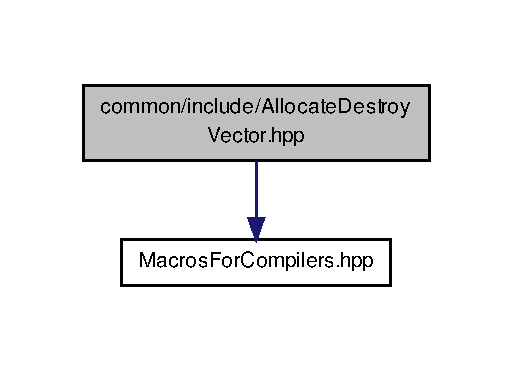
\includegraphics[width=246pt]{AllocateDestroyVector_8hpp__incl}
\end{center}
\end{figure}
This graph shows which files directly or indirectly include this file\-:\nopagebreak
\begin{figure}[H]
\begin{center}
\leavevmode
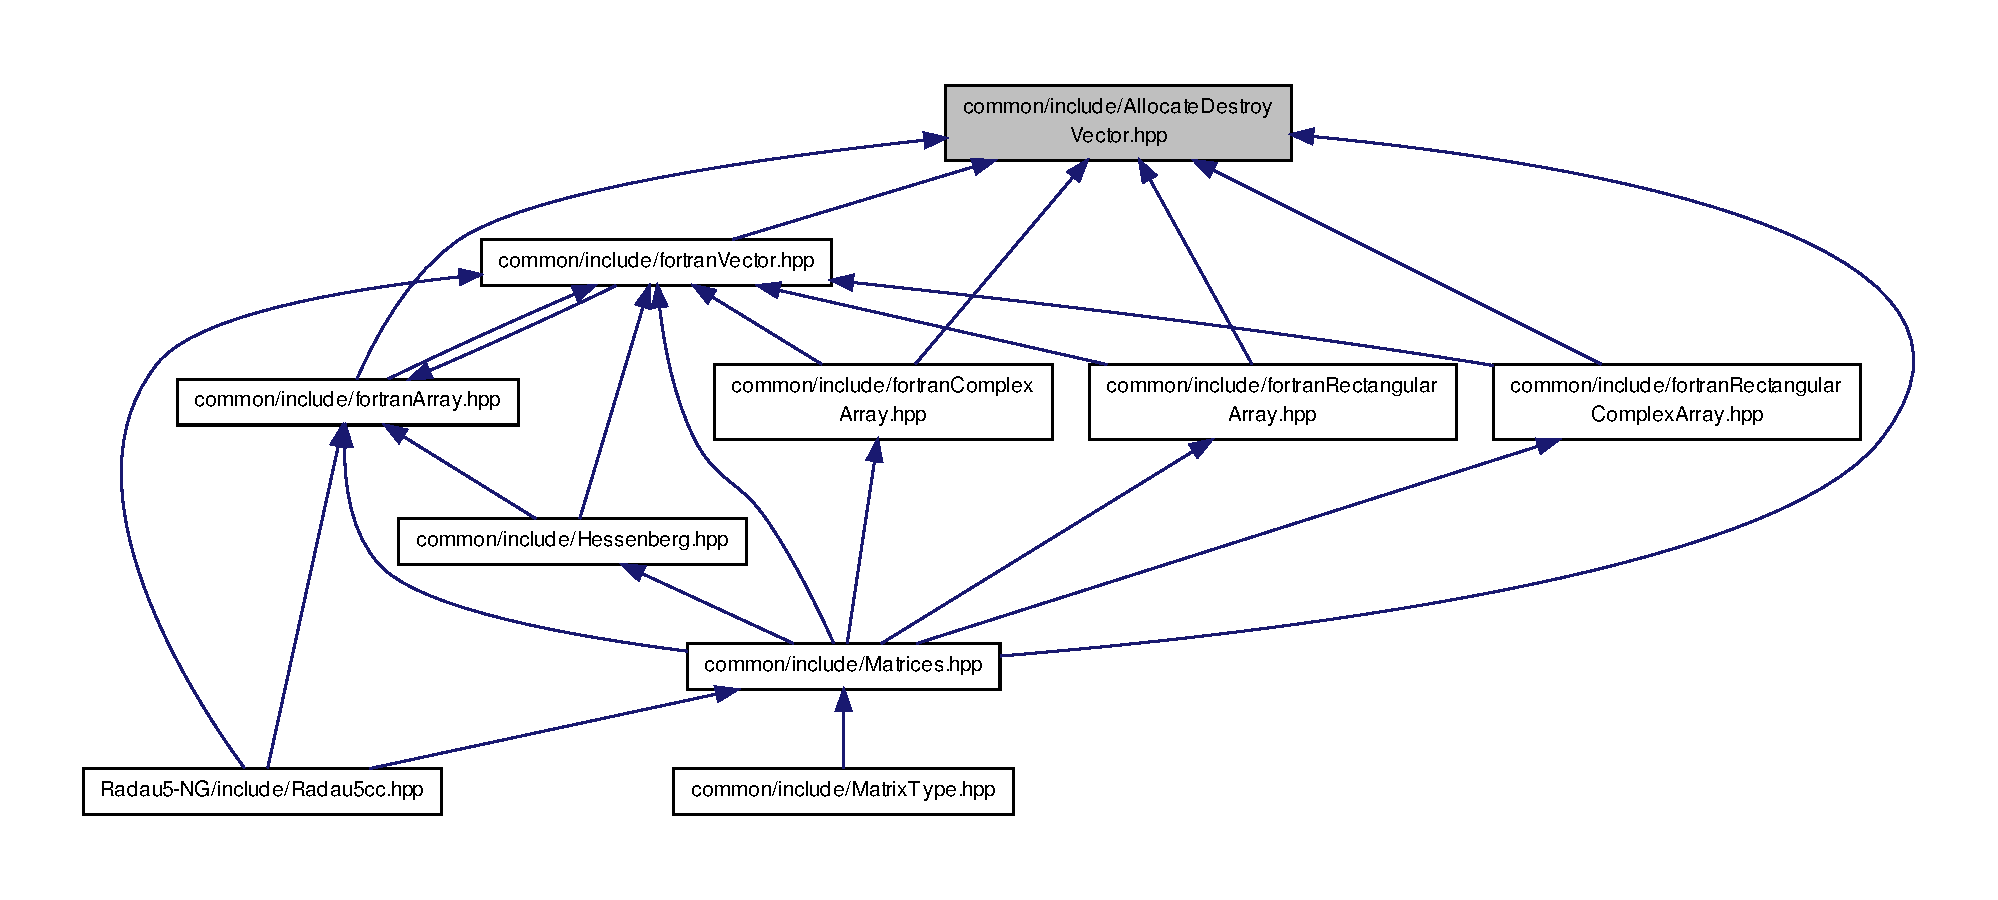
\includegraphics[width=350pt]{AllocateDestroyVector_8hpp__dep__incl}
\end{center}
\end{figure}
\subsection*{Macros}
\begin{DoxyCompactItemize}
\item 
\#define \hyperlink{AllocateDestroyVector_8hpp_a8f41bf13e35e562c37f01267b0b0f061}{A\-S\-S\-U\-M\-E\-\_\-\-A\-L\-I\-G\-N\-E\-D}(lvalueptr)
\end{DoxyCompactItemize}
\subsection*{Functions}
\begin{DoxyCompactItemize}
\item 
double $\ast$ \hyperlink{AllocateDestroyVector_8hpp_a7fd4ca1c3639c1c7ae39b4f31bd17fa3}{alloc\-Double\-Array} (int size)
\begin{DoxyCompactList}\small\item\em Define different methods to allocate arrays. \end{DoxyCompactList}\item 
void \hyperlink{AllocateDestroyVector_8hpp_a31c643df2bd077ef02f98ddcb812abd4}{destroy\-Double\-Array} (double $\ast$x)
\end{DoxyCompactItemize}


\subsection{Macro Definition Documentation}
\hypertarget{AllocateDestroyVector_8hpp_a8f41bf13e35e562c37f01267b0b0f061}{\index{Allocate\-Destroy\-Vector.\-hpp@{Allocate\-Destroy\-Vector.\-hpp}!A\-S\-S\-U\-M\-E\-\_\-\-A\-L\-I\-G\-N\-E\-D@{A\-S\-S\-U\-M\-E\-\_\-\-A\-L\-I\-G\-N\-E\-D}}
\index{A\-S\-S\-U\-M\-E\-\_\-\-A\-L\-I\-G\-N\-E\-D@{A\-S\-S\-U\-M\-E\-\_\-\-A\-L\-I\-G\-N\-E\-D}!AllocateDestroyVector.hpp@{Allocate\-Destroy\-Vector.\-hpp}}
\subsubsection[{A\-S\-S\-U\-M\-E\-\_\-\-A\-L\-I\-G\-N\-E\-D}]{\setlength{\rightskip}{0pt plus 5cm}\#define A\-S\-S\-U\-M\-E\-\_\-\-A\-L\-I\-G\-N\-E\-D(
\begin{DoxyParamCaption}
\item[{}]{lvalueptr}
\end{DoxyParamCaption}
)}}\label{AllocateDestroyVector_8hpp_a8f41bf13e35e562c37f01267b0b0f061}


\subsection{Function Documentation}
\hypertarget{AllocateDestroyVector_8hpp_a7fd4ca1c3639c1c7ae39b4f31bd17fa3}{\index{Allocate\-Destroy\-Vector.\-hpp@{Allocate\-Destroy\-Vector.\-hpp}!alloc\-Double\-Array@{alloc\-Double\-Array}}
\index{alloc\-Double\-Array@{alloc\-Double\-Array}!AllocateDestroyVector.hpp@{Allocate\-Destroy\-Vector.\-hpp}}
\subsubsection[{alloc\-Double\-Array}]{\setlength{\rightskip}{0pt plus 5cm}double$\ast$ alloc\-Double\-Array (
\begin{DoxyParamCaption}
\item[{int}]{size}
\end{DoxyParamCaption}
)}}\label{AllocateDestroyVector_8hpp_a7fd4ca1c3639c1c7ae39b4f31bd17fa3}


Define different methods to allocate arrays. 

\hypertarget{AllocateDestroyVector_8hpp_a31c643df2bd077ef02f98ddcb812abd4}{\index{Allocate\-Destroy\-Vector.\-hpp@{Allocate\-Destroy\-Vector.\-hpp}!destroy\-Double\-Array@{destroy\-Double\-Array}}
\index{destroy\-Double\-Array@{destroy\-Double\-Array}!AllocateDestroyVector.hpp@{Allocate\-Destroy\-Vector.\-hpp}}
\subsubsection[{destroy\-Double\-Array}]{\setlength{\rightskip}{0pt plus 5cm}void destroy\-Double\-Array (
\begin{DoxyParamCaption}
\item[{double $\ast$}]{x}
\end{DoxyParamCaption}
)}}\label{AllocateDestroyVector_8hpp_a31c643df2bd077ef02f98ddcb812abd4}

\hypertarget{compat_8hpp}{\section{common/include/compat.hpp File Reference}
\label{compat_8hpp}\index{common/include/compat.\-hpp@{common/include/compat.\-hpp}}
}
This graph shows which files directly or indirectly include this file\-:\nopagebreak
\begin{figure}[H]
\begin{center}
\leavevmode
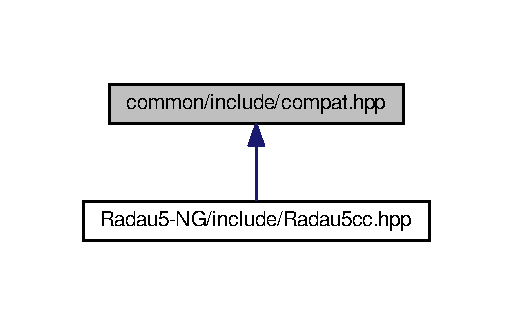
\includegraphics[width=252pt]{compat_8hpp__dep__incl}
\end{center}
\end{figure}
\subsection*{Classes}
\begin{DoxyCompactItemize}
\item 
struct \hyperlink{structcompat}{compat$<$ full, Hessenberg $>$}
\end{DoxyCompactItemize}
\subsection*{Macros}
\begin{DoxyCompactItemize}
\item 
\#define \hyperlink{compat_8hpp_ac41c7fb1ca72aa1768dbc146fe1921c6}{A\-S\-S\-E\-R\-T\-\_\-\-C\-O\-N\-C\-A\-T\-\_\-}(a, b)~a\#\#b
\item 
\#define \hyperlink{compat_8hpp_a9fad378d3538885ffce2b40a29334fbb}{A\-S\-S\-E\-R\-T\-\_\-\-C\-O\-N\-C\-A\-T}(a, b)~\hyperlink{compat_8hpp_ac41c7fb1ca72aa1768dbc146fe1921c6}{A\-S\-S\-E\-R\-T\-\_\-\-C\-O\-N\-C\-A\-T\-\_\-}(a, b)
\item 
\#define \hyperlink{compat_8hpp_a27fc2521d61e2a71685d420b2ffe30c6}{ct\-\_\-assert}(e)~enum \{ \hyperlink{compat_8hpp_a9fad378d3538885ffce2b40a29334fbb}{A\-S\-S\-E\-R\-T\-\_\-\-C\-O\-N\-C\-A\-T}(assert\-\_\-line\-\_\-, \-\_\-\-\_\-\-L\-I\-N\-E\-\_\-\-\_\-) = 1/(!!(e)) \}
\end{DoxyCompactItemize}


\subsection{Macro Definition Documentation}
\hypertarget{compat_8hpp_a9fad378d3538885ffce2b40a29334fbb}{\index{compat.\-hpp@{compat.\-hpp}!A\-S\-S\-E\-R\-T\-\_\-\-C\-O\-N\-C\-A\-T@{A\-S\-S\-E\-R\-T\-\_\-\-C\-O\-N\-C\-A\-T}}
\index{A\-S\-S\-E\-R\-T\-\_\-\-C\-O\-N\-C\-A\-T@{A\-S\-S\-E\-R\-T\-\_\-\-C\-O\-N\-C\-A\-T}!compat.hpp@{compat.\-hpp}}
\subsubsection[{A\-S\-S\-E\-R\-T\-\_\-\-C\-O\-N\-C\-A\-T}]{\setlength{\rightskip}{0pt plus 5cm}\#define A\-S\-S\-E\-R\-T\-\_\-\-C\-O\-N\-C\-A\-T(
\begin{DoxyParamCaption}
\item[{}]{a, }
\item[{}]{b}
\end{DoxyParamCaption}
)~{\bf A\-S\-S\-E\-R\-T\-\_\-\-C\-O\-N\-C\-A\-T\-\_\-}(a, b)}}\label{compat_8hpp_a9fad378d3538885ffce2b40a29334fbb}
\hypertarget{compat_8hpp_ac41c7fb1ca72aa1768dbc146fe1921c6}{\index{compat.\-hpp@{compat.\-hpp}!A\-S\-S\-E\-R\-T\-\_\-\-C\-O\-N\-C\-A\-T\-\_\-@{A\-S\-S\-E\-R\-T\-\_\-\-C\-O\-N\-C\-A\-T\-\_\-}}
\index{A\-S\-S\-E\-R\-T\-\_\-\-C\-O\-N\-C\-A\-T\-\_\-@{A\-S\-S\-E\-R\-T\-\_\-\-C\-O\-N\-C\-A\-T\-\_\-}!compat.hpp@{compat.\-hpp}}
\subsubsection[{A\-S\-S\-E\-R\-T\-\_\-\-C\-O\-N\-C\-A\-T\-\_\-}]{\setlength{\rightskip}{0pt plus 5cm}\#define A\-S\-S\-E\-R\-T\-\_\-\-C\-O\-N\-C\-A\-T\-\_\-(
\begin{DoxyParamCaption}
\item[{}]{a, }
\item[{}]{b}
\end{DoxyParamCaption}
)~a\#\#b}}\label{compat_8hpp_ac41c7fb1ca72aa1768dbc146fe1921c6}
\hypertarget{compat_8hpp_a27fc2521d61e2a71685d420b2ffe30c6}{\index{compat.\-hpp@{compat.\-hpp}!ct\-\_\-assert@{ct\-\_\-assert}}
\index{ct\-\_\-assert@{ct\-\_\-assert}!compat.hpp@{compat.\-hpp}}
\subsubsection[{ct\-\_\-assert}]{\setlength{\rightskip}{0pt plus 5cm}\#define ct\-\_\-assert(
\begin{DoxyParamCaption}
\item[{}]{e}
\end{DoxyParamCaption}
)~enum \{ {\bf A\-S\-S\-E\-R\-T\-\_\-\-C\-O\-N\-C\-A\-T}(assert\-\_\-line\-\_\-, \-\_\-\-\_\-\-L\-I\-N\-E\-\_\-\-\_\-) = 1/(!!(e)) \}}}\label{compat_8hpp_a27fc2521d61e2a71685d420b2ffe30c6}

\hypertarget{fortranArray_8hpp}{}\section{common/include/fortran\+Array.hpp File Reference}
\label{fortranArray_8hpp}\index{common/include/fortran\+Array.\+hpp@{common/include/fortran\+Array.\+hpp}}
{\ttfamily \#include \char`\"{}fortran\+Vector.\+hpp\char`\"{}}\\*
{\ttfamily \#include \char`\"{}Generic\+Exception.\+hpp\char`\"{}}\\*
{\ttfamily \#include $<$string$>$}\\*
{\ttfamily \#include $<$iostream$>$}\\*
{\ttfamily \#include \char`\"{}Allocate\+Destroy\+Vector.\+hpp\char`\"{}}\\*
{\ttfamily \#include \char`\"{}Ivdep.\+hpp\char`\"{}}\\*
Include dependency graph for fortran\+Array.\+hpp\+:
\nopagebreak
\begin{figure}[H]
\begin{center}
\leavevmode
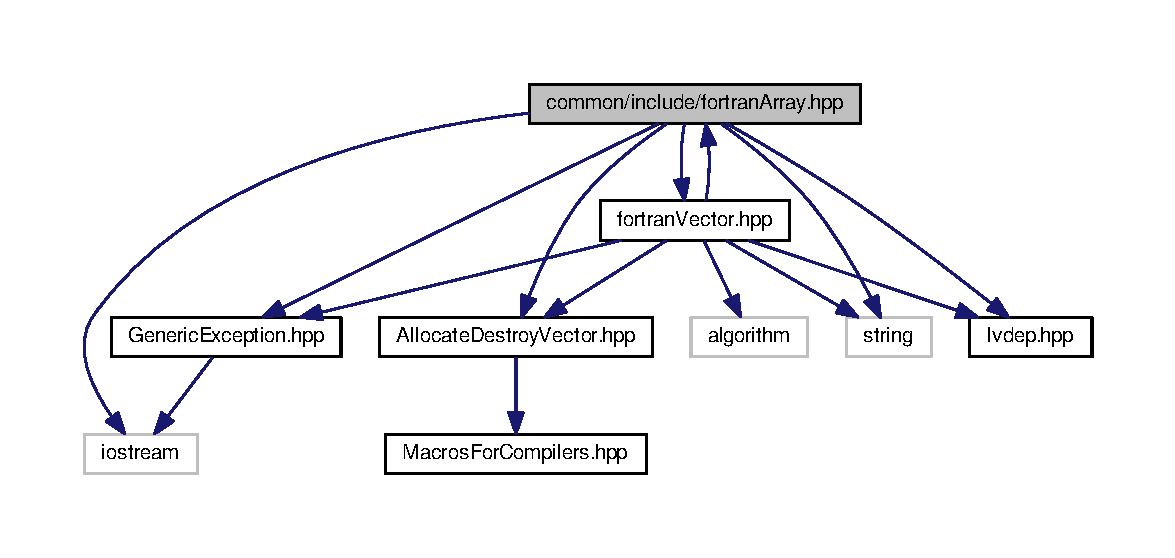
\includegraphics[width=350pt]{fortranArray_8hpp__incl}
\end{center}
\end{figure}
This graph shows which files directly or indirectly include this file\+:
\nopagebreak
\begin{figure}[H]
\begin{center}
\leavevmode
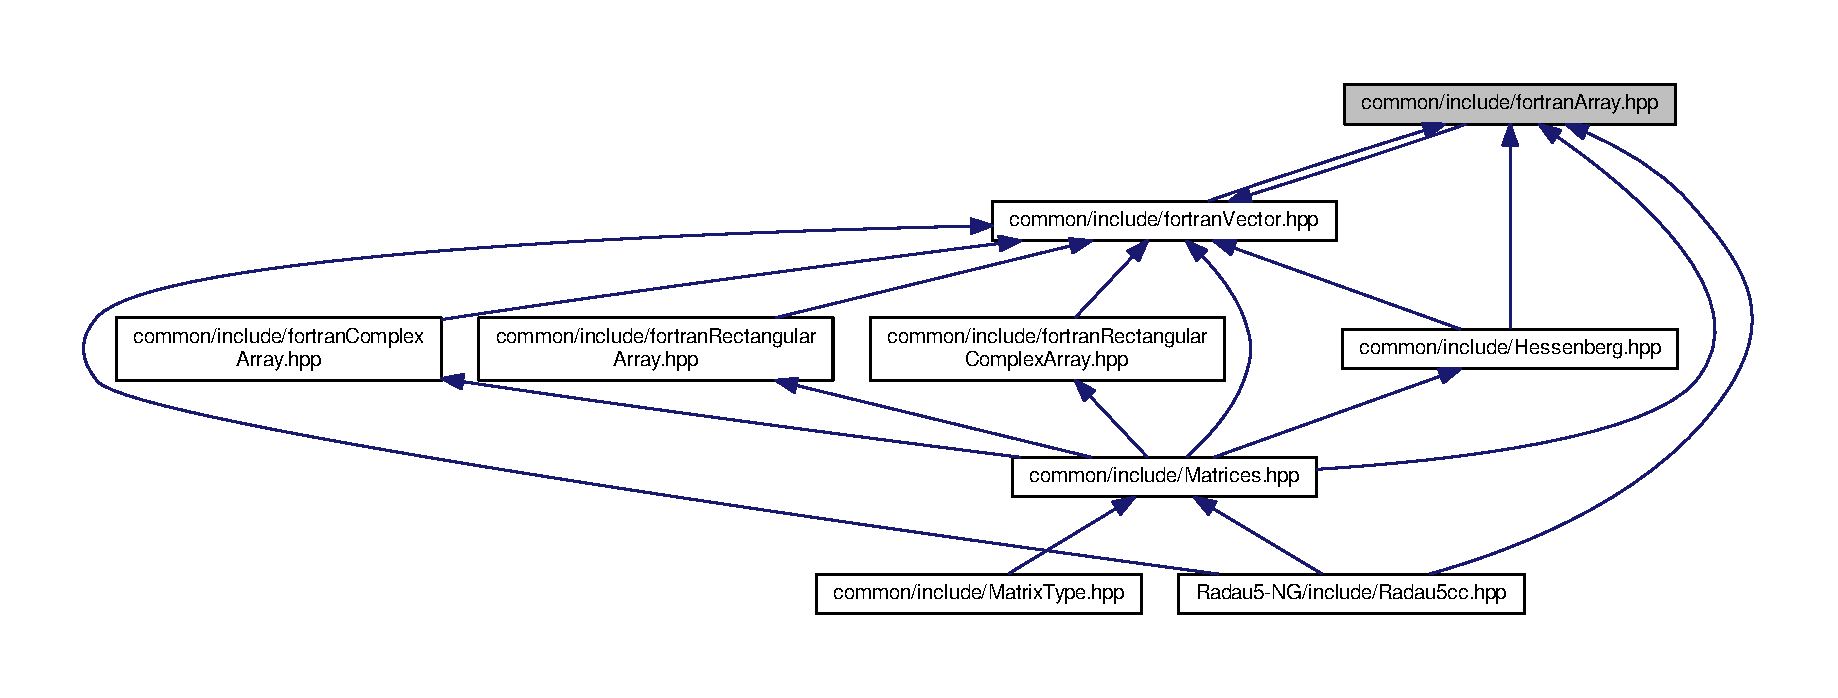
\includegraphics[width=350pt]{fortranArray_8hpp__dep__incl}
\end{center}
\end{figure}
\subsection*{Classes}
\begin{DoxyCompactItemize}
\item 
class \hyperlink{classodes_1_1fortranArray}{odes\+::fortran\+Array$<$ n $>$}
\begin{DoxyCompactList}\small\item\em Array of double. \end{DoxyCompactList}\end{DoxyCompactItemize}
\subsection*{Namespaces}
\begin{DoxyCompactItemize}
\item 
 \hyperlink{namespaceodes}{odes}
\begin{DoxyCompactList}\small\item\em Compute all matrix operations. \end{DoxyCompactList}\end{DoxyCompactItemize}

\hypertarget{fortranComplexArray_8hpp}{\section{common/include/fortran\-Complex\-Array.hpp File Reference}
\label{fortranComplexArray_8hpp}\index{common/include/fortran\-Complex\-Array.\-hpp@{common/include/fortran\-Complex\-Array.\-hpp}}
}
{\ttfamily \#include \char`\"{}fortran\-Vector.\-hpp\char`\"{}}\\*
{\ttfamily \#include \char`\"{}Generic\-Exception.\-hpp\char`\"{}}\\*
{\ttfamily \#include $<$string$>$}\\*
{\ttfamily \#include $<$iostream$>$}\\*
{\ttfamily \#include \char`\"{}Allocate\-Destroy\-Vector.\-hpp\char`\"{}}\\*
Include dependency graph for fortran\-Complex\-Array.\-hpp\-:\nopagebreak
\begin{figure}[H]
\begin{center}
\leavevmode
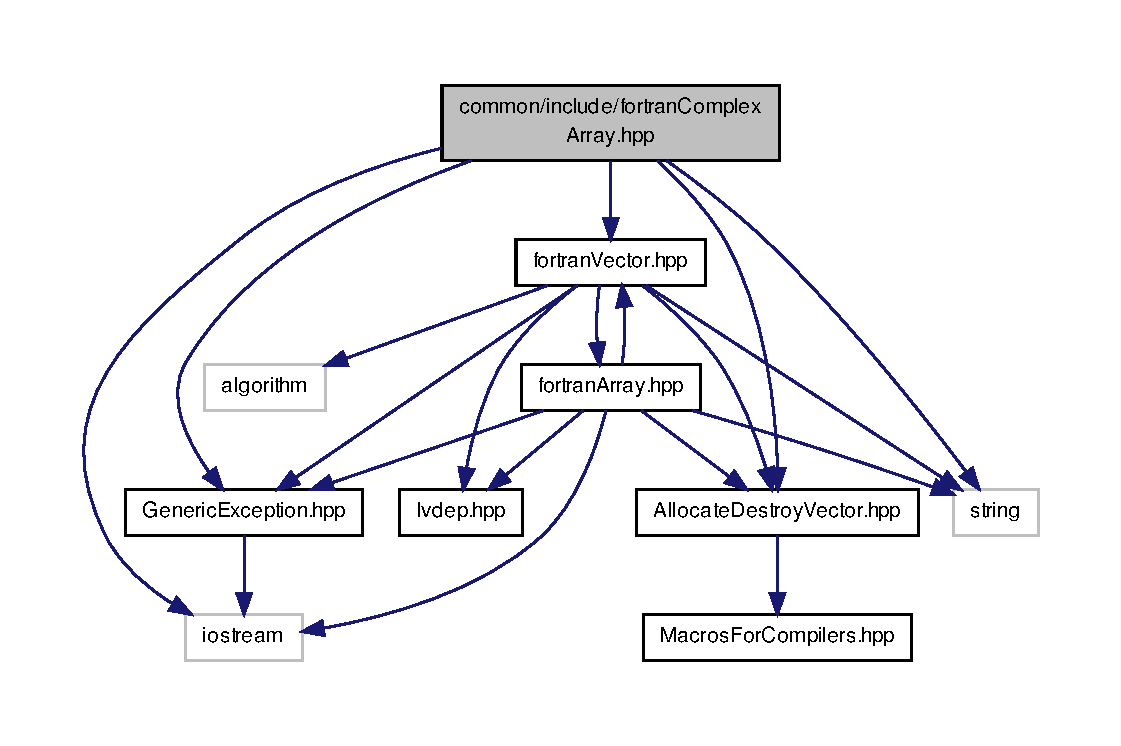
\includegraphics[width=350pt]{fortranComplexArray_8hpp__incl}
\end{center}
\end{figure}
This graph shows which files directly or indirectly include this file\-:\nopagebreak
\begin{figure}[H]
\begin{center}
\leavevmode
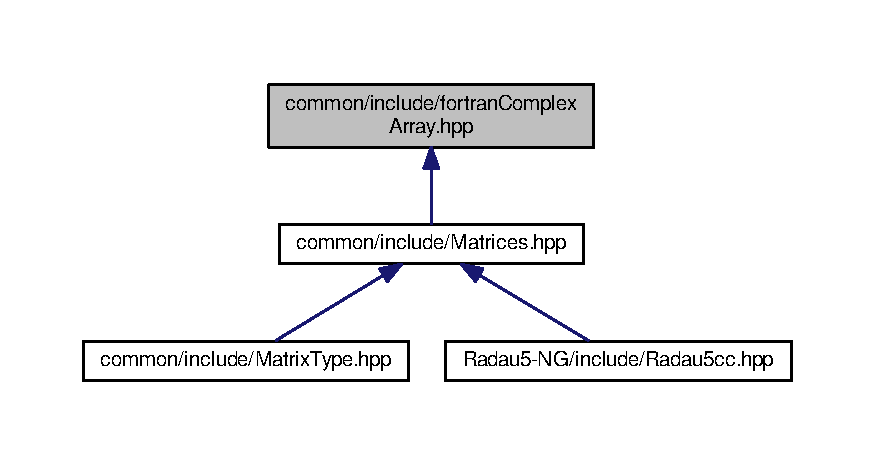
\includegraphics[width=350pt]{fortranComplexArray_8hpp__dep__incl}
\end{center}
\end{figure}
\subsection*{Classes}
\begin{DoxyCompactItemize}
\item 
class \hyperlink{classodes_1_1fortranComplexArray}{odes\-::fortran\-Complex\-Array$<$ n $>$}
\begin{DoxyCompactList}\small\item\em Array of complex.. \end{DoxyCompactList}\end{DoxyCompactItemize}
\subsection*{Namespaces}
\begin{DoxyCompactItemize}
\item 
\hyperlink{namespaceodes}{odes}
\begin{DoxyCompactList}\small\item\em Compute all matrix operations. \end{DoxyCompactList}\end{DoxyCompactItemize}

\hypertarget{fortranRectangularArray_8hpp}{}\section{common/include/fortran\+Rectangular\+Array.hpp File Reference}
\label{fortranRectangularArray_8hpp}\index{common/include/fortran\+Rectangular\+Array.\+hpp@{common/include/fortran\+Rectangular\+Array.\+hpp}}
{\ttfamily \#include \char`\"{}fortran\+Vector.\+hpp\char`\"{}}\\*
{\ttfamily \#include \char`\"{}Generic\+Exception.\+hpp\char`\"{}}\\*
{\ttfamily \#include \char`\"{}Allocate\+Destroy\+Vector.\+hpp\char`\"{}}\\*
{\ttfamily \#include $<$string$>$}\\*
{\ttfamily \#include $<$iostream$>$}\\*
{\ttfamily \#include \char`\"{}Ivdep.\+hpp\char`\"{}}\\*
Include dependency graph for fortran\+Rectangular\+Array.\+hpp\+:
\nopagebreak
\begin{figure}[H]
\begin{center}
\leavevmode
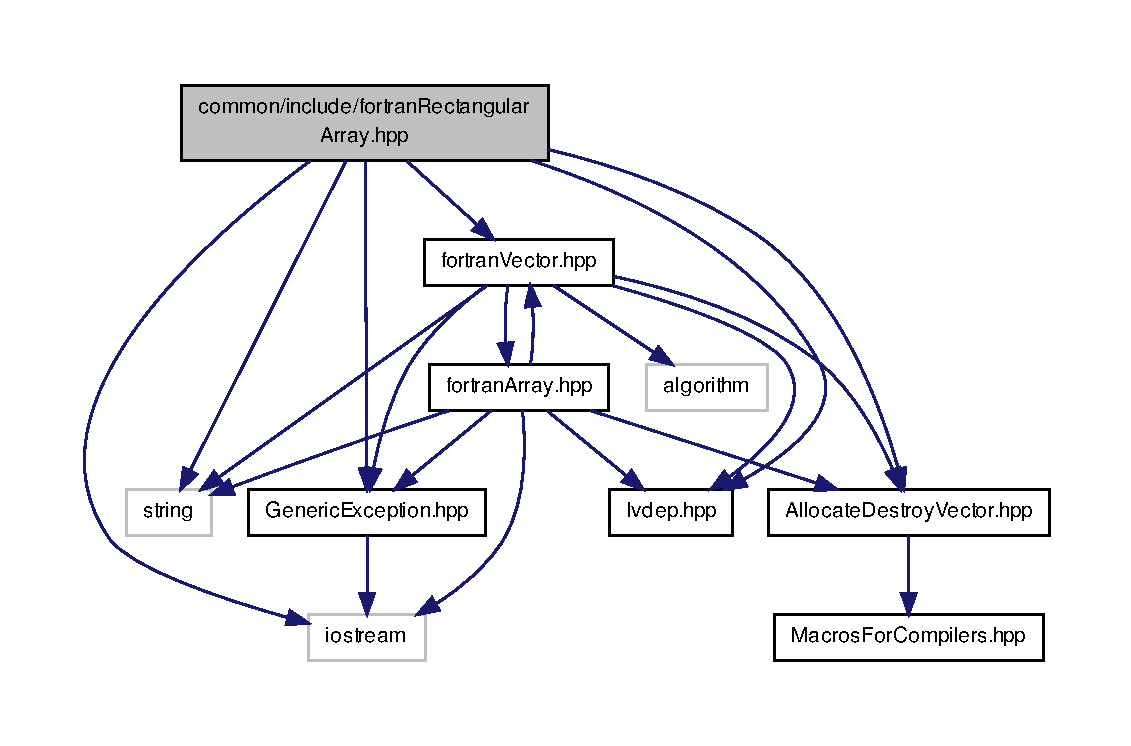
\includegraphics[width=350pt]{fortranRectangularArray_8hpp__incl}
\end{center}
\end{figure}
This graph shows which files directly or indirectly include this file\+:
\nopagebreak
\begin{figure}[H]
\begin{center}
\leavevmode
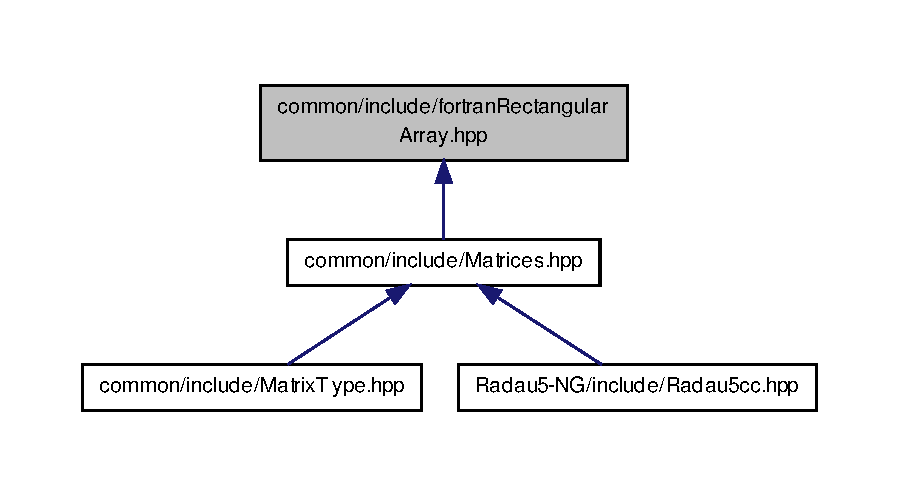
\includegraphics[width=350pt]{fortranRectangularArray_8hpp__dep__incl}
\end{center}
\end{figure}
\subsection*{Classes}
\begin{DoxyCompactItemize}
\item 
class \hyperlink{classodes_1_1fortranRectangularArray}{odes\+::fortran\+Rectangular\+Array$<$ n, kl, ku $>$}
\begin{DoxyCompactList}\small\item\em Banded Array of double. \end{DoxyCompactList}\end{DoxyCompactItemize}
\subsection*{Namespaces}
\begin{DoxyCompactItemize}
\item 
 \hyperlink{namespaceodes}{odes}
\begin{DoxyCompactList}\small\item\em Compute all matrix operations. \end{DoxyCompactList}\end{DoxyCompactItemize}
\subsection*{Macros}
\begin{DoxyCompactItemize}
\item 
\#define \hyperlink{fortranRectangularArray_8hpp_aacc3ee1a7f283f8ef65cea31f4436a95}{M\+A\+X}(x,  y)~((x)$>$(y)?(x)\+:(y))
\item 
\#define \hyperlink{fortranRectangularArray_8hpp_a74e75242132eaabbc1c512488a135926}{M\+I\+N}(x,  y)~((x)$<$(y)?(x)\+:(y))
\end{DoxyCompactItemize}


\subsection{Macro Definition Documentation}
\hypertarget{fortranRectangularArray_8hpp_aacc3ee1a7f283f8ef65cea31f4436a95}{}\index{fortran\+Rectangular\+Array.\+hpp@{fortran\+Rectangular\+Array.\+hpp}!M\+A\+X@{M\+A\+X}}
\index{M\+A\+X@{M\+A\+X}!fortran\+Rectangular\+Array.\+hpp@{fortran\+Rectangular\+Array.\+hpp}}
\subsubsection[{M\+A\+X}]{\setlength{\rightskip}{0pt plus 5cm}\#define M\+A\+X(
\begin{DoxyParamCaption}
\item[{}]{x, }
\item[{}]{y}
\end{DoxyParamCaption}
)~((x)$>$(y)?(x)\+:(y))}\label{fortranRectangularArray_8hpp_aacc3ee1a7f283f8ef65cea31f4436a95}
\hypertarget{fortranRectangularArray_8hpp_a74e75242132eaabbc1c512488a135926}{}\index{fortran\+Rectangular\+Array.\+hpp@{fortran\+Rectangular\+Array.\+hpp}!M\+I\+N@{M\+I\+N}}
\index{M\+I\+N@{M\+I\+N}!fortran\+Rectangular\+Array.\+hpp@{fortran\+Rectangular\+Array.\+hpp}}
\subsubsection[{M\+I\+N}]{\setlength{\rightskip}{0pt plus 5cm}\#define M\+I\+N(
\begin{DoxyParamCaption}
\item[{}]{x, }
\item[{}]{y}
\end{DoxyParamCaption}
)~((x)$<$(y)?(x)\+:(y))}\label{fortranRectangularArray_8hpp_a74e75242132eaabbc1c512488a135926}

\hypertarget{fortranRectangularComplexArray_8hpp}{\section{common/include/fortran\-Rectangular\-Complex\-Array.hpp File Reference}
\label{fortranRectangularComplexArray_8hpp}\index{common/include/fortran\-Rectangular\-Complex\-Array.\-hpp@{common/include/fortran\-Rectangular\-Complex\-Array.\-hpp}}
}
{\ttfamily \#include \char`\"{}fortran\-Vector.\-hpp\char`\"{}}\\*
{\ttfamily \#include \char`\"{}Generic\-Exception.\-hpp\char`\"{}}\\*
{\ttfamily \#include \char`\"{}Allocate\-Destroy\-Vector.\-hpp\char`\"{}}\\*
{\ttfamily \#include $<$string$>$}\\*
{\ttfamily \#include $<$iostream$>$}\\*
Include dependency graph for fortran\-Rectangular\-Complex\-Array.\-hpp\-:\nopagebreak
\begin{figure}[H]
\begin{center}
\leavevmode
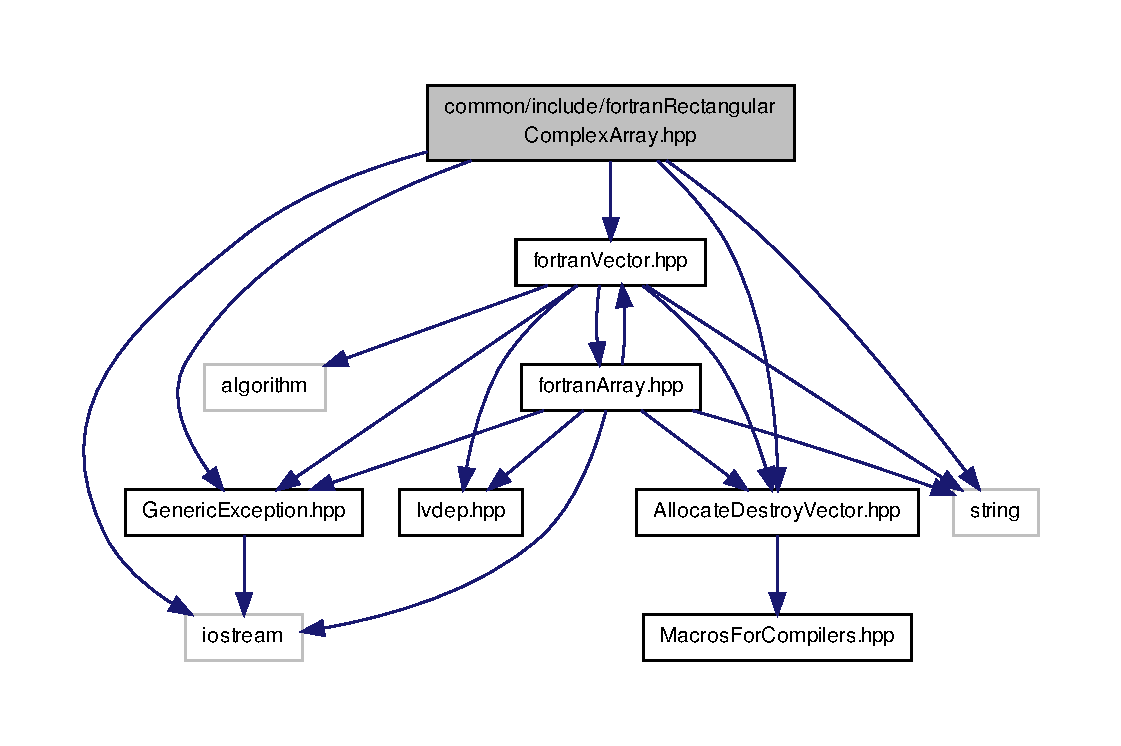
\includegraphics[width=350pt]{fortranRectangularComplexArray_8hpp__incl}
\end{center}
\end{figure}
This graph shows which files directly or indirectly include this file\-:\nopagebreak
\begin{figure}[H]
\begin{center}
\leavevmode
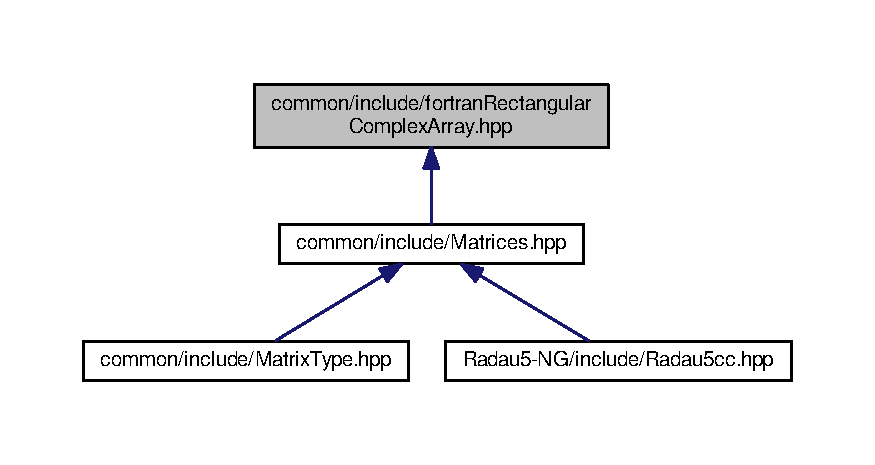
\includegraphics[width=350pt]{fortranRectangularComplexArray_8hpp__dep__incl}
\end{center}
\end{figure}
\subsection*{Classes}
\begin{DoxyCompactItemize}
\item 
class \hyperlink{classodes_1_1fortranRectangularComplexArray}{odes\-::fortran\-Rectangular\-Complex\-Array$<$ n, kl, ku $>$}
\begin{DoxyCompactList}\small\item\em Banded Array of complex.. \end{DoxyCompactList}\end{DoxyCompactItemize}
\subsection*{Namespaces}
\begin{DoxyCompactItemize}
\item 
\hyperlink{namespaceodes}{odes}
\begin{DoxyCompactList}\small\item\em Compute all matrix operations. \end{DoxyCompactList}\end{DoxyCompactItemize}
\subsection*{Macros}
\begin{DoxyCompactItemize}
\item 
\#define \hyperlink{fortranRectangularComplexArray_8hpp_aacc3ee1a7f283f8ef65cea31f4436a95}{M\-A\-X}(x, y)~((x)$>$(y)?(x)\-:(y))
\item 
\#define \hyperlink{fortranRectangularComplexArray_8hpp_a74e75242132eaabbc1c512488a135926}{M\-I\-N}(x, y)~((x)$<$(y)?(x)\-:(y))
\end{DoxyCompactItemize}


\subsection{Macro Definition Documentation}
\hypertarget{fortranRectangularComplexArray_8hpp_aacc3ee1a7f283f8ef65cea31f4436a95}{\index{fortran\-Rectangular\-Complex\-Array.\-hpp@{fortran\-Rectangular\-Complex\-Array.\-hpp}!M\-A\-X@{M\-A\-X}}
\index{M\-A\-X@{M\-A\-X}!fortranRectangularComplexArray.hpp@{fortran\-Rectangular\-Complex\-Array.\-hpp}}
\subsubsection[{M\-A\-X}]{\setlength{\rightskip}{0pt plus 5cm}\#define M\-A\-X(
\begin{DoxyParamCaption}
\item[{}]{x, }
\item[{}]{y}
\end{DoxyParamCaption}
)~((x)$>$(y)?(x)\-:(y))}}\label{fortranRectangularComplexArray_8hpp_aacc3ee1a7f283f8ef65cea31f4436a95}
\hypertarget{fortranRectangularComplexArray_8hpp_a74e75242132eaabbc1c512488a135926}{\index{fortran\-Rectangular\-Complex\-Array.\-hpp@{fortran\-Rectangular\-Complex\-Array.\-hpp}!M\-I\-N@{M\-I\-N}}
\index{M\-I\-N@{M\-I\-N}!fortranRectangularComplexArray.hpp@{fortran\-Rectangular\-Complex\-Array.\-hpp}}
\subsubsection[{M\-I\-N}]{\setlength{\rightskip}{0pt plus 5cm}\#define M\-I\-N(
\begin{DoxyParamCaption}
\item[{}]{x, }
\item[{}]{y}
\end{DoxyParamCaption}
)~((x)$<$(y)?(x)\-:(y))}}\label{fortranRectangularComplexArray_8hpp_a74e75242132eaabbc1c512488a135926}

\hypertarget{fortranVector_8hpp}{\section{common/include/fortran\-Vector.hpp File Reference}
\label{fortranVector_8hpp}\index{common/include/fortran\-Vector.\-hpp@{common/include/fortran\-Vector.\-hpp}}
}
{\ttfamily \#include \char`\"{}Generic\-Exception.\-hpp\char`\"{}}\\*
{\ttfamily \#include \char`\"{}fortran\-Array.\-hpp\char`\"{}}\\*
{\ttfamily \#include \char`\"{}Allocate\-Destroy\-Vector.\-hpp\char`\"{}}\\*
{\ttfamily \#include $<$algorithm$>$}\\*
{\ttfamily \#include $<$string$>$}\\*
{\ttfamily \#include \char`\"{}Ivdep.\-hpp\char`\"{}}\\*
Include dependency graph for fortran\-Vector.\-hpp\-:\nopagebreak
\begin{figure}[H]
\begin{center}
\leavevmode
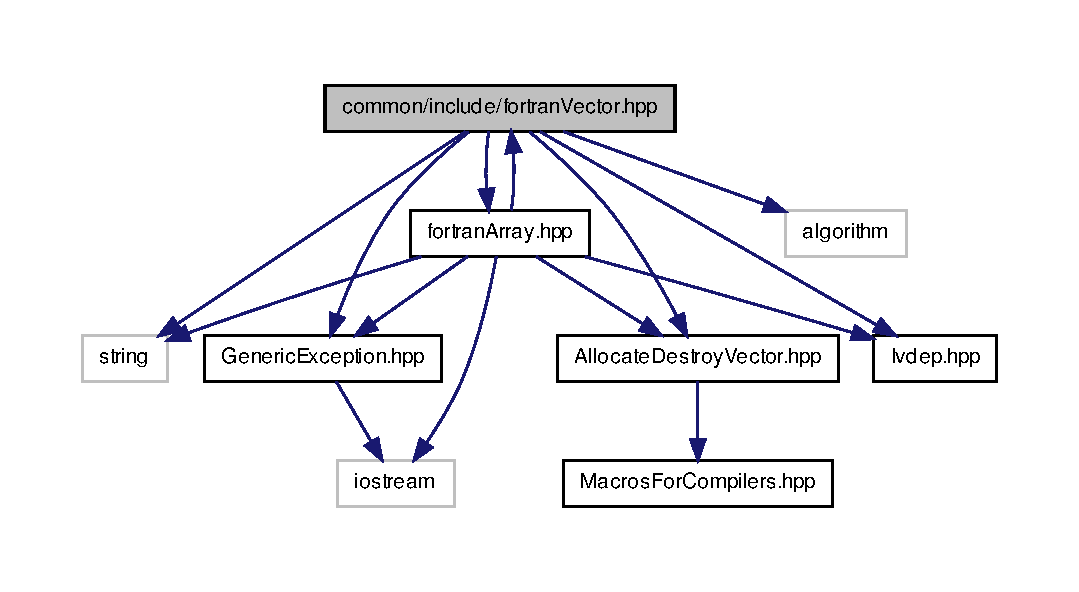
\includegraphics[width=350pt]{fortranVector_8hpp__incl}
\end{center}
\end{figure}
This graph shows which files directly or indirectly include this file\-:\nopagebreak
\begin{figure}[H]
\begin{center}
\leavevmode
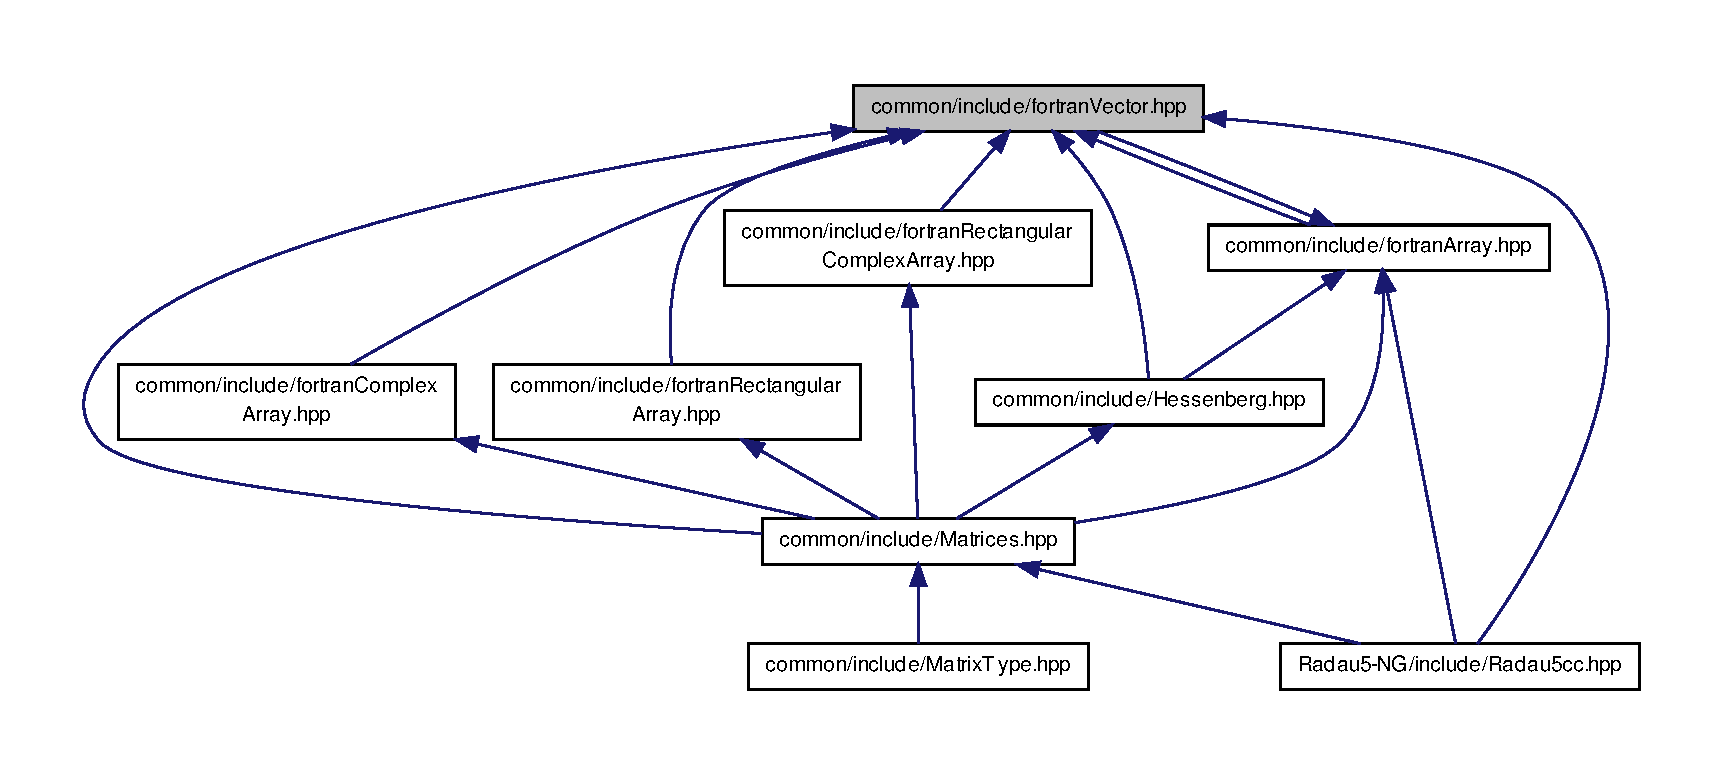
\includegraphics[width=350pt]{fortranVector_8hpp__dep__incl}
\end{center}
\end{figure}
\subsection*{Classes}
\begin{DoxyCompactItemize}
\item 
class \hyperlink{classodes_1_1fortranVector}{odes\-::fortran\-Vector}
\begin{DoxyCompactList}\small\item\em Vector class (of doubles). \end{DoxyCompactList}\item 
class \hyperlink{classodes_1_1fortranVectorF}{odes\-::fortran\-Vector\-F$<$ n $>$}
\begin{DoxyCompactList}\small\item\em Vector class (of doubles). \end{DoxyCompactList}\end{DoxyCompactItemize}
\subsection*{Namespaces}
\begin{DoxyCompactItemize}
\item 
\hyperlink{namespaceodes}{odes}
\begin{DoxyCompactList}\small\item\em Compute all matrix operations. \end{DoxyCompactList}\end{DoxyCompactItemize}

\hypertarget{GenericException_8hpp}{\section{common/include/\-Generic\-Exception.hpp File Reference}
\label{GenericException_8hpp}\index{common/include/\-Generic\-Exception.\-hpp@{common/include/\-Generic\-Exception.\-hpp}}
}
{\ttfamily \#include $<$iostream$>$}\\*
Include dependency graph for Generic\-Exception.\-hpp\-:\nopagebreak
\begin{figure}[H]
\begin{center}
\leavevmode
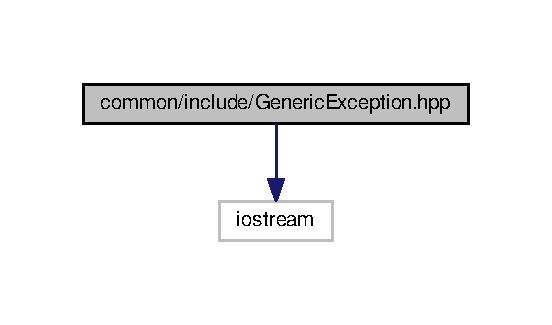
\includegraphics[width=270pt]{GenericException_8hpp__incl}
\end{center}
\end{figure}
This graph shows which files directly or indirectly include this file\-:\nopagebreak
\begin{figure}[H]
\begin{center}
\leavevmode
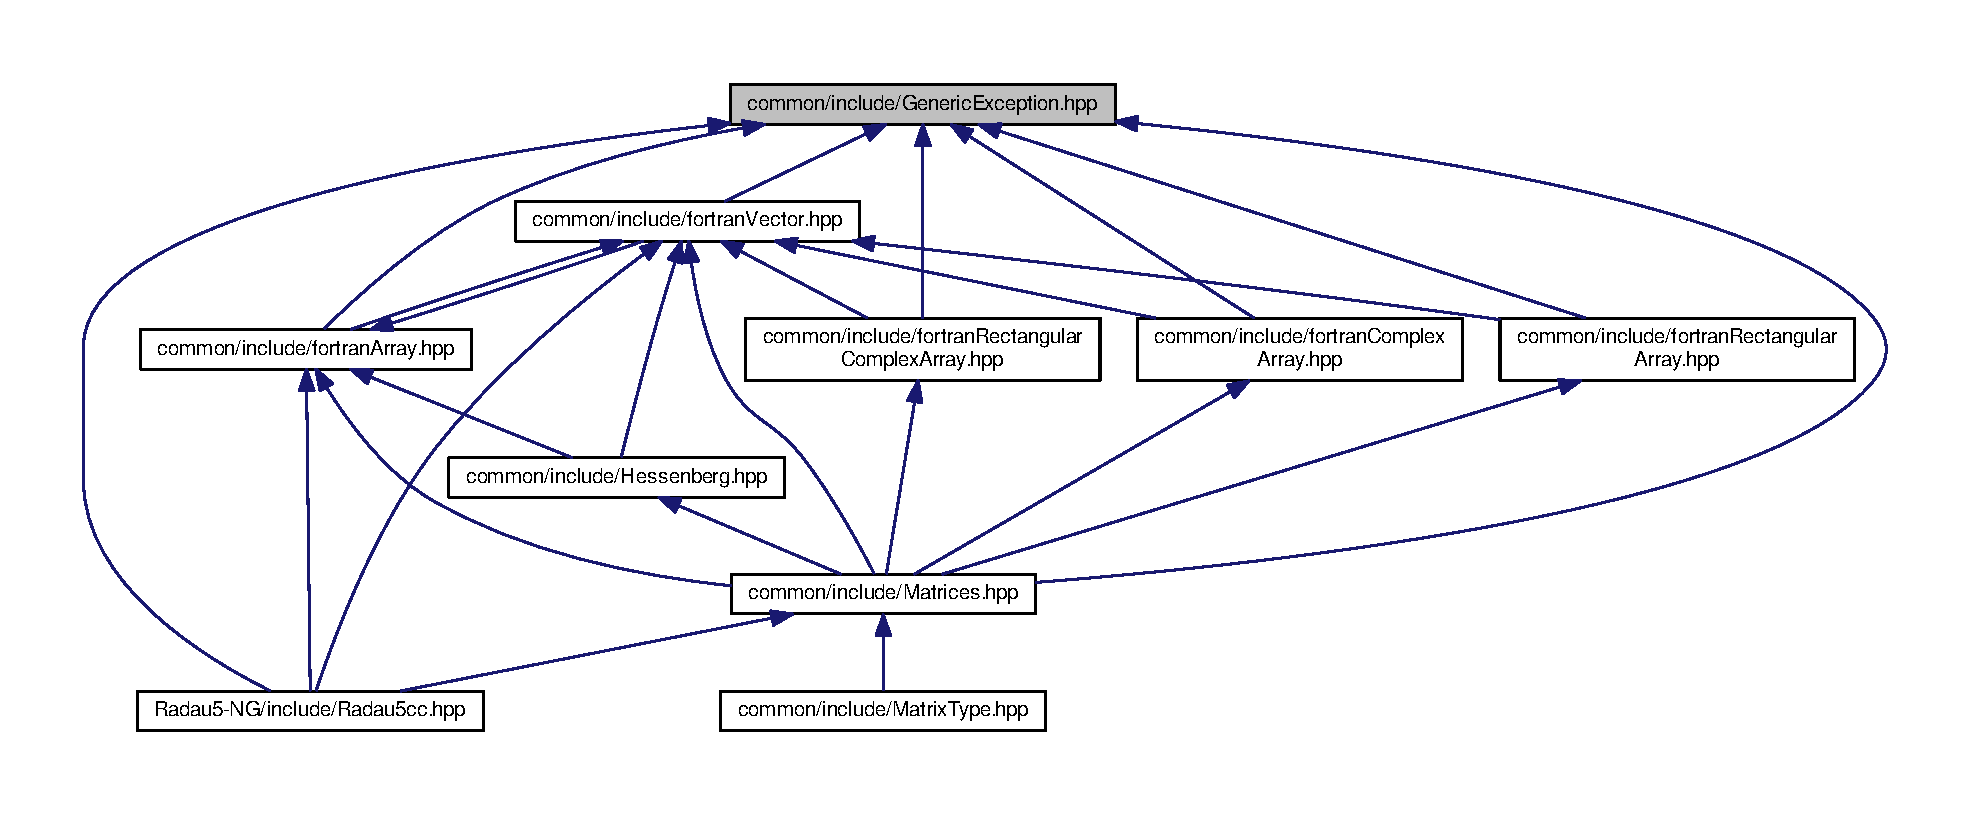
\includegraphics[width=350pt]{GenericException_8hpp__dep__incl}
\end{center}
\end{figure}
\subsection*{Classes}
\begin{DoxyCompactItemize}
\item 
class \hyperlink{classGenericException}{Generic\-Exception}
\end{DoxyCompactItemize}

\hypertarget{Hessenberg_8hpp}{}\section{common/include/\+Hessenberg.hpp File Reference}
\label{Hessenberg_8hpp}\index{common/include/\+Hessenberg.\+hpp@{common/include/\+Hessenberg.\+hpp}}
{\ttfamily \#include \char`\"{}fortran\+Array.\+hpp\char`\"{}}\\*
{\ttfamily \#include \char`\"{}fortran\+Vector.\+hpp\char`\"{}}\\*
Include dependency graph for Hessenberg.\+hpp\+:
\nopagebreak
\begin{figure}[H]
\begin{center}
\leavevmode
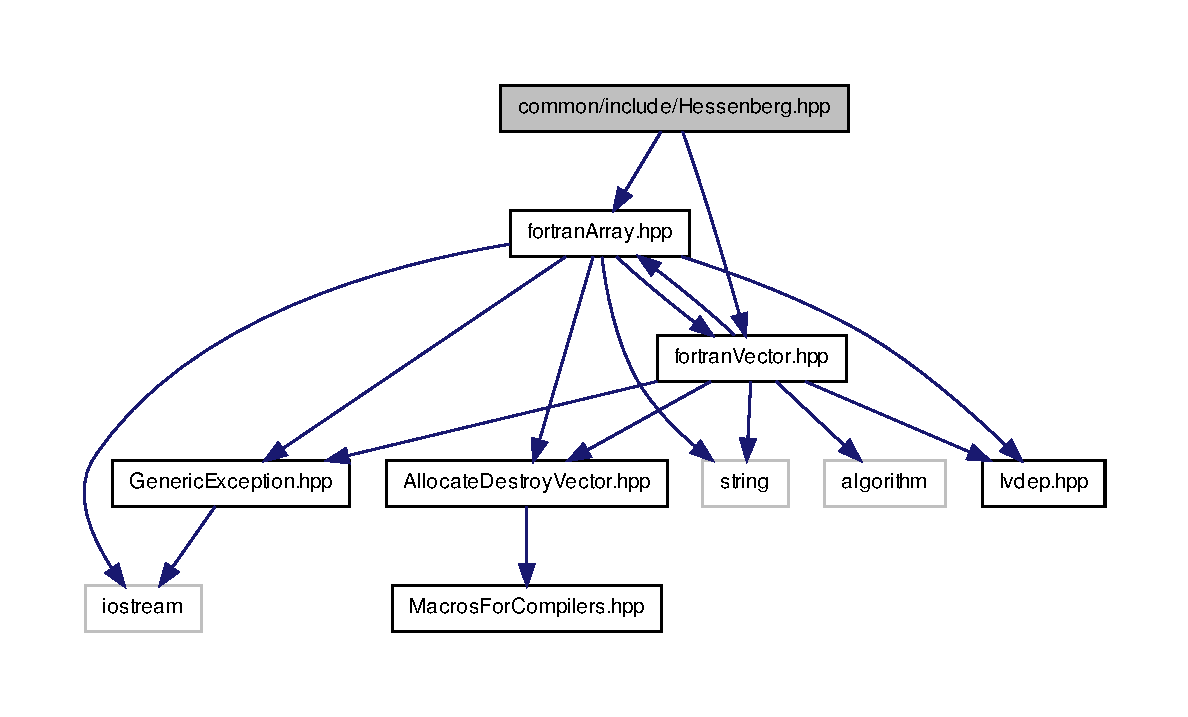
\includegraphics[width=350pt]{Hessenberg_8hpp__incl}
\end{center}
\end{figure}
This graph shows which files directly or indirectly include this file\+:
\nopagebreak
\begin{figure}[H]
\begin{center}
\leavevmode
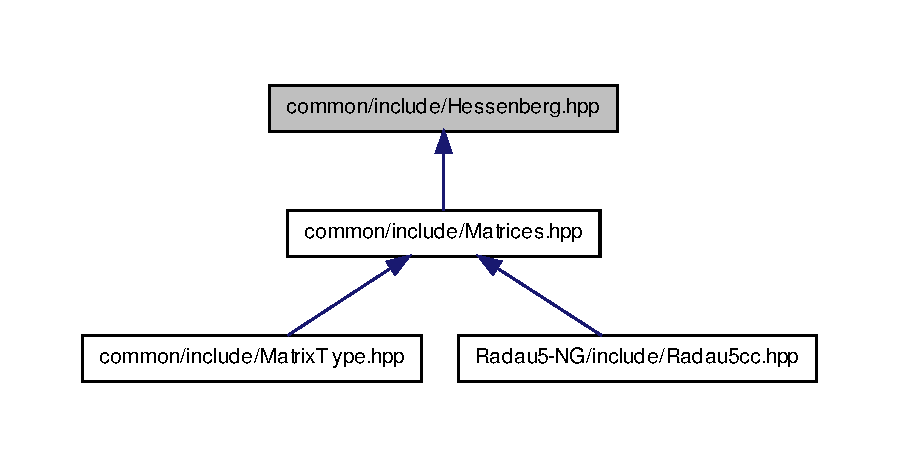
\includegraphics[width=350pt]{Hessenberg_8hpp__dep__incl}
\end{center}
\end{figure}
\subsection*{Macros}
\begin{DoxyCompactItemize}
\item 
\#define \hyperlink{Hessenberg_8hpp_a74e75242132eaabbc1c512488a135926}{M\+I\+N}(x,  y)~((x)$<$(y)?(x)\+:(y))
\item 
\#define \hyperlink{Hessenberg_8hpp_ae2f08dc603ae93c402abd918ba4e23e1}{A\+B\+S}(a)~(((a) $>$= (0.\+0)) ? (a) \+: (-\/a))
\end{DoxyCompactItemize}
\subsection*{Functions}
\begin{DoxyCompactItemize}
\item 
{\footnotesize template$<$int n$>$ }\\int \hyperlink{Hessenberg_8hpp_a8b6132799c779c907ed992fb0dd68a45}{dech} (\hyperlink{classodes_1_1fortranArray}{fortran\+Array}$<$ n $>$ \&A, int ip\mbox{[}$\,$\mbox{]})
\begin{DoxyCompactList}\small\item\em Triangularization by Gaussian elimination of a Hessenberk Matrix. \end{DoxyCompactList}\item 
{\footnotesize template$<$int n$>$ }\\void \hyperlink{Hessenberg_8hpp_aa30d03b19dd5fefaf55643a20d6a865a}{solh} (const \hyperlink{classodes_1_1fortranArray}{fortran\+Array}$<$ n $>$ \&A, const int ip\mbox{[}$\,$\mbox{]}, \hyperlink{classodes_1_1fortranVector}{fortran\+Vector} \&B)
\item 
{\footnotesize template$<$int n$>$ }\\int \hyperlink{Hessenberg_8hpp_a266d75348673cf099ded7434558a73e5}{dechc} (\hyperlink{classodes_1_1fortranArray}{fortran\+Array}$<$ n $>$ \&Ar, \hyperlink{classodes_1_1fortranArray}{fortran\+Array}$<$ n $>$ \&Ai, int ip\mbox{[}$\,$\mbox{]})
\begin{DoxyCompactList}\small\item\em Triangularization by Gaussian elimination of a complex. \end{DoxyCompactList}\item 
{\footnotesize template$<$int n$>$ }\\void \hyperlink{Hessenberg_8hpp_a1f58477a1574c6211ac203cd2ecd8168}{solhc} (const \hyperlink{classodes_1_1fortranArray}{fortran\+Array}$<$ n $>$ \&Ar, const \hyperlink{classodes_1_1fortranArray}{fortran\+Array}$<$ n $>$ \&Ai, const int ip\mbox{[}$\,$\mbox{]}, \hyperlink{classodes_1_1fortranVector}{fortran\+Vector} \&Br, \hyperlink{classodes_1_1fortranVector}{fortran\+Vector} \&Bi)
\item 
{\footnotesize template$<$int n$>$ }\\void \hyperlink{Hessenberg_8hpp_ab7cdcf7b806d715c7190aed95554c14d}{householder} (const \hyperlink{classodes_1_1fortranArray}{fortran\+Array}$<$ n $>$ \&A, const double tau\mbox{[}$\,$\mbox{]}, const \hyperlink{classodes_1_1fortranVector}{fortran\+Vector} \&X, \hyperlink{classodes_1_1fortranVector}{fortran\+Vector} \&Y, bool direct)
\end{DoxyCompactItemize}


\subsection{Macro Definition Documentation}
\hypertarget{Hessenberg_8hpp_ae2f08dc603ae93c402abd918ba4e23e1}{}\index{Hessenberg.\+hpp@{Hessenberg.\+hpp}!A\+B\+S@{A\+B\+S}}
\index{A\+B\+S@{A\+B\+S}!Hessenberg.\+hpp@{Hessenberg.\+hpp}}
\subsubsection[{A\+B\+S}]{\setlength{\rightskip}{0pt plus 5cm}\#define A\+B\+S(
\begin{DoxyParamCaption}
\item[{}]{a}
\end{DoxyParamCaption}
)~(((a) $>$= (0.\+0)) ? (a) \+: (-\/a))}\label{Hessenberg_8hpp_ae2f08dc603ae93c402abd918ba4e23e1}
\hypertarget{Hessenberg_8hpp_a74e75242132eaabbc1c512488a135926}{}\index{Hessenberg.\+hpp@{Hessenberg.\+hpp}!M\+I\+N@{M\+I\+N}}
\index{M\+I\+N@{M\+I\+N}!Hessenberg.\+hpp@{Hessenberg.\+hpp}}
\subsubsection[{M\+I\+N}]{\setlength{\rightskip}{0pt plus 5cm}\#define M\+I\+N(
\begin{DoxyParamCaption}
\item[{}]{x, }
\item[{}]{y}
\end{DoxyParamCaption}
)~((x)$<$(y)?(x)\+:(y))}\label{Hessenberg_8hpp_a74e75242132eaabbc1c512488a135926}


\subsection{Function Documentation}
\hypertarget{Hessenberg_8hpp_a8b6132799c779c907ed992fb0dd68a45}{}\index{Hessenberg.\+hpp@{Hessenberg.\+hpp}!dech@{dech}}
\index{dech@{dech}!Hessenberg.\+hpp@{Hessenberg.\+hpp}}
\subsubsection[{dech}]{\setlength{\rightskip}{0pt plus 5cm}template$<$int n$>$ int dech (
\begin{DoxyParamCaption}
\item[{{\bf fortran\+Array}$<$ n $>$ \&}]{A, }
\item[{int}]{ip\mbox{[}$\,$\mbox{]}}
\end{DoxyParamCaption}
)}\label{Hessenberg_8hpp_a8b6132799c779c907ed992fb0dd68a45}


Triangularization by Gaussian elimination of a Hessenberk Matrix. 

All what is necessary to compute with Hessenberg matrices (but not the reduction of a full matrix to Hessenberg form (see \hyperlink{Matrices_8hpp}{Matrices.\+hpp}). Triangularization by Gaussian elimination of a Hessenberk Matrix with lower Bandwidth ==1. 
\begin{DoxyParams}{Parameters}
{\em A} & the matrix (I\+N/\+O\+U\+T). \\
\hline
{\em ip} & index of pivots. \\
\hline
\end{DoxyParams}
\begin{DoxyNote}{Note}
return 0 ii everything went well, otherwise the rank wher the matrix A was found singular. 

this is a C++ transcription of D\+E\+C\+H (in H.\&W. fortran code decsol). 
\end{DoxyNote}
\hypertarget{Hessenberg_8hpp_a266d75348673cf099ded7434558a73e5}{}\index{Hessenberg.\+hpp@{Hessenberg.\+hpp}!dechc@{dechc}}
\index{dechc@{dechc}!Hessenberg.\+hpp@{Hessenberg.\+hpp}}
\subsubsection[{dechc}]{\setlength{\rightskip}{0pt plus 5cm}template$<$int n$>$ int dechc (
\begin{DoxyParamCaption}
\item[{{\bf fortran\+Array}$<$ n $>$ \&}]{Ar, }
\item[{{\bf fortran\+Array}$<$ n $>$ \&}]{Ai, }
\item[{int}]{ip\mbox{[}$\,$\mbox{]}}
\end{DoxyParamCaption}
)}\label{Hessenberg_8hpp_a266d75348673cf099ded7434558a73e5}


Triangularization by Gaussian elimination of a complex. 

Triangularization by Gaussian elimination of a Hessenberk Matrix with lower Bandwidth ==1. The matrix, here is complex, but treated as a pair of 2 real matrices. Hessenberg Matrix. \begin{DoxyNote}{Note}
pure transciption of H. \& W. fortran code.
\end{DoxyNote}

\begin{DoxyParams}{Parameters}
{\em Ar} & the matrix,real part (I\+N/\+O\+U\+T). \\
\hline
{\em Ai} & the matrix,imaginary part (I\+N/\+O\+U\+T). \\
\hline
{\em ip} & index of pivots. \\
\hline
\end{DoxyParams}
\begin{DoxyNote}{Note}
return 0 ii everything went well, otherwise the rank wher the matrix A was found singular. 

this is a C++ transcription of D\+E\+C\+H\+C (in H.\&W. fortran code decsol. 
\end{DoxyNote}
\hypertarget{Hessenberg_8hpp_ab7cdcf7b806d715c7190aed95554c14d}{}\index{Hessenberg.\+hpp@{Hessenberg.\+hpp}!householder@{householder}}
\index{householder@{householder}!Hessenberg.\+hpp@{Hessenberg.\+hpp}}
\subsubsection[{householder}]{\setlength{\rightskip}{0pt plus 5cm}template$<$int n$>$ void householder (
\begin{DoxyParamCaption}
\item[{const {\bf fortran\+Array}$<$ n $>$ \&}]{A, }
\item[{const double}]{tau\mbox{[}$\,$\mbox{]}, }
\item[{const {\bf fortran\+Vector} \&}]{X, }
\item[{{\bf fortran\+Vector} \&}]{Y, }
\item[{bool}]{direct}
\end{DoxyParamCaption}
)}\label{Hessenberg_8hpp_ab7cdcf7b806d715c7190aed95554c14d}
Given a Matrix A, in Hessenberg form, as computed by D\+G\+E\+H\+R\+D (lapack) with ilo=1 and ihi=n, and a vector X, compute\+: Y=(Product of Householder reflexions) X.


\begin{DoxyParams}{Parameters}
{\em A} & matrix computed in D\+G\+E\+H\+R\+D (with ilo=1 and ihi=n). \\
\hline
{\em tau} & parameters computed in D\+G\+E\+H\+R\+D. \\
\hline
{\em X} & (I\+N). \\
\hline
{\em Y} & result. \\
\hline
{\em direct} & if true apply Householder refelexions from 1 to n-\/2 otherwise from n-\/2 down to 1. \\
\hline
\end{DoxyParams}
\begin{DoxyNote}{Note}
that we use dgehrd (in \hyperlink{Matrices_8hpp}{Matrices.\+hpp}) to reduce the Jacobian matrix to Hessenberg form. We must adapt the computation to the output of this routine. 
\end{DoxyNote}
\hypertarget{Hessenberg_8hpp_aa30d03b19dd5fefaf55643a20d6a865a}{}\index{Hessenberg.\+hpp@{Hessenberg.\+hpp}!solh@{solh}}
\index{solh@{solh}!Hessenberg.\+hpp@{Hessenberg.\+hpp}}
\subsubsection[{solh}]{\setlength{\rightskip}{0pt plus 5cm}template$<$int n$>$ void solh (
\begin{DoxyParamCaption}
\item[{const {\bf fortran\+Array}$<$ n $>$ \&}]{A, }
\item[{const int}]{ip\mbox{[}$\,$\mbox{]}, }
\item[{{\bf fortran\+Vector} \&}]{B}
\end{DoxyParamCaption}
)}\label{Hessenberg_8hpp_aa30d03b19dd5fefaf55643a20d6a865a}
Solution of a linear system where the matrix A was computed in dech.


\begin{DoxyParams}{Parameters}
{\em A} & the matrix computed in dech (I\+N) \\
\hline
{\em ip} & the pivots obtained in dech. (I\+N) \\
\hline
{\em B} & the R\+H\+S on entry, the solution at the end (I\+N/\+O\+U\+T). \\
\hline
\end{DoxyParams}
\begin{DoxyNote}{Note}
this is a transcription of the S\+O\+L\+H routine in H.\& W. decsol. 
\end{DoxyNote}
\hypertarget{Hessenberg_8hpp_a1f58477a1574c6211ac203cd2ecd8168}{}\index{Hessenberg.\+hpp@{Hessenberg.\+hpp}!solhc@{solhc}}
\index{solhc@{solhc}!Hessenberg.\+hpp@{Hessenberg.\+hpp}}
\subsubsection[{solhc}]{\setlength{\rightskip}{0pt plus 5cm}template$<$int n$>$ void solhc (
\begin{DoxyParamCaption}
\item[{const {\bf fortran\+Array}$<$ n $>$ \&}]{Ar, }
\item[{const {\bf fortran\+Array}$<$ n $>$ \&}]{Ai, }
\item[{const int}]{ip\mbox{[}$\,$\mbox{]}, }
\item[{{\bf fortran\+Vector} \&}]{Br, }
\item[{{\bf fortran\+Vector} \&}]{Bi}
\end{DoxyParamCaption}
)}\label{Hessenberg_8hpp_a1f58477a1574c6211ac203cd2ecd8168}
Solution of a linear system where the matrix A was computed in dech.


\begin{DoxyParams}{Parameters}
{\em Ar} & matrix computed in dechc (I\+N) \\
\hline
{\em Ai} & matrix computed in dechc (I\+N) \\
\hline
{\em ip} & the pivots obtained in dech. (I\+N) \\
\hline
{\em Br} & the R\+H\+S on entry (real part) the solution at the end (I\+N/\+O\+U\+T). \\
\hline
{\em Bi} & the R\+H\+S on entry (imag. part) the solution at the end (I\+N/\+O\+U\+T). \\
\hline
\end{DoxyParams}
\begin{DoxyNote}{Note}
this is a C++ transcription of S\+O\+L\+H\+C (in H.\&W. fortran code decsol) 
\end{DoxyNote}

\hypertarget{Ivdep_8hpp}{\section{common/include/\-Ivdep.hpp File Reference}
\label{Ivdep_8hpp}\index{common/include/\-Ivdep.\-hpp@{common/include/\-Ivdep.\-hpp}}
}
This graph shows which files directly or indirectly include this file\-:\nopagebreak
\begin{figure}[H]
\begin{center}
\leavevmode
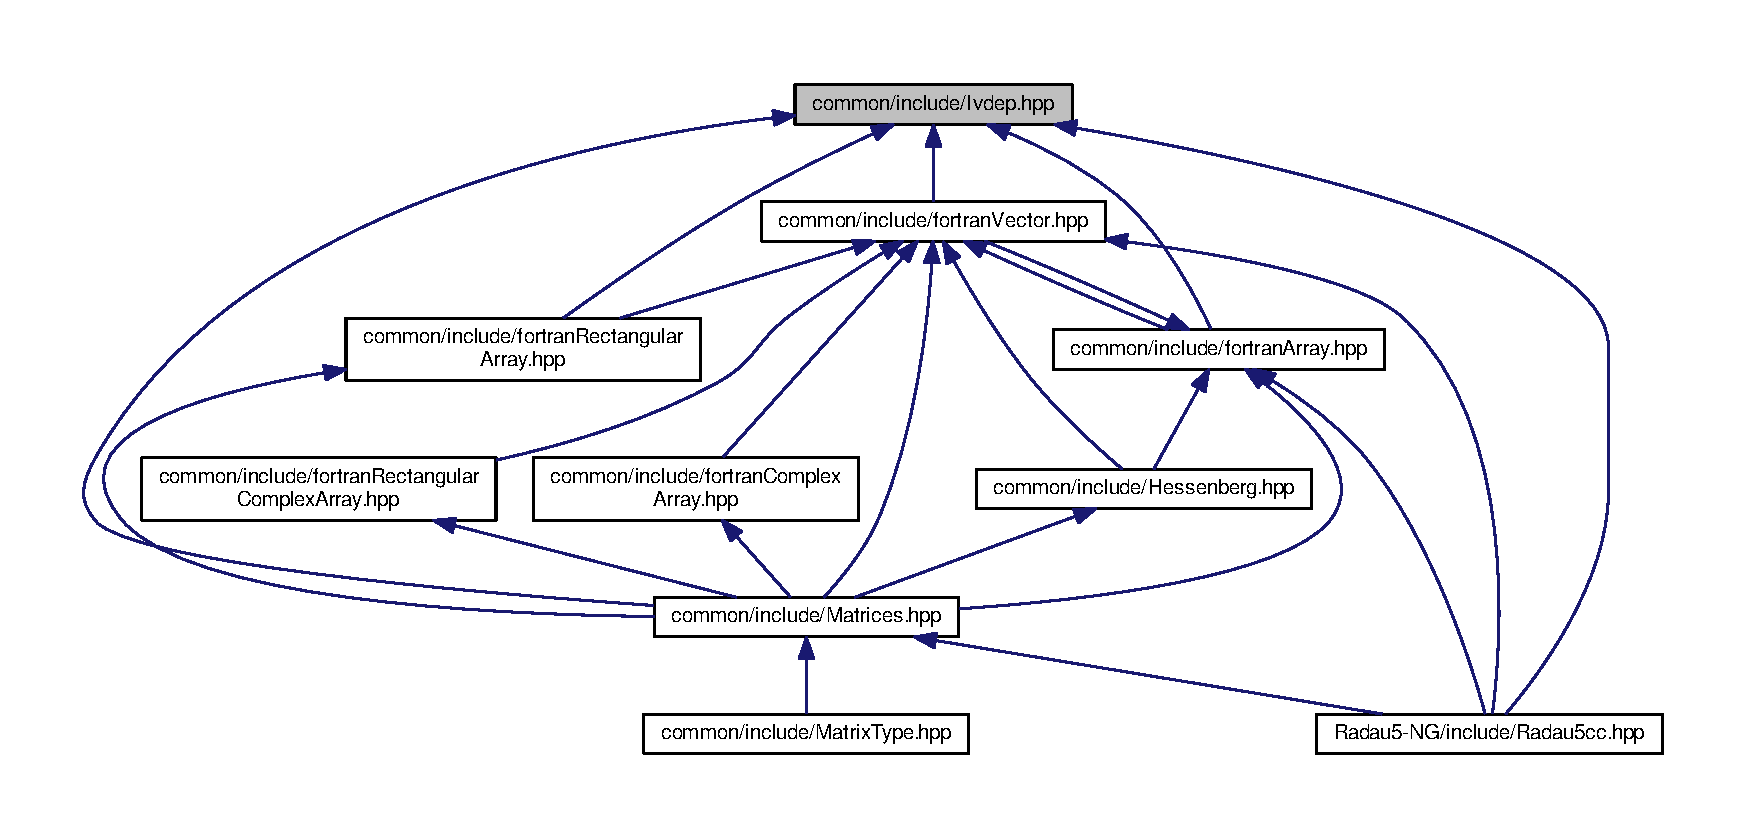
\includegraphics[width=350pt]{Ivdep_8hpp__dep__incl}
\end{center}
\end{figure}

\hypertarget{logger_8hpp}{\section{common/include/logger.hpp File Reference}
\label{logger_8hpp}\index{common/include/logger.\-hpp@{common/include/logger.\-hpp}}
}
{\ttfamily \#include $<$list$>$}\\*
{\ttfamily \#include $<$iostream$>$}\\*
{\ttfamily \#include $<$string$>$}\\*
Include dependency graph for logger.\-hpp\-:\nopagebreak
\begin{figure}[H]
\begin{center}
\leavevmode
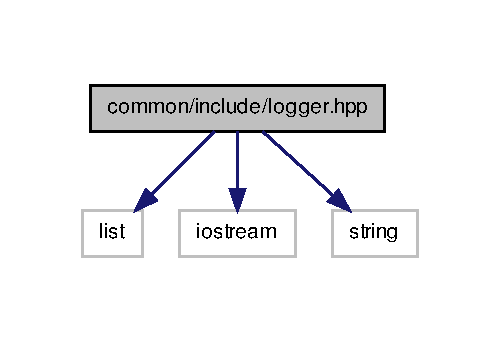
\includegraphics[width=240pt]{logger_8hpp__incl}
\end{center}
\end{figure}
\subsection*{Classes}
\begin{DoxyCompactItemize}
\item 
class \hyperlink{classodes_1_1logger}{odes\-::logger}
\begin{DoxyCompactList}\small\item\em For logging events. \end{DoxyCompactList}\item 
struct \hyperlink{structodes_1_1logger_1_1event}{odes\-::logger\-::event}
\end{DoxyCompactItemize}
\subsection*{Namespaces}
\begin{DoxyCompactItemize}
\item 
\hyperlink{namespaceodes}{odes}
\begin{DoxyCompactList}\small\item\em Compute all matrix operations. \end{DoxyCompactList}\end{DoxyCompactItemize}
\subsection*{Enumerations}
\begin{DoxyCompactItemize}
\item 
enum \hyperlink{namespaceodes_a0e9924dcd4d2b0cedc36ec2eff4dcba8}{odes\-::event\-Type} \{ \\*
\hyperlink{namespaceodes_a0e9924dcd4d2b0cedc36ec2eff4dcba8ad4b896da4797189f441c09833809cd9b}{odes\-::success} =0, 
\hyperlink{namespaceodes_a0e9924dcd4d2b0cedc36ec2eff4dcba8a63543747bb83162c25560885509e7ee2}{odes\-::rejected\-Step}, 
\hyperlink{namespaceodes_a0e9924dcd4d2b0cedc36ec2eff4dcba8ab34441382e71cf7d70c345be11743cee}{odes\-::\-Newton\-Failed}, 
\hyperlink{namespaceodes_a0e9924dcd4d2b0cedc36ec2eff4dcba8aa3c3a7a051ec8570634a29155a6b62e0}{odes\-::\-Newton\-Will\-Not\-Converge}, 
\\*
\hyperlink{namespaceodes_a0e9924dcd4d2b0cedc36ec2eff4dcba8a00d366881a9a224a0e426eb018f1db23}{odes\-::changed\-H}, 
\hyperlink{namespaceodes_a0e9924dcd4d2b0cedc36ec2eff4dcba8ad985883a2a443d3b103d6b312caefef2}{odes\-::all}
 \}
\end{DoxyCompactItemize}

\hypertarget{MacrosForCompilers_8hpp}{}\section{common/include/\+Macros\+For\+Compilers.hpp File Reference}
\label{MacrosForCompilers_8hpp}\index{common/include/\+Macros\+For\+Compilers.\+hpp@{common/include/\+Macros\+For\+Compilers.\+hpp}}
This graph shows which files directly or indirectly include this file\+:
\nopagebreak
\begin{figure}[H]
\begin{center}
\leavevmode
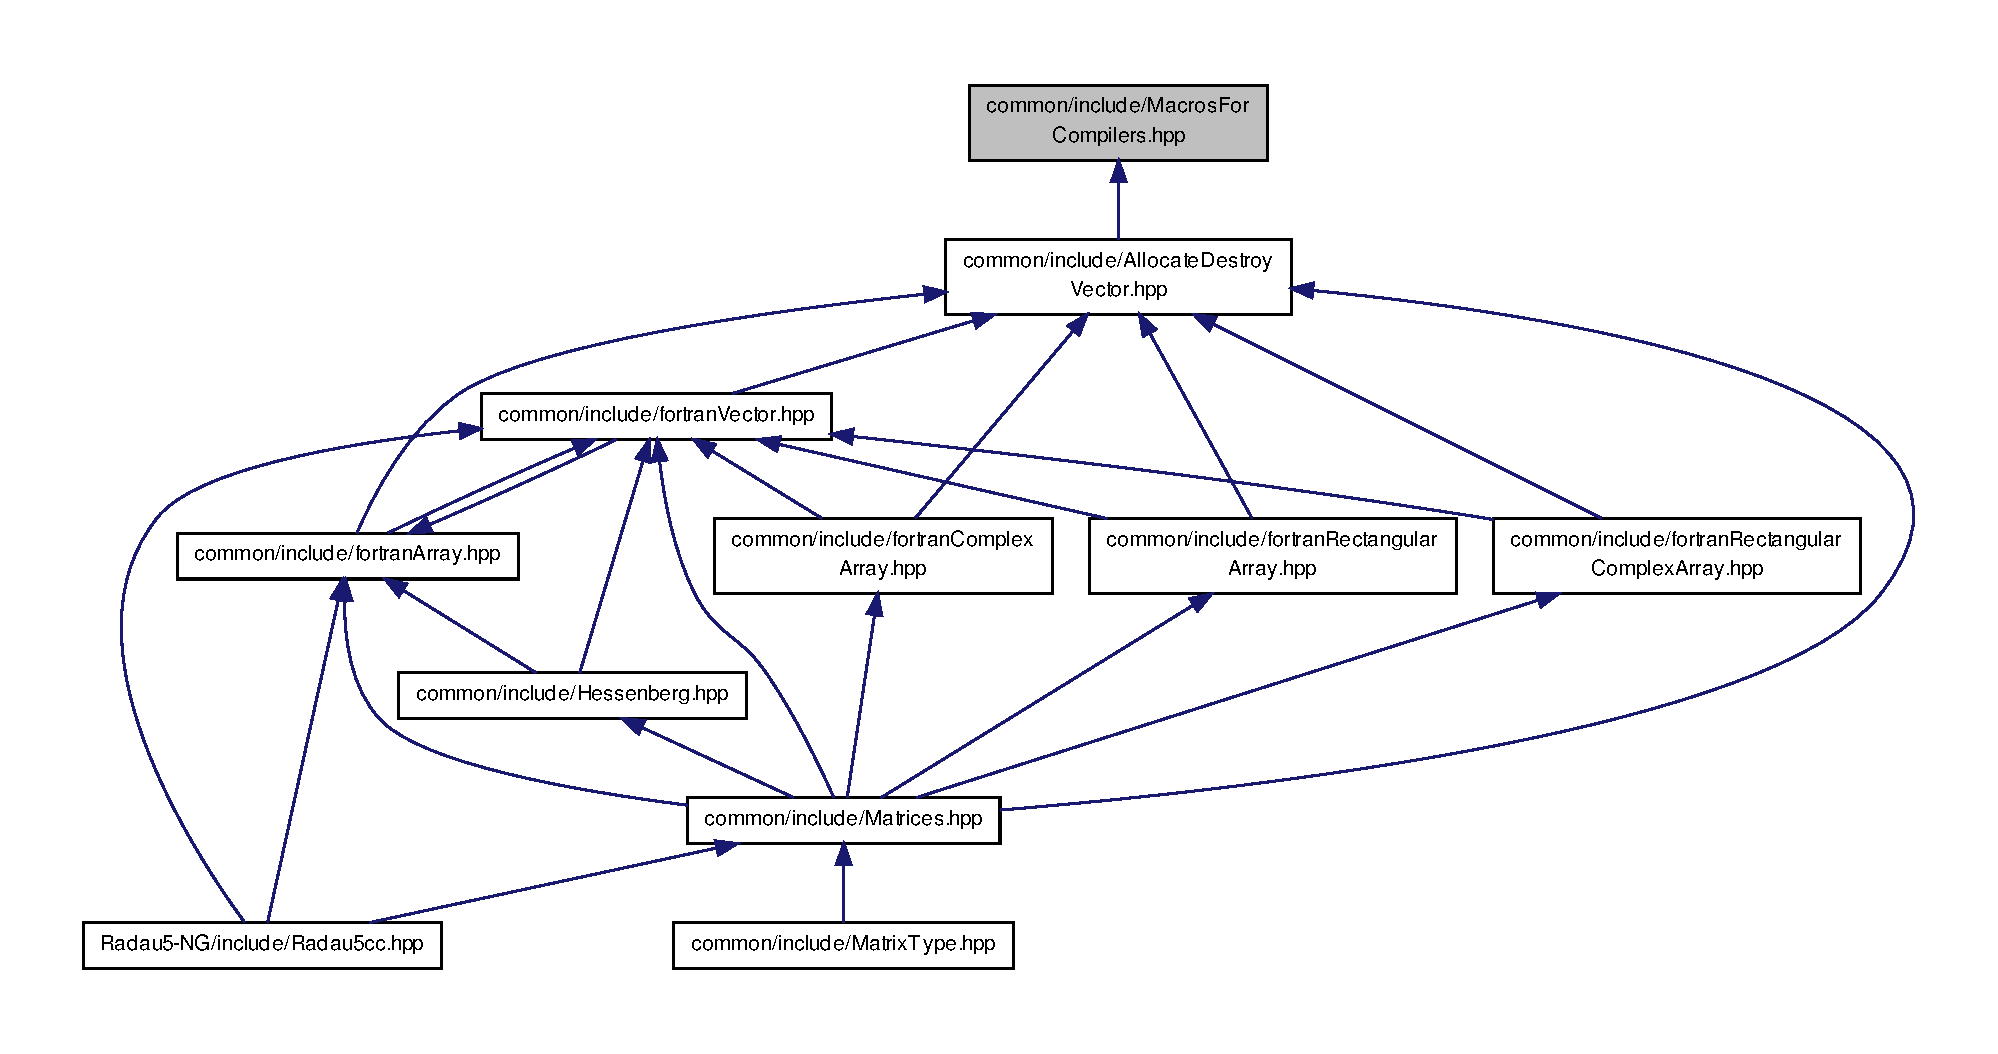
\includegraphics[width=350pt]{MacrosForCompilers_8hpp__dep__incl}
\end{center}
\end{figure}
\subsection*{Macros}
\begin{DoxyCompactItemize}
\item 
\#define \hyperlink{MacrosForCompilers_8hpp_aaa395acf51db19a6192e10ccd3c47fa2}{B\+L\+O\+C\+K\+\_\+\+F\+A\+C\+T\+O\+R}~8$\ast$sizeof(double)
\end{DoxyCompactItemize}


\subsection{Macro Definition Documentation}
\hypertarget{MacrosForCompilers_8hpp_aaa395acf51db19a6192e10ccd3c47fa2}{}\index{Macros\+For\+Compilers.\+hpp@{Macros\+For\+Compilers.\+hpp}!B\+L\+O\+C\+K\+\_\+\+F\+A\+C\+T\+O\+R@{B\+L\+O\+C\+K\+\_\+\+F\+A\+C\+T\+O\+R}}
\index{B\+L\+O\+C\+K\+\_\+\+F\+A\+C\+T\+O\+R@{B\+L\+O\+C\+K\+\_\+\+F\+A\+C\+T\+O\+R}!Macros\+For\+Compilers.\+hpp@{Macros\+For\+Compilers.\+hpp}}
\subsubsection[{B\+L\+O\+C\+K\+\_\+\+F\+A\+C\+T\+O\+R}]{\setlength{\rightskip}{0pt plus 5cm}\#define B\+L\+O\+C\+K\+\_\+\+F\+A\+C\+T\+O\+R~8$\ast$sizeof(double)}\label{MacrosForCompilers_8hpp_aaa395acf51db19a6192e10ccd3c47fa2}

\hypertarget{Matrices_8hpp}{\section{common/include/\-Matrices.hpp File Reference}
\label{Matrices_8hpp}\index{common/include/\-Matrices.\-hpp@{common/include/\-Matrices.\-hpp}}
}
{\ttfamily \#include \char`\"{}fortran\-Array.\-hpp\char`\"{}}\\*
{\ttfamily \#include \char`\"{}fortran\-Complex\-Array.\-hpp\char`\"{}}\\*
{\ttfamily \#include \char`\"{}fortran\-Rectangular\-Array.\-hpp\char`\"{}}\\*
{\ttfamily \#include \char`\"{}fortran\-Rectangular\-Complex\-Array.\-hpp\char`\"{}}\\*
{\ttfamily \#include \char`\"{}fortran\-Vector.\-hpp\char`\"{}}\\*
{\ttfamily \#include \char`\"{}Allocate\-Destroy\-Vector.\-hpp\char`\"{}}\\*
{\ttfamily \#include \char`\"{}Hessenberg.\-hpp\char`\"{}}\\*
{\ttfamily \#include \char`\"{}Generic\-Exception.\-hpp\char`\"{}}\\*
{\ttfamily \#include \char`\"{}Ivdep.\-hpp\char`\"{}}\\*
Include dependency graph for Matrices.\-hpp\-:\nopagebreak
\begin{figure}[H]
\begin{center}
\leavevmode
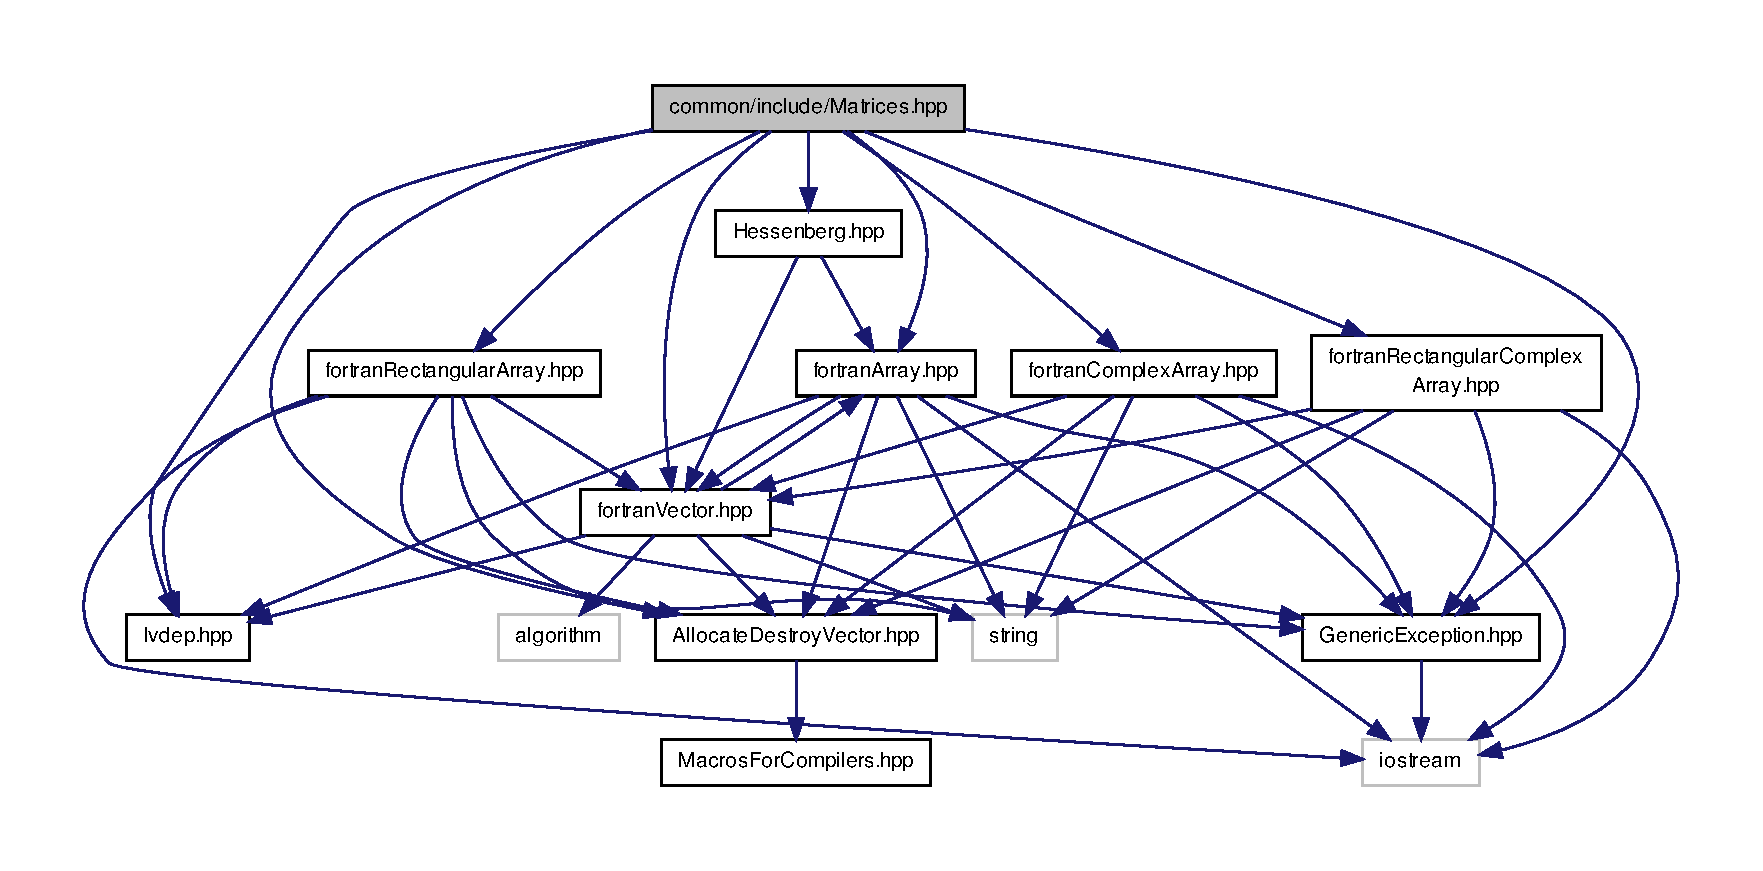
\includegraphics[width=350pt]{Matrices_8hpp__incl}
\end{center}
\end{figure}
This graph shows which files directly or indirectly include this file\-:\nopagebreak
\begin{figure}[H]
\begin{center}
\leavevmode
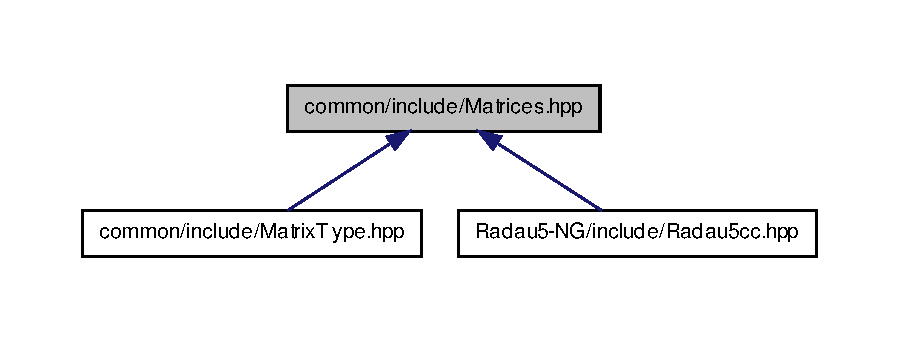
\includegraphics[width=350pt]{Matrices_8hpp__dep__incl}
\end{center}
\end{figure}
\subsection*{Classes}
\begin{DoxyCompactItemize}
\item 
class \hyperlink{classodes_1_1Matrices}{odes\-::\-Matrices$<$ full, Hessengerg, n, nsub, nsup $>$}
\begin{DoxyCompactList}\small\item\em full matrices. \end{DoxyCompactList}\item 
class \hyperlink{classodes_1_1Matrices_3_01false_00_01false_00_01n_00_01nsub_00_01nsup_01_4}{odes\-::\-Matrices$<$ false, false, n, nsub, nsup $>$}
\item 
class \hyperlink{classodes_1_1Matrices_3_01true_00_01true_00_01n_00_01nsub_00_01nsup_01_4}{odes\-::\-Matrices$<$ true, true, n, nsub, nsup $>$}
\begin{DoxyCompactList}\small\item\em Full matrices, Hessenberg=true. \end{DoxyCompactList}\item 
class \hyperlink{classodes_1_1Matrices_3_01false_00_01true_00_01n_00_01nsub_00_01nsup_01_4}{odes\-::\-Matrices$<$ false, true, n, nsub, nsup $>$}
\begin{DoxyCompactList}\small\item\em Banded matrices, Hessenberg=true\-: error. \end{DoxyCompactList}\end{DoxyCompactItemize}
\subsection*{Namespaces}
\begin{DoxyCompactItemize}
\item 
\hyperlink{namespaceodes}{odes}
\begin{DoxyCompactList}\small\item\em Compute all matrix operations. \end{DoxyCompactList}\end{DoxyCompactItemize}
\subsection*{Macros}
\begin{DoxyCompactItemize}
\item 
\#define \hyperlink{Matrices_8hpp_aacc3ee1a7f283f8ef65cea31f4436a95}{M\-A\-X}(x, y)~((x)$>$(y)?(x)\-:(y))
\item 
\#define \hyperlink{Matrices_8hpp_a74e75242132eaabbc1c512488a135926}{M\-I\-N}(x, y)~((x)$<$(y)?(x)\-:(y))
\end{DoxyCompactItemize}


\subsection{Macro Definition Documentation}
\hypertarget{Matrices_8hpp_aacc3ee1a7f283f8ef65cea31f4436a95}{\index{Matrices.\-hpp@{Matrices.\-hpp}!M\-A\-X@{M\-A\-X}}
\index{M\-A\-X@{M\-A\-X}!Matrices.hpp@{Matrices.\-hpp}}
\subsubsection[{M\-A\-X}]{\setlength{\rightskip}{0pt plus 5cm}\#define M\-A\-X(
\begin{DoxyParamCaption}
\item[{}]{x, }
\item[{}]{y}
\end{DoxyParamCaption}
)~((x)$>$(y)?(x)\-:(y))}}\label{Matrices_8hpp_aacc3ee1a7f283f8ef65cea31f4436a95}
\hypertarget{Matrices_8hpp_a74e75242132eaabbc1c512488a135926}{\index{Matrices.\-hpp@{Matrices.\-hpp}!M\-I\-N@{M\-I\-N}}
\index{M\-I\-N@{M\-I\-N}!Matrices.hpp@{Matrices.\-hpp}}
\subsubsection[{M\-I\-N}]{\setlength{\rightskip}{0pt plus 5cm}\#define M\-I\-N(
\begin{DoxyParamCaption}
\item[{}]{x, }
\item[{}]{y}
\end{DoxyParamCaption}
)~((x)$<$(y)?(x)\-:(y))}}\label{Matrices_8hpp_a74e75242132eaabbc1c512488a135926}

\hypertarget{MatrixType_8hpp}{}\section{common/include/\+Matrix\+Type.hpp File Reference}
\label{MatrixType_8hpp}\index{common/include/\+Matrix\+Type.\+hpp@{common/include/\+Matrix\+Type.\+hpp}}
{\ttfamily \#include \char`\"{}Matrices.\+hpp\char`\"{}}\\*
Include dependency graph for Matrix\+Type.\+hpp\+:
\nopagebreak
\begin{figure}[H]
\begin{center}
\leavevmode
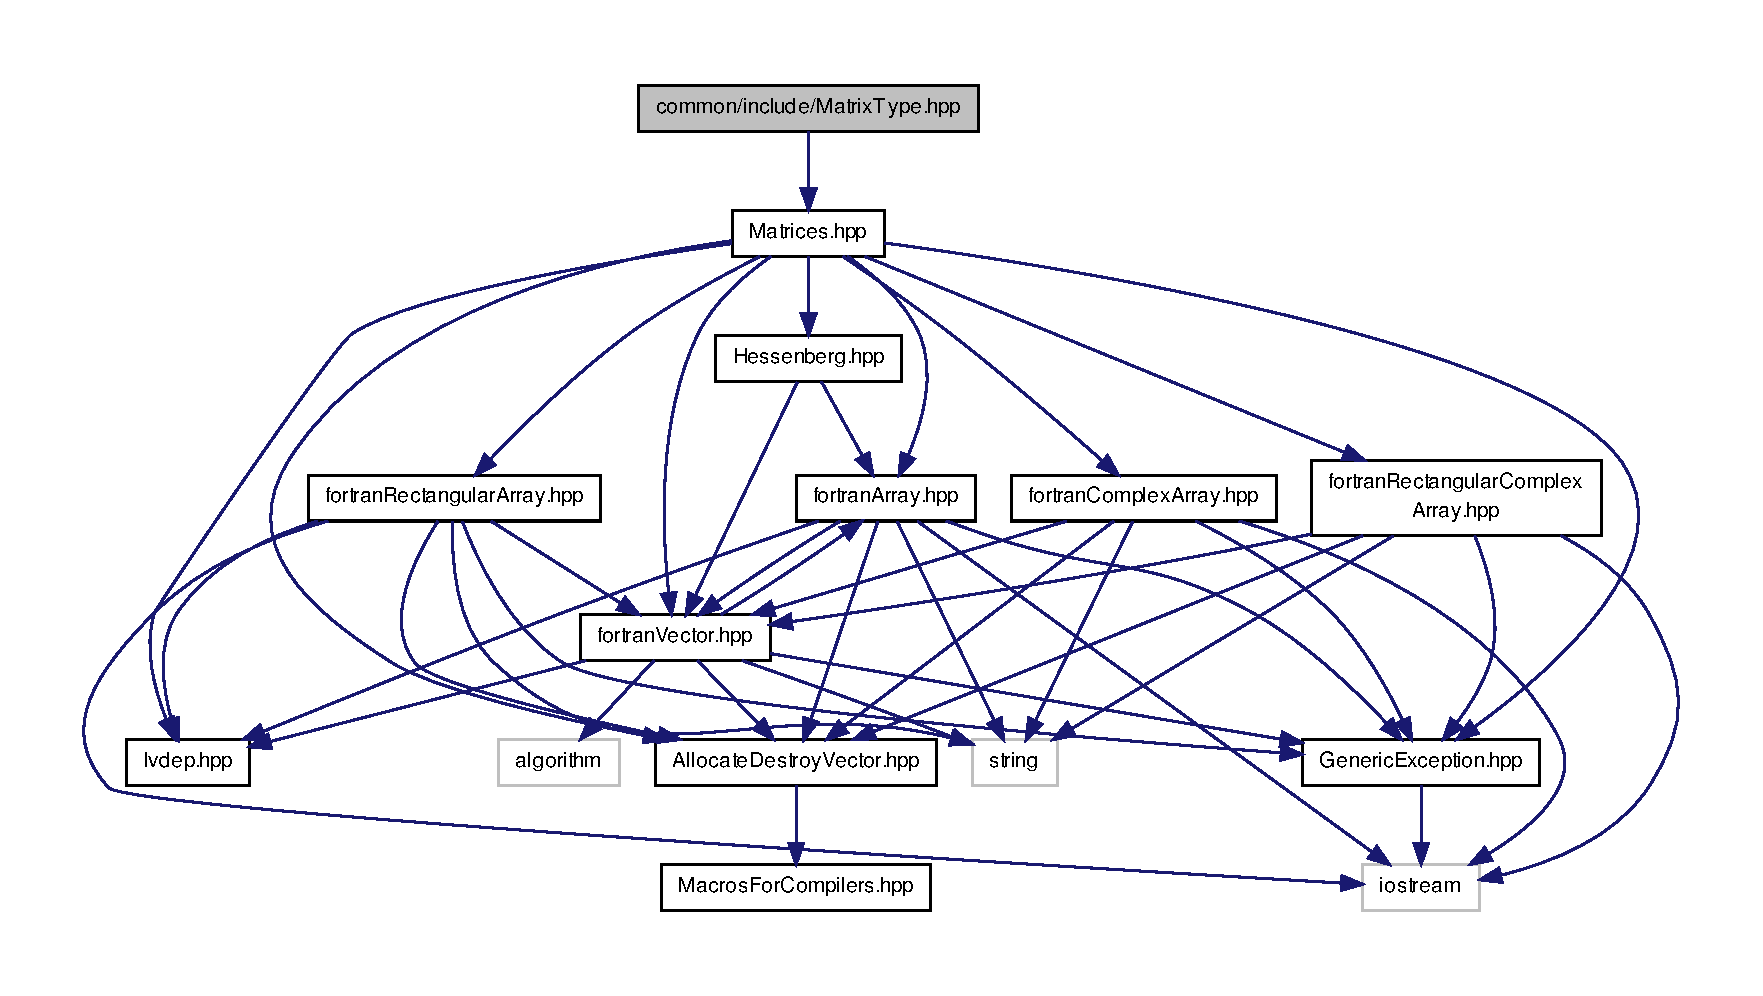
\includegraphics[width=350pt]{MatrixType_8hpp__incl}
\end{center}
\end{figure}
\subsection*{Classes}
\begin{DoxyCompactItemize}
\item 
struct \hyperlink{structodes_1_1Matrixtype}{odes\+::\+Matrixtype$<$ n, nsub, nsup $>$}
\end{DoxyCompactItemize}
\subsection*{Namespaces}
\begin{DoxyCompactItemize}
\item 
 \hyperlink{namespaceodes}{odes}
\begin{DoxyCompactList}\small\item\em Compute all matrix operations. \end{DoxyCompactList}\end{DoxyCompactItemize}

\hypertarget{protos__lapack_8hpp}{}\section{common/include/protos\+\_\+lapack.hpp File Reference}
\label{protos__lapack_8hpp}\index{common/include/protos\+\_\+lapack.\+hpp@{common/include/protos\+\_\+lapack.\+hpp}}
This graph shows which files directly or indirectly include this file\+:
\nopagebreak
\begin{figure}[H]
\begin{center}
\leavevmode
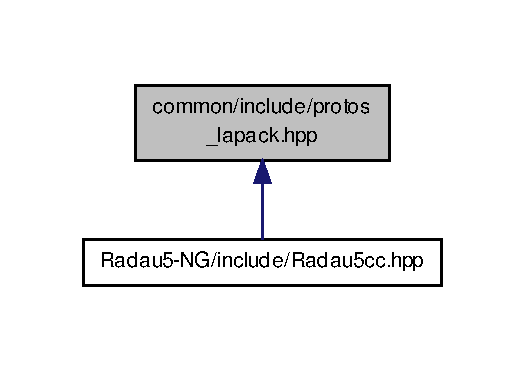
\includegraphics[width=246pt]{protos__lapack_8hpp__dep__incl}
\end{center}
\end{figure}
\subsection*{Namespaces}
\begin{DoxyCompactItemize}
\item 
 \hyperlink{namespaceodes}{odes}
\begin{DoxyCompactList}\small\item\em Compute all matrix operations. \end{DoxyCompactList}\end{DoxyCompactItemize}
\subsection*{Functions}
\begin{DoxyCompactItemize}
\item 
void \hyperlink{namespaceodes_af0b7a0203a69c4fa322079ad196cdcae}{odes\+::dgetrf\+\_\+} (int $\ast$n, int $\ast$m, double $\ast$a, int $\ast$lda, int $\ast$ipiv, int $\ast$info)
\begin{DoxyCompactList}\small\item\em prototypes for lapack routines. \end{DoxyCompactList}\item 
void \hyperlink{namespaceodes_a68cd3ad2ee6d143463ea0a41971b45ca}{odes\+::zgetrf\+\_\+} (int $\ast$n, int $\ast$m, double $\ast$a, int $\ast$lda, int $\ast$ipiv, int $\ast$info)
\item 
void \hyperlink{namespaceodes_acb38308231063d618ca8f4bfcf8f3912}{odes\+::dgetrs\+\_\+} (const char $\ast$s, int $\ast$N, int $\ast$N\+R\+H\+S, double $\ast$A, int $\ast$L\+D\+A, int $\ast$I\+P\+I\+V, double $\ast$B, int $\ast$L\+D\+B, int $\ast$I\+N\+F\+O)
\item 
void \hyperlink{namespaceodes_ab6f6bedf50ce1e3b9e01f7cacbd5a9a8}{odes\+::zgetrs\+\_\+} (const char $\ast$s, int $\ast$N, int $\ast$N\+R\+H\+S, double $\ast$A, int $\ast$L\+D\+A, int $\ast$I\+P\+I\+V, double $\ast$B, int $\ast$L\+D\+B, int $\ast$I\+N\+F\+O)
\item 
void \hyperlink{namespaceodes_a84c781070989698cdb58c37a5074a91c}{odes\+::dgbtrf\+\_\+} (int $\ast$n, int $\ast$m, int $\ast$k1, int $\ast$k2, double $\ast$a, int $\ast$lda, int $\ast$ipiv, int $\ast$info)
\item 
void \hyperlink{namespaceodes_ae9a95c96e0823f5ac279e572fba93550}{odes\+::zgbtrf\+\_\+} (int $\ast$n, int $\ast$m, int $\ast$k1, int $\ast$k2, double $\ast$a, int $\ast$lda, int $\ast$ipiv, int $\ast$info)
\item 
void \hyperlink{namespaceodes_a8ef9d46ddb5b78777217d2162ac4470f}{odes\+::dgbtrs\+\_\+} (const char $\ast$s, int $\ast$N, int $\ast$k1, int $\ast$k2, int $\ast$N\+R\+H\+S, double $\ast$A, int $\ast$L\+D\+A, int $\ast$I\+P\+I\+V, double $\ast$B, int $\ast$L\+D\+B, int $\ast$I\+N\+F\+O)
\item 
void \hyperlink{namespaceodes_ad56f5a1a4c30315e999fb0c3f1be7c24}{odes\+::zgbtrs\+\_\+} (const char $\ast$s, int $\ast$N, int $\ast$k1, int $\ast$k2, int $\ast$N\+R\+H\+S, double $\ast$A, int $\ast$L\+D\+A, int $\ast$I\+P\+I\+V, double $\ast$B, int $\ast$L\+D\+B, int $\ast$I\+N\+F\+O)
\item 
void \hyperlink{namespaceodes_aee13c6130981afb5d561ed5a7d61f523}{odes\+::dlarnv\+\_\+} (int $\ast$idist, int iseed\mbox{[}$\,$\mbox{]}, int $\ast$n, double $\ast$x)
\item 
void \hyperlink{namespaceodes_a8e1a54591e1e244caf5bdda4a798210d}{odes\+::dgehrd\+\_\+} (int $\ast$n, int $\ast$ilo, int $\ast$ihi, double $\ast$a, int $\ast$lda, double tau\mbox{[}$\,$\mbox{]}, double work\mbox{[}$\,$\mbox{]}, int $\ast$lwork, int $\ast$info)
\item 
void \hyperlink{namespaceodes_adff449269843fe4af255e0956be12fd0}{odes\+::dorghr\+\_\+} (int $\ast$n, int $\ast$ilo, int $\ast$ihi, double $\ast$a, int $\ast$lda, double tau\mbox{[}$\,$\mbox{]}, double work\mbox{[}$\,$\mbox{]}, int $\ast$lwork, int $\ast$info)
\item 
void \hyperlink{namespaceodes_aff86990f12f528839d2ff3b40ed98b1a}{odes\+::dgeev\+\_\+} (const char $\ast$jobvl, const char $\ast$jobvr, int $\ast$n, double $\ast$a, int $\ast$lda, double $\ast$W\+R, double $\ast$W\+I, double $\ast$V\+L, int $\ast$L\+D\+V\+L, double $\ast$V\+R, int $\ast$L\+D\+V\+R, double $\ast$W\+O\+R\+K, int $\ast$L\+W\+O\+R\+K, int $\ast$I\+N\+F\+O)
\end{DoxyCompactItemize}

\hypertarget{mainpage_8dox}{}\section{Mainpage/mainpage.dox File Reference}
\label{mainpage_8dox}\index{Mainpage/mainpage.\+dox@{Mainpage/mainpage.\+dox}}

\hypertarget{Radau5cc_8hpp}{}\section{Radau5-\/\+N\+G/include/\+Radau5cc.hpp File Reference}
\label{Radau5cc_8hpp}\index{Radau5-\/\+N\+G/include/\+Radau5cc.\+hpp@{Radau5-\/\+N\+G/include/\+Radau5cc.\+hpp}}
{\ttfamily \#include \char`\"{}Generic\+Exception.\+hpp\char`\"{}}\\*
{\ttfamily \#include \char`\"{}fortran\+Array.\+hpp\char`\"{}}\\*
{\ttfamily \#include \char`\"{}fortran\+Vector.\+hpp\char`\"{}}\\*
{\ttfamily \#include \char`\"{}protos\+\_\+lapack.\+hpp\char`\"{}}\\*
{\ttfamily \#include \char`\"{}Matrices.\+hpp\char`\"{}}\\*
{\ttfamily \#include \char`\"{}compat.\+hpp\char`\"{}}\\*
{\ttfamily \#include $<$cmath$>$}\\*
{\ttfamily \#include $<$utility$>$}\\*
{\ttfamily \#include \char`\"{}Ivdep.\+hpp\char`\"{}}\\*
Include dependency graph for Radau5cc.\+hpp\+:
\nopagebreak
\begin{figure}[H]
\begin{center}
\leavevmode
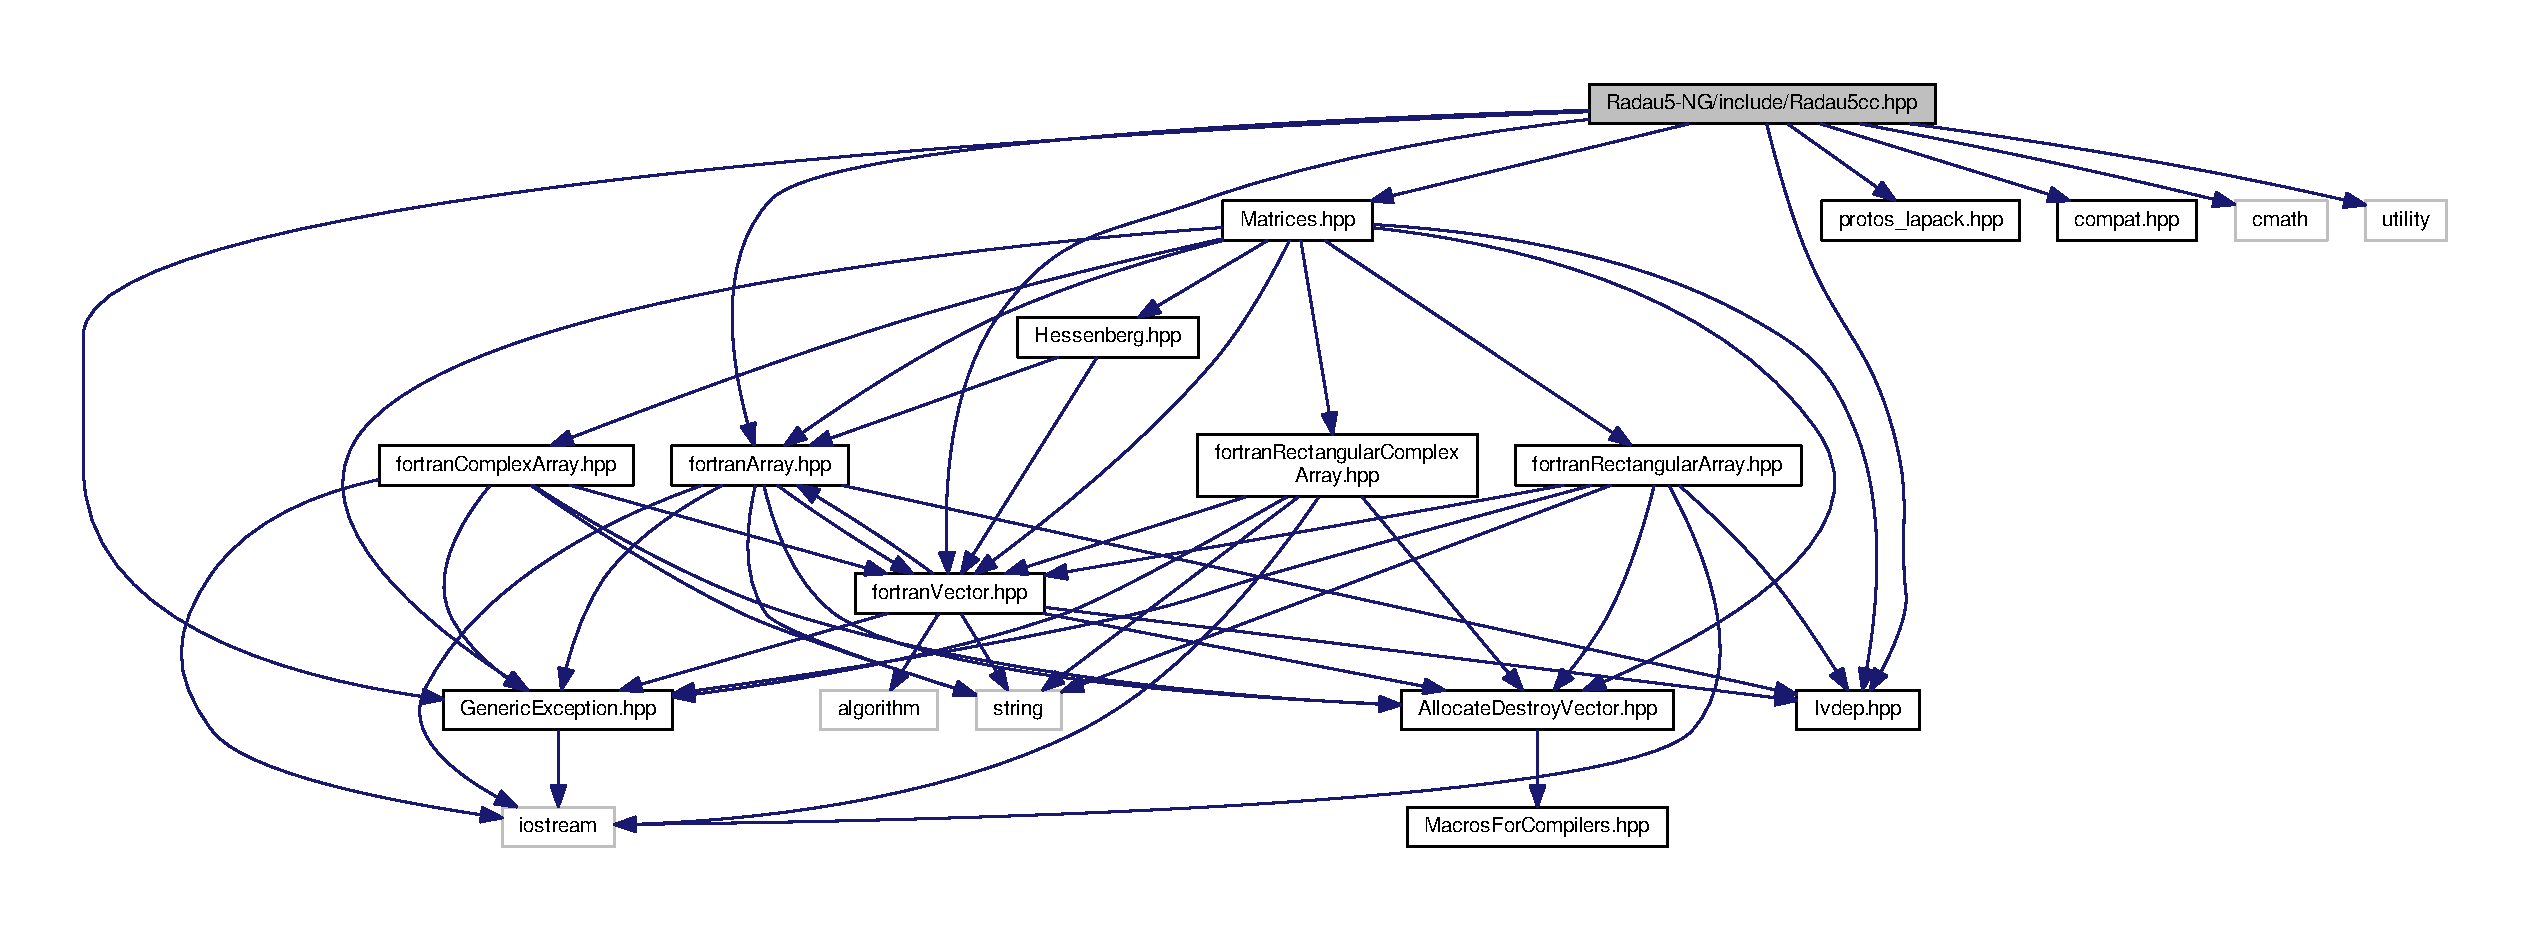
\includegraphics[width=350pt]{Radau5cc_8hpp__incl}
\end{center}
\end{figure}
\subsection*{Classes}
\begin{DoxyCompactItemize}
\item 
class \hyperlink{classodes_1_1Radau5cc}{odes\+::\+Radau5cc$<$ Fonct $>$}
\begin{DoxyCompactList}\small\item\em A C++ implementation of Radau5. \end{DoxyCompactList}\end{DoxyCompactItemize}
\subsection*{Namespaces}
\begin{DoxyCompactItemize}
\item 
 \hyperlink{namespaceodes}{odes}
\begin{DoxyCompactList}\small\item\em Compute all matrix operations. \end{DoxyCompactList}\end{DoxyCompactItemize}
\subsection*{Macros}
\begin{DoxyCompactItemize}
\item 
\#define \hyperlink{Radau5cc_8hpp_aacc3ee1a7f283f8ef65cea31f4436a95}{M\+A\+X}(x,  y)~((x)$>$(y)?(x)\+:(y))
\item 
\#define \hyperlink{Radau5cc_8hpp_a74e75242132eaabbc1c512488a135926}{M\+I\+N}(x,  y)~((x)$<$(y)?(x)\+:(y))
\item 
\#define \hyperlink{Radau5cc_8hpp_ae2f08dc603ae93c402abd918ba4e23e1}{A\+B\+S}(a)~(((a) $>$= (0.\+0)) ? (a) \+: (-\/a))
\item 
\#define \hyperlink{Radau5cc_8hpp_a8c4a9e5e4622948245de4ec0b5d38329}{S\+I\+G\+N}(a)~(((a) $>$= (0.\+0)) ? (1.) \+: (-\/1.))
\end{DoxyCompactItemize}


\subsection{Macro Definition Documentation}
\hypertarget{Radau5cc_8hpp_ae2f08dc603ae93c402abd918ba4e23e1}{}\index{Radau5cc.\+hpp@{Radau5cc.\+hpp}!A\+B\+S@{A\+B\+S}}
\index{A\+B\+S@{A\+B\+S}!Radau5cc.\+hpp@{Radau5cc.\+hpp}}
\subsubsection[{A\+B\+S}]{\setlength{\rightskip}{0pt plus 5cm}\#define A\+B\+S(
\begin{DoxyParamCaption}
\item[{}]{a}
\end{DoxyParamCaption}
)~(((a) $>$= (0.\+0)) ? (a) \+: (-\/a))}\label{Radau5cc_8hpp_ae2f08dc603ae93c402abd918ba4e23e1}
\hypertarget{Radau5cc_8hpp_aacc3ee1a7f283f8ef65cea31f4436a95}{}\index{Radau5cc.\+hpp@{Radau5cc.\+hpp}!M\+A\+X@{M\+A\+X}}
\index{M\+A\+X@{M\+A\+X}!Radau5cc.\+hpp@{Radau5cc.\+hpp}}
\subsubsection[{M\+A\+X}]{\setlength{\rightskip}{0pt plus 5cm}\#define M\+A\+X(
\begin{DoxyParamCaption}
\item[{}]{x, }
\item[{}]{y}
\end{DoxyParamCaption}
)~((x)$>$(y)?(x)\+:(y))}\label{Radau5cc_8hpp_aacc3ee1a7f283f8ef65cea31f4436a95}
\hypertarget{Radau5cc_8hpp_a74e75242132eaabbc1c512488a135926}{}\index{Radau5cc.\+hpp@{Radau5cc.\+hpp}!M\+I\+N@{M\+I\+N}}
\index{M\+I\+N@{M\+I\+N}!Radau5cc.\+hpp@{Radau5cc.\+hpp}}
\subsubsection[{M\+I\+N}]{\setlength{\rightskip}{0pt plus 5cm}\#define M\+I\+N(
\begin{DoxyParamCaption}
\item[{}]{x, }
\item[{}]{y}
\end{DoxyParamCaption}
)~((x)$<$(y)?(x)\+:(y))}\label{Radau5cc_8hpp_a74e75242132eaabbc1c512488a135926}
\hypertarget{Radau5cc_8hpp_a8c4a9e5e4622948245de4ec0b5d38329}{}\index{Radau5cc.\+hpp@{Radau5cc.\+hpp}!S\+I\+G\+N@{S\+I\+G\+N}}
\index{S\+I\+G\+N@{S\+I\+G\+N}!Radau5cc.\+hpp@{Radau5cc.\+hpp}}
\subsubsection[{S\+I\+G\+N}]{\setlength{\rightskip}{0pt plus 5cm}\#define S\+I\+G\+N(
\begin{DoxyParamCaption}
\item[{}]{a}
\end{DoxyParamCaption}
)~(((a) $>$= (0.\+0)) ? (1.) \+: (-\/1.))}\label{Radau5cc_8hpp_a8c4a9e5e4622948245de4ec0b5d38329}

%--- End generated contents ---

% Index
\newpage
\phantomsection
\addcontentsline{toc}{chapter}{Index}
\printindex

\end{document}
